\documentclass[english,xcolor={rgb,dvipsnames,table,usenames}, presentation]{beamer}

\setbeamertemplate{navigation symbols}{}

\mode<beamer> {

\usecolortheme{magpie}
\setbeamercolor{normal text}{fg=white}
\usebeamercolor[fg]{normal text}
\usepackage{pgfpages}
\setbeameroption{show notes}
\setbeameroption{show notes on second screen=right}
\setbeamerfont{note page}{size=\footnotesize}


}


\mode<handout> {

\usecolortheme{beaver}
\setbeamercolor{normal text}{fg=black}
\usebeamercolor[fg]{normal text}
\renewcommand{\textcolor}[1]{}
\usepackage{pgfpages}
\setbeameroption{show notes}
\setbeameroption{show notes on second screen=right}
\setbeamerfont{note page}{size=\footnotesize}
\setbeameroption{show only notes}

}



\usepackage{colortbl}
\usepackage{cancel}
\usepackage{multirow}
\usepackage{graphicx}
\usepackage{booktabs}
\usepackage[utf8]{inputenc}
\usepackage[T1]{fontenc}
\usepackage{colortbl}
\usepackage{pgfplots}
\usepackage{array,multirow,makecell}
\usepackage{dsfont}
\usepackage{stmaryrd}
\usepackage{multicol}
\usepackage{changepage}
\usepackage{amsmath}
\usepackage{amssymb}
\usepackage{amsfonts}
\usepackage{bm}
\usepackage[export]{adjustbox}
\usepackage{slashbox}
\usepackage{xcolor}
\usepackage{pict2e}
\usepackage{pifont}
\usepackage{eurosym}
\usepackage{tikz}
\usepackage{ulem}
\usepackage[customcolors]{hf-tikz}
\usetikzlibrary{arrows,intersections,positioning,shapes.arrows,decorations.markings}
\usepackage{hyperref}
\usepackage{mdframed}
\usepackage{listings}
\usepackage{caption}
\usepackage{subcaption}
\usepackage[backend=biber,bibencoding=utf8,citestyle=authortitle-ibid]{biblatex}
\usepackage{animate}
\usepackage{listings}
\usepackage{appendixnumberbeamer}
\usetikzlibrary{calc}
\usetikzlibrary{hobby}
\makeatletter % from https://tex.stackexchange.com/a/283273/121799
% Here we define the comparison macro for pairs (a,b)
% We assume decimal numbers acceptable to \ifdim tests
\long\def\xintdothis #1#2\xintorthat #3{\fi #1}%
\let\xintorthat \@firstofone

\captionsetup[figure]{labelfont={color=orange}}

\long\def\@thirdoffour  #1#2#3#4{#3}%
\long\def\@fourthoffour #1#2#3#4{#4}%

\def\IfFirstPairIsGreaterTF #1#2{\@IfFirstPairIsGreaterTF #1,#2,}%

\def\@IfFirstPairIsGreaterTF #1,#2,#3,#4,{%
    \ifdim #1\p@=#3\p@
       \xintdothis{%
         \ifdim #2\p@>#4\p@\expandafter\@firstoftwo
         \else\expandafter\@secondoftwo\fi}\fi
    \ifdim #1\p@>#3\p@\expandafter\@thirdoffour
                      \else\expandafter\@fourthoffour\fi
    \xintorthat{}%
}%

% not needed for numerical inputs
% \catcode`! 3
% \catcode`? 3

% Here there is a very strange \romannumeral0\romannumeral0, this is
% due to some convoluted scheme to avoid double spaces or no spaces
% in between coordinate pairs. Trust me.
\def\QSpairs {\romannumeral0\romannumeral0\qspairs }%
% first we check if empty list
\def\qspairs   #1{\expandafter\qspairs@a\romannumeral-`0#1(!)(?)}%
\def\qspairs@a #1(#2{\ifx!#2\expandafter\qspairs@abort\else
                        \expandafter\qspairs@b\fi (#2}%
\edef\qspairs@abort #1(?){\space\space}%
%
% we check if empty of single and if not pick up the first as Pivot:
\def\qspairs@b #1(#2)#3(#4){\ifx?#4\xintdothis\qspairs@empty\fi
                   \ifx!#4\xintdothis\qspairs@single\fi
                   \xintorthat \qspairs@separate {}{}{#2}(#4)}%
\def\qspairs@empty  #1(?){ }%
\edef\qspairs@single #1#2#3#4(?){\space\space(#3)}%
\def\qspairs@separate #1#2#3#4(#5)%
{%
    \ifx!#5\expandafter\qspairs@separate@done\fi
    \IfFirstPairIsGreaterTF {#5}{#3}%
          \qspairs@separate@appendtogreater
          \qspairs@separate@appendtosmaller {#5}{#1}{#2}{#3}%
}%
%
\def\qspairs@separate@appendtogreater #1#2{\qspairs@separate {#2 (#1)}}%
\def\qspairs@separate@appendtosmaller #1#2#3{\qspairs@separate {#2}{#3 (#1)}}%
%
\def\qspairs@separate@done\IfFirstPairIsGreaterTF #1#2%
    \qspairs@separate@appendtogreater
    \qspairs@separate@appendtosmaller #3#4#5#6(?)%
{%
    \expandafter\qspairs@f\expandafter
    {\romannumeral0\qspairs@b #4(!)(?)}{\qspairs@b #5(!)(?)}{ (#2)}%
}%
%
\def\qspairs@f #1#2#3{#2#3#1}%
%
% \catcode`! 12
% \catcode`? 12

\makeatother
\makeatletter % from https://tex.stackexchange.com/a/412901/121799
\newcommand{\Distance}[3]{% % from https://tex.stackexchange.com/q/56353/121799
\tikz@scan@one@point\pgfutil@firstofone($#1-#2$)\relax  
\pgfmathsetmacro{#3}{veclen(\the\pgf@x,\the\pgf@y)/28.45274}
}
\makeatother 
\newcount\nbofwords
\makeatletter% from https://tex.stackexchange.com/a/12819/121799
\def\myutil@empty{}
\def\multiwords#1 #2\@nil{% 
 \def\NextArg{#2}%
 \advance\nbofwords by  1 %   
 \expandafter\edef\csname word\@alph\nbofwords\endcsname{#1}% 
 \ifx\myutil@empty\NextArg
     \let\next\@gobble
 \fi
 \next#2\@nil
}%    
\def\GetWords#1{%
   \let\next\multiwords 
   \nbofwords=0 %
   \expandafter\next#1 \@nil %
}% 
\makeatother

\long\def\First(#1,#2){#1}
\long\def\Second(#1,#2){#2}
\tikzset{declare
function={interpolator(\x,\xmin,\xmax,\rmin,\rmax)=(\rmin+\rmax)/2+((\rmin-\rmax)/2)*cos((\x-\xmin)*(180/(\xmax-\xmin)));}}
%\tikzset{declare function={PotatoeRadius(\x,\angleA,\angleB,\angleC,\angleD,\distanceA,\distanceB,\distanceC,\distanceD)=\distanceA+(\x-\angleA)*((\distanceB-\distanceA)/(\angleB-\angleA)+(\x-\angleB)*(((-1)*((\distanceB-\distanceA)/(\angleB-\angleA))+(\distanceC-\distanceB)/(\angleC-\angleB))/(\angleC-\angleA)+(((-1)*(((-1)*((\distanceB-\distanceA)/(\angleB-\angleA))+(\distanceC-\distanceB)/(\angleC-\angleB))/(\angleC-\angleA))+((-1)*((\distanceC-\distanceB)/(\angleC-\angleB))+(\distanceD-\distanceC)/(\angleD-\angleC))/(\angleD-\angleB))*(\x-\angleC))/(\angleD-\angleA)));}}
%(\angleC*(\angleC-\angleD)*\angleD*((\distanceA-\distanceB)*(\angleC-\x)*(\angleD-\x)*\x+pow(\angleA,3)*(-(\angleC*pow(\angleD,2)*\distanceB)+\angleD*(\distanceB-\distanceC)*(\angleD-\x)*\x+\angleC*(\distanceB-\distanceD)*pow(\x,2)+pow(\angleC,2)*(\angleD*\distanceB+(-\distanceB+\distanceD)*\x))+pow(\angleB,3)*(-(\angleA*pow(\angleD,2)*\distanceC)-\angleD*(\distanceA-\distanceC)*(\angleD-\x)*\x+\angleA*(\distanceC-\distanceD)*pow(\x,2)+pow(\angleC,2)*(-(\angleD*\distanceA)+\angleA*\distanceD+\distanceA*\x-\distanceD*\x)+pow(\angleA,2)*(\angleD*\distanceC-\distanceC*\x+\distanceD*\x)+\angleC*(pow(\angleD,2)*\distanceA-pow(\angleA,2)*\distanceD+(-\distanceA+\distanceD)*pow(\x,2)))+pow(\angleA,2)*(-(\angleD*(\distanceB-\distanceC)*(\angleD-\x)*\x*(\angleD+\x))-pow(\angleC,3)*(\angleD*\distanceB+(-\distanceB+\distanceD)*\x)+\angleC*(pow(\angleD,3)*\distanceB+(-\distanceB+\distanceD)*pow(\x,3)))+\angleA*(pow(\angleD,2)*(\distanceB-\distanceC)*(\angleD-\x)*pow(\x,2)+pow(\angleC,3)*(pow(\angleD,2)*\distanceB+(-\distanceB+\distanceD)*pow(\x,2))-pow(\angleC,2)*(pow(\angleD,3)*\distanceB+(-\distanceB+\distanceD)*pow(\x,3)))+pow(\angleB,2)*(\angleD*(\distanceA-\distanceC)*(\angleD-\x)*\x*(\angleD+\x)+pow(\angleC,3)*(\angleD*\distanceA-\angleA*\distanceD-\distanceA*\x+\distanceD*\x)-pow(\angleA,3)*(\angleD*\distanceC+(-\distanceC+\distanceD)*\x)+\angleC*(-(pow(\angleD,3)*\distanceA)+pow(\angleA,3)*\distanceD+(\distanceA-\distanceD)*pow(\x,3))+\angleA*(pow(\angleD,3)*\distanceC+(-\distanceC+\distanceD)*pow(\x,3)))+\angleB*(-(pow(\angleD,2)*(\distanceA-\distanceC)*(\angleD-\x)*pow(\x,2))+pow(\angleC,3)*(-(pow(\angleD,2)*\distanceA)+pow(\angleA,2)*\distanceD+(\distanceA-\distanceD)*pow(\x,2))+pow(\angleA,3)*(pow(\angleD,2)*\distanceC+(-\distanceC+\distanceD)*pow(\x,2))+pow(\angleC,2)*(pow(\angleD,3)*\distanceA-pow(\angleA,3)*\distanceD+(-\distanceA+\distanceD)*pow(\x,3))-pow(\angleA,2)*(pow(\angleD,3)*\distanceC+(-\distanceC+\distanceD)*pow(\x,3))))/((\angleA-\angleB)*(\angleA-\angleC)*(\angleB-\angleC)*(\angleA-\angleD)*(\angleB-\angleD)*(\angleC-\angleD)));}}
\newcommand{\DrawArcAngle}[6][]{% just for emergencies
\pgfmathanglebetweenpoints{\pgfpointanchor{#3}{center}}{\pgfpointanchor{#2}{center}}
\xdef\angleA{\pgfmathresult}
\pgfmathanglebetweenpoints{\pgfpointanchor{#3}{center}}{\pgfpointanchor{#4}{center}}
\xdef\angleB{\pgfmathresult}
\draw[#1] ($(#3)+(\angleA:#5)$) arc [start angle=\angleA,end angle=\angleB,radius=#5]
#6;
}
\newcommand{\DrawPotato}[5][]{
\coordinate (PotatoCenter) at (barycentric cs:#2=1,#3=1,#4=1,#5=1);
\pgfmathanglebetweenpoints{\pgfpointanchor{PotatoCenter}{center}}{\pgfpointanchor{#2}{center}}
\xdef\angleA{\pgfmathresult}
\pgfmathanglebetweenpoints{\pgfpointanchor{PotatoCenter}{center}}{\pgfpointanchor{#3}{center}}
\xdef\angleB{\pgfmathresult}
\pgfmathanglebetweenpoints{\pgfpointanchor{PotatoCenter}{center}}{\pgfpointanchor{#4}{center}}
\xdef\angleC{\pgfmathresult}
\pgfmathanglebetweenpoints{\pgfpointanchor{PotatoCenter}{center}}{\pgfpointanchor{#5}{center}}
\xdef\angleD{\pgfmathresult}

\Distance{(PotatoCenter)}{(#2)}{\distanceA}
\Distance{(PotatoCenter)}{(#3)}{\distanceB}
\Distance{(PotatoCenter)}{(#4)}{\distanceC}
\Distance{(PotatoCenter)}{(#5)}{\distanceD}
\xdef\coordList{(\angleA,\distanceA) (\angleB,\distanceB) (\angleC,\distanceC) (\angleD,\distanceD)}%
\typeout{\coordList}
\xdef\sortedList{\QSpairs{\coordList}}%
\GetWords{\sortedList}
\xdef\NewList{\worda,\wordb,\wordc,\wordd}%
\xdef\NewList{\expandafter\First\worda/\expandafter\Second\worda, 
\expandafter\First\wordb/\expandafter\Second\wordb,
\expandafter\First\wordc/\expandafter\Second\wordc,
\expandafter\First\wordd/\expandafter\Second\wordd}% this list is not used
\xdef\angleA{\expandafter\First\worda}%
\xdef\distanceA{\expandafter\Second\worda}%
\xdef\angleB{\expandafter\First\wordb}%
\xdef\distanceB{\expandafter\Second\wordb}%
\xdef\angleC{\expandafter\First\wordc}%
\xdef\distanceC{\expandafter\Second\wordc}%
\xdef\angleD{\expandafter\First\wordd}%
\xdef\distanceD{\expandafter\Second\wordd}%
\begin{scope}[shift=(PotatoCenter)]
\draw[#1,smooth,samples=50] plot[variable=\x,domain=\angleA:\angleB] %
(\x:{interpolator(\x,\angleA,\angleB,\distanceA,\distanceB)})
-- 
plot[variable=\x,domain=\angleB:\angleC] %
(\x:{interpolator(\x,\angleB,\angleC,\distanceB,\distanceC)})
--
plot[variable=\x,domain=\angleC:\angleD] %
(\x:{interpolator(\x,\angleC,\angleD,\distanceC,\distanceD)})
--
plot[variable=\x,domain=\angleD:{\angleA+360}] %
(\x:{interpolator(\x,\angleD,{\angleA+360},\distanceD,\distanceA)});
\end{scope}
}

\definecolor{links}{HTML}{2A1B81}
\hypersetup{colorlinks,linkcolor=,urlcolor=links}

\tikzset{style green/.style={
    set fill color=green!50!lime!60,
    set border color=white,
  },
  style cyan/.style={
    set fill color=cyan!90!blue!60,
    set border color=white,
  },
  style orange/.style={
    set fill color=orange!80!red!60,
    set border color=white,
  },
  hor/.style={
    above left offset={-0.15,0.31},
    below right offset={0.15,-0.125},
    #1
  },
  ver/.style={
    above left offset={-0.1,0.3},
    below right offset={0.15,-0.15},
    #1
  }
}

\newcommand{\tikzmark}[2][minimum width=6cm,minimum height=1.5cm]{
\tikz[remember picture, overlay]
\node[anchor=west,
inner sep=0pt,
outer sep=6pt,
xshift=-0.5em,
yshift=-3ex,
#1](#2){};
}

\newcommand{\norm}[1]{\left\lVert#1\right\rVert}

\addbibresource{biblio.bib}

\newcommand{\cmark}{\ding{51}}
\newcommand{\xmark}{\ding{55}}

\setcellgapes{1pt}
\makegapedcells
\newcolumntype{R}[1]{>{\raggedleft\arraybackslash }b{#1}}
\newcolumntype{L}[1]{>{\raggedright\arraybackslash }b{#1}}
\newcolumntype{C}[1]{>{\centering\arraybackslash }b{#1}}

\DeclareMathOperator*{\argmin}{\arg\!\min}
\DeclareMathOperator*{\argmax}{\arg\!\max}

\newcommand{\xuparrow}[1]{%
  {\left\uparrow\vbox to #1{}\right.\kern-\nulldelimiterspace}
}

\renewcommand*{\bibfont}{\small}

\tikzset{
  treenode/.style = {shape=rectangle, rounded corners,
                     draw, align=center,
                     top color=white, bottom color=blue!20},
  root/.style     = {treenode, font=\Huge, bottom color=red!30},
  env/.style      = {treenode, font=\ttfamily\Large},
  dummy/.style    = {circle,draw,color=black}
}

\newcommand\rstyle{%
  \NoAutoSpacing
  \lstset{%
    language=R,
    alsoletter={_},
otherkeywords={install_github},             % Add keywords here
%    basicstyle=\small,
    keywordstyle=\color{blue},
    stringstyle=\color{green},
%    numbers=left,
%    numberstyle=\tiny,
%    numbersep=5pt,
  numbers=left,                   % where to put the line-numbers
  numberstyle=\tiny\color{blue},  % the style that is used for the line-numbers
  stepnumber=1,                   % the step between two line-numbers. If it is 1, each line
                                  % will be numbered
  numbersep=5pt,                  % how far the line-numbers are from the code
  showspaces=false,               % show spaces adding particular underscores
  showstringspaces=false,         % underline spaces within strings
  showtabs=false,                 % show tabs within strings adding particular underscores
  breaklines=true,                % sets automatic line breaking
  breakatwhitespace=false,        % sets if automatic breaks should only happen at whitespace
    frame=single%
  }%
}

\lstnewenvironment{rlisting}
{\rstyle}{}

\newcommand\rinline[1]{{\rstyle\lstinline!#1!}}

% Allows the use of \toprule, \midrule and \bottomrule in tables

%----------------------------------------------------------------------------------------
%	TITLE PAGE
%----------------------------------------------------------------------------------------

\title[Soutenance]{Formalisation et étude de problématiques \\ de scoring en risque de crédit %\\ {\vspace*{0.5cm} \small Inférence de rejet, discrétisation de variables et interactions, \\ arbres de régression logistique}}
}

\author{Soutenance de thèse d'Adrien Ehrhardt \\ {\footnotesize
Encadré par Christophe Biernacki, Philippe Heinrich, Vincent Vandewalle
}}

\institute[CACF - Inria]

\date{Villeneuve d'Ascq, 30/09/2019} % Date, can be changed to a custom date

\titlegraphic{%
    
\includegraphics[width=2.5cm]{figures/inria.png}~%
    
\includegraphics[width=4cm]{figures/logo.png}%
}

\AtBeginSection[]{
  \begin{frame}
  \vfill
  \centering
  \begin{beamercolorbox}[sep=8pt,center,shadow=true,rounded=true]{title}
    \usebeamerfont{title}\insertsectionhead\par%
  \end{beamercolorbox}
  \vfill
  \end{frame}
}

\tikzset{
    myarrow/.style={
        draw,
        fill=orange,
        single arrow,
        minimum height=3.5ex,
        single arrow head extend=1ex
    }
}

\tikzstyle{interrupt}=[
    postaction={
        decorate,
        decoration={markings,
                    mark= at position 0.5 
                          with
                          {
                            \fill[black] (-0.1,-0.3) rectangle (0.1,0.3);
                            \draw (-0.1,0.3) -- (-0.1,-0.3)
                                  (0.1,0.3) -- (0.1,-0.3);
                          }
                    }
                }
]

\newlength\mylinewidth
\setlength\mylinewidth{0.4pt}

\tikzset{
    ultra thin/.style= {line width=0.25\mylinewidth},
    very thin/.style=  {line width=0.5\mylinewidth},
    thin/.style=       {line width=\mylinewidth},
    semithick/.style=  {line width=1.5\mylinewidth},
    thick/.style=      {line width=2\mylinewidth},
    very thick/.style= {line width=3\mylinewidth},
    ultra thick/.style={line width=4\mylinewidth},
    every picture/.style={semithick}
}




\addtobeamertemplate{navigation symbols}{}{%
    \usebeamerfont{footline}%
    \usebeamercolor[fg]{footline}%
    \hspace{1em}%
    \insertframenumber/\inserttotalframenumber
}

\lstset{language=R}

\newcommand{\appropto}{\mathrel{\vcenter{
  \offinterlineskip\halign{\hfil$##$\cr
    \propto\cr\noalign{\kern2pt}\sim\cr\noalign{\kern-2pt}}}}}

\newcommand\q{{\bm{q}}}
\newcommand\s{q}
\newcommand\Q{\mathcal{Q}}
\newcommand\ag{\bm{\alpha}}
\newcommand{\bth}{\boldsymbol{\theta}} 
\newcommand{\bc}{\boldsymbol{c}} 
\newcommand{\bx}{\boldsymbol{x}} 
\newcommand{\tx}{\textbf{x}}
\newcommand{\bs}{\boldsymbol{s}} 
\newcommand{\ts}{\textbf{s}}
\newcommand{\be}{\boldsymbol{e}} 
\newcommand{\te}{\textbf{e}}
\newcommand{\by}{\boldsymbol{y}} 
\newcommand{\ty}{\textbf{y}}
\newcommand{\f}{\text{f}}
\newcommand{\nf}{\text{nf}}
\newcommand{\yslant}{0.5}
\newcommand{\xslant}{-0.6}
\newcommand{\tr}{T}
\newcommand{\bqk}{\bm{\mathfrak{q}}}

\def\mybar#1#2#3{%%
\begin{tabular}{@{}l@{}} {\scriptsize #1} \\ {\scriptsize #2} \\ {\scriptsize #3} \end{tabular} & \resizebox{.05#1\textwidth}{0.7cm}{\begin{tabular}{@{}l@{}}{\color{green}\rule[0pt]{#1bp}{10pt}} \\ {\color{orange}\rule[0pt]{#2bp}{10pt}} \\ {\color{red}\rule[0pt]{#3bp}{10pt}} \end{tabular}}}

\def\myobar#1#2#3{%%
\begin{tabular}{@{}l@{}} {\scriptsize #1} \\ {\scriptsize #2} \\ {\scriptsize #3} \end{tabular} & \resizebox{.05#2\textwidth}{0.7cm}{\begin{tabular}{@{}l@{}}{\color{orange}\rule[0pt]{#1bp}{10pt}} \\ {\color{green}\rule[0pt]{#2bp}{10pt}} \\ {\color{orange}\rule[0pt]{#3bp}{10pt}}\end{tabular}}}

\pgfmathdeclarefunction{gauss}{2}{\pgfmathparse{1/(#2*sqrt(2*pi))*exp(-((x-#1)^2)/(2*#2^2))}}

\newcommand{\myGlobalTransformation}[2]
{
    \pgftransformcm{1}{0}{0.4}{0.5}{\pgfpoint{#1cm}{#2cm}}
}


\newcommand{\myGlobalTransformationbis}[2]
{
    \pgftransformcm{1}{0}{0.4}{0.3}{\pgfpoint{#1cm}{#2cm}}
}

\newcommand{\gridThreeD}[3]
{
    \begin{scope}
        \myGlobalTransformation{#1}{#2};
        \draw [#3,step=7cm] grid (7,7);
    \end{scope}
}

\tikzstyle myBG=[line width=3pt,opacity=1.0]

\newcommand{\drawLinewithBG}[2]
{
    \draw[white,myBG]  (#1) -- (#2);
    \draw[black,very thick] (#1) -- (#2);
}

\newcommand{\graphLinesHorizontal}
{
    \drawLinewithBG{1,1}{7,1};
    \drawLinewithBG{1,3}{7,3};
    \drawLinewithBG{1,5}{7,5};
    \drawLinewithBG{1,7}{7,7};
}

\newcommand{\graphLinesVertical}
{
    %swaps x and y coordinate (hence vertical lines):
    \pgftransformcm{0}{1}{1}{0}{\pgfpoint{0cm}{0cm}}
    \graphLinesHorizontal;
}

\newcommand{\graphThreeDnodes}[2]
{
    \begin{scope}
        \myGlobalTransformation{#1}{#2};
        \foreach \x in {1,3,5,7} {
            \foreach \y in {1,3,5,7} {
                \node at (\x,\y) [circle,fill=black,scale=0.3] {};
                %this way circle of nodes will not be transformed
            }
        }
    \end{scope}
}

\begin{document}


\frame[plain]{\titlepage}

\note{Merci aux rapporteurs pour le temps consacré à la lecture du manuscrit, aux membres du jury pour leur disponibilité pour cette soutenance de thèse intitulée... 

\bigskip

On reviendra sur ce qu'on entend par scoring dans ce qui suit

\bigskip

Thèse encadrée par... préparée au sein de... Inria (équipe Modal) et, s'agissant d'une CIFRE, chez CACF}









\section{Context and notations}

\note{On se place dans la peau d'un chargé d'études statistiques qui a en face de lui un tel tableau.}

\subsection{industrial setting}

\begin{frame}<handout:0>
\frametitle{\secname: \subsecname}




%%%%%%%%%%%%%%%%%%%%
\note<1-9>{Collecte des caractéristiques de demandeurs de crédit à la consommation.

\medskip

On connaît pour certains la performance de remboursement, c-à-d les clients financés.

\medskip

On cherche à estimer une probabilité de défaut de ces emprunteurs pour l'appliquer aux nouveaux demandeurs et décider de leur acceptation crédit.

\medskip

On passe traditionnellement par 6 étapes...

\medskip

On sélectionne les variables prédictives du remboursement.

\medskip

On effectue une régression logistique et une transformation qui donne le score.

\medskip

On se donne enfin un seuil en-dessous duquel les clients sont refusés.}
%%%%%%%%%%%%%%%%%%%%




\only<1-6>{
\begin{table}
\centering
\begin{tiny}
\hspace*{-0.7cm}\begin{tabular}{p{1.7cm}|p{1.1cm}|p{1cm}|p{1.4cm}|p{1.5cm}||p{0.6cm}|p{1cm}}
\textcolor <4,6> {green} {\textbf<4,6>{Job}} & \only<1-3>{Home} & \only<1-3>{Time in job} & \textcolor <4,6> {green} {\textbf<4,6>{Family status}} & \textcolor <4,5> {green} {\textbf<4,5>{Wages}} & \only<8->{\textcolor{green}{\textbf{Score}}} & Repayment \\
\hline
\textcolor <4,6> {green} {\textbf<4,6>{\only<1-5>{Craftsman} \only<6->{?+Low-qualified}}} & \only<1-3>{Owner} & \only<1-3>{20} & \textcolor <4,6> {green} {\textbf<4,6>{\only<1-5>{Widower}  \only<6>{?+Alone}}} & \textcolor <4-5> {green} {\textbf<4-5>{\only<1-4>{2000} \only<5->{]1500;2000]}}} & \only<8->{\textcolor{green}{\textbf{225}}} & 1  \\
\textcolor <4,6> {green} {\textbf<4,6>{\only<1-5>{?} \only<6->{?+Low-qualified}}} & \only<1-3>{Renter} & \only<1-3>{10} & \textcolor <4,6> {green} {\textbf<4,6>{\only<1-5>{Common-law}  \only<6>{Union}}} & \textcolor <4-5> {green} {\textbf<4>{\only<1-4>{1700} \only<5->{]1500;2000]}}} & \only<8->{\textcolor{green}{\textbf{190}}} & 0 \\
\textcolor <4,6> {green} {\textbf<4,6>{\only<1-5>{Engineer} \only<6->{High-qualified}}} & \only<1-3>{Starter} & \only<1-3>{5} & \textcolor <4,6> {green} {\textbf<4,6>{\only<1-5>{Divorced} \only<6>{?+Alone}}} & \textcolor <4-5> {green} {\textbf<4>{\only<1-4>{4000} \only<5->{]2000;$\infty$[}}} & \only<8->{\textcolor{green}{\textbf{218}}} & 1  \\
\textcolor <4,6> {green} {\textbf<4,6>{\only<1-5>{Executive} \only<6->{High-qualified}}} & \only<1-3>{By work} & \only<1-3>{8} & \textcolor <4,6> {green} {\textbf<4,6>{\only<1-5>{Married} \only<6>{Union}}} & \textcolor <4-5> {green} {\textbf<4>{\only<1-4>{2700} \only<5->{]2000;$\infty$[}}} & \only<8->{\textcolor{green}{\textbf{202}}} & 0  \\
\textcolor <3> {green} {\textbf<3>{\only<1-2>{{Office employee}} \only<3->{\cancel{Office employee}}}} &  \textcolor <3> {green} {\textbf<3>{\only<1-2>{Renter} \only<3->{\cancel{Renter}}}} & \textcolor <3> {green} {\textbf<3>{\only<1-2>{12} \only<3->{\cancel{12}}}} & \textcolor <3> {green} {\textbf<3>{\only<1-2>{Married} \only<3->{\cancel{Married}}}} & \textcolor <3> {green} {\textbf<3>{\only<1-2>{1400} \only<3->{\cancel{1400}}}} & \only<8->{\textcolor{green}{\textbf{NA}}} & NA  \\
\textcolor <3> {green} {\textbf<3>{\only<1-2>{Worker} \only<3->{\cancel{Worker}}}} & \textcolor <3> {green} {\textbf<3>{\only<1-2>{By family} \only<3->{\cancel{By family}}}} & \textcolor <3> {green} {\textbf<3>{\only<1-2>{2} \only<3->{\cancel{2}}}} & \textcolor <3> {green} {\textbf<3>{\only<1-2>{?} \only<3->{\cancel{?}}}} & \textcolor <3> {green} {\textbf<3>{\only<1-2>{1200} \only<3->{\cancel{1200}}}} & \only<8->{{\textbf{NA}}} & NA  \\
\end{tabular}
\end{tiny}
\caption{\label{tab:exemple} Dataset with outliers and missing values.} 
\end{table}
}

\only<7>{
\begin{table}
\centering
\begin{tiny}
\hspace*{-0.7cm}\begin{tabular}{p{2cm}|p{1.1cm}|p{1cm}|p{2.4cm}||p{0.6cm}|p{1cm}}
\textcolor <4,6> {green} {\textbf<4,6>{Job}} & \only<2-3>{Home} & \only<2-3>{Time in job} & \textcolor <7> {green} {\textbf<7>{Family status x Wages}} & \only<8->{\textcolor{green}{\textbf{Score}}} & Repayment \\
\hline
\textcolor <4,6> {green} {\textbf<4,6>{\only<2-5>{Craftsman} \only<6->{?+Low-qualified}}} & \only<2-3>{Owner} & \only<2-3>{20} & \textcolor <7> {green} {\textbf<6>{?+Alone x ]1500;2000]}} & \only<8->{\textcolor{green}{\textbf{225}}} & 1  \\
\textcolor <4,6> {green} {\textbf<4,6>{\only<2-5>{?} \only<6->{?+Low-qualified}}} & \only<2-3>{Renter} & \only<2-3>{10} & \textcolor <7> {green} {\textbf<7>{Union x ]1500;2000]}} & \only<8->{\textcolor{green}{\textbf{190}}} & 0  \\
\textcolor <4,6> {green} {\textbf<4,6>{\only<2-5>{Engineer} \only<6->{High-qualified}}} & \only<2-3>{Starter} & \only<2-3>{5} & \textcolor <7> {green} {\textbf<7>{?+Alone x ]2000;$\infty$[}} & \only<8->{\textcolor{green}{\textbf{218}}} & 1  \\
\textcolor <4,6> {green} {\textbf<4,6>{\only<2-5>{Executive} \only<6->{High-qualified}}} & \only<2-3>{By work} & \only<2-3>{8} & \textcolor <7> {green} {\textbf<7>{Union x ]2000;$\infty$[}} & \only<8->{\textcolor{green}{\textbf{202}}} & 0  \\
\textcolor <3> {green} {\textbf<3>{\only<1-2>{{Office employee}} \only<3->{\cancel{Office employee}}}} &  \textcolor <3> {green} {\textbf<3>{\only<1-2>{Renter} \only<3->{\cancel{Renter}}}} & \textcolor <3> {green} {\textbf<3>{\only<1-2>{12} \only<3->{\cancel{12}}}} & \textcolor <3> {green} {\textbf<3>{\only<1-2>{Married} \only<3->{\cancel{Married}}}} \textcolor <3> {green} {\textbf<3>{\only<1-2>{1400} \only<3->{\cancel{1400}}}} & \only<8->{{\textbf{NA}}} & NA  \\
\textcolor <3> {green} {\textbf<3>{\only<1-2>{Worker} \only<3->{\cancel{Worker}}}} & \textcolor <3> {green} {\textbf<3>{\only<1-2>{By family} \only<3->{\cancel{By family}}}} & \textcolor <3> {green} {\textbf<3>{\only<1-2>{2} \only<3->{\cancel{2}}}} & \textcolor <3> {green} {\textbf<3>{\only<1-2>{?} \only<3->{\cancel{?}}}} \textcolor <3> {green} {\textbf<3>{\only<1-2>{1200} \only<3->{\cancel{1200}}}} & \only<8->{{\textbf{NA}}} & NA  \\
\end{tabular}
\end{tiny}
\caption{\label{tab:exemple} Dataset with outliers and missing values.}
\end{table}
}

\only<8>{
\begin{table}
\centering
\begin{tiny}
\hspace*{-0.7cm}\begin{tabular}{p{2cm}|p{1.1cm}|p{1cm}|p{2.4cm}||p{0.6cm}|p{1cm}}
\textcolor <4,6> {green} {\textbf<4,6>{Job}} & \only<2-3>{Home} & \only<2-3>{Time in job} & \textcolor <7> {green} {\textbf<7>{Family status x Wages}} & \only<9->{\textcolor{green}{\textbf{Score}}} & Repayment \\
\hline
\textcolor <4,6> {green} {\textbf<4,6>{\only<2-5>{Craftsman} \only<6->{?+Low-qualified}}} & \only<2-3>{Owner} & \only<2-3>{20} & \textcolor <7> {green} {\textbf<6>{?+Alone x ]1500;2000]}} & \only<9->{\textcolor{green}{\textbf{225}}} & 1  \\
\textcolor <4,6> {green} {\textbf<4,6>{\only<2-5>{?} \only<6->{?+Low-qualified}}} & \only<2-3>{Renter} & \only<2-3>{10} & \textcolor <7> {green} {\textbf<7>{Union x ]1500;2000]}} & \only<9->{\textcolor{green}{\textbf{190}}} & 0 \\
\arrayrulecolor{green}\hline
\textcolor <4,6> {green} {\textbf<4,6>{\only<2-5>{Engineer} \only<6->{High-qualified}}} & \only<2-3>{Starter} & \only<2-3>{5} & \textcolor <7> {green} {\textbf<7>{?+Alone x ]2000;$\infty$[}} & \only<9->{\textcolor{green}{\textbf{218}}} & 1  \\
\textcolor <4,6> {green} {\textbf<4,6>{\only<2-5>{Executive} \only<6->{High-qualified}}} & \only<2-3>{By work} & \only<2-3>{8} & \textcolor <7> {green} {\textbf<7>{Union x ]2000;$\infty$[}} & \only<9->{\textcolor{green}{\textbf{202}}} & 0  \\
\textcolor <3> {green} {\textbf<3>{\only<1-2>{{Office employee}} \only<3->{\cancel{Office employee}}}} &  \textcolor <3> {green} {\textbf<3>{\only<1-2>{Renter} \only<3->{\cancel{Renter}}}} & \textcolor <3> {green} {\textbf<3>{\only<1-2>{12} \only<3->{\cancel{12}}}} & \textcolor <3> {green} {\textbf<3>{\only<1-2>{Married} \only<3->{\cancel{Married}}}} \textcolor <3> {green} {\textbf<3>{\only<1-2>{1400} \only<3->{\cancel{1400}}}} & \only<9->{{\textbf{NA}}} & NA  \\
\textcolor <3> {green} {\textbf<3>{\only<1-2>{Worker} \only<3->{\cancel{Worker}}}} & \textcolor <3> {green} {\textbf<3>{\only<1-2>{By family} \only<3->{\cancel{By family}}}} & \textcolor <3> {green} {\textbf<3>{\only<1-2>{2} \only<3->{\cancel{2}}}} & \textcolor <3> {green} {\textbf<3>{\only<1-2>{?} \only<3->{\cancel{?}}}} \textcolor <3> {green} {\textbf<3>{\only<1-2>{1200} \only<3->{\cancel{1200}}}} & \only<9->{{\textbf{NA}}} & NA  \\
\end{tabular}
\end{tiny}
\caption{\label{tab:exemple} Dataset with outliers and missing values.}
\end{table}
}

\only<9->{
\begin{table}
\centering
\begin{tiny}
\hspace*{-0.7cm}\begin{tabular}{p{2cm}|p{1.1cm}|p{1cm}|p{2.4cm}||p{0.6cm}|p{1cm}}
\textcolor <4,6> {green} {\textbf<4,6>{Job}} & \only<2-3>{Home} & \only<2-3>{Time in job} & \textcolor <7> {green} {\textbf<7>{Family status x Wages}} & \only<9->{\textcolor{green}{\textbf{Score}}} & Repayment \\
\hline
\textcolor <4,6> {green} {\textbf<4,6>{\only<2-5>{Craftsman} \only<6->{?+Low-qualified}}} & \only<2-3>{Owner} & \only<2-3>{20} & \textcolor <7> {green} {\textbf<6>{?+Alone x ]1500;2000]}} & \only<9->{\textcolor{green}{\textbf{225}}} & 1  \\
\textcolor <4,6> {green} {\textbf<4,6>{\only<2-5>{?} \only<6->{?+Low-qualified}}} & \only<2-3>{Renter} & \only<2-3>{10} & \textcolor <7> {green} {\textbf<7>{Union x ]1500;2000]}} & \only<9->{\textcolor{green}{\textbf{190}}} & 0 \\
\hline
\textcolor <4,6> {green} {\textbf<4,6>{\only<2-5>{Engineer} \only<6->{High-qualified}}} & \only<2-3>{Starter} & \only<2-3>{5} & \textcolor <7> {green} {\textbf<7>{?+Alone x ]2000;$\infty$[}} & \only<9->{\textcolor{green}{\textbf{218}}} & 1 \\
\textcolor <4,6> {green} {\textbf<4,6>{\only<2-5>{Executive} \only<6->{High-qualified}}} & \only<2-3>{By work} & \only<2-3>{8} & \textcolor <7> {green} {\textbf<7>{Union x ]2000;$\infty$[}} & \only<9->{\textcolor{green}{\textbf{202}}} & 0 \\
\textcolor <3> {green} {\textbf<3>{\only<1-2>{{Office employee}} \only<3->{\cancel{Office employee}}}} &  \textcolor <3> {green} {\textbf<3>{\only<1-2>{Renter} \only<3->{\cancel{Renter}}}} & \textcolor <3> {green} {\textbf<3>{\only<1-2>{12} \only<3->{\cancel{12}}}} & \textcolor <3> {green} {\textbf<3>{\only<1-2>{Married} \only<3->{\cancel{Married}}}} \textcolor <3> {green} {\textbf<3>{\only<1-2>{1400} \only<3->{\cancel{1400}}}} & \only<9->{{\textbf{NA}}} & NA  \\
\textcolor <3> {green} {\textbf<3>{\only<1-2>{Worker} \only<3->{\cancel{Worker}}}} & \textcolor <3> {green} {\textbf<3>{\only<1-2>{By family} \only<3->{\cancel{By family}}}} & \textcolor <3> {green} {\textbf<3>{\only<1-2>{2} \only<3->{\cancel{2}}}} & \textcolor <3> {green} {\textbf<3>{\only<1-2>{?} \only<3->{\cancel{?}}}} \textcolor <3> {green} {\textbf<3>{\only<1-2>{1200} \only<3->{\cancel{1200}}}} & \only<9->{{\textbf{NA}}} & NA  \\
\end{tabular}
\end{tiny}
\caption{\label{tab:exemple} Dataset with outliers and missing values.}
\end{table}
}

\vspace{-0.5cm}
\uncover<2->{
\begin{enumerate}
\item \textcolor <3> {green} {\textbf<3>{Discarding rejected applicants}}
\item \textcolor <4> {green} {\textbf<4>{Feature selection}}
\item \textcolor <5> {green} {\textbf<5>{Discretization}} / \textcolor <6> {green} {\textbf<6>{grouping}}
\item \textcolor <7> {green} {\textbf<7>{Interaction screening}}
\item \textcolor <8> {green} {\textbf<8>{Segmentation}}
\item \textcolor <9> {green} {\textbf<9>{Logistic regression fitting}}
\end{enumerate}
}
\end{frame}





\begin{frame}<beamer:0>[noframenumbering]
\frametitle{\secname: \subsecname}

\begin{table}
\centering
\begin{tiny}
\hspace*{-0.7cm}\begin{tabular}{p{2cm}|p{1.1cm}|p{1cm}|p{2.4cm}||p{0.6cm}|p{1cm}}
{\textbf<4,6>{Job}} & \only<2-3>{Home} & \only<2-3>{Time in job} &  {\textbf<7>{Family status x Wages}} & \only<9->{\textcolor{black}{\textbf{Score}}} & Repayment \\
\hline
{\textbf<4,6>{\only<2-5>{Craftsman} \only<6->{?+Low-qualified}}} & \only<2-3>{Owner} & \only<2-3>{20} &  {\textbf<6>{?+Alone x ]1500;2000]}} & \only<9->{\textcolor{black}{\textbf{225}}} & 1 \\
{\textbf<4,6>{\only<2-5>{?} \only<6->{?+Low-qualified}}} & \only<2-3>{Renter} & \only<2-3>{10} &  {\textbf<7>{Union x ]1500;2000]}} & \only<9->{\textcolor{black}{\textbf{190}}} & 0 \\
\hline
{\textbf<4,6>{\only<2-5>{Engineer} \only<6->{High-qualified}}} & \only<2-3>{Starter} & \only<2-3>{5} &  {\textbf<7>{?+Alone x ]2000;$\infty$[}} & \only<9->{\textcolor{black}{\textbf{218}}} & 1 \\
{\textbf<4,6>{\only<2-5>{Executive} \only<6->{High-qualified}}} & \only<2-3>{By work} & \only<2-3>{8} &  {\textbf<7>{Union x ]2000;$\infty$[}} & \only<9->{\textcolor{black}{\textbf{202}}} & 0 \\
{\textbf<3>{\only<1-2>{{Office employee}} \only<3->{\cancel{Office employee}}}} & {\textbf<3>{\only<1-2>{Renter} \only<3->{\cancel{Renter}}}} & {\textbf<3>{\only<1-2>{12} \only<3->{\cancel{12}}}} & {\textbf<3>{\only<1-2>{Married} \only<3->{\cancel{Married}}}} {\textbf<3>{\only<1-2>{1400} \only<3->{\cancel{1400}}}} & \only<9->{{\textbf{NA}}} & NA  \\
{\textbf<3>{\only<1-2>{Worker} \only<3->{\cancel{Worker}}}} & {\textbf<3>{\only<1-2>{By family} \only<3->{\cancel{By family}}}} & {\textbf<3>{\only<1-2>{2} \only<3->{\cancel{2}}}} & {\textbf<3>{\only<1-2>{?} \only<3->{\cancel{?}}}} {\textbf<3>{\only<1-2>{1200} \only<3->{\cancel{1200}}}} & \only<9->{{\textbf{NA}}} & NA  \\
\end{tabular}
\end{tiny}
\caption{\label{tab:exemple} Dataset with outliers and missing values.}
\end{table}


\begin{enumerate}
\item \textbf<3>{Discarding rejected applicants}
\item {\textbf<4>{Feature selection}}
\item {\textbf<5>{Discretization}} / {\textbf<6>{grouping}}
\item {\textbf<7>{Interaction screening}}
\item {\textbf<8>{Segmentation}}
\item {\textbf<9>{Logistic regression fitting}}
\end{enumerate}


\end{frame}



\subsection{available data}

\begin{frame}
\frametitle{\secname: \subsecname}


%%%%%%%%%%%%%%%%%%%%%%%%
\note{Une fois le décors industriel planté, on cherche à le formaliser, un aller-retour que je ferai souvent au cours de la présentation.

\bigskip

Variables aléatoires, vecteur x noté en gras ; observations ; un prédicteur $x_j$ peut être continu ou catégoriel à $l_j$ modalités.

\bigskip

Ensembles : clients financés (dont les prédicteurs sont notés x droit), non financés pour lesquels la performance de remboursement est absente, échantillon d'observation, échantillon complété (inaccessible).}
%%%%%%%%%%%%%%%%%%%%%%%%



Random variables: $\bm{X}, Y, Z$.

\bigskip

\uncover<2->{
\begin{block}{Observations}
\vspace*{-0.8cm}
\begin{alignat*}{3}
\bm{x} & = (x_1, \dots, x_d) && \text{characteristics,} \\
x_j & \in \mathbb{R} \text{ or } \{1, \dots, l_j\} \quad && \text{\textit{e.g.}\ rent amount, job, \dots,} \\
y & \in \{0,1\} \quad && \text{good or bad,} \\
z & \in \{\f,\nf\} \quad && \text{financed or not financed.}
\end{alignat*}
\vspace*{-0.6cm}
\end{block}
}

\bigskip

\uncover<3->{
\begin{block}{Samples}
\vspace*{-0.8cm}
\begin{alignat*}{3}
\mathcal{T}_{\text{f}} & = (\bm{\mathbf{x}}_{\text{f}}, \bm{\mathbf{y}}_{\text{f}}, \bm{\mathbf{z}}_{\text{f}}) \quad && n \text{-sample of financed clients,} \\
\mathcal{T}_{\text{nf}} & = (\bm{\mathbf{x}}_{\text{nf}}, \bm{\mathbf{z}}_{\text{nf}}) \quad && n' \text{-sample of not-financed clients,} \\
\mathcal{T} & = \mathcal{T}_{\text{f}} \cup \mathcal{T}_{\text{nf}} \quad && \text{observed sample,} \\
\mathcal{T}_{\text{c}} & = \mathcal{T} \cup \textcolor{orange}{\bm{\mathbf{y}}_{\text{nf}}} \quad && \text{complete sample.}
\end{alignat*}
\vspace*{-0.6cm}
\end{block}
}

\end{frame}




\begin{frame}
\frametitle{\secname: \subsecname}

%%%%%%%%%%%%%%%%
\note{Schématiquement, l'échantillon observé se compose d'une partie financée en vert, et non financée en orange où on voit bien que la performance de remboursement des clients non financés est inconnue.

\medskip

On aimerait estimer la loi de remboursement des crédits en fonction des covariables, autrement dit prédire y en fonction de x.

\medskip

Traditionnellement en Credit Scoring pour que ce modèle soit interprétable, c-à-d qu'on puisse expliquer la décision à partir des prédicteurs, on repose sur des modèles paramétriques simples comme la régression logistique qui s'écrit ainsi...

\medskip

Le log-odd ratio de l'évènement s'écrit comme une combinaison linéaire des prédicteurs.

\medskip

Il faut à présent logiquement estimer ce coefficient, et a priori on imagine que l'absence d'étiquette pour les clients financés va impacter le processus d'estimation.}
%%%%%%%%%%%%%%%%


The observed data are the following:

{
\setbeamercolor{normal text}{fg=black}
\usebeamercolor[fg]{normal text}


\[ \hspace{-0.8cm} \textcolor{white}{\mathcal{T} =} \begin{array}{c}
\textcolor{white}{\mathcal{T}_{\f} = \bigg(} \; \tikzmarkin[hor=style green]{el02} \mathbf{x}_{\f} \tikzmarkend{el02} \\
%\\
\textcolor{white}{\cup} \\
%\\
\textcolor{white}{\mathcal{T}_{\nf} = \bigg(} \; \tikzmarkin[hor=style orange]{el-12} \mathbf{x}_{\nf} \tikzmarkend{el-12} \end{array}
%{\color{white} \bigg(} 
\begin{array}{ccc}
\tikzmarkin[hor=style green]{e1} \; \; x_{1,1} & \cdots & x_{1,d} \\
 \vdots & \vdots & \vdots  \\
 x_{n,1} & \cdots & x_{n,d} \tikzmarkend{e1} \\
\tikzmarkin[hor=style orange]{e2} \; \; x_{n+1,1} & \cdots & x_{n+1,d}  \\
 \vdots & \vdots & \vdots \\
 x_{n+n',1} & \cdots & x_{n+n',d} \tikzmarkend{e2} \end{array} %{\color{white} \bigg),}
 \hspace{0.5cm}
 \begin{array}{c}
\tikzmarkin[hor=style green]{el11} \mathbf{y}_{\f} \tikzmarkend{el11} \\
\\
\\
\\
\tikzmarkin[hor=style orange]{el12} \mathbf{y}_{\nf} \tikzmarkend{el12}\end{array}
%\left( 
\begin{array}{c}
\tikzmarkin[hor=style green]{e4} y_1 \\
\vdots \\
y_n \tikzmarkend{e4} \\ 
\tikzmarkin[hor=style orange]{e3} \text{NA} \\
\vdots \\
\text{NA} \tikzmarkend{e3} \end{array} %\textcolor{white}{\right),}
 \hspace{0.5cm}
 \begin{array}{c}
\tikzmarkin[hor=style green]{el5} \mathbf{z}_{\f} \tikzmarkend{el5} \\
\\
\\
\\
\tikzmarkin[hor=style orange]{el6} \mathbf{z}_{\nf} \tikzmarkend{el6} \end{array}
%\left( 
\begin{array}{c}
\tikzmarkin[hor=style green]{e8} \text{f} \\
\vdots \\
\text{f} \tikzmarkend{e8} \\ 
\tikzmarkin[hor=style orange]{e9} \text{nf} \\
\vdots \\
\text{nf} \tikzmarkend{e9} \end{array} % \right)
 \hspace{0.2cm}
 \begin{array}{c}
\textcolor{white}{\bigg).} \\
\\
%\\
\\
\textcolor{white}{\bigg).} \end{array}
\]
}

\medskip

\uncover<2->{
\textit{Credit Scoring} aims at \textcolor{green}{estimating $p(y | \bm{x})$} in the form of a simple {\bf parametric} model $p_{\bm{\theta}}(y | \bm{x})$ such as logistic regression:
}

\medskip

\uncover<3->{
\[ \ln \frac{p_{\bm{\theta}}(1 | \bm{x})}{1 - p_{\bm{\theta}}(1 | \bm{x})} = (1,\bm{x})' \bm{\theta}. \]
}

\end{frame}









\begin{frame}

%%%%%%%%%%%%%%%%
\note{Je vais dans un premier temps introduire le contexte industriel et formalisation par l'introduction de notations. 

\medskip

Le premier apport de cette thèse, la Réintégration de refusés ou inférence de rejet.

\medskip

La sous-partie prépondérante de la thèse. Ce qu'on a mis dans le terme ``quantification'' à savoir la discrétisation de prédicteurs continus et le regroupement de modalités de variables catégorielles.

\medskip

Choix de passer sous silence les interactions.

\medskip

Dernière partie de thèse que l'on peut interpréter comme une segmentation prédictive : les arbres de régression logistique. Et quelques mots de conclusion.}
%%%%%%%%%%%%%%%%



\frametitle{Table of Contents}
\tableofcontents[hideallsubsections]
\end{frame}





\section{Reject Inference}

\note{On parle alors de réintégration des refusés ou d'inférence de rejet.}


\subsection{industrial setting}

\begin{frame}
\frametitle{\secname: \subsecname}



%%%%%%%%%%%%%
\note{Le mécanisme de financement, et donc de génération des données, d'un point de vue industriel, est complexe : il dépend d'un score précédent, qui peut lui-même dépendre des covariables $x$ mais éventuellement d'autres, de règles expertes, et de règles manuelles, dépendantes des opérateurs...

\bigskip

De sorte que, sur l'ensemble des demandes de crédit d'une année, environ 43 pourcents sont financés seulement}
%%%%%%%%%%%%%



\begin{figure}[ht]
\begin{minipage}[c]{0.45\linewidth}
\center 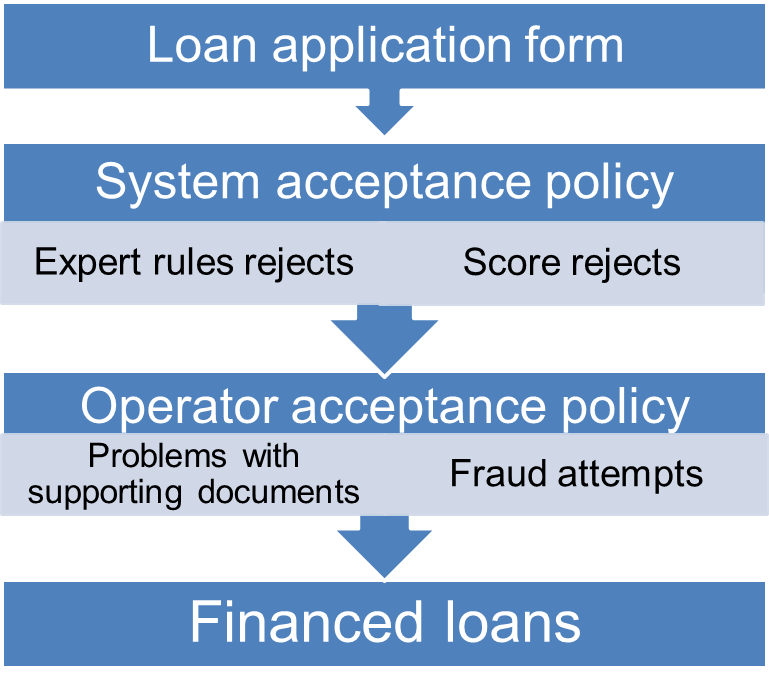
\includegraphics[width=5cm]{figures/schema.png}
\caption{Simplified financing mechanism in~Crédit Agricole Consumer Finance}
\label{fig:figure1}

\end{minipage}%
\hfil \begin{minipage}[c]{0.5\linewidth}

\center 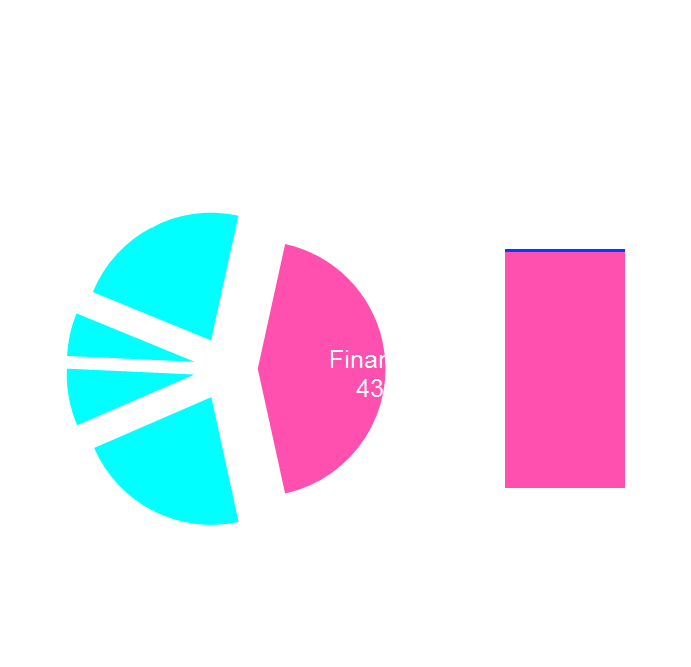
\includegraphics[width=5cm]{figures/camembert_invert.png}
\caption{Proportion of ``final'' lending decisions for CACF France}

\end{minipage}
\end{figure}

\end{frame}








\begin{frame}
\frametitle{\secname: \subsecname}

%%%%%%%%%%%%%%%%%%%%
\note{Si on revient à la formalisation statistique, on a une contrainte de modélisation par régression logistique, qu'on interprète ici comme un espace des paramètres grand $\theta$ fixe, et une pratique ``métier'' consistant à n'utiliser que les clients financés dans l'estimation de $\theta$ qu'on note $\hat{\bm{\theta}}_{\f}$.

\bigskip

A ce stade, implicitement, le chargé d'études statistiques approche un paramètre asymptotique symbolisé par l'étoile, minimisant une divergence de Kullback-Leibler entre la vraie loi et la loi logistique conditionnellement à Z=f, c-à-d au fait d'être financé.}
%%%%%%%%%%%%%%%%%%%%




The industry traditionally fits a $\underbrace{\text{logistic regression}}_{\text{modelling constraint}}$ using only $\underbrace{\text{financed clients}}_{\substack{\text{convenience and lack} \\ \text{of better procedure}}}$ ({\bf fixed parameter space $\Theta$}):

\begin{minipage}[c]{0.1\linewidth}
\begin{animateinline}[poster=first,loop]{2}%
{\color{orange}{\bf CACF}}%
\newframe \end{animateinline}
\end{minipage}
\begin{minipage}[c]{0.85\linewidth}
\[ \hat{\bm{\theta}}_{\f} = \argmax_{\bm{\theta}} \ell(\bm{\theta} ; \mathcal{T}_\f) = \sum_{i=1}^n \ln p_{\bm{\theta}}(y_i | \bm{x}_i), \]
\end{minipage}
which asymptotically approximates:
\[ \bm{\theta}_{\f}^\star = \argmin_{\bm{\theta}} \mathbb{E}_{\bm{X}} [\text{KL}(p || p_{\bm{\theta}}) | \textcolor{green}{Z = \f}]. \]

\end{frame}





\begin{frame}
\frametitle{\secname: \subsecname}


%%%%%%%%%%%%%%%%%%%%%%%%
\note{Ce qu'on aimerait avoir plutôt, c'est le paramètre $\bm{\theta}^\star$ qui n'est pas conditionnel au fait d'être financé et qui pourrait être très simplement obtenu comme une quantité asymptotique du paramètre de maximum de vraisemblance $\hat{\bm{\theta}}$ irrémédiablement inaccessible puisqu'on ne connaît pas toutes les étiquettes.

D'un point de vue géométrique, on peut représenter l'espace des modèles de regression logistique de coefficient $\theta$, la vraie loi qui n'est pas forcément dans cet espace, le paramètre $\bm{\theta}^\star$ qui est la projection orthogonale de cette loi sur l'espace du modèle et le paramètre conditionnel au financement qui se promène dans cet espace et dont le biais est potentiellement plus grand que $\bm{\theta}^\star$.

C'est là tout l'enjeu d'une formalisation rigoureuse : montrer sous quelles hypothèses ce biais existe et si ces hypothèses sont réalistes.

Notons aussi que même à supposer que les paramètres asymptotiques sont égaux, la variance du paramètre conditionnel au fait d'être financé sera plus grande puisqu'on a moins d'observations.}
%%%%%%%%%%%%%%%%%%%%%%%%



Oracle to be approximated:
\begin{align*}
\bm{\theta}^\star & = \argmin_{\bm{\theta}} \mathbb{E}_{\bm{X}} [\text{KL}(p || p_{\bm{\theta}})] \\
& = \argmax_{\bm{\theta}} \mathbb{E}_{\bm{x}, y \sim p} [\ln p_{\bm{\theta}}(y | \bm{x})],
\end{align*}
which standard estimator would be:
\[ \hat{\bm{\theta}} = \argmax_{\bm{\theta}} \ell(\bm{\theta} ; \mathcal{T}_{\text{c}}), \]
but we lack $\mathbf{y}_{\nf}$.
\mode<beamer> {
\vspace*{-0.8cm}
\begin{center}
\resizebox{0.8\textwidth}{4.7cm}{
\begin{tikzpicture}[scale=1.1,every node/.style={minimum size=1cm},on grid]

	% Real level
	\begin{scope}[
		yshift=-120,
		every node/.append style={yslant=\yslant,xslant=\xslant},
		yslant=\yslant,xslant=\xslant
	] 
		% The frame:
		\draw[white, dashed, thin] (0,0) rectangle (7,7); 
		% Agents:
		\draw[fill=orange]  
			(5,2) circle (.1) % Firms
			(2,2) circle (.1); % Households
		% Flows:
		\draw[-latex,thin, yellow] 
			(2,2.2) to (2,4); % Labour Powers
		\draw[-latex,thin, yellow]
			(4.85,1.85) to (4,1); % Wages
		 % Labels:
		\fill[white]
			(0.5,6.5) node[right, scale=2.5] {Model space $\Theta$}	
			(4.9,1.9) node[right,scale=2]{$\theta_{\f}^\star$}
			(2.1,1.9) node[below,scale=2]{$\theta^\star$}
			(2.2,4.3) node [scale=2] {$\hat{\theta}$} 
			(4.2,0.6) node [scale=2] {$\hat{\theta}_{\f}$};
		\fill[yellow]
			(1,3) node [scale=1] {Estimation}
            (1,2.7) node [scale=1] {bias+variance};
		\fill[yellow]
			(5.7,1.1) node [scale=1] {Estimation}
            (5.7,0.8) node [scale=1] {bias+variance};

	\end{scope}
	
	% 2 vertical lines for linking agents on the 2 levels
	\draw[thin, dashed, orange](.8,1.75) to (3.8,-0.32);
	\draw[thin, dashed, orange](.8,1.75) to (.8,-1.8);
	
    % Draw right angle scheme
    \draw(.8,-1.6) to (1,-1.6);
    \draw(1,-1.6) to (1,-1.8);


	% Monetary level
	\begin{scope}[
		yshift=-20,
		every node/.append style={yslant=0,xslant=0},
		yslant=\yslant,xslant=\xslant
	]
		 % Agents:
		\draw [fill=green]
			(2,2) circle (.1); % Households
		 % Labels:
		\fill[black]
			(2.2,2.4) node[right,scale=2]{\textcolor{green}{$p(y|\bm{x})$}};
%			(4,2) node[right,scale=2]{\textcolor{olive}{$p(y|\bm{x}, z = \f)$}};
        \fill[orange]
			(0.85,0.35) node [right, scale=1.5] {Model bias};	

	\end{scope} 
\end{tikzpicture}
}
\end{center}
}

\mode<handout> {

\vspace*{-0.8cm}
\begin{center}
\resizebox{0.8\textwidth}{4.7cm}{
\begin{tikzpicture}[scale=1.1,every node/.style={minimum size=1cm},on grid]

	% Real level
	\begin{scope}[
		yshift=-120,
		every node/.append style={yslant=\yslant,xslant=\xslant},
		yslant=\yslant,xslant=\xslant
	] 
		% The frame:
		\draw[black, dashed, thin] (0,0) rectangle (7,7); 
		% Agents:
		\draw[fill=orange]  
			(5,2) circle (.1) % Firms
			(2,2) circle (.1); % Households
		% Flows:
		\draw[-latex,thin, blue] 
			(2,2.2) to (2,4); % Labour Powers
		\draw[-latex,thin, blue]
			(4.85,1.85) to (4,1); % Wages
		 % Labels:
		\fill[black]
			(0.5,6.5) node[right, scale=2.5] {Model space $\Theta$}	
			(4.9,1.9) node[right,scale=2]{$\theta_{\f}^\star$}
			(2.1,1.9) node[below,scale=2]{$\theta^\star$}
			(2.2,4.3) node [scale=2] {$\hat{\theta}$} 
			(4.2,0.6) node [scale=2] {$\hat{\theta}_{\f}$};
		\fill[blue]
			(1,3) node [scale=1] {Estimation}
            (1,2.7) node [scale=1] {bias+variance};
		\fill[blue]
			(5.7,1.1) node [scale=1] {Estimation}
            (5.7,0.8) node [scale=1] {bias+variance};

	\end{scope}
	
	% 2 vertical lines for linking agents on the 2 levels
	\draw[thin, dashed, orange](.8,1.75) to (3.8,-0.32);
	\draw[thin, dashed, orange](.8,1.75) to (.8,-1.8);
	
    % Draw right angle scheme
    \draw(.8,-1.6) to (1,-1.6);
    \draw(1,-1.6) to (1,-1.8);


	% Monetary level
	\begin{scope}[
		yshift=-20,
		every node/.append style={yslant=0,xslant=0},
		yslant=\yslant,xslant=\xslant
	]
		 % Agents:
		\draw [fill=green]
			(2,2) circle (.1); % Households
		 % Labels:
		\fill[black]
			(2.2,2.4) node[right,scale=2]{\textcolor{green}{$p(y|\bm{x})$}};
%			(4,2) node[right,scale=2]{\textcolor{olive}{$p(y|\bm{x}, z = \f)$}};
        \fill[orange]
			(0.85,0.35) node [right, scale=1.5] {Model bias};	

	\end{scope} 
\end{tikzpicture}
}
\end{center}
}

\end{frame}



\subsection{modelling the financing mechanism}

\begin{frame}
\frametitle{\secname : \subsecname}



%%%%%%%%%%%%%%
\note{
Principal apport de la thèse : formalisation

Interprétation comme un problème à données manquantes

Cadre statistique standard
}
%%%%%%%%%%%%%%

\begin{minipage}[c]{0.1\textwidth}
\begin{animateinline}[poster=first,loop]{2}%
{\color{orange}{\bf CACF}}%
\newframe \end{animateinline}
\end{minipage}
\begin{minipage}[c]{0.85\textwidth}
Due to the financing mechanism, labels $y$ are not MCAR.
\end{minipage}

\medskip

%\uncover<2->{
\begin{minipage}[c]{0.2\textwidth}
\begin{animateinline}[poster=first,loop]{2}%
{\color{orange}{\bf Statistician}}%
\newframe \end{animateinline}
\end{minipage}
\begin{minipage}[c]{0.75\textwidth}
Let $\{p_{\bm{\phi}}(z | \bm{x}, y)\}_{\bm{\phi} \in \bm{\Phi}}$ denote this hidden financing mechanism (as a parametrized family).
\end{minipage}
%}

\medskip

\uncover<2->{
Combining financing and credit-worthiness probability distributions:
\[ p_{\bm{\gamma}}(y,z | \bm{x}) = \underbrace{p_{\bm{\theta}(\bm{\gamma})}(y | \bm{x})}_{\text{CACF}} \underbrace{p_{\bm{\phi}(\bm{\gamma})}(z | \bm{x}, y)}_{\text{?}}. \]
}

%\medskip

\uncover<3->{
To estimate $\bm{\gamma}$, we could rely on Maximum Likelihood theory:
}

\uncover<4->{
%\begin{minipage}[c]{0.15\linewidth}
%\only<4->{
%\begin{animateinline}[poster=first,loop]{2}%
%{\color{orange}{\bf Statistician}}%
%\newframe \end{animateinline}}
%\end{minipage}%
%\begin{minipage}[c]{0.80\linewidth}
%\vspace*{-0.6cm}
%\hspace*{0.7cm}
\[ \ell(\bm{\gamma}; \mathcal{T}) = \sum_{i = 1}^n \ln p_{\bm{\gamma}}(y_i,\f | \bm{x}_i) + \sum_{i=n+1}^{n+n'} \ln \sum_{y \in \{0,1\}} p_{\bm{\gamma}}(y,\nf | \bm{x}_i). \]
%\end{minipage}
}

\end{frame}



\begin{frame}
\frametitle{\secname : \subsecname}



%%%%%%%%%%%%%%
\note{

Justifier l’écriture d’EM car on va revoir ça dans des méthodes de réintégration

\bigskip

L'algorithme (S)EM est au coeur de la thèse car aussi utilisé pour la quantification qu'on peut considérer comme des données manquantes et les arbres de régression logistique où la structure d'arbre est manquante

}
%%%%%%%%%%%%%%

%\textit{e.g.}\ \textit{via} an EM algorithm:

%\uncover<2->{
{E\footcite{dempster1977maximum}-step}: compute the \textcolor{green}{conditional probabilities of missing $y_i$ values}:
\begin{equation*}
t_{iy}^{(s)} = p_{\bm{\theta}(\gamma^{(s-1)})}(y|\bm{x}_i,\nf) = \frac{p_{\gamma^{(s-1)}}(y, \nf|\bm{x}_i)}{\sum_{y' = 0}^{1} p_{\gamma^{(s-1)}}(y', \nf|\bm{x}_i)};
\end{equation*}
%}
\uncover<2->{
{M\footnotemark[1]-step}: \textcolor{green}{maximize the conditional expectation} of $\ell_c(\gamma;\mathcal{T}_{\text{c}})$:
\begin{equation*}\label{eq:like.c}
\ell_c(\gamma;\mathcal{T}_{\text{c}}) = \sum_{i=1}^{n+n'}\ln p_{\gamma}(y_i,z_i | \bm{x}_i) = \sum_{i=1}^{n}\ln p_{\gamma}(y_i,\text{f} | \bm{x}_i) + \sum_{i=n+1}^{n+n'}\ln p_{\gamma}(y_i,\text{nf} | \bm{x}_i);
\end{equation*}
%leading to:
\begin{align*}
\gamma^{(s)} & = \argmax_{\gamma \in \Gamma} \mathbb{E}_{\bm{\mathbf{y}}_{\text{nf}}} [\ell_c(\gamma;\mathcal{T}_{\text{c}}) | \mathcal{T},\gamma^{(s-1)}] \\
& = \argmax_{\gamma \in \Gamma} \sum_{i = 1}^n \ln p_{\gamma}(y_i, \f|\bm{x}_i) +  \sum_{i' = n+1}^{n+n'}\sum_{y = 0}^{1}t_{i'y}^{(s)} \ln p_{\gamma}(y, \nf | \bm{x}_{i'}).
\end{align*}
}
\end{frame}




\subsection{flawed model selection}

\begin{frame}
\frametitle{\secname : \subsecname}



%%%%%%%%%%%
\note{

Soit investissement statistique : modélisation additionnelle

Soit investissement financier supplémentaire : payer pour voir

Aucun des deux
}
%%%%%%%%%%%

No free dinner: \textcolor{green}{financial or statistical investment to make}.

\vspace*{0.2cm}

\begin{minipage}[c]{0.1\textwidth}
\begin{animateinline}[poster=first,loop]{2}%
{\color{orange}{\bf CACF}}%
\newframe \end{animateinline}
\end{minipage}
\begin{minipage}[c]{0.85\textwidth}
Because no test-sample $\mathcal{T}^{\text{test}}$ is available $\underbrace{\text{from } p(\bm{x}, y)}_{\substack{\cancel{\text{funding bad clients}} \\ \cancel{\text{at a loss}}}}$, 
\vspace*{-0.8cm}

we cannot resort to error-rate criteria:
\end{minipage}

\[ \mbox{Error}(\mathcal{T}^\text{test}) = \frac{1}{|\mathcal{T}^\text{test}|} \sum_{i \in \mathcal{T}^\text{test}} \mathbb{I}(\hat y_i \neq y_i). \]

%\vspace*{1cm}

\medskip

\uncover<2->{
We should use information criteria on the observed data $\mathcal{T}$ such as:
%\begin{minipage}[c]{0.15\textwidth}
%\begin{animateinline}[poster=last, loop]{2}%
%{\color{orange}{\bf Statistician}}%
%\newframe \end{animateinline}
%\end{minipage}
%\begin{minipage}[c]{0.80\textwidth}
\[ \text{BIC}(\hat{\bm{\gamma}};\mathcal{T}) = -2 \ell(\hat{\bm{\gamma}}; \mathcal{T}) + \text{dim}(\bm{\Gamma})\ln n, \]
%\vspace*{0.0cm}
%\end{minipage}
where $\hat{\bm{\gamma}} = \argmax_{\bm{\gamma}} \ell(\bm{\gamma}; \mathcal{T})$, to compare models.
}

\medskip

\uncover<3->{
%\begin{minipage}[c]{0.1\textwidth}
%\begin{animateinline}[poster=last, loop]{2}%
%{\color{orange}{\bf CACF}}%
%\newframe \end{animateinline}
%\end{minipage}
%\begin{minipage}[c]{0.85\textwidth}
It requires to precisely state the models $\{ p_{\bm{\gamma}}(y,z | \bm{x})\}_{\bm{\Gamma}}$ that compete and their underlying assumptions.
%: logistic regression constraint + additional modelling steps.
%\end{minipage}
}

\end{frame}






\subsection{strategies}

\begin{frame}
\frametitle{\secname : \subsecname}



%%%%%%%%%%%%%%%%
\note{
Les méthodes sont proches de la formalisation introduite précédemment mais nécessitaient une prise de recul scientifique. Exemple.

}
%%%%%%%%%%%%%%%%




We gathered 6 so-called Reject Inference methods from the literature
%~\cite{economix,saporta,RI6,banasik} 
that aim at re-injecting $\bm{\mathbf{x}}_{\nf}$ into the estimation procedure of $\bm{\theta}$.

\medskip

They usually resemble EM-like algorithms:

{
\setbeamercolor{normal text}{fg=black}
\usebeamercolor[fg]{normal text}

\[ \hspace*{-0.8cm}\textcolor{white}{\mathcal{T}_{\text{c}}^{(1)} = {\Huge \Bigg(}}
%\begin{array}{c}
%\tikzmarkin[hor=style green]{el0} \mathbf{x}_{\f} \tikzmarkend{el0} \\
%\\
%\\
%\tikzmarkin[hor=style green]{el-1} \mathbf{x}_{\nf} \tikzmarkend{el-1} \end{array}
\textcolor{white}{{\Huge \Bigg(}}
\begin{array}{ccc}
\tikzmarkin[hor=style green]{el1} \; \; x_{1,1} & \cdots & x_{1,d}  \\
 \vdots & \vdots & \vdots \\
 x_{n,1} & \cdots & x_{n,d} \\
 x_{n+1,1} & \cdots & x_{n+1,d}  \\
 \vdots & \vdots & \vdots \\
 x_{n+n',1} & \cdots & x_{n+n',d} \tikzmarkend{el1} \end{array} \textcolor{white}{{\Huge \Bigg)},}
 %\hspace{0.2cm}
% \begin{array}{c}
%\tikzmarkin[hor=style green]{l1} \mathbf{y}_{\f} \tikzmarkend{l1}\\
%\\
%\\
%\tikzmarkin[hor=style green]{l2} \mathbf{y}_{\nf} \tikzmarkend{l2} \end{array}
\textcolor{white}{{\Huge \Bigg(}}
\begin{array}{c}
\tikzmarkin[hor=style green]{l3} \; \; y_1 \; \; \; \\
\vdots \\
 y_n \\ 
 \hat{y}_{n+1}^{(1)} \\
\vdots \\
\hat{y}_{n+n'}^{(1)} \tikzmarkend{l3}\end{array} \textcolor{white}{{\Huge \Bigg)},}
%\hspace{0.2cm} 
% \begin{array}{c}
%\tikzmarkin[hor=style green]{el111} \mathbf{z}_{\f} \tikzmarkend{el111}\\
%\\
%\\
%\tikzmarkin[hor=style green]{el121} \mathbf{z}_{\nf} \tikzmarkend{el121}\end{array}
\textcolor{white}{{\Huge \Bigg(}}
\begin{array}{c}
\tikzmarkin[hor=style green]{e41} \text{f} \\
\vdots \\
\text{f} \\ 
\text{nf} \\
\vdots \\
\text{nf} \tikzmarkend{e41} \end{array} \textcolor{white}{{\Huge \Bigg) \Bigg)}}\]
 }
 
%\setbeamercolor{normal text}{fg=white}
%\usebeamercolor[fg]{normal text}

Can we \textcolor{green}{reinterpret these empirical methods} in the missing data and information criterion frameworks and / or expose their \textcolor{green}{implicit modelling} steps?

\end{frame}





\subsection{example of Fuzzy Augmentation\footcite{economix}}

\begin{frame}
\frametitle{\secname : \subsecname}



%%%%%%%%%%%%%%%%
\note{
On commence par l'estimation de $\hat{\bm{\theta}}_\f$ comme la méthode traditionnelle.

On estime la probabilité de l'évènement sur les clients financés qu'on substitue pour leur label.

On recommence l'estimation sur l'échantillon ainsi complété.

Or le lieu du maximum de vraisemblance des non financés est le même que les financés : ça revient en régression à rajouter des points sur la droite de régression estimée : ça ne fait qu'augmenter artificiellement le R2.

On retombe donc sur le coefficient de départ.
}
%%%%%%%%%%%%%%%%

Estimate $\hat{\bm{\theta}}_\f = \argmax_{\bm{\theta}} \ell(\bm{\theta};\mathcal{T}_\f)$, infer for $n+1 \leq i \leq n + n'$:
\[ \textcolor{green}{\hat{y}_i = p_{\hat{\bm{\theta}}_\f}(1| \bm{x}_i)}, \]

\uncover<2->{
and re-estimate $\bm{\theta}$ using the resulting $\mathcal{T}_{\text{c}}$. For $1 \leq j \leq d$:

\[ \frac{\partial \sum_{i=n+1}^{n'+n} \sum_{y_i = 0}^{1} p_{\hat{\bm{\theta}}_\f}(y_i| \bm{x}_i)\ln (p_{\bm{\theta}}(y_i| \bm{x}_i))}{\partial \theta_j} = 0 \Leftrightarrow \bm{\theta} = \hat{\bm{\theta}}_{\f}, \]
}

\uncover<3->{
such that:
\[\argmax_{\bm{\theta} \in \Theta}  \sum_{i=n+1}^{n'+n} \sum_{y_i = 0}^{1} p_{\hat{\bm{\theta}}_{\f}}(y_i| \bm{x}_i)\ln (p_{\bm{\theta}}(y_i| \bm{x}_i)) = \hat{\bm{\theta}}_{\f}.\]
}

\uncover<4->{
Finally:
\[\argmax_{\bm{\theta} \in \Theta} \ell(\bm{\theta};\mathcal{T}_{c}) = \argmax_{\bm{\theta} \in \Theta} \ell(\bm{\theta};\mathcal{T}_\f) = \hat{\bm{\theta}}_{\f}. \]
}

\end{frame}





\subsection{missingness mechanism}

\begin{frame}
\frametitle{\secname : \subsecname}


%%%%%%%%%%%%%%%
\note{

Strictement parlant, on est MNAR dans le cas CACF, mais probablement pas loin de MAR car automatisation prépondérante, mais pas testable.
}
%%%%%%%%%%%%%%%



\begin{itemize}
%\item \textbf{Ignorability}\footcite{littlerubin}: no functional dependence between $\bm{\theta}$ and $\bm{\phi}$, \textit{e.g.}\ $\bm{\gamma} = (\bm{\theta},\bm{\phi})$.

\item<1-> \textbf{MAR}\footcite{littlerubin}: $\forall \: \bm{x},y,z, \; p(z| \bm{x},y) = p(z| \bm{x})$

$\rightarrow$ Financing is determined by an old score: $Z = \mathds{1}_{\{(1,\bm{x})'\bm{\theta} > \text{cut}\}}$.

\item<2-> \textbf{MNAR}\footnotemark[3]: $\exists \: \bm{x},y,z, \; p(z| \bm{x},y) \neq p(z| \bm{x})$

$\rightarrow$ Operators' hidden ``feeling'' $\tilde{\bm{X}}$ influence the financing.

$\rightarrow$ Expert rules based on both present and hidden features $\bm{X}$ and $\tilde{\bm{X}}$ resp.\ where $\tilde{\bm{X}}$ cannot be totally explained by $\bm{X}$.

$\rightarrow$ Cannot be tested \footcite{molenberghs2008every}.
\end{itemize}

\uncover<3->{
\begin{figure}
\begin{tikzpicture}[scale=0.8]

\tikzset{vertex/.style = {shape=circle,draw,minimum size=1.5em}}
\tikzset{edge/.style = {->,> = latex'}}
% vertices
\node[vertex] (y) at  (0,0) {$Y$};
\node[vertex] (x) at  (2,-1) {$\bm{X}$};
\node[vertex] (xc) at  (2,1) {$\tilde{\bm{X}}$};
\node[vertex] (z) at (4,0) {$Z$};

edges
\draw[edge] (y) to (x);
\draw[edge] (y) to (xc);
\draw[dashed] (xc) to (x);
\draw[edge] (xc) to (z);
\draw[edge] (x) to (z);

\end{tikzpicture}
%\label{fig:mar}
%\caption{Dependencies between random variables $Y$, $\bm{\tilde{X}}$, $\bm{X}$ and $Z$}
\end{figure}
}
\end{frame}






\subsection{research contribution}

\begin{frame}
\frametitle{\secname : \subsecname}


%%%%%%%%%%%%%%%%
\note{
Une autre méthode conduit au même coefficient : Twins.

\medskip

La méthode dite Reclassification est équivalente à un Classification-EM, c'est-à-dire la même chose que l'EM de la slide précédente mais avec une affectation dure à bon ou mauvais en fonction d'un seuil sur la probabilité. On peut montrer que cela induit un biais sur l'estimation de $\bm{\theta}$.

\medskip

On peut ensuite distinguer les cas MAR et MNAR d'un côté et le bon modèle : la vraie loi appartient à l'espace du modèle ou mauvais modèle.

\medskip

Importance Sampling : demande modélisation du mécanisme de financement.

\medskip

MNAR: modélisation + hypothèses invérifiables obligatoires.
}
%%%%%%%%%%%%%%%%




Fuzzy Augmentation and Twins produce \textcolor{green}{the same coefficient $\hat{\bm{\theta}}_{\text{f}}$}.

\medskip

Reclassification\footcite{saporta}$^{,}$\footcite{RI6}$^{,}$\footcite{banasik} is equivalent to a Classification-EM algorithm, thus introducing a \textcolor{green}{bias} in the estimation of $\bm{\theta}$.

\vspace*{-0.7cm}
\begin{table}
%\caption{Summary of potential biases.}
%\begin{center}
\hspace*{-0.6cm}
\begin{tabular}{L{2.2cm} | C{4.5cm} | C{4cm}}
 & MAR & MNAR \\
 \hline
 Well-specified model & $\hat{\bm{\theta}}_{\text{f}}$ is unbiased. & \multirowcell{2}{$\hat{\bm{\theta}}_{\text{f}}$ is biased.\\ Any correction  relies \\ on \textit{a priori} \textcolor{green}{unverifiable} \\ \textcolor{green}{assumptions} about \\ $p_{\bm{\phi}}(z | \bm{x}, y)$, \textit{e.g.}\ the \\ Parcelling\footnotemark[5]$^{,}$\footnotemark[6]$^{,}$\footnotemark[7] method.} \\
 \cline{1-2}
 Misspecified model & $\hat{\bm{\theta}}_{\text{f}}$ is biased: Augmentation\footnotemark[2]$^{,}$\footnotemark[5]$^{,}$\footnotemark[6]$^{,}$\footnotemark[7] could be suitable but introduces a \textcolor{green}{new estimation} procedure\footcite{zadrozny2004learning} {\footnotesize (which requires $\forall \bm{x}, p(\f | \bm{x}) > 0$)}. & \\
\end{tabular}
%\end{center}
\end{table}
\vspace*{-0.2cm}

\end{frame}



\subsection{industry contribution}

\begin{frame}
\frametitle{\secname : \subsecname}



%%%%%%%%%%%%%%%%
\note{On retourne au cadre CACF où on teste ces trois méthodes sur deux jeux de données : un portefeuille d'un partenaire de grande distribution et un portefeuille compte propre, c-à-d Sofinco

\bigskip

Dans les deux cas, on simule artificiellement un mécanisme de rejet en augmentant progressivement le cut de l'ancien score, jusqu'au point où il n'y a plus suffisamment de mauvais payeur pour apprendre.

\bigskip

On a ainsi une sorte d'ensemble test de $p(x,y,z)$.

\bigskip

On remarque que les trois méthodes ne sont pas significativement différentes en termes de Gini.

\bigskip

Notre conseil à CACF est donc de ne pas pratiquer de réintégration dans le cas de la régression logistique.
}
%%%%%%%%%%%%%%%%


\mode<beamer>{
\vspace*{-1cm}
\begin{figure}[!ht]
\centering \resizebox{\textwidth}{!}{% Created by tikzDevice version 0.12 on 2019-06-13 15:42:19
% !TEX encoding = UTF-8 Unicode
\begin{tikzpicture}[x=1pt,y=1pt, scale=0.6]
\definecolor{fillColor}{RGB}{255,255,255}
\path[use as bounding box,fill=fillColor,fill opacity=0.00] (0,0) rectangle (578.16,231.26);
\begin{scope}
\path[clip] ( 49.20, 61.20) rectangle (552.96,182.06);
\definecolor{drawColor}{RGB}{255,255,255}

\path[draw=drawColor,line width= 1.2pt,line join=round,line cap=round] ( 67.86,176.85) --
	( 67.90,176.85) --
	( 67.90,176.85) --
	(108.35,176.26) --
	(122.20,177.56) --
	(201.20,177.59) --
	(291.41,156.62) --
	(349.16,151.14) --
	(432.12,114.79) --
	(518.48, 65.68);
\definecolor{fillColor}{RGB}{255,255,255}

\path[fill=fillColor] ( 65.61,174.60) --
	( 70.11,174.60) --
	( 70.11,179.10) --
	( 65.61,179.10) --
	cycle;

\path[fill=fillColor] ( 65.65,174.60) --
	( 70.15,174.60) --
	( 70.15,179.10) --
	( 65.65,179.10) --
	cycle;

\path[fill=fillColor] ( 65.65,174.60) --
	( 70.15,174.60) --
	( 70.15,179.10) --
	( 65.65,179.10) --
	cycle;

\path[fill=fillColor] (106.10,174.01) --
	(110.60,174.01) --
	(110.60,178.51) --
	(106.10,178.51) --
	cycle;

\path[fill=fillColor] (119.95,175.31) --
	(124.45,175.31) --
	(124.45,179.81) --
	(119.95,179.81) --
	cycle;

\path[fill=fillColor] (198.95,175.34) --
	(203.45,175.34) --
	(203.45,179.84) --
	(198.95,179.84) --
	cycle;

\path[fill=fillColor] (289.16,154.37) --
	(293.66,154.37) --
	(293.66,158.87) --
	(289.16,158.87) --
	cycle;

\path[fill=fillColor] (346.91,148.89) --
	(351.41,148.89) --
	(351.41,153.39) --
	(346.91,153.39) --
	cycle;

\path[fill=fillColor] (429.87,112.54) --
	(434.37,112.54) --
	(434.37,117.04) --
	(429.87,117.04) --
	cycle;

\path[fill=fillColor] (516.23, 63.43) --
	(520.73, 63.43) --
	(520.73, 67.93) --
	(516.23, 67.93) --
	cycle;
\end{scope}
\begin{scope}
\path[clip] (  0.00,  0.00) rectangle (578.16,231.26);
\definecolor{drawColor}{RGB}{255,255,255}

\path[draw=drawColor,line width= 1.2pt,line join=round,line cap=round] ( 49.20, 61.20) --
	(552.96, 61.20) --
	(552.96,182.06) --
	( 49.20,182.06) --
	( 49.20, 61.20);
\end{scope}
\begin{scope}
\path[clip] (  0.00,  0.00) rectangle (578.16,231.26);
\definecolor{drawColor}{RGB}{255,255,255}

\node[text=drawColor,anchor=base,inner sep=0pt, outer sep=0pt, scale=  1.00] at (301.08, 15.60) {Acceptance rate};

\node[text=drawColor,rotate= 90.00,anchor=base,inner sep=0pt, outer sep=0pt, scale=  1.00] at ( 10.80,121.63) {Gini on test set};
\end{scope}
\begin{scope}
\path[clip] ( 49.20, 61.20) rectangle (552.96,182.06);
\definecolor{drawColor}{RGB}{255,165,0}

\path[draw=drawColor,line width= 1.2pt,dash pattern=on 1pt off 3pt ,line join=round,line cap=round] ( 67.86,177.22) --
	( 67.90,177.22) --
	( 67.90,177.22) --
	(108.35,175.71) --
	(122.20,176.52) --
	(201.20,177.59) --
	(291.41,152.44) --
	(349.16,151.70) --
	(432.12,116.95) --
	(518.48, 65.68);
\definecolor{fillColor}{RGB}{255,165,0}

\path[fill=fillColor] ( 67.86,180.72) --
	( 70.89,175.48) --
	( 64.83,175.48) --
	cycle;

\path[fill=fillColor] ( 67.90,180.72) --
	( 70.93,175.48) --
	( 64.87,175.48) --
	cycle;

\path[fill=fillColor] ( 67.90,180.72) --
	( 70.93,175.48) --
	( 64.87,175.48) --
	cycle;

\path[fill=fillColor] (108.35,179.21) --
	(111.38,173.96) --
	(105.32,173.96) --
	cycle;

\path[fill=fillColor] (122.20,180.02) --
	(125.23,174.77) --
	(119.17,174.77) --
	cycle;

\path[fill=fillColor] (201.20,181.09) --
	(204.23,175.84) --
	(198.17,175.84) --
	cycle;

\path[fill=fillColor] (291.41,155.94) --
	(294.45,150.69) --
	(288.38,150.69) --
	cycle;

\path[fill=fillColor] (349.16,155.20) --
	(352.19,149.95) --
	(346.13,149.95) --
	cycle;

\path[fill=fillColor] (432.12,120.45) --
	(435.15,115.20) --
	(429.09,115.20) --
	cycle;

\path[fill=fillColor] (518.48, 69.18) --
	(521.51, 63.93) --
	(515.45, 63.93) --
	cycle;
\end{scope}
\begin{scope}
\path[clip] (  0.00,  0.00) rectangle (578.16,231.26);
\definecolor{drawColor}{RGB}{255,255,255}

\path[draw=drawColor,line width= 1.2pt,line join=round,line cap=round] ( 49.20, 61.20) --
	(552.96, 61.20) --
	(552.96,182.06) --
	( 49.20,182.06) --
	( 49.20, 61.20);
\end{scope}
\begin{scope}
\path[clip] (  0.00,  0.00) rectangle (578.16,231.26);
\definecolor{drawColor}{RGB}{255,255,255}

\node[text=drawColor,anchor=base,inner sep=0pt, outer sep=0pt, scale=  1.00] at (301.08, 15.60) {Acceptance rate};

\node[text=drawColor,rotate= 90.00,anchor=base,inner sep=0pt, outer sep=0pt, scale=  1.00] at ( 10.80,121.63) {Gini on test set};
\end{scope}
\begin{scope}
\path[clip] ( 49.20, 61.20) rectangle (552.96,182.06);
\definecolor{drawColor}{RGB}{255,0,255}

\path[draw=drawColor,line width= 1.2pt,dash pattern=on 1pt off 3pt on 4pt off 3pt ,line join=round,line cap=round] ( 67.86,177.59) --
	( 67.90,177.59) --
	( 67.90,177.59) --
	(108.35,176.27) --
	(122.20,176.39) --
	(201.20,176.36) --
	(291.41,156.29) --
	(349.16,162.21) --
	(432.12,108.61) --
	(518.48, 65.68);

\path[draw=drawColor,line width= 1.2pt,line join=round,line cap=round] ( 65.61,175.34) -- ( 70.11,179.84);

\path[draw=drawColor,line width= 1.2pt,line join=round,line cap=round] ( 65.61,179.84) -- ( 70.11,175.34);

\path[draw=drawColor,line width= 1.2pt,line join=round,line cap=round] ( 64.68,177.59) -- ( 71.04,177.59);

\path[draw=drawColor,line width= 1.2pt,line join=round,line cap=round] ( 67.86,174.41) -- ( 67.86,180.77);

\path[draw=drawColor,line width= 1.2pt,line join=round,line cap=round] ( 65.65,175.34) -- ( 70.15,179.84);

\path[draw=drawColor,line width= 1.2pt,line join=round,line cap=round] ( 65.65,179.84) -- ( 70.15,175.34);

\path[draw=drawColor,line width= 1.2pt,line join=round,line cap=round] ( 64.71,177.59) -- ( 71.08,177.59);

\path[draw=drawColor,line width= 1.2pt,line join=round,line cap=round] ( 67.90,174.41) -- ( 67.90,180.77);

\path[draw=drawColor,line width= 1.2pt,line join=round,line cap=round] ( 65.65,175.34) -- ( 70.15,179.84);

\path[draw=drawColor,line width= 1.2pt,line join=round,line cap=round] ( 65.65,179.84) -- ( 70.15,175.34);

\path[draw=drawColor,line width= 1.2pt,line join=round,line cap=round] ( 64.71,177.59) -- ( 71.08,177.59);

\path[draw=drawColor,line width= 1.2pt,line join=round,line cap=round] ( 67.90,174.41) -- ( 67.90,180.77);

\path[draw=drawColor,line width= 1.2pt,line join=round,line cap=round] (106.10,174.02) -- (110.60,178.52);

\path[draw=drawColor,line width= 1.2pt,line join=round,line cap=round] (106.10,178.52) -- (110.60,174.02);

\path[draw=drawColor,line width= 1.2pt,line join=round,line cap=round] (105.17,176.27) -- (111.53,176.27);

\path[draw=drawColor,line width= 1.2pt,line join=round,line cap=round] (108.35,173.09) -- (108.35,179.45);

\path[draw=drawColor,line width= 1.2pt,line join=round,line cap=round] (119.95,174.14) -- (124.45,178.64);

\path[draw=drawColor,line width= 1.2pt,line join=round,line cap=round] (119.95,178.64) -- (124.45,174.14);

\path[draw=drawColor,line width= 1.2pt,line join=round,line cap=round] (119.02,176.39) -- (125.38,176.39);

\path[draw=drawColor,line width= 1.2pt,line join=round,line cap=round] (122.20,173.21) -- (122.20,179.57);

\path[draw=drawColor,line width= 1.2pt,line join=round,line cap=round] (198.95,174.11) -- (203.45,178.61);

\path[draw=drawColor,line width= 1.2pt,line join=round,line cap=round] (198.95,178.61) -- (203.45,174.11);

\path[draw=drawColor,line width= 1.2pt,line join=round,line cap=round] (198.02,176.36) -- (204.38,176.36);

\path[draw=drawColor,line width= 1.2pt,line join=round,line cap=round] (201.20,173.18) -- (201.20,179.54);

\path[draw=drawColor,line width= 1.2pt,line join=round,line cap=round] (289.16,154.04) -- (293.66,158.54);

\path[draw=drawColor,line width= 1.2pt,line join=round,line cap=round] (289.16,158.54) -- (293.66,154.04);

\path[draw=drawColor,line width= 1.2pt,line join=round,line cap=round] (288.23,156.29) -- (294.60,156.29);

\path[draw=drawColor,line width= 1.2pt,line join=round,line cap=round] (291.41,153.11) -- (291.41,159.48);

\path[draw=drawColor,line width= 1.2pt,line join=round,line cap=round] (346.91,159.96) -- (351.41,164.46);

\path[draw=drawColor,line width= 1.2pt,line join=round,line cap=round] (346.91,164.46) -- (351.41,159.96);

\path[draw=drawColor,line width= 1.2pt,line join=round,line cap=round] (345.98,162.21) -- (352.34,162.21);

\path[draw=drawColor,line width= 1.2pt,line join=round,line cap=round] (349.16,159.03) -- (349.16,165.39);

\path[draw=drawColor,line width= 1.2pt,line join=round,line cap=round] (429.87,106.36) -- (434.37,110.86);

\path[draw=drawColor,line width= 1.2pt,line join=round,line cap=round] (429.87,110.86) -- (434.37,106.36);

\path[draw=drawColor,line width= 1.2pt,line join=round,line cap=round] (428.94,108.61) -- (435.31,108.61);

\path[draw=drawColor,line width= 1.2pt,line join=round,line cap=round] (432.12,105.43) -- (432.12,111.79);

\path[draw=drawColor,line width= 1.2pt,line join=round,line cap=round] (516.23, 63.43) -- (520.73, 67.93);

\path[draw=drawColor,line width= 1.2pt,line join=round,line cap=round] (516.23, 67.93) -- (520.73, 63.43);

\path[draw=drawColor,line width= 1.2pt,line join=round,line cap=round] (515.30, 65.68) -- (521.66, 65.68);

\path[draw=drawColor,line width= 1.2pt,line join=round,line cap=round] (518.48, 62.49) -- (518.48, 68.86);
\end{scope}
\begin{scope}
\path[clip] (  0.00,  0.00) rectangle (578.16,231.26);
\definecolor{drawColor}{RGB}{255,255,255}

\path[draw=drawColor,line width= 1.2pt,line join=round,line cap=round] ( 49.20, 61.20) --
	(552.96, 61.20) --
	(552.96,182.06) --
	( 49.20,182.06) --
	( 49.20, 61.20);
\end{scope}
\begin{scope}
\path[clip] (  0.00,  0.00) rectangle (578.16,231.26);
\definecolor{drawColor}{RGB}{255,255,255}

\node[text=drawColor,anchor=base,inner sep=0pt, outer sep=0pt, scale=  1.00] at (301.08, 15.60) {Acceptance rate};

\node[text=drawColor,rotate= 90.00,anchor=base,inner sep=0pt, outer sep=0pt, scale=  1.00] at ( 10.80,121.63) {Gini on test set};
\end{scope}
\begin{scope}
\path[clip] (  0.00,  0.00) rectangle (578.16,231.26);
\definecolor{drawColor}{RGB}{255,255,255}

\path[draw=drawColor,line width= 1.2pt,line join=round,line cap=round] (534.30, 61.20) -- ( 67.86, 61.20);

\path[draw=drawColor,line width= 1.2pt,line join=round,line cap=round] (534.30, 61.20) -- (534.30, 55.20);
\node[text=drawColor,anchor=base east,inner sep=0pt, outer sep=0pt, scale=  1.00] at (550, 45) {60 \%};

\path[draw=drawColor,line width= 1.2pt,line join=round,line cap=round] (417.69, 61.20) -- (417.69, 55.20);
\node[text=drawColor,anchor=base east,inner sep=0pt, outer sep=0pt, scale=  1.00] at (430, 45) {70 \%};

\path[draw=drawColor,line width= 1.2pt,line join=round,line cap=round] (301.08, 61.20) -- (301.08, 55.20);
\node[text=drawColor,anchor=base east,inner sep=0pt, outer sep=0pt, scale=  1.00] at (315, 45) {80 \%};

\path[draw=drawColor,line width= 1.2pt,line join=round,line cap=round] (184.47, 61.20) -- (184.47, 55.20);
\node[text=drawColor,anchor=base east,inner sep=0pt, outer sep=0pt, scale=  1.00] at (200, 45) {90 \%};

\path[draw=drawColor,line width= 1.2pt,line join=round,line cap=round] ( 67.86, 61.20) -- ( 67.86, 55.20);
\node[text=drawColor,anchor=base east,inner sep=0pt, outer sep=0pt, scale=  1.00] at (80, 45) {100 \%};


%\path[draw=drawColor,line width= 1.2pt,line join=round,line cap=round] ( 49.20, 17.92) -- ( 49.20,210.29);

\path[draw=drawColor,line width= 1.2pt,line join=round,line cap=round] ( 49.20, 61.20) -- ( 49.20,182.06);

%\path[draw=drawColor,line width= 1.2pt,line join=round,line cap=round] ( 49.20, 17.92) -- ( 43.20, 17.92);

%\path[draw=drawColor,line width= 1.2pt,line join=round,line cap=round] ( 49.20, 49.98) -- ( 43.20, 49.98);

\path[draw=drawColor,line width= 1.2pt,line join=round,line cap=round] ( 49.20, 82.04) -- ( 43.20, 82.04);

\path[draw=drawColor,line width= 1.2pt,line join=round,line cap=round] ( 49.20,114.10) -- ( 43.20,114.10);

\path[draw=drawColor,line width= 1.2pt,line join=round,line cap=round] ( 49.20,146.17) -- ( 43.20,146.17);

\path[draw=drawColor,line width= 1.2pt,line join=round,line cap=round] ( 49.20,178.23) -- ( 43.20,178.23);

%\path[draw=drawColor,line width= 1.2pt,line join=round,line cap=round] ( 49.20,210.29) -- ( 43.20,210.29);

%\node[text=drawColor,anchor=base east,inner sep=0pt, outer sep=0pt, scale=  1.00] at ( 37.20, 14.47) {-10};

%\node[text=drawColor,anchor=base east,inner sep=0pt, outer sep=0pt, scale=  1.00] at ( 37.20, 46.54) {0};

\node[text=drawColor,anchor=base east,inner sep=0pt, outer sep=0pt, scale=  1.00] at ( 37.20, 78.60) {10};

\node[text=drawColor,anchor=base east,inner sep=0pt, outer sep=0pt, scale=  1.00] at ( 37.20,110.66) {20};

\node[text=drawColor,anchor=base east,inner sep=0pt, outer sep=0pt, scale=  1.00] at ( 37.20,142.72) {30};

\node[text=drawColor,anchor=base east,inner sep=0pt, outer sep=0pt, scale=  1.00] at ( 37.20,174.79) {40};

%\node[text=drawColor,anchor=base east,inner sep=0pt, outer sep=0pt, scale=  1.00] at ( 37.20,206.85) {50};

\path[draw=drawColor,line width= 1.2pt,line join=round,line cap=round] ( 67.86,155.79) rectangle (180.16,119.79);

\path[draw=drawColor,line width= 1.2pt,line join=round,line cap=round] ( 69.88,146.79) -- ( 83.38,146.79);
\definecolor{drawColor}{RGB}{255,165,0}

\path[draw=drawColor,line width= 1.2pt,dash pattern=on 1pt off 3pt ,line join=round,line cap=round] ( 69.88,137.79) -- ( 83.38,137.79);
\definecolor{drawColor}{RGB}{255,0,255}

\path[draw=drawColor,line width= 1.2pt,dash pattern=on 1pt off 3pt on 4pt off 3pt ,line join=round,line cap=round] ( 69.88,128.79) -- ( 83.38,128.79);
\definecolor{fillColor}{RGB}{255,255,255}

\path[fill=fillColor] ( 74.95,145.10) --
	( 78.32,145.10) --
	( 78.32,148.47) --
	( 74.95,148.47) --
	cycle;
\definecolor{fillColor}{RGB}{255,165,0}

\path[fill=fillColor] ( 76.63,140.41) --
	( 78.91,136.47) --
	( 74.36,136.47) --
	cycle;

\path[draw=drawColor,line width= 1.2pt,line join=round,line cap=round] ( 74.95,127.10) -- ( 78.32,130.47);

\path[draw=drawColor,line width= 1.2pt,line join=round,line cap=round] ( 74.95,130.47) -- ( 78.32,127.10);

\path[draw=drawColor,line width= 1.2pt,line join=round,line cap=round] ( 74.25,128.79) -- ( 79.02,128.79);

\path[draw=drawColor,line width= 1.2pt,line join=round,line cap=round] ( 76.63,126.40) -- ( 76.63,131.17);
\definecolor{drawColor}{RGB}{255,255,255}

\node[text=drawColor,anchor=base west,inner sep=0pt, outer sep=0pt, scale=  0.75] at ( 90.13,144.20) {Financed};

\node[text=drawColor,anchor=base west,inner sep=0pt, outer sep=0pt, scale=  0.75] at ( 90.13,135.20) {Augmentation};

\node[text=drawColor,anchor=base west,inner sep=0pt, outer sep=0pt, scale=  0.75] at ( 90.13,126.20) {Parcelling};
\end{scope}
\end{tikzpicture}
}
%\caption{Electronics loans dataset from CACF.}
%\label{fig:darty_reject}
\end{figure}
\vspace*{-1.5cm}
\begin{figure}[!ht]
\centering \resizebox{\textwidth}{!}{% Created by tikzDevice version 0.12 on 2019-06-13 08:41:07
% !TEX encoding = UTF-8 Unicode
\begin{tikzpicture}[x=1pt,y=1pt, scale=0.6]
\definecolor{fillColor}{RGB}{255,255,255}
\path[use as bounding box,fill=fillColor,fill opacity=0.00] (0,0) rectangle (578.16,231.26);
\begin{scope}
\path[clip] ( 49.20, 61.20) rectangle (552.96,182.06);
\definecolor{drawColor}{RGB}{255,255,255}

\path[draw=drawColor,line width= 1.2pt,line join=round,line cap=round] ( 67.86,162.53) --
	( 69.08,162.33) --
	(103.45,162.95) --
	(152.47,162.52) --
	(206.06,156.60) --
	(261.35,156.53) --
	(315.48,146.87) --
	(420.33,110.83) --
	(538.69, 70.37);
\definecolor{fillColor}{RGB}{255,255,255}

\path[fill=fillColor] ( 65.61,160.28) --
	( 70.11,160.28) --
	( 70.11,164.78) --
	( 65.61,164.78) --
	cycle;

\path[fill=fillColor] ( 66.83,160.08) --
	( 71.33,160.08) --
	( 71.33,164.58) --
	( 66.83,164.58) --
	cycle;

\path[fill=fillColor] (101.20,160.70) --
	(105.70,160.70) --
	(105.70,165.20) --
	(101.20,165.20) --
	cycle;

\path[fill=fillColor] (150.22,160.27) --
	(154.72,160.27) --
	(154.72,164.77) --
	(150.22,164.77) --
	cycle;

\path[fill=fillColor] (203.81,154.35) --
	(208.31,154.35) --
	(208.31,158.85) --
	(203.81,158.85) --
	cycle;

\path[fill=fillColor] (259.10,154.28) --
	(263.60,154.28) --
	(263.60,158.78) --
	(259.10,158.78) --
	cycle;

\path[fill=fillColor] (313.23,144.62) --
	(317.73,144.62) --
	(317.73,149.12) --
	(313.23,149.12) --
	cycle;

\path[fill=fillColor] (418.08,108.58) --
	(422.58,108.58) --
	(422.58,113.08) --
	(418.08,113.08) --
	cycle;

\path[fill=fillColor] (536.44, 68.12) --
	(540.94, 68.12) --
	(540.94, 72.62) --
	(536.44, 72.62) --
	cycle;
\end{scope}
\begin{scope}
\path[clip] (  0.00,  0.00) rectangle (578.16,231.26);
\definecolor{drawColor}{RGB}{255,255,255}

\path[draw=drawColor,line width= 1.2pt,line join=round,line cap=round] ( 49.20, 61.20) --
	(552.96, 61.20) --
	(552.96,182.06) --
	( 49.20,182.06) --
	( 49.20, 61.20);
\end{scope}
\begin{scope}
\path[clip] (  0.00,  0.00) rectangle (578.16,231.26);
\definecolor{drawColor}{RGB}{255,255,255}

\node[text=drawColor,anchor=base,inner sep=0pt, outer sep=0pt, scale=  1.00] at (301.08, 15.60) {Acceptance rate};

\node[text=drawColor,rotate= 90.00,anchor=base,inner sep=0pt, outer sep=0pt, scale=  1.00] at ( 10.80,121.63) {Gini on test set};
\end{scope}
\begin{scope}
\path[clip] ( 49.20, 61.20) rectangle (552.96,182.06);
\definecolor{drawColor}{RGB}{255,165,0}

\path[draw=drawColor,line width= 1.2pt,dash pattern=on 1pt off 3pt ,line join=round,line cap=round] ( 67.86,162.53) --
	( 69.08,162.35) --
	(103.45,161.79) --
	(152.47,162.52) --
	(206.06,155.98) --
	(261.35,159.22) --
	(315.48,146.34) --
	(420.33,109.94) --
	(538.69, 70.37);
\definecolor{fillColor}{RGB}{255,165,0}

\path[fill=fillColor] ( 67.86,166.03) --
	( 70.89,160.78) --
	( 64.83,160.78) --
	cycle;

\path[fill=fillColor] ( 69.08,165.85) --
	( 72.11,160.60) --
	( 66.05,160.60) --
	cycle;

\path[fill=fillColor] (103.45,165.29) --
	(106.48,160.04) --
	(100.42,160.04) --
	cycle;

\path[fill=fillColor] (152.47,166.01) --
	(155.50,160.77) --
	(149.44,160.77) --
	cycle;

\path[fill=fillColor] (206.06,159.48) --
	(209.09,154.23) --
	(203.03,154.23) --
	cycle;

\path[fill=fillColor] (261.35,162.72) --
	(264.38,157.47) --
	(258.32,157.47) --
	cycle;

\path[fill=fillColor] (315.48,149.84) --
	(318.51,144.60) --
	(312.45,144.60) --
	cycle;

\path[fill=fillColor] (420.33,113.44) --
	(423.36,108.20) --
	(417.30,108.20) --
	cycle;

\path[fill=fillColor] (538.69, 73.87) --
	(541.72, 68.62) --
	(535.66, 68.62) --
	cycle;
\end{scope}
\begin{scope}
\path[clip] (  0.00,  0.00) rectangle (578.16,231.26);
\definecolor{drawColor}{RGB}{255,255,255}

\path[draw=drawColor,line width= 1.2pt,line join=round,line cap=round] ( 49.20, 61.20) --
	(552.96, 61.20) --
	(552.96,182.06) --
	( 49.20,182.06) --
	( 49.20, 61.20);
\end{scope}
\begin{scope}
\path[clip] (  0.00,  0.00) rectangle (578.16,231.26);
\definecolor{drawColor}{RGB}{255,255,255}

\node[text=drawColor,anchor=base,inner sep=0pt, outer sep=0pt, scale=  1.00] at (301.08, 15.60) {Acceptance rate};

\node[text=drawColor,rotate= 90.00,anchor=base,inner sep=0pt, outer sep=0pt, scale=  1.00] at ( 10.80,121.63) {Gini on test set};
\end{scope}
\begin{scope}
\path[clip] ( 49.20, 61.20) rectangle (552.96,182.06);
\definecolor{drawColor}{RGB}{255,0,255}

\path[draw=drawColor,line width= 1.2pt,dash pattern=on 1pt off 3pt on 4pt off 3pt ,line join=round,line cap=round] ( 67.86,162.53) --
	( 69.08,162.05) --
	(103.45,161.39) --
	(152.47,162.52) --
	(206.06,152.75) --
	(261.35,155.28) --
	(315.48,152.27) --
	(420.33,164.74) --
	(538.69, 70.37);

\path[draw=drawColor,line width= 1.2pt,line join=round,line cap=round] ( 65.61,160.28) -- ( 70.11,164.78);

\path[draw=drawColor,line width= 1.2pt,line join=round,line cap=round] ( 65.61,164.78) -- ( 70.11,160.28);

\path[draw=drawColor,line width= 1.2pt,line join=round,line cap=round] ( 64.68,162.53) -- ( 71.04,162.53);

\path[draw=drawColor,line width= 1.2pt,line join=round,line cap=round] ( 67.86,159.35) -- ( 67.86,165.71);

\path[draw=drawColor,line width= 1.2pt,line join=round,line cap=round] ( 66.83,159.80) -- ( 71.33,164.30);

\path[draw=drawColor,line width= 1.2pt,line join=round,line cap=round] ( 66.83,164.30) -- ( 71.33,159.80);

\path[draw=drawColor,line width= 1.2pt,line join=round,line cap=round] ( 65.90,162.05) -- ( 72.26,162.05);

\path[draw=drawColor,line width= 1.2pt,line join=round,line cap=round] ( 69.08,158.87) -- ( 69.08,165.23);

\path[draw=drawColor,line width= 1.2pt,line join=round,line cap=round] (101.20,159.14) -- (105.70,163.64);

\path[draw=drawColor,line width= 1.2pt,line join=round,line cap=round] (101.20,163.64) -- (105.70,159.14);

\path[draw=drawColor,line width= 1.2pt,line join=round,line cap=round] (100.27,161.39) -- (106.63,161.39);

\path[draw=drawColor,line width= 1.2pt,line join=round,line cap=round] (103.45,158.21) -- (103.45,164.57);

\path[draw=drawColor,line width= 1.2pt,line join=round,line cap=round] (150.22,160.27) -- (154.72,164.77);

\path[draw=drawColor,line width= 1.2pt,line join=round,line cap=round] (150.22,164.77) -- (154.72,160.27);

\path[draw=drawColor,line width= 1.2pt,line join=round,line cap=round] (149.29,162.52) -- (155.65,162.52);

\path[draw=drawColor,line width= 1.2pt,line join=round,line cap=round] (152.47,159.33) -- (152.47,165.70);

\path[draw=drawColor,line width= 1.2pt,line join=round,line cap=round] (203.81,150.50) -- (208.31,155.00);

\path[draw=drawColor,line width= 1.2pt,line join=round,line cap=round] (203.81,155.00) -- (208.31,150.50);

\path[draw=drawColor,line width= 1.2pt,line join=round,line cap=round] (202.88,152.75) -- (209.24,152.75);

\path[draw=drawColor,line width= 1.2pt,line join=round,line cap=round] (206.06,149.57) -- (206.06,155.93);

\path[draw=drawColor,line width= 1.2pt,line join=round,line cap=round] (259.10,153.03) -- (263.60,157.53);

\path[draw=drawColor,line width= 1.2pt,line join=round,line cap=round] (259.10,157.53) -- (263.60,153.03);

\path[draw=drawColor,line width= 1.2pt,line join=round,line cap=round] (258.17,155.28) -- (264.53,155.28);

\path[draw=drawColor,line width= 1.2pt,line join=round,line cap=round] (261.35,152.10) -- (261.35,158.46);

\path[draw=drawColor,line width= 1.2pt,line join=round,line cap=round] (313.23,150.02) -- (317.73,154.52);

\path[draw=drawColor,line width= 1.2pt,line join=round,line cap=round] (313.23,154.52) -- (317.73,150.02);

\path[draw=drawColor,line width= 1.2pt,line join=round,line cap=round] (312.30,152.27) -- (318.66,152.27);

\path[draw=drawColor,line width= 1.2pt,line join=round,line cap=round] (315.48,149.09) -- (315.48,155.46);

\path[draw=drawColor,line width= 1.2pt,line join=round,line cap=round] (418.08,162.49) -- (422.58,166.99);

\path[draw=drawColor,line width= 1.2pt,line join=round,line cap=round] (418.08,166.99) -- (422.58,162.49);

\path[draw=drawColor,line width= 1.2pt,line join=round,line cap=round] (417.15,164.74) -- (423.51,164.74);

\path[draw=drawColor,line width= 1.2pt,line join=round,line cap=round] (420.33,161.56) -- (420.33,167.92);

\path[draw=drawColor,line width= 1.2pt,line join=round,line cap=round] (536.44, 68.12) -- (540.94, 72.62);

\path[draw=drawColor,line width= 1.2pt,line join=round,line cap=round] (536.44, 72.62) -- (540.94, 68.12);

\path[draw=drawColor,line width= 1.2pt,line join=round,line cap=round] (535.51, 70.37) -- (541.87, 70.37);

\path[draw=drawColor,line width= 1.2pt,line join=round,line cap=round] (538.69, 67.19) -- (538.69, 73.55);
\end{scope}
\begin{scope}
\path[clip] (  0.00,  0.00) rectangle (578.16,231.26);
\definecolor{drawColor}{RGB}{255,255,255}

\path[draw=drawColor,line width= 1.2pt,line join=round,line cap=round] ( 49.20, 61.20) --
	(552.96, 61.20) --
	(552.96,182.06) --
	( 49.20,182.06) --
	( 49.20, 61.20);
\end{scope}
\begin{scope}
\path[clip] (  0.00,  0.00) rectangle (578.16,231.26);
\definecolor{drawColor}{RGB}{255,255,255}

\node[text=drawColor,anchor=base,inner sep=0pt, outer sep=0pt, scale=  1.00] at (301.08, 15.60) {Acceptance rate};

\node[text=drawColor,rotate= 90.00,anchor=base,inner sep=0pt, outer sep=0pt, scale=  1.00] at ( 10.80,121.63) {Gini on test set};
\end{scope}
\begin{scope}
\path[clip] (  0.00,  0.00) rectangle (578.16,231.26);
\definecolor{drawColor}{RGB}{255,255,255}

\path[draw=drawColor,line width= 1.2pt,line join=round,line cap=round] (552.96, 61.20) -- ( 67.86, 61.20);

\path[draw=drawColor,line width= 1.2pt,line join=round,line cap=round] (534.30, 61.20) -- (534.30, 55.20);
\node[text=drawColor,anchor=base east,inner sep=0pt, outer sep=0pt, scale=  1.00] at (550, 45) {40 \%};

\path[draw=drawColor,line width= 1.2pt,line join=round,line cap=round] (456.56, 61.20) -- (456.56, 55.20);
\node[text=drawColor,anchor=base east,inner sep=0pt, outer sep=0pt, scale=  1.00] at (470, 45) {50 \%};

\path[draw=drawColor,line width= 1.2pt,line join=round,line cap=round] (378.82, 61.20) -- (378.82, 55.20);
\node[text=drawColor,anchor=base east,inner sep=0pt, outer sep=0pt, scale=  1.00] at (400, 45) {60 \%};

\path[draw=drawColor,line width= 1.2pt,line join=round,line cap=round] (301.08, 61.20) -- (301.08, 55.20);
\node[text=drawColor,anchor=base east,inner sep=0pt, outer sep=0pt, scale=  1.00] at (315, 45) {70 \%};

\path[draw=drawColor,line width= 1.2pt,line join=round,line cap=round] (223.34, 61.20) -- (223.34, 55.20);
\node[text=drawColor,anchor=base east,inner sep=0pt, outer sep=0pt, scale=  1.00] at (240, 45) {80 \%};

\path[draw=drawColor,line width= 1.2pt,line join=round,line cap=round] (145.60, 61.20) -- (145.60, 55.20);
\node[text=drawColor,anchor=base east,inner sep=0pt, outer sep=0pt, scale=  1.00] at (160, 45) {90 \%};

\path[draw=drawColor,line width= 1.2pt,line join=round,line cap=round] ( 67.86, 61.20) -- ( 67.86, 55.20);
\node[text=drawColor,anchor=base east,inner sep=0pt, outer sep=0pt, scale=  1.00] at (80, 45) {100 \%};

\path[draw=drawColor,line width= 1.2pt,line join=round,line cap=round] ( 49.20, 65.68) -- ( 49.20,177.59);

\path[draw=drawColor,line width= 1.2pt,line join=round,line cap=round] ( 49.20, 65.68) -- ( 43.20, 65.68);

\path[draw=drawColor,line width= 1.2pt,line join=round,line cap=round] ( 49.20, 81.66) -- ( 43.20, 81.66);

\path[draw=drawColor,line width= 1.2pt,line join=round,line cap=round] ( 49.20, 97.65) -- ( 43.20, 97.65);

\path[draw=drawColor,line width= 1.2pt,line join=round,line cap=round] ( 49.20,113.64) -- ( 43.20,113.64);

\path[draw=drawColor,line width= 1.2pt,line join=round,line cap=round] ( 49.20,129.63) -- ( 43.20,129.63);

\path[draw=drawColor,line width= 1.2pt,line join=round,line cap=round] ( 49.20,145.61) -- ( 43.20,145.61);

\path[draw=drawColor,line width= 1.2pt,line join=round,line cap=round] ( 49.20,161.60) -- ( 43.20,161.60);

\path[draw=drawColor,line width= 1.2pt,line join=round,line cap=round] ( 49.20,177.59) -- ( 43.20,177.59);

\node[text=drawColor,anchor=base east,inner sep=0pt, outer sep=0pt, scale=  1.00] at ( 37.20, 62.23) {29};

\node[text=drawColor,anchor=base east,inner sep=0pt, outer sep=0pt, scale=  1.00] at ( 37.20, 78.22) {30};

\node[text=drawColor,anchor=base east,inner sep=0pt, outer sep=0pt, scale=  1.00] at ( 37.20, 94.21) {31};

\node[text=drawColor,anchor=base east,inner sep=0pt, outer sep=0pt, scale=  1.00] at ( 37.20,110.19) {32};

\node[text=drawColor,anchor=base east,inner sep=0pt, outer sep=0pt, scale=  1.00] at ( 37.20,126.18) {33};

\node[text=drawColor,anchor=base east,inner sep=0pt, outer sep=0pt, scale=  1.00] at ( 37.20,142.17) {34};

\node[text=drawColor,anchor=base east,inner sep=0pt, outer sep=0pt, scale=  1.00] at ( 37.20,158.16) {35};

\node[text=drawColor,anchor=base east,inner sep=0pt, outer sep=0pt, scale=  1.00] at ( 37.20,174.14) {36};

\path[draw=drawColor,line width= 1.2pt,line join=round,line cap=round] ( 67.86,129.63) rectangle (180.16, 93.63);

\path[draw=drawColor,line width= 1.2pt,line join=round,line cap=round] ( 69.88,120.63) -- ( 83.38,120.63);
\definecolor{drawColor}{RGB}{255,165,0}

\path[draw=drawColor,line width= 1.2pt,dash pattern=on 1pt off 3pt ,line join=round,line cap=round] ( 69.88,111.63) -- ( 83.38,111.63);
\definecolor{drawColor}{RGB}{255,0,255}

\path[draw=drawColor,line width= 1.2pt,dash pattern=on 1pt off 3pt on 4pt off 3pt ,line join=round,line cap=round] ( 69.88,102.63) -- ( 83.38,102.63);
\definecolor{fillColor}{RGB}{255,255,255}

\path[fill=fillColor] ( 74.95,118.94) --
	( 78.32,118.94) --
	( 78.32,122.31) --
	( 74.95,122.31) --
	cycle;
\definecolor{fillColor}{RGB}{255,165,0}

\path[fill=fillColor] ( 76.63,114.25) --
	( 78.91,110.31) --
	( 74.36,110.31) --
	cycle;

\path[draw=drawColor,line width= 1.2pt,line join=round,line cap=round] ( 74.95,100.94) -- ( 78.32,104.31);

\path[draw=drawColor,line width= 1.2pt,line join=round,line cap=round] ( 74.95,104.31) -- ( 78.32,100.94);

\path[draw=drawColor,line width= 1.2pt,line join=round,line cap=round] ( 74.25,102.63) -- ( 79.02,102.63);

\path[draw=drawColor,line width= 1.2pt,line join=round,line cap=round] ( 76.63,100.24) -- ( 76.63,105.01);
\definecolor{drawColor}{RGB}{255,255,255}

\node[text=drawColor,anchor=base west,inner sep=0pt, outer sep=0pt, scale=  0.75] at ( 90.13,118.04) {Financed};

\node[text=drawColor,anchor=base west,inner sep=0pt, outer sep=0pt, scale=  0.75] at ( 90.13,109.04) {Augmentation};

\node[text=drawColor,anchor=base west,inner sep=0pt, outer sep=0pt, scale=  0.75] at ( 90.13,100.04) {Parcelling};
\end{scope}
\end{tikzpicture}
}
%\caption{Standard loans dataset from CACF.}
%\label{fig:M3_reject}
\end{figure}
}

\mode<handout>{
\vspace*{-1cm}
\begin{figure}[!ht]
\centering \resizebox{\textwidth}{!}{% Created by tikzDevice version 0.12 on 2019-06-13 15:42:19
% !TEX encoding = UTF-8 Unicode
\begin{tikzpicture}[x=1pt,y=1pt]
\definecolor{fillColor}{RGB}{255,255,255}
\path[use as bounding box,fill=fillColor,fill opacity=0.00] (0,0) rectangle (578.16,231.26);
\begin{scope}
\path[clip] ( 49.20, 61.20) rectangle (552.96,182.06);
\definecolor{drawColor}{RGB}{0,0,0}

\path[draw=drawColor,line width= 0.4pt,line join=round,line cap=round] ( 67.86,176.85) --
	( 67.90,176.85) --
	( 67.90,176.85) --
	(108.35,176.26) --
	(122.20,177.56) --
	(201.20,177.59) --
	(291.41,156.62) --
	(349.16,151.14) --
	(432.12,114.79) --
	(518.48, 65.68);
\definecolor{fillColor}{RGB}{0,0,0}

\path[fill=fillColor] ( 65.61,174.60) --
	( 70.11,174.60) --
	( 70.11,179.10) --
	( 65.61,179.10) --
	cycle;

\path[fill=fillColor] ( 65.65,174.60) --
	( 70.15,174.60) --
	( 70.15,179.10) --
	( 65.65,179.10) --
	cycle;

\path[fill=fillColor] ( 65.65,174.60) --
	( 70.15,174.60) --
	( 70.15,179.10) --
	( 65.65,179.10) --
	cycle;

\path[fill=fillColor] (106.10,174.01) --
	(110.60,174.01) --
	(110.60,178.51) --
	(106.10,178.51) --
	cycle;

\path[fill=fillColor] (119.95,175.31) --
	(124.45,175.31) --
	(124.45,179.81) --
	(119.95,179.81) --
	cycle;

\path[fill=fillColor] (198.95,175.34) --
	(203.45,175.34) --
	(203.45,179.84) --
	(198.95,179.84) --
	cycle;

\path[fill=fillColor] (289.16,154.37) --
	(293.66,154.37) --
	(293.66,158.87) --
	(289.16,158.87) --
	cycle;

\path[fill=fillColor] (346.91,148.89) --
	(351.41,148.89) --
	(351.41,153.39) --
	(346.91,153.39) --
	cycle;

\path[fill=fillColor] (429.87,112.54) --
	(434.37,112.54) --
	(434.37,117.04) --
	(429.87,117.04) --
	cycle;

\path[fill=fillColor] (516.23, 63.43) --
	(520.73, 63.43) --
	(520.73, 67.93) --
	(516.23, 67.93) --
	cycle;
\end{scope}
\begin{scope}
\path[clip] (  0.00,  0.00) rectangle (578.16,231.26);
\definecolor{drawColor}{RGB}{0,0,0}

\path[draw=drawColor,line width= 0.4pt,line join=round,line cap=round] ( 49.20, 61.20) --
	(552.96, 61.20) --
	(552.96,182.06) --
	( 49.20,182.06) --
	( 49.20, 61.20);
\end{scope}
\begin{scope}
\path[clip] (  0.00,  0.00) rectangle (578.16,231.26);
\definecolor{drawColor}{RGB}{0,0,0}

\node[text=drawColor,anchor=base,inner sep=0pt, outer sep=0pt, scale=  1.00] at (301.08, 15.60) {Acceptance rate};

\node[text=drawColor,rotate= 90.00,anchor=base,inner sep=0pt, outer sep=0pt, scale=  1.00] at ( 10.80,121.63) {Gini on test set};
\end{scope}
\begin{scope}
\path[clip] ( 49.20, 61.20) rectangle (552.96,182.06);
\definecolor{drawColor}{RGB}{0,0,255}

\path[draw=drawColor,line width= 0.4pt,dash pattern=on 1pt off 3pt ,line join=round,line cap=round] ( 67.86,177.22) --
	( 67.90,177.22) --
	( 67.90,177.22) --
	(108.35,175.71) --
	(122.20,176.52) --
	(201.20,177.59) --
	(291.41,152.44) --
	(349.16,151.70) --
	(432.12,116.95) --
	(518.48, 65.68);
\definecolor{fillColor}{RGB}{0,0,255}

\path[fill=fillColor] ( 67.86,180.72) --
	( 70.89,175.48) --
	( 64.83,175.48) --
	cycle;

\path[fill=fillColor] ( 67.90,180.72) --
	( 70.93,175.48) --
	( 64.87,175.48) --
	cycle;

\path[fill=fillColor] ( 67.90,180.72) --
	( 70.93,175.48) --
	( 64.87,175.48) --
	cycle;

\path[fill=fillColor] (108.35,179.21) --
	(111.38,173.96) --
	(105.32,173.96) --
	cycle;

\path[fill=fillColor] (122.20,180.02) --
	(125.23,174.77) --
	(119.17,174.77) --
	cycle;

\path[fill=fillColor] (201.20,181.09) --
	(204.23,175.84) --
	(198.17,175.84) --
	cycle;

\path[fill=fillColor] (291.41,155.94) --
	(294.45,150.69) --
	(288.38,150.69) --
	cycle;

\path[fill=fillColor] (349.16,155.20) --
	(352.19,149.95) --
	(346.13,149.95) --
	cycle;

\path[fill=fillColor] (432.12,120.45) --
	(435.15,115.20) --
	(429.09,115.20) --
	cycle;

\path[fill=fillColor] (518.48, 69.18) --
	(521.51, 63.93) --
	(515.45, 63.93) --
	cycle;
\end{scope}
\begin{scope}
\path[clip] (  0.00,  0.00) rectangle (578.16,231.26);
\definecolor{drawColor}{RGB}{0,0,0}

\path[draw=drawColor,line width= 0.4pt,line join=round,line cap=round] ( 49.20, 61.20) --
	(552.96, 61.20) --
	(552.96,182.06) --
	( 49.20,182.06) --
	( 49.20, 61.20);
\end{scope}
\begin{scope}
\path[clip] (  0.00,  0.00) rectangle (578.16,231.26);
\definecolor{drawColor}{RGB}{0,0,0}

\node[text=drawColor,anchor=base,inner sep=0pt, outer sep=0pt, scale=  1.00] at (301.08, 15.60) {Acceptance rate};

\node[text=drawColor,rotate= 90.00,anchor=base,inner sep=0pt, outer sep=0pt, scale=  1.00] at ( 10.80,121.63) {Gini on test set};
\end{scope}
\begin{scope}
\path[clip] ( 49.20, 61.20) rectangle (552.96,182.06);
\definecolor{drawColor}{RGB}{255,0,255}

\path[draw=drawColor,line width= 0.4pt,dash pattern=on 1pt off 3pt on 4pt off 3pt ,line join=round,line cap=round] ( 67.86,177.59) --
	( 67.90,177.59) --
	( 67.90,177.59) --
	(108.35,176.27) --
	(122.20,176.39) --
	(201.20,176.36) --
	(291.41,156.29) --
	(349.16,162.21) --
	(432.12,108.61) --
	(518.48, 65.68);

\path[draw=drawColor,line width= 0.4pt,line join=round,line cap=round] ( 65.61,175.34) -- ( 70.11,179.84);

\path[draw=drawColor,line width= 0.4pt,line join=round,line cap=round] ( 65.61,179.84) -- ( 70.11,175.34);

\path[draw=drawColor,line width= 0.4pt,line join=round,line cap=round] ( 64.68,177.59) -- ( 71.04,177.59);

\path[draw=drawColor,line width= 0.4pt,line join=round,line cap=round] ( 67.86,174.41) -- ( 67.86,180.77);

\path[draw=drawColor,line width= 0.4pt,line join=round,line cap=round] ( 65.65,175.34) -- ( 70.15,179.84);

\path[draw=drawColor,line width= 0.4pt,line join=round,line cap=round] ( 65.65,179.84) -- ( 70.15,175.34);

\path[draw=drawColor,line width= 0.4pt,line join=round,line cap=round] ( 64.71,177.59) -- ( 71.08,177.59);

\path[draw=drawColor,line width= 0.4pt,line join=round,line cap=round] ( 67.90,174.41) -- ( 67.90,180.77);

\path[draw=drawColor,line width= 0.4pt,line join=round,line cap=round] ( 65.65,175.34) -- ( 70.15,179.84);

\path[draw=drawColor,line width= 0.4pt,line join=round,line cap=round] ( 65.65,179.84) -- ( 70.15,175.34);

\path[draw=drawColor,line width= 0.4pt,line join=round,line cap=round] ( 64.71,177.59) -- ( 71.08,177.59);

\path[draw=drawColor,line width= 0.4pt,line join=round,line cap=round] ( 67.90,174.41) -- ( 67.90,180.77);

\path[draw=drawColor,line width= 0.4pt,line join=round,line cap=round] (106.10,174.02) -- (110.60,178.52);

\path[draw=drawColor,line width= 0.4pt,line join=round,line cap=round] (106.10,178.52) -- (110.60,174.02);

\path[draw=drawColor,line width= 0.4pt,line join=round,line cap=round] (105.17,176.27) -- (111.53,176.27);

\path[draw=drawColor,line width= 0.4pt,line join=round,line cap=round] (108.35,173.09) -- (108.35,179.45);

\path[draw=drawColor,line width= 0.4pt,line join=round,line cap=round] (119.95,174.14) -- (124.45,178.64);

\path[draw=drawColor,line width= 0.4pt,line join=round,line cap=round] (119.95,178.64) -- (124.45,174.14);

\path[draw=drawColor,line width= 0.4pt,line join=round,line cap=round] (119.02,176.39) -- (125.38,176.39);

\path[draw=drawColor,line width= 0.4pt,line join=round,line cap=round] (122.20,173.21) -- (122.20,179.57);

\path[draw=drawColor,line width= 0.4pt,line join=round,line cap=round] (198.95,174.11) -- (203.45,178.61);

\path[draw=drawColor,line width= 0.4pt,line join=round,line cap=round] (198.95,178.61) -- (203.45,174.11);

\path[draw=drawColor,line width= 0.4pt,line join=round,line cap=round] (198.02,176.36) -- (204.38,176.36);

\path[draw=drawColor,line width= 0.4pt,line join=round,line cap=round] (201.20,173.18) -- (201.20,179.54);

\path[draw=drawColor,line width= 0.4pt,line join=round,line cap=round] (289.16,154.04) -- (293.66,158.54);

\path[draw=drawColor,line width= 0.4pt,line join=round,line cap=round] (289.16,158.54) -- (293.66,154.04);

\path[draw=drawColor,line width= 0.4pt,line join=round,line cap=round] (288.23,156.29) -- (294.60,156.29);

\path[draw=drawColor,line width= 0.4pt,line join=round,line cap=round] (291.41,153.11) -- (291.41,159.48);

\path[draw=drawColor,line width= 0.4pt,line join=round,line cap=round] (346.91,159.96) -- (351.41,164.46);

\path[draw=drawColor,line width= 0.4pt,line join=round,line cap=round] (346.91,164.46) -- (351.41,159.96);

\path[draw=drawColor,line width= 0.4pt,line join=round,line cap=round] (345.98,162.21) -- (352.34,162.21);

\path[draw=drawColor,line width= 0.4pt,line join=round,line cap=round] (349.16,159.03) -- (349.16,165.39);

\path[draw=drawColor,line width= 0.4pt,line join=round,line cap=round] (429.87,106.36) -- (434.37,110.86);

\path[draw=drawColor,line width= 0.4pt,line join=round,line cap=round] (429.87,110.86) -- (434.37,106.36);

\path[draw=drawColor,line width= 0.4pt,line join=round,line cap=round] (428.94,108.61) -- (435.31,108.61);

\path[draw=drawColor,line width= 0.4pt,line join=round,line cap=round] (432.12,105.43) -- (432.12,111.79);

\path[draw=drawColor,line width= 0.4pt,line join=round,line cap=round] (516.23, 63.43) -- (520.73, 67.93);

\path[draw=drawColor,line width= 0.4pt,line join=round,line cap=round] (516.23, 67.93) -- (520.73, 63.43);

\path[draw=drawColor,line width= 0.4pt,line join=round,line cap=round] (515.30, 65.68) -- (521.66, 65.68);

\path[draw=drawColor,line width= 0.4pt,line join=round,line cap=round] (518.48, 62.49) -- (518.48, 68.86);
\end{scope}
\begin{scope}
\path[clip] (  0.00,  0.00) rectangle (578.16,231.26);
\definecolor{drawColor}{RGB}{0,0,0}

\path[draw=drawColor,line width= 0.4pt,line join=round,line cap=round] ( 49.20, 61.20) --
	(552.96, 61.20) --
	(552.96,182.06) --
	( 49.20,182.06) --
	( 49.20, 61.20);
\end{scope}
\begin{scope}
\path[clip] (  0.00,  0.00) rectangle (578.16,231.26);
\definecolor{drawColor}{RGB}{0,0,0}

\node[text=drawColor,anchor=base,inner sep=0pt, outer sep=0pt, scale=  1.00] at (301.08, 15.60) {Acceptance rate};

\node[text=drawColor,rotate= 90.00,anchor=base,inner sep=0pt, outer sep=0pt, scale=  1.00] at ( 10.80,121.63) {Gini on test set};
\end{scope}
\begin{scope}
\path[clip] (  0.00,  0.00) rectangle (578.16,231.26);
\definecolor{drawColor}{RGB}{0,0,0}

\path[draw=drawColor,line width= 0.4pt,line join=round,line cap=round] (534.30, 61.20) -- ( 67.86, 61.20);

\path[draw=drawColor,line width= 0.4pt,line join=round,line cap=round] (534.30, 61.20) -- (534.30, 55.20);
\node[text=drawColor,anchor=base east,inner sep=0pt, outer sep=0pt, scale=  1.00] at (550, 45) {60 \%};

\path[draw=drawColor,line width= 0.4pt,line join=round,line cap=round] (417.69, 61.20) -- (417.69, 55.20);
\node[text=drawColor,anchor=base east,inner sep=0pt, outer sep=0pt, scale=  1.00] at (430, 45) {70 \%};

\path[draw=drawColor,line width= 0.4pt,line join=round,line cap=round] (301.08, 61.20) -- (301.08, 55.20);
\node[text=drawColor,anchor=base east,inner sep=0pt, outer sep=0pt, scale=  1.00] at (315, 45) {80 \%};

\path[draw=drawColor,line width= 0.4pt,line join=round,line cap=round] (184.47, 61.20) -- (184.47, 55.20);
\node[text=drawColor,anchor=base east,inner sep=0pt, outer sep=0pt, scale=  1.00] at (200, 45) {90 \%};

\path[draw=drawColor,line width= 0.4pt,line join=round,line cap=round] ( 67.86, 61.20) -- ( 67.86, 55.20);
\node[text=drawColor,anchor=base east,inner sep=0pt, outer sep=0pt, scale=  1.00] at (80, 45) {100 \%};


%\path[draw=drawColor,line width= 0.4pt,line join=round,line cap=round] ( 49.20, 17.92) -- ( 49.20,210.29);

\path[draw=drawColor,line width= 0.4pt,line join=round,line cap=round] ( 49.20, 61.20) -- ( 49.20,182.06);

%\path[draw=drawColor,line width= 0.4pt,line join=round,line cap=round] ( 49.20, 17.92) -- ( 43.20, 17.92);

%\path[draw=drawColor,line width= 0.4pt,line join=round,line cap=round] ( 49.20, 49.98) -- ( 43.20, 49.98);

\path[draw=drawColor,line width= 0.4pt,line join=round,line cap=round] ( 49.20, 82.04) -- ( 43.20, 82.04);

\path[draw=drawColor,line width= 0.4pt,line join=round,line cap=round] ( 49.20,114.10) -- ( 43.20,114.10);

\path[draw=drawColor,line width= 0.4pt,line join=round,line cap=round] ( 49.20,146.17) -- ( 43.20,146.17);

\path[draw=drawColor,line width= 0.4pt,line join=round,line cap=round] ( 49.20,178.23) -- ( 43.20,178.23);

%\path[draw=drawColor,line width= 0.4pt,line join=round,line cap=round] ( 49.20,210.29) -- ( 43.20,210.29);

%\node[text=drawColor,anchor=base east,inner sep=0pt, outer sep=0pt, scale=  1.00] at ( 37.20, 14.47) {-10};

%\node[text=drawColor,anchor=base east,inner sep=0pt, outer sep=0pt, scale=  1.00] at ( 37.20, 46.54) {0};

\node[text=drawColor,anchor=base east,inner sep=0pt, outer sep=0pt, scale=  1.00] at ( 37.20, 78.60) {10};

\node[text=drawColor,anchor=base east,inner sep=0pt, outer sep=0pt, scale=  1.00] at ( 37.20,110.66) {20};

\node[text=drawColor,anchor=base east,inner sep=0pt, outer sep=0pt, scale=  1.00] at ( 37.20,142.72) {30};

\node[text=drawColor,anchor=base east,inner sep=0pt, outer sep=0pt, scale=  1.00] at ( 37.20,174.79) {40};

%\node[text=drawColor,anchor=base east,inner sep=0pt, outer sep=0pt, scale=  1.00] at ( 37.20,206.85) {50};

\path[draw=drawColor,line width= 0.4pt,line join=round,line cap=round] ( 67.86,155.79) rectangle (140.16,119.79);

\path[draw=drawColor,line width= 0.4pt,line join=round,line cap=round] ( 69.88,146.79) -- ( 83.38,146.79);
\definecolor{drawColor}{RGB}{0,0,255}

\path[draw=drawColor,line width= 0.4pt,dash pattern=on 1pt off 3pt ,line join=round,line cap=round] ( 69.88,137.79) -- ( 83.38,137.79);
\definecolor{drawColor}{RGB}{255,0,255}

\path[draw=drawColor,line width= 0.4pt,dash pattern=on 1pt off 3pt on 4pt off 3pt ,line join=round,line cap=round] ( 69.88,128.79) -- ( 83.38,128.79);
\definecolor{fillColor}{RGB}{0,0,0}

\path[fill=fillColor] ( 74.95,145.10) --
	( 78.32,145.10) --
	( 78.32,148.47) --
	( 74.95,148.47) --
	cycle;
\definecolor{fillColor}{RGB}{0,0,255}

\path[fill=fillColor] ( 76.63,140.41) --
	( 78.91,136.47) --
	( 74.36,136.47) --
	cycle;

\path[draw=drawColor,line width= 0.4pt,line join=round,line cap=round] ( 74.95,127.10) -- ( 78.32,130.47);

\path[draw=drawColor,line width= 0.4pt,line join=round,line cap=round] ( 74.95,130.47) -- ( 78.32,127.10);

\path[draw=drawColor,line width= 0.4pt,line join=round,line cap=round] ( 74.25,128.79) -- ( 79.02,128.79);

\path[draw=drawColor,line width= 0.4pt,line join=round,line cap=round] ( 76.63,126.40) -- ( 76.63,131.17);
\definecolor{drawColor}{RGB}{0,0,0}

\node[text=drawColor,anchor=base west,inner sep=0pt, outer sep=0pt, scale=  0.75] at ( 90.13,144.20) {Financed};

\node[text=drawColor,anchor=base west,inner sep=0pt, outer sep=0pt, scale=  0.75] at ( 90.13,135.20) {Augmentation};

\node[text=drawColor,anchor=base west,inner sep=0pt, outer sep=0pt, scale=  0.75] at ( 90.13,126.20) {Parcelling};
\end{scope}
\end{tikzpicture}
}
%\caption{Electronics loans dataset from CACF.}
%\label{fig:darty_reject}
\end{figure}
\vspace*{-1.5cm}
\begin{figure}[!ht]
\centering \resizebox{\textwidth}{!}{% Created by tikzDevice version 0.12 on 2019-06-13 08:41:07
% !TEX encoding = UTF-8 Unicode
\begin{tikzpicture}[x=1pt,y=1pt]
\definecolor{fillColor}{RGB}{255,255,255}
\path[use as bounding box,fill=fillColor,fill opacity=0.00] (0,0) rectangle (578.16,231.26);
\begin{scope}
\path[clip] ( 49.20, 61.20) rectangle (552.96,182.06);
\definecolor{drawColor}{RGB}{0,0,0}

\path[draw=drawColor,line width= 0.4pt,line join=round,line cap=round] ( 67.86,162.53) --
	( 69.08,162.33) --
	(103.45,162.95) --
	(152.47,162.52) --
	(206.06,156.60) --
	(261.35,156.53) --
	(315.48,146.87) --
	(420.33,110.83) --
	(538.69, 70.37);
\definecolor{fillColor}{RGB}{0,0,0}

\path[fill=fillColor] ( 65.61,160.28) --
	( 70.11,160.28) --
	( 70.11,164.78) --
	( 65.61,164.78) --
	cycle;

\path[fill=fillColor] ( 66.83,160.08) --
	( 71.33,160.08) --
	( 71.33,164.58) --
	( 66.83,164.58) --
	cycle;

\path[fill=fillColor] (101.20,160.70) --
	(105.70,160.70) --
	(105.70,165.20) --
	(101.20,165.20) --
	cycle;

\path[fill=fillColor] (150.22,160.27) --
	(154.72,160.27) --
	(154.72,164.77) --
	(150.22,164.77) --
	cycle;

\path[fill=fillColor] (203.81,154.35) --
	(208.31,154.35) --
	(208.31,158.85) --
	(203.81,158.85) --
	cycle;

\path[fill=fillColor] (259.10,154.28) --
	(263.60,154.28) --
	(263.60,158.78) --
	(259.10,158.78) --
	cycle;

\path[fill=fillColor] (313.23,144.62) --
	(317.73,144.62) --
	(317.73,149.12) --
	(313.23,149.12) --
	cycle;

\path[fill=fillColor] (418.08,108.58) --
	(422.58,108.58) --
	(422.58,113.08) --
	(418.08,113.08) --
	cycle;

\path[fill=fillColor] (536.44, 68.12) --
	(540.94, 68.12) --
	(540.94, 72.62) --
	(536.44, 72.62) --
	cycle;
\end{scope}
\begin{scope}
\path[clip] (  0.00,  0.00) rectangle (578.16,231.26);
\definecolor{drawColor}{RGB}{0,0,0}

\path[draw=drawColor,line width= 0.4pt,line join=round,line cap=round] ( 49.20, 61.20) --
	(552.96, 61.20) --
	(552.96,182.06) --
	( 49.20,182.06) --
	( 49.20, 61.20);
\end{scope}
\begin{scope}
\path[clip] (  0.00,  0.00) rectangle (578.16,231.26);
\definecolor{drawColor}{RGB}{0,0,0}

\node[text=drawColor,anchor=base,inner sep=0pt, outer sep=0pt, scale=  1.00] at (301.08, 15.60) {Acceptance rate};

\node[text=drawColor,rotate= 90.00,anchor=base,inner sep=0pt, outer sep=0pt, scale=  1.00] at ( 10.80,121.63) {Gini on test set};
\end{scope}
\begin{scope}
\path[clip] ( 49.20, 61.20) rectangle (552.96,182.06);
\definecolor{drawColor}{RGB}{0,0,255}

\path[draw=drawColor,line width= 0.4pt,dash pattern=on 1pt off 3pt ,line join=round,line cap=round] ( 67.86,162.53) --
	( 69.08,162.35) --
	(103.45,161.79) --
	(152.47,162.52) --
	(206.06,155.98) --
	(261.35,159.22) --
	(315.48,146.34) --
	(420.33,109.94) --
	(538.69, 70.37);
\definecolor{fillColor}{RGB}{0,0,255}

\path[fill=fillColor] ( 67.86,166.03) --
	( 70.89,160.78) --
	( 64.83,160.78) --
	cycle;

\path[fill=fillColor] ( 69.08,165.85) --
	( 72.11,160.60) --
	( 66.05,160.60) --
	cycle;

\path[fill=fillColor] (103.45,165.29) --
	(106.48,160.04) --
	(100.42,160.04) --
	cycle;

\path[fill=fillColor] (152.47,166.01) --
	(155.50,160.77) --
	(149.44,160.77) --
	cycle;

\path[fill=fillColor] (206.06,159.48) --
	(209.09,154.23) --
	(203.03,154.23) --
	cycle;

\path[fill=fillColor] (261.35,162.72) --
	(264.38,157.47) --
	(258.32,157.47) --
	cycle;

\path[fill=fillColor] (315.48,149.84) --
	(318.51,144.60) --
	(312.45,144.60) --
	cycle;

\path[fill=fillColor] (420.33,113.44) --
	(423.36,108.20) --
	(417.30,108.20) --
	cycle;

\path[fill=fillColor] (538.69, 73.87) --
	(541.72, 68.62) --
	(535.66, 68.62) --
	cycle;
\end{scope}
\begin{scope}
\path[clip] (  0.00,  0.00) rectangle (578.16,231.26);
\definecolor{drawColor}{RGB}{0,0,0}

\path[draw=drawColor,line width= 0.4pt,line join=round,line cap=round] ( 49.20, 61.20) --
	(552.96, 61.20) --
	(552.96,182.06) --
	( 49.20,182.06) --
	( 49.20, 61.20);
\end{scope}
\begin{scope}
\path[clip] (  0.00,  0.00) rectangle (578.16,231.26);
\definecolor{drawColor}{RGB}{0,0,0}

\node[text=drawColor,anchor=base,inner sep=0pt, outer sep=0pt, scale=  1.00] at (301.08, 15.60) {Acceptance rate};

\node[text=drawColor,rotate= 90.00,anchor=base,inner sep=0pt, outer sep=0pt, scale=  1.00] at ( 10.80,121.63) {Gini on test set};
\end{scope}
\begin{scope}
\path[clip] ( 49.20, 61.20) rectangle (552.96,182.06);
\definecolor{drawColor}{RGB}{255,0,255}

\path[draw=drawColor,line width= 0.4pt,dash pattern=on 1pt off 3pt on 4pt off 3pt ,line join=round,line cap=round] ( 67.86,162.53) --
	( 69.08,162.05) --
	(103.45,161.39) --
	(152.47,162.52) --
	(206.06,152.75) --
	(261.35,155.28) --
	(315.48,152.27) --
	(420.33,164.74) --
	(538.69, 70.37);

\path[draw=drawColor,line width= 0.4pt,line join=round,line cap=round] ( 65.61,160.28) -- ( 70.11,164.78);

\path[draw=drawColor,line width= 0.4pt,line join=round,line cap=round] ( 65.61,164.78) -- ( 70.11,160.28);

\path[draw=drawColor,line width= 0.4pt,line join=round,line cap=round] ( 64.68,162.53) -- ( 71.04,162.53);

\path[draw=drawColor,line width= 0.4pt,line join=round,line cap=round] ( 67.86,159.35) -- ( 67.86,165.71);

\path[draw=drawColor,line width= 0.4pt,line join=round,line cap=round] ( 66.83,159.80) -- ( 71.33,164.30);

\path[draw=drawColor,line width= 0.4pt,line join=round,line cap=round] ( 66.83,164.30) -- ( 71.33,159.80);

\path[draw=drawColor,line width= 0.4pt,line join=round,line cap=round] ( 65.90,162.05) -- ( 72.26,162.05);

\path[draw=drawColor,line width= 0.4pt,line join=round,line cap=round] ( 69.08,158.87) -- ( 69.08,165.23);

\path[draw=drawColor,line width= 0.4pt,line join=round,line cap=round] (101.20,159.14) -- (105.70,163.64);

\path[draw=drawColor,line width= 0.4pt,line join=round,line cap=round] (101.20,163.64) -- (105.70,159.14);

\path[draw=drawColor,line width= 0.4pt,line join=round,line cap=round] (100.27,161.39) -- (106.63,161.39);

\path[draw=drawColor,line width= 0.4pt,line join=round,line cap=round] (103.45,158.21) -- (103.45,164.57);

\path[draw=drawColor,line width= 0.4pt,line join=round,line cap=round] (150.22,160.27) -- (154.72,164.77);

\path[draw=drawColor,line width= 0.4pt,line join=round,line cap=round] (150.22,164.77) -- (154.72,160.27);

\path[draw=drawColor,line width= 0.4pt,line join=round,line cap=round] (149.29,162.52) -- (155.65,162.52);

\path[draw=drawColor,line width= 0.4pt,line join=round,line cap=round] (152.47,159.33) -- (152.47,165.70);

\path[draw=drawColor,line width= 0.4pt,line join=round,line cap=round] (203.81,150.50) -- (208.31,155.00);

\path[draw=drawColor,line width= 0.4pt,line join=round,line cap=round] (203.81,155.00) -- (208.31,150.50);

\path[draw=drawColor,line width= 0.4pt,line join=round,line cap=round] (202.88,152.75) -- (209.24,152.75);

\path[draw=drawColor,line width= 0.4pt,line join=round,line cap=round] (206.06,149.57) -- (206.06,155.93);

\path[draw=drawColor,line width= 0.4pt,line join=round,line cap=round] (259.10,153.03) -- (263.60,157.53);

\path[draw=drawColor,line width= 0.4pt,line join=round,line cap=round] (259.10,157.53) -- (263.60,153.03);

\path[draw=drawColor,line width= 0.4pt,line join=round,line cap=round] (258.17,155.28) -- (264.53,155.28);

\path[draw=drawColor,line width= 0.4pt,line join=round,line cap=round] (261.35,152.10) -- (261.35,158.46);

\path[draw=drawColor,line width= 0.4pt,line join=round,line cap=round] (313.23,150.02) -- (317.73,154.52);

\path[draw=drawColor,line width= 0.4pt,line join=round,line cap=round] (313.23,154.52) -- (317.73,150.02);

\path[draw=drawColor,line width= 0.4pt,line join=round,line cap=round] (312.30,152.27) -- (318.66,152.27);

\path[draw=drawColor,line width= 0.4pt,line join=round,line cap=round] (315.48,149.09) -- (315.48,155.46);

\path[draw=drawColor,line width= 0.4pt,line join=round,line cap=round] (418.08,162.49) -- (422.58,166.99);

\path[draw=drawColor,line width= 0.4pt,line join=round,line cap=round] (418.08,166.99) -- (422.58,162.49);

\path[draw=drawColor,line width= 0.4pt,line join=round,line cap=round] (417.15,164.74) -- (423.51,164.74);

\path[draw=drawColor,line width= 0.4pt,line join=round,line cap=round] (420.33,161.56) -- (420.33,167.92);

\path[draw=drawColor,line width= 0.4pt,line join=round,line cap=round] (536.44, 68.12) -- (540.94, 72.62);

\path[draw=drawColor,line width= 0.4pt,line join=round,line cap=round] (536.44, 72.62) -- (540.94, 68.12);

\path[draw=drawColor,line width= 0.4pt,line join=round,line cap=round] (535.51, 70.37) -- (541.87, 70.37);

\path[draw=drawColor,line width= 0.4pt,line join=round,line cap=round] (538.69, 67.19) -- (538.69, 73.55);
\end{scope}
\begin{scope}
\path[clip] (  0.00,  0.00) rectangle (578.16,231.26);
\definecolor{drawColor}{RGB}{0,0,0}

\path[draw=drawColor,line width= 0.4pt,line join=round,line cap=round] ( 49.20, 61.20) --
	(552.96, 61.20) --
	(552.96,182.06) --
	( 49.20,182.06) --
	( 49.20, 61.20);
\end{scope}
\begin{scope}
\path[clip] (  0.00,  0.00) rectangle (578.16,231.26);
\definecolor{drawColor}{RGB}{0,0,0}

\node[text=drawColor,anchor=base,inner sep=0pt, outer sep=0pt, scale=  1.00] at (301.08, 15.60) {Acceptance rate};

\node[text=drawColor,rotate= 90.00,anchor=base,inner sep=0pt, outer sep=0pt, scale=  1.00] at ( 10.80,121.63) {Gini on test set};
\end{scope}
\begin{scope}
\path[clip] (  0.00,  0.00) rectangle (578.16,231.26);
\definecolor{drawColor}{RGB}{0,0,0}

\path[draw=drawColor,line width= 0.4pt,line join=round,line cap=round] (552.96, 61.20) -- ( 67.86, 61.20);

\path[draw=drawColor,line width= 0.4pt,line join=round,line cap=round] (534.30, 61.20) -- (534.30, 55.20);
\node[text=drawColor,anchor=base east,inner sep=0pt, outer sep=0pt, scale=  1.00] at (550, 45) {40 \%};

\path[draw=drawColor,line width= 0.4pt,line join=round,line cap=round] (456.56, 61.20) -- (456.56, 55.20);
\node[text=drawColor,anchor=base east,inner sep=0pt, outer sep=0pt, scale=  1.00] at (470, 45) {50 \%};

\path[draw=drawColor,line width= 0.4pt,line join=round,line cap=round] (378.82, 61.20) -- (378.82, 55.20);
\node[text=drawColor,anchor=base east,inner sep=0pt, outer sep=0pt, scale=  1.00] at (400, 45) {60 \%};

\path[draw=drawColor,line width= 0.4pt,line join=round,line cap=round] (301.08, 61.20) -- (301.08, 55.20);
\node[text=drawColor,anchor=base east,inner sep=0pt, outer sep=0pt, scale=  1.00] at (315, 45) {70 \%};

\path[draw=drawColor,line width= 0.4pt,line join=round,line cap=round] (223.34, 61.20) -- (223.34, 55.20);
\node[text=drawColor,anchor=base east,inner sep=0pt, outer sep=0pt, scale=  1.00] at (240, 45) {80 \%};

\path[draw=drawColor,line width= 0.4pt,line join=round,line cap=round] (145.60, 61.20) -- (145.60, 55.20);
\node[text=drawColor,anchor=base east,inner sep=0pt, outer sep=0pt, scale=  1.00] at (160, 45) {90 \%};

\path[draw=drawColor,line width= 0.4pt,line join=round,line cap=round] ( 67.86, 61.20) -- ( 67.86, 55.20);
\node[text=drawColor,anchor=base east,inner sep=0pt, outer sep=0pt, scale=  1.00] at (80, 45) {100 \%};

\path[draw=drawColor,line width= 0.4pt,line join=round,line cap=round] ( 49.20, 65.68) -- ( 49.20,177.59);

\path[draw=drawColor,line width= 0.4pt,line join=round,line cap=round] ( 49.20, 65.68) -- ( 43.20, 65.68);

\path[draw=drawColor,line width= 0.4pt,line join=round,line cap=round] ( 49.20, 81.66) -- ( 43.20, 81.66);

\path[draw=drawColor,line width= 0.4pt,line join=round,line cap=round] ( 49.20, 97.65) -- ( 43.20, 97.65);

\path[draw=drawColor,line width= 0.4pt,line join=round,line cap=round] ( 49.20,113.64) -- ( 43.20,113.64);

\path[draw=drawColor,line width= 0.4pt,line join=round,line cap=round] ( 49.20,129.63) -- ( 43.20,129.63);

\path[draw=drawColor,line width= 0.4pt,line join=round,line cap=round] ( 49.20,145.61) -- ( 43.20,145.61);

\path[draw=drawColor,line width= 0.4pt,line join=round,line cap=round] ( 49.20,161.60) -- ( 43.20,161.60);

\path[draw=drawColor,line width= 0.4pt,line join=round,line cap=round] ( 49.20,177.59) -- ( 43.20,177.59);

\node[text=drawColor,anchor=base east,inner sep=0pt, outer sep=0pt, scale=  1.00] at ( 37.20, 62.23) {29};

\node[text=drawColor,anchor=base east,inner sep=0pt, outer sep=0pt, scale=  1.00] at ( 37.20, 78.22) {30};

\node[text=drawColor,anchor=base east,inner sep=0pt, outer sep=0pt, scale=  1.00] at ( 37.20, 94.21) {31};

\node[text=drawColor,anchor=base east,inner sep=0pt, outer sep=0pt, scale=  1.00] at ( 37.20,110.19) {32};

\node[text=drawColor,anchor=base east,inner sep=0pt, outer sep=0pt, scale=  1.00] at ( 37.20,126.18) {33};

\node[text=drawColor,anchor=base east,inner sep=0pt, outer sep=0pt, scale=  1.00] at ( 37.20,142.17) {34};

\node[text=drawColor,anchor=base east,inner sep=0pt, outer sep=0pt, scale=  1.00] at ( 37.20,158.16) {35};

\node[text=drawColor,anchor=base east,inner sep=0pt, outer sep=0pt, scale=  1.00] at ( 37.20,174.14) {36};

\path[draw=drawColor,line width= 0.4pt,line join=round,line cap=round] ( 67.86,129.63) rectangle (140.16, 93.63);

\path[draw=drawColor,line width= 0.4pt,line join=round,line cap=round] ( 69.88,120.63) -- ( 83.38,120.63);
\definecolor{drawColor}{RGB}{0,0,255}

\path[draw=drawColor,line width= 0.4pt,dash pattern=on 1pt off 3pt ,line join=round,line cap=round] ( 69.88,111.63) -- ( 83.38,111.63);
\definecolor{drawColor}{RGB}{255,0,255}

\path[draw=drawColor,line width= 0.4pt,dash pattern=on 1pt off 3pt on 4pt off 3pt ,line join=round,line cap=round] ( 69.88,102.63) -- ( 83.38,102.63);
\definecolor{fillColor}{RGB}{0,0,0}

\path[fill=fillColor] ( 74.95,118.94) --
	( 78.32,118.94) --
	( 78.32,122.31) --
	( 74.95,122.31) --
	cycle;
\definecolor{fillColor}{RGB}{0,0,255}

\path[fill=fillColor] ( 76.63,114.25) --
	( 78.91,110.31) --
	( 74.36,110.31) --
	cycle;

\path[draw=drawColor,line width= 0.4pt,line join=round,line cap=round] ( 74.95,100.94) -- ( 78.32,104.31);

\path[draw=drawColor,line width= 0.4pt,line join=round,line cap=round] ( 74.95,104.31) -- ( 78.32,100.94);

\path[draw=drawColor,line width= 0.4pt,line join=round,line cap=round] ( 74.25,102.63) -- ( 79.02,102.63);

\path[draw=drawColor,line width= 0.4pt,line join=round,line cap=round] ( 76.63,100.24) -- ( 76.63,105.01);
\definecolor{drawColor}{RGB}{0,0,0}

\node[text=drawColor,anchor=base west,inner sep=0pt, outer sep=0pt, scale=  0.75] at ( 90.13,118.04) {Financed};

\node[text=drawColor,anchor=base west,inner sep=0pt, outer sep=0pt, scale=  0.75] at ( 90.13,109.04) {Augmentation};

\node[text=drawColor,anchor=base west,inner sep=0pt, outer sep=0pt, scale=  0.75] at ( 90.13,100.04) {Parcelling};
\end{scope}
\end{tikzpicture}
}
%\caption{Standard loans dataset from CACF.}
%\label{fig:M3_reject}
\end{figure}
}
\end{frame}






\section{Feature quantization}

\note{Quantification de prédicteurs : discrétisation des prédicteurs continus et regroupement des modalités des prédicteurs catégoriels.

\medskip

A l'origine, un problème essentiellement industriel : avoir une grille de score simple ("je donne 30 points aux personnes mariées, dans tel intervalle de salaire", limiter les coefficients (ne pas avoir une note particulière pour chaque emploi).

\medskip

Cela prend néanmoins un temps considérable au chargé d'études statistiques qui doit faire un score : environ 1 mois dédié à cette tâche exclusivement.

\medskip

D'un point de vue théorique, et pour se replacer dans un cadre académique, la quantification a aussi un avantage majeur pour potentiellement réduire le biais de modèle qu'on va voir sur un exemple.}


\subsection{by an example}


{
\setbeamercolor{background canvas}{bg=white}

\begin{frame}
\frametitle{\secname: \subsecname}


%%%%%%%%%%%%%%%%
\note{
On simule des données continues $x$ et une étiquette $y$ dont le log odd-ratio dépend du sinus de $x$ : c'est la courbe verte.

\medskip

Une régression logistique linéaire donnerait un seul coefficient nul et estimerait mal la vraie loi, donc avec un biais de modèle important.

\medskip

La discrétisation (en rouge) permet d'approcher la courbe verte de manière arbitrairement précise en faisant varier le nombre de modalités (on ne s'intéresse dans un premier temps pas à la position des points de coupure et la taille des morceaux).

\medskip

En revanche, avec un échantillon de taille fixe, la variance prend rapidement le pas sur le biais.

\medskip

On comprend bien qu'on peut formaliser le problème de quantification comme un problème biais / variance et donc une sélection de modèle.

}
%%%%%%%%%%%%%%%%

\textcolor{black}{For theoretical reasons: bias-variance tradeoff.}

\mode<beamer>{
\begin{figure}[!ht]
\begin{animateinline}[poster=first, controls=all, palindrome, autopause, autoresume, width=\textwidth, height=6cm]{3}
\multiframe{99}{i=2+1}{\input{CODE_FIGURES/EXAMPLE_DISC/disc_plot\i.tex}}%
\end{animateinline}
\end{figure}
}

\mode<handout>{
% Created by tikzDevice version 0.12 on 2019-03-15 11:13:28
% !TEX encoding = UTF-8 Unicode
\begin{tikzpicture}[x=1pt,y=1pt]
\definecolor{fillColor}{RGB}{255,255,255}
\path[use as bounding box,fill=fillColor,fill opacity=0.00] (0,0) rectangle (578.16,231.26);
\begin{scope}
\path[clip] ( 49.20, 61.20) rectangle (552.96,182.06);
\definecolor{drawColor}{RGB}{0,255,0}

\path[draw=drawColor,line width= 0.8pt,line join=round,line cap=round] ( 67.86,176.62) --
	( 68.03,176.65) --
	( 68.05,176.65) --
	( 68.07,176.65) --
	( 68.24,176.68) --
	( 68.31,176.69) --
	( 68.32,176.69) --
	( 68.35,176.70) --
	( 68.38,176.70) --
	( 68.40,176.70) --
	( 68.40,176.70) --
	( 68.45,176.71) --
	( 68.53,176.72) --
	( 68.62,176.74) --
	( 68.67,176.74) --
	( 68.71,176.75) --
	( 68.75,176.75) --
	( 68.97,176.79) --
	( 69.08,176.80) --
	( 69.31,176.83) --
	( 69.37,176.84) --
	( 69.43,176.85) --
	( 69.49,176.86) --
	( 69.51,176.86) --
	( 69.55,176.87) --
	( 69.76,176.89) --
	( 69.78,176.90) --
	( 69.96,176.92) --
	( 69.99,176.92) --
	( 70.15,176.94) --
	( 70.28,176.96) --
	( 70.35,176.97) --
	( 70.44,176.98) --
	( 70.55,176.99) --
	( 70.57,177.00) --
	( 70.78,177.02) --
	( 70.90,177.04) --
	( 71.15,177.06) --
	( 71.16,177.07) --
	( 71.17,177.07) --
	( 71.26,177.08) --
	( 71.34,177.09) --
	( 71.46,177.10) --
	( 71.56,177.11) --
	( 71.57,177.11) --
	( 71.57,177.11) --
	( 71.90,177.15) --
	( 71.91,177.15) --
	( 72.17,177.17) --
	( 72.23,177.18) --
	( 72.35,177.19) --
	( 72.36,177.19) --
	( 72.43,177.20) --
	( 72.49,177.21) --
	( 72.51,177.21) --
	( 72.69,177.23) --
	( 72.73,177.23) --
	( 72.89,177.25) --
	( 72.91,177.25) --
	( 72.93,177.25) --
	( 72.94,177.25) --
	( 72.97,177.25) --
	( 73.06,177.26) --
	( 73.25,177.28) --
	( 73.44,177.29) --
	( 73.50,177.30) --
	( 73.54,177.30) --
	( 73.62,177.31) --
	( 73.75,177.32) --
	( 73.85,177.33) --
	( 73.87,177.33) --
	( 73.88,177.33) --
	( 73.93,177.33) --
	( 73.96,177.34) --
	( 74.01,177.34) --
	( 74.07,177.35) --
	( 74.22,177.36) --
	( 74.41,177.37) --
	( 74.42,177.37) --
	( 74.54,177.38) --
	( 74.73,177.39) --
	( 74.81,177.40) --
	( 74.96,177.41) --
	( 75.07,177.42) --
	( 75.15,177.42) --
	( 75.34,177.43) --
	( 75.52,177.45) --
	( 75.56,177.45) --
	( 75.64,177.45) --
	( 75.71,177.46) --
	( 75.81,177.46) --
	( 75.82,177.46) --
	( 75.83,177.46) --
	( 75.92,177.47) --
	( 75.97,177.47) --
	( 76.14,177.48) --
	( 76.21,177.48) --
	( 76.25,177.49) --
	( 76.25,177.49) --
	( 76.29,177.49) --
	( 76.34,177.49) --
	( 76.40,177.49) --
	( 76.42,177.49) --
	( 76.46,177.50) --
	( 76.56,177.50) --
	( 76.58,177.50) --
	( 76.72,177.51) --
	( 76.72,177.51) --
	( 77.03,177.52) --
	( 77.27,177.53) --
	( 77.37,177.53) --
	( 77.46,177.54) --
	( 77.50,177.54) --
	( 77.52,177.54) --
	( 77.53,177.54) --
	( 77.54,177.54) --
	( 77.57,177.54) --
	( 77.73,177.55) --
	( 77.79,177.55) --
	( 77.88,177.55) --
	( 77.93,177.55) --
	( 78.35,177.56) --
	( 78.37,177.56) --
	( 78.56,177.57) --
	( 78.56,177.57) --
	( 78.65,177.57) --
	( 78.79,177.57) --
	( 79.00,177.58) --
	( 79.01,177.58) --
	( 79.08,177.58) --
	( 79.12,177.58) --
	( 79.14,177.58) --
	( 79.23,177.58) --
	( 79.36,177.58) --
	( 79.50,177.58) --
	( 79.53,177.58) --
	( 79.60,177.58) --
	( 79.65,177.59) --
	( 79.70,177.59) --
	( 79.84,177.59) --
	( 79.84,177.59) --
	( 79.87,177.59) --
	( 80.00,177.59) --
	( 80.45,177.59) --
	( 80.50,177.59) --
	( 80.58,177.59) --
	( 80.59,177.59) --
	( 80.59,177.59) --
	( 80.70,177.59) --
	( 80.72,177.59) --
	( 80.73,177.59) --
	( 80.79,177.59) --
	( 80.90,177.59) --
	( 80.94,177.58) --
	( 80.95,177.58) --
	( 80.95,177.58) --
	( 81.00,177.58) --
	( 81.01,177.58) --
	( 81.04,177.58) --
	( 81.11,177.58) --
	( 81.47,177.58) --
	( 81.53,177.58) --
	( 81.77,177.57) --
	( 81.81,177.57) --
	( 81.82,177.57) --
	( 81.88,177.57) --
	( 81.97,177.57) --
	( 82.02,177.57) --
	( 82.07,177.57) --
	( 82.11,177.57) --
	( 82.13,177.57) --
	( 82.14,177.57) --
	( 82.18,177.56) --
	( 82.18,177.56) --
	( 82.54,177.56) --
	( 82.56,177.55) --
	( 82.56,177.55) --
	( 82.62,177.55) --
	( 82.75,177.55) --
	( 82.92,177.54) --
	( 83.12,177.54) --
	( 83.15,177.54) --
	( 83.17,177.53) --
	( 83.30,177.53) --
	( 83.32,177.53) --
	( 83.53,177.52) --
	( 83.59,177.52) --
	( 83.71,177.51) --
	( 83.83,177.51) --
	( 83.89,177.51) --
	( 83.90,177.50) --
	( 83.94,177.50) --
	( 84.02,177.50) --
	( 84.15,177.49) --
	( 84.22,177.49) --
	( 84.35,177.48) --
	( 84.35,177.48) --
	( 84.50,177.47) --
	( 84.54,177.47) --
	( 84.54,177.47) --
	( 84.65,177.47) --
	( 84.72,177.46) --
	( 84.72,177.46) --
	( 84.78,177.46) --
	( 84.81,177.46) --
	( 84.83,177.46) --
	( 84.85,177.46) --
	( 84.87,177.45) --
	( 84.90,177.45) --
	( 84.94,177.45) --
	( 84.98,177.45) --
	( 85.02,177.45) --
	( 85.17,177.44) --
	( 85.41,177.42) --
	( 85.45,177.42) --
	( 85.46,177.42) --
	( 85.59,177.41) --
	( 85.60,177.41) --
	( 85.72,177.40) --
	( 85.74,177.40) --
	( 85.90,177.39) --
	( 85.93,177.39) --
	( 86.01,177.38) --
	( 86.05,177.38) --
	( 86.08,177.38) --
	( 86.29,177.36) --
	( 86.41,177.35) --
	( 86.64,177.33) --
	( 86.87,177.31) --
	( 86.95,177.31) --
	( 86.97,177.31) --
	( 87.08,177.30) --
	( 87.14,177.29) --
	( 87.16,177.29) --
	( 87.28,177.28) --
	( 87.41,177.27) --
	( 87.67,177.24) --
	( 87.71,177.24) --
	( 87.77,177.23) --
	( 87.91,177.22) --
	( 87.93,177.22) --
	( 87.95,177.22) --
	( 88.15,177.20) --
	( 88.20,177.19) --
	( 88.41,177.17) --
	( 88.42,177.17) --
	( 88.61,177.15) --
	( 88.61,177.15) --
	( 88.67,177.14) --
	( 88.93,177.12) --
	( 89.06,177.10) --
	( 89.10,177.10) --
	( 89.17,177.09) --
	( 89.25,177.08) --
	( 89.36,177.07) --
	( 89.36,177.07) --
	( 89.39,177.06) --
	( 89.44,177.06) --
	( 89.47,177.05) --
	( 89.48,177.05) --
	( 89.93,177.00) --
	( 89.94,177.00) --
	( 90.14,176.98) --
	( 90.15,176.97) --
	( 90.20,176.97) --
	( 90.22,176.97) --
	( 90.25,176.96) --
	( 90.29,176.96) --
	( 90.47,176.93) --
	( 90.75,176.90) --
	( 90.75,176.90) --
	( 90.93,176.87) --
	( 90.95,176.87) --
	( 91.19,176.84) --
	( 91.24,176.83) --
	( 91.25,176.83) --
	( 91.30,176.82) --
	( 91.37,176.81) --
	( 91.38,176.81) --
	( 91.42,176.81) --
	( 91.45,176.80) --
	( 91.46,176.80) --
	( 91.48,176.80) --
	( 91.79,176.75) --
	( 91.84,176.75) --
	( 91.85,176.75) --
	( 92.06,176.71) --
	( 92.07,176.71) --
	( 92.10,176.71) --
	( 92.15,176.70) --
	( 92.22,176.69) --
	( 92.24,176.69) --
	( 92.30,176.68) --
	( 92.33,176.67) --
	( 92.37,176.67) --
	( 92.93,176.58) --
	( 93.05,176.56) --
	( 93.11,176.55) --
	( 93.11,176.55) --
	( 93.19,176.54) --
	( 93.21,176.54) --
	( 93.45,176.50) --
	( 93.49,176.49) --
	( 93.50,176.49) --
	( 93.68,176.46) --
	( 93.82,176.44) --
	( 93.82,176.43) --
	( 93.82,176.43) --
	( 93.85,176.43) --
	( 93.88,176.42) --
	( 94.00,176.40) --
	( 94.01,176.40) --
	( 94.09,176.39) --
	( 94.12,176.38) --
	( 94.14,176.38) --
	( 94.32,176.35) --
	( 94.53,176.31) --
	( 94.59,176.30) --
	( 94.70,176.28) --
	( 94.76,176.27) --
	( 94.77,176.27) --
	( 94.78,176.27) --
	( 94.79,176.26) --
	( 94.97,176.23) --
	( 95.02,176.22) --
	( 95.12,176.21) --
	( 95.19,176.19) --
	( 95.26,176.18) --
	( 95.26,176.18) --
	( 95.34,176.16) --
	( 95.63,176.11) --
	( 95.68,176.10) --
	( 95.71,176.09) --
	( 96.28,175.98) --
	( 96.28,175.98) --
	( 96.51,175.93) --
	( 96.59,175.92) --
	( 96.68,175.90) --
	( 96.68,175.90) --
	( 96.79,175.88) --
	( 96.87,175.86) --
	( 96.89,175.86) --
	( 96.92,175.85) --
	( 97.06,175.82) --
	( 97.13,175.81) --
	( 97.53,175.72) --
	( 97.53,175.72) --
	( 97.54,175.72) --
	( 97.56,175.72) --
	( 97.56,175.71) --
	( 97.82,175.66) --
	( 97.83,175.66) --
	( 97.84,175.65) --
	( 98.04,175.61) --
	( 98.07,175.60) --
	( 98.27,175.56) --
	( 98.30,175.55) --
	( 98.36,175.54) --
	( 98.47,175.52) --
	( 98.54,175.50) --
	( 98.61,175.48) --
	( 98.79,175.44) --
	( 98.83,175.43) --
	( 99.14,175.36) --
	( 99.16,175.35) --
	( 99.21,175.34) --
	( 99.33,175.31) --
	( 99.39,175.30) --
	( 99.50,175.28) --
	( 99.62,175.25) --
	( 99.63,175.24) --
	( 99.63,175.24) --
	( 99.70,175.23) --
	( 99.82,175.20) --
	( 99.84,175.19) --
	( 99.92,175.17) --
	( 99.99,175.16) --
	(100.30,175.08) --
	(100.44,175.04) --
	(100.59,175.01) --
	(100.59,175.01) --
	(100.61,175.00) --
	(100.72,174.97) --
	(100.74,174.97) --
	(100.75,174.97) --
	(100.77,174.96) --
	(100.86,174.94) --
	(100.94,174.92) --
	(100.96,174.91) --
	(101.00,174.90) --
	(101.08,174.88) --
	(101.31,174.82) --
	(101.35,174.81) --
	(101.45,174.79) --
	(101.57,174.75) --
	(101.64,174.74) --
	(101.69,174.72) --
	(101.77,174.70) --
	(101.82,174.69) --
	(101.94,174.66) --
	(101.98,174.65) --
	(102.01,174.64) --
	(102.12,174.61) --
	(102.27,174.57) --
	(102.32,174.55) --
	(102.38,174.54) --
	(102.40,174.53) --
	(102.48,174.51) --
	(102.61,174.47) --
	(102.89,174.40) --
	(103.11,174.33) --
	(103.14,174.33) --
	(103.17,174.32) --
	(103.39,174.25) --
	(103.40,174.25) --
	(103.43,174.24) --
	(103.48,174.23) --
	(103.52,174.22) --
	(103.58,174.20) --
	(103.61,174.19) --
	(103.64,174.18) --
	(103.72,174.16) --
	(103.76,174.15) --
	(103.79,174.14) --
	(104.07,174.06) --
	(104.07,174.06) --
	(104.07,174.06) --
	(104.26,174.00) --
	(104.33,173.98) --
	(104.34,173.98) --
	(104.34,173.98) --
	(104.47,173.94) --
	(104.61,173.90) --
	(104.67,173.88) --
	(104.72,173.86) --
	(104.75,173.86) --
	(104.83,173.83) --
	(105.02,173.77) --
	(105.05,173.76) --
	(105.06,173.76) --
	(105.07,173.76) --
	(105.17,173.73) --
	(105.20,173.72) --
	(105.24,173.71) --
	(105.36,173.67) --
	(105.53,173.62) --
	(105.61,173.59) --
	(105.73,173.55) --
	(105.85,173.52) --
	(105.87,173.51) --
	(106.13,173.43) --
	(106.13,173.43) --
	(106.16,173.42) --
	(106.16,173.42) --
	(106.46,173.32) --
	(106.54,173.30) --
	(106.73,173.24) --
	(107.07,173.12) --
	(107.11,173.11) --
	(107.20,173.08) --
	(107.39,173.02) --
	(107.47,172.99) --
	(107.57,172.96) --
	(107.75,172.90) --
	(107.78,172.89) --
	(107.87,172.86) --
	(107.87,172.86) --
	(108.03,172.81) --
	(108.07,172.79) --
	(108.50,172.64) --
	(108.69,172.58) --
	(108.77,172.55) --
	(108.79,172.54) --
	(108.97,172.48) --
	(109.22,172.39) --
	(109.25,172.38) --
	(109.27,172.38) --
	(109.31,172.36) --
	(109.37,172.34) --
	(109.38,172.34) --
	(109.38,172.33) --
	(109.46,172.31) --
	(109.50,172.29) --
	(109.73,172.21) --
	(109.90,172.15) --
	(109.91,172.15) --
	(110.09,172.08) --
	(110.11,172.07) --
	(110.13,172.07) --
	(110.16,172.05) --
	(110.17,172.05) --
	(110.27,172.02) --
	(110.27,172.01) --
	(110.39,171.97) --
	(110.43,171.96) --
	(110.67,171.87) --
	(110.77,171.83) --
	(111.46,171.57) --
	(111.64,171.50) --
	(111.68,171.49) --
	(111.69,171.48) --
	(111.80,171.44) --
	(111.95,171.38) --
	(112.02,171.36) --
	(112.11,171.32) --
	(112.16,171.30) --
	(112.17,171.30) --
	(112.18,171.30) --
	(112.26,171.27) --
	(112.26,171.26) --
	(112.43,171.20) --
	(112.44,171.20) --
	(112.50,171.17) --
	(112.60,171.13) --
	(112.60,171.13) --
	(112.66,171.11) --
	(112.96,170.99) --
	(113.14,170.92) --
	(113.19,170.90) --
	(113.20,170.90) --
	(113.22,170.89) --
	(113.40,170.82) --
	(113.49,170.78) --
	(113.55,170.76) --
	(113.57,170.75) --
	(113.59,170.74) --
	(113.62,170.73) --
	(113.64,170.72) --
	(113.67,170.71) --
	(113.73,170.68) --
	(113.84,170.64) --
	(113.84,170.64) --
	(114.03,170.56) --
	(114.13,170.52) --
	(114.14,170.52) --
	(114.17,170.50) --
	(114.40,170.41) --
	(114.45,170.39) --
	(114.49,170.37) --
	(114.69,170.29) --
	(114.83,170.23) --
	(114.91,170.20) --
	(115.18,170.09) --
	(115.27,170.05) --
	(115.31,170.03) --
	(115.41,169.99) --
	(115.42,169.98) --
	(115.43,169.98) --
	(115.69,169.87) --
	(115.78,169.83) --
	(115.90,169.78) --
	(115.91,169.78) --
	(116.00,169.74) --
	(116.12,169.69) --
	(116.30,169.61) --
	(116.30,169.61) --
	(116.32,169.60) --
	(116.53,169.51) --
	(116.75,169.41) --
	(116.78,169.40) --
	(116.86,169.37) --
	(116.86,169.37) --
	(117.02,169.30) --
	(117.16,169.23) --
	(117.16,169.23) --
	(117.30,169.17) --
	(117.33,169.16) --
	(117.52,169.07) --
	(117.60,169.04) --
	(117.68,169.00) --
	(117.68,169.00) --
	(117.71,168.99) --
	(117.83,168.93) --
	(117.84,168.93) --
	(118.13,168.80) --
	(118.27,168.74) --
	(118.43,168.66) --
	(118.53,168.62) --
	(118.63,168.57) --
	(118.63,168.57) --
	(118.67,168.56) --
	(118.67,168.56) --
	(118.76,168.51) --
	(118.97,168.42) --
	(119.02,168.39) --
	(119.06,168.38) --
	(119.15,168.33) --
	(119.22,168.30) --
	(119.26,168.29) --
	(119.30,168.27) --
	(119.31,168.26) --
	(119.34,168.25) --
	(119.46,168.19) --
	(119.47,168.19) --
	(119.65,168.10) --
	(119.75,168.05) --
	(119.78,168.04) --
	(119.91,167.98) --
	(119.92,167.97) --
	(119.97,167.95) --
	(120.04,167.92) --
	(120.07,167.90) --
	(120.30,167.80) --
	(120.34,167.77) --
	(120.35,167.77) --
	(120.45,167.73) --
	(120.46,167.72) --
	(120.54,167.68) --
	(120.63,167.64) --
	(120.70,167.60) --
	(120.72,167.59) --
	(120.78,167.57) --
	(120.79,167.56) --
	(120.82,167.55) --
	(120.88,167.52) --
	(120.95,167.49) --
	(120.96,167.48) --
	(121.17,167.38) --
	(121.32,167.31) --
	(121.44,167.25) --
	(121.55,167.20) --
	(121.58,167.18) --
	(121.59,167.18) --
	(121.64,167.15) --
	(121.66,167.14) --
	(121.68,167.13) --
	(121.84,167.05) --
	(121.94,167.01) --
	(122.15,166.90) --
	(122.30,166.82) --
	(122.45,166.75) --
	(122.69,166.63) --
	(122.86,166.55) --
	(122.96,166.50) --
	(122.99,166.48) --
	(122.99,166.48) --
	(123.24,166.36) --
	(123.39,166.28) --
	(123.39,166.28) --
	(123.41,166.27) --
	(123.79,166.08) --
	(123.88,166.03) --
	(123.94,166.00) --
	(124.10,165.92) --
	(124.24,165.85) --
	(124.44,165.74) --
	(124.47,165.73) --
	(124.54,165.69) --
	(124.61,165.65) --
	(124.62,165.65) --
	(124.70,165.61) --
	(124.70,165.61) --
	(124.82,165.55) --
	(125.00,165.45) --
	(125.09,165.40) --
	(125.10,165.40) --
	(125.25,165.32) --
	(125.35,165.27) --
	(125.38,165.25) --
	(125.40,165.24) --
	(125.43,165.23) --
	(125.49,165.20) --
	(125.55,165.16) --
	(125.65,165.11) --
	(125.70,165.08) --
	(125.81,165.03) --
	(125.91,164.97) --
	(125.98,164.94) --
	(126.11,164.87) --
	(126.26,164.78) --
	(126.34,164.74) --
	(126.43,164.70) --
	(126.53,164.64) --
	(126.56,164.63) --
	(126.67,164.57) --
	(126.77,164.51) --
	(126.88,164.45) --
	(126.91,164.44) --
	(127.08,164.34) --
	(127.10,164.34) --
	(127.31,164.22) --
	(127.40,164.17) --
	(127.50,164.12) --
	(127.55,164.09) --
	(127.60,164.06) --
	(127.64,164.04) --
	(127.66,164.03) --
	(127.68,164.02) --
	(127.75,163.98) --
	(127.79,163.96) --
	(128.02,163.83) --
	(128.03,163.83) --
	(128.13,163.77) --
	(128.35,163.65) --
	(128.51,163.56) --
	(128.67,163.47) --
	(128.71,163.45) --
	(128.77,163.42) --
	(128.91,163.33) --
	(129.08,163.24) --
	(129.09,163.24) --
	(129.18,163.19) --
	(129.19,163.18) --
	(129.33,163.10) --
	(129.34,163.10) --
	(129.36,163.08) --
	(129.46,163.03) --
	(129.63,162.93) --
	(129.66,162.91) --
	(129.67,162.91) --
	(129.72,162.88) --
	(129.72,162.88) --
	(129.73,162.87) --
	(129.74,162.87) --
	(129.80,162.84) --
	(130.01,162.71) --
	(130.08,162.68) --
	(130.16,162.63) --
	(130.28,162.56) --
	(130.34,162.53) --
	(130.36,162.51) --
	(130.40,162.49) --
	(130.52,162.42) --
	(130.84,162.24) --
	(130.94,162.18) --
	(130.99,162.16) --
	(131.16,162.06) --
	(131.18,162.04) --
	(131.34,161.95) --
	(131.35,161.94) --
	(131.45,161.89) --
	(131.62,161.79) --
	(131.68,161.75) --
	(132.03,161.55) --
	(132.15,161.47) --
	(132.23,161.43) --
	(132.37,161.34) --
	(132.40,161.33) --
	(132.44,161.30) --
	(132.55,161.24) --
	(132.56,161.24) --
	(132.56,161.23) --
	(132.63,161.19) --
	(132.83,161.07) --
	(132.86,161.05) --
	(133.23,160.83) --
	(133.26,160.82) --
	(133.32,160.78) --
	(133.44,160.71) --
	(133.49,160.68) --
	(133.62,160.60) --
	(133.77,160.51) --
	(133.84,160.46) --
	(134.06,160.33) --
	(134.30,160.19) --
	(134.56,160.03) --
	(134.61,160.00) --
	(134.63,159.99) --
	(134.69,159.95) --
	(134.78,159.90) --
	(134.85,159.85) --
	(134.88,159.83) --
	(134.94,159.79) --
	(134.96,159.78) --
	(135.06,159.72) --
	(135.25,159.60) --
	(135.40,159.51) --
	(135.65,159.36) --
	(135.73,159.31) --
	(135.99,159.15) --
	(136.08,159.09) --
	(136.15,159.05) --
	(136.20,159.02) --
	(136.24,158.99) --
	(136.25,158.98) --
	(136.32,158.94) --
	(136.38,158.91) --
	(136.50,158.83) --
	(136.57,158.78) --
	(136.74,158.67) --
	(136.89,158.58) --
	(136.92,158.57) --
	(136.97,158.54) --
	(137.09,158.46) --
	(137.20,158.39) --
	(137.26,158.35) --
	(137.28,158.34) --
	(137.36,158.29) --
	(137.42,158.25) --
	(137.47,158.22) --
	(137.64,158.11) --
	(137.64,158.11) --
	(137.69,158.08) --
	(137.73,158.05) --
	(137.97,157.90) --
	(138.05,157.84) --
	(138.13,157.80) --
	(138.13,157.79) --
	(138.17,157.77) --
	(138.30,157.69) --
	(138.40,157.62) --
	(138.52,157.55) --
	(138.82,157.35) --
	(138.99,157.24) --
	(139.02,157.22) --
	(139.05,157.20) --
	(139.14,157.14) --
	(139.21,157.10) --
	(139.27,157.06) --
	(139.36,157.00) --
	(139.48,156.92) --
	(139.79,156.72) --
	(139.95,156.61) --
	(140.00,156.58) --
	(140.01,156.57) --
	(140.27,156.41) --
	(140.33,156.37) --
	(140.61,156.18) --
	(140.62,156.17) --
	(140.65,156.16) --
	(140.72,156.11) --
	(140.86,156.01) --
	(140.88,156.00) --
	(140.99,155.93) --
	(141.29,155.73) --
	(141.30,155.73) --
	(141.32,155.71) --
	(141.58,155.53) --
	(141.67,155.48) --
	(141.70,155.46) --
	(141.91,155.32) --
	(142.22,155.11) --
	(142.32,155.04) --
	(142.45,154.96) --
	(142.45,154.95) --
	(142.53,154.90) --
	(142.60,154.85) --
	(142.67,154.80) --
	(142.79,154.73) --
	(142.88,154.66) --
	(142.94,154.62) --
	(142.96,154.61) --
	(142.99,154.59) --
	(143.05,154.55) --
	(143.09,154.52) --
	(143.16,154.47) --
	(143.30,154.38) --
	(143.40,154.31) --
	(143.52,154.23) --
	(143.63,154.15) --
	(143.63,154.15) --
	(143.66,154.13) --
	(143.81,154.03) --
	(143.82,154.02) --
	(143.86,154.00) --
	(143.89,153.98) --
	(143.91,153.96) --
	(143.93,153.95) --
	(143.93,153.95) --
	(143.94,153.94) --
	(143.96,153.92) --
	(143.98,153.91) --
	(144.31,153.69) --
	(144.33,153.67) --
	(144.40,153.63) --
	(144.43,153.60) --
	(144.45,153.59) --
	(144.49,153.56) --
	(144.58,153.50) --
	(144.62,153.47) --
	(144.70,153.42) --
	(144.76,153.38) --
	(144.77,153.37) --
	(144.77,153.37) --
	(144.94,153.25) --
	(144.96,153.24) --
	(145.04,153.18) --
	(145.16,153.10) --
	(145.24,153.05) --
	(145.55,152.83) --
	(145.57,152.82) --
	(145.78,152.67) --
	(146.00,152.52) --
	(146.02,152.50) --
	(146.07,152.47) --
	(146.16,152.40) --
	(146.27,152.32) --
	(146.28,152.32) --
	(146.42,152.22) --
	(146.47,152.18) --
	(146.57,152.12) --
	(146.57,152.11) --
	(146.58,152.10) --
	(146.59,152.10) --
	(146.76,151.98) --
	(146.88,151.89) --
	(147.12,151.73) --
	(147.12,151.72) --
	(147.13,151.72) --
	(147.19,151.68) --
	(147.19,151.67) --
	(147.24,151.64) --
	(147.24,151.64) --
	(147.29,151.60) --
	(147.38,151.54) --
	(147.40,151.53) --
	(147.62,151.37) --
	(147.62,151.37) --
	(147.75,151.28) --
	(147.91,151.17) --
	(147.92,151.16) --
	(148.21,150.95) --
	(148.25,150.92) --
	(148.35,150.85) --
	(148.64,150.64) --
	(148.69,150.61) --
	(148.69,150.60) --
	(148.79,150.54) --
	(148.86,150.48) --
	(148.93,150.43) --
	(148.95,150.42) --
	(148.96,150.41) --
	(149.01,150.38) --
	(149.12,150.29) --
	(149.26,150.20) --
	(149.42,150.08) --
	(149.47,150.04) --
	(149.49,150.03) --
	(149.58,149.96) --
	(149.72,149.87) --
	(149.79,149.81) --
	(149.94,149.70) --
	(150.04,149.63) --
	(150.09,149.59) --
	(150.14,149.56) --
	(150.14,149.56) --
	(150.24,149.48) --
	(150.35,149.41) --
	(150.38,149.38) --
	(150.40,149.37) --
	(150.44,149.34) --
	(150.48,149.31) --
	(150.53,149.27) --
	(150.54,149.26) --
	(150.55,149.26) --
	(150.63,149.20) --
	(150.66,149.18) --
	(150.77,149.10) --
	(150.79,149.08) --
	(150.89,149.01) --
	(150.92,148.99) --
	(151.22,148.77) --
	(151.46,148.59) --
	(151.49,148.57) --
	(151.81,148.33) --
	(151.84,148.31) --
	(152.15,148.08) --
	(152.17,148.07) --
	(152.29,147.98) --
	(152.29,147.98) --
	(152.32,147.96) --
	(152.59,147.76) --
	(152.62,147.74) --
	(152.62,147.73) --
	(152.66,147.71) --
	(152.81,147.59) --
	(152.94,147.49) --
	(152.99,147.46) --
	(153.15,147.34) --
	(153.51,147.07) --
	(153.55,147.04) --
	(153.85,146.82) --
	(154.09,146.64) --
	(154.11,146.62) --
	(154.31,146.47) --
	(154.38,146.42) --
	(154.41,146.40) --
	(154.53,146.31) --
	(154.53,146.31) --
	(154.65,146.22) --
	(154.70,146.18) --
	(154.71,146.17) --
	(154.84,146.07) --
	(155.21,145.79) --
	(155.33,145.70) --
	(155.37,145.67) --
	(155.40,145.65) --
	(155.44,145.62) --
	(155.44,145.62) --
	(155.53,145.55) --
	(155.56,145.53) --
	(155.64,145.47) --
	(155.69,145.43) --
	(155.90,145.27) --
	(156.04,145.16) --
	(156.06,145.14) --
	(156.12,145.10) --
	(156.31,144.96) --
	(156.52,144.80) --
	(156.70,144.66) --
	(156.73,144.63) --
	(156.76,144.61) --
	(156.98,144.45) --
	(157.00,144.43) --
	(157.00,144.43) --
	(157.00,144.43) --
	(157.05,144.39) --
	(157.14,144.32) --
	(157.32,144.18) --
	(157.41,144.11) --
	(157.44,144.09) --
	(157.48,144.06) --
	(157.53,144.02) --
	(157.83,143.79) --
	(157.96,143.69) --
	(158.10,143.58) --
	(158.18,143.52) --
	(158.19,143.51) --
	(158.33,143.40) --
	(158.39,143.36) --
	(159.08,142.82) --
	(159.22,142.72) --
	(159.35,142.61) --
	(159.39,142.58) --
	(159.47,142.52) --
	(159.54,142.46) --
	(159.75,142.30) --
	(159.83,142.24) --
	(159.83,142.24) --
	(160.09,142.04) --
	(160.23,141.92) --
	(160.35,141.83) --
	(160.40,141.80) --
	(160.55,141.67) --
	(160.82,141.46) --
	(160.85,141.44) --
	(160.86,141.43) --
	(160.94,141.37) --
	(160.97,141.35) --
	(160.98,141.34) --
	(161.02,141.30) --
	(161.56,140.88) --
	(161.62,140.84) --
	(161.63,140.83) --
	(161.65,140.81) --
	(161.86,140.64) --
	(162.00,140.54) --
	(162.00,140.53) --
	(162.06,140.49) --
	(162.15,140.41) --
	(162.33,140.27) --
	(162.38,140.23) --
	(162.44,140.19) --
	(162.68,139.99) --
	(162.81,139.89) --
	(162.89,139.83) --
	(162.90,139.82) --
	(162.96,139.77) --
	(162.97,139.77) --
	(163.08,139.68) --
	(163.12,139.64) --
	(163.14,139.63) --
	(163.22,139.57) --
	(163.46,139.37) --
	(163.52,139.33) --
	(163.65,139.23) --
	(163.87,139.05) --
	(163.87,139.05) --
	(163.93,139.00) --
	(163.95,138.99) --
	(164.24,138.75) --
	(164.34,138.67) --
	(164.41,138.62) --
	(164.44,138.59) --
	(164.53,138.52) --
	(164.60,138.47) --
	(164.60,138.47) --
	(164.67,138.41) --
	(164.72,138.37) --
	(164.76,138.34) --
	(164.83,138.28) --
	(164.85,138.26) --
	(164.92,138.21) --
	(165.03,138.12) --
	(165.11,138.06) --
	(165.43,137.80) --
	(165.51,137.74) --
	(165.51,137.74) --
	(165.56,137.69) --
	(165.68,137.60) --
	(166.18,137.20) --
	(166.31,137.09) --
	(166.38,137.04) --
	(166.42,137.00) --
	(166.59,136.87) --
	(166.73,136.75) --
	(166.74,136.74) --
	(166.98,136.55) --
	(167.00,136.53) --
	(167.12,136.44) --
	(167.13,136.43) --
	(167.14,136.42) --
	(167.20,136.37) --
	(167.24,136.34) --
	(167.28,136.31) --
	(167.35,136.25) --
	(167.37,136.24) --
	(167.68,135.98) --
	(167.86,135.83) --
	(167.99,135.73) --
	(168.00,135.73) --
	(168.03,135.70) --
	(168.16,135.59) --
	(168.47,135.34) --
	(168.53,135.29) --
	(169.39,134.59) --
	(169.42,134.57) --
	(169.45,134.54) --
	(169.48,134.51) --
	(169.50,134.50) --
	(169.51,134.49) --
	(169.51,134.49) --
	(169.51,134.49) --
	(169.71,134.33) --
	(169.78,134.27) --
	(169.91,134.17) --
	(169.95,134.14) --
	(170.12,134.00) --
	(170.25,133.89) --
	(170.32,133.83) --
	(170.40,133.77) --
	(170.42,133.75) --
	(170.44,133.73) --
	(170.55,133.64) --
	(170.57,133.63) --
	(170.64,133.57) --
	(170.77,133.46) --
	(170.89,133.36) --
	(170.98,133.29) --
	(171.02,133.26) --
	(171.07,133.22) --
	(171.09,133.20) --
	(171.18,133.12) --
	(171.24,133.07) --
	(171.26,133.06) --
	(171.28,133.04) --
	(171.33,133.00) --
	(171.37,132.97) --
	(171.52,132.84) --
	(171.67,132.72) --
	(171.80,132.61) --
	(171.96,132.48) --
	(172.10,132.37) --
	(172.12,132.35) --
	(172.17,132.31) --
	(172.17,132.31) --
	(172.23,132.26) --
	(172.45,132.08) --
	(172.54,132.00) --
	(172.57,131.98) --
	(172.63,131.93) --
	(172.67,131.89) --
	(172.80,131.79) --
	(173.01,131.61) --
	(173.08,131.56) --
	(173.10,131.54) --
	(173.23,131.43) --
	(173.39,131.31) --
	(173.39,131.30) --
	(173.65,131.09) --
	(173.69,131.06) --
	(173.70,131.05) --
	(173.80,130.96) --
	(173.82,130.95) --
	(174.07,130.74) --
	(174.16,130.66) --
	(174.27,130.57) --
	(174.42,130.45) --
	(174.45,130.43) --
	(174.45,130.42) --
	(174.56,130.33) --
	(175.06,129.92) --
	(175.10,129.88) --
	(175.29,129.73) --
	(175.29,129.73) --
	(175.45,129.59) --
	(175.59,129.48) --
	(175.60,129.47) --
	(175.62,129.45) --
	(175.82,129.28) --
	(175.89,129.23) --
	(175.90,129.22) --
	(175.94,129.19) --
	(175.97,129.16) --
	(176.08,129.07) --
	(176.16,129.00) --
	(176.28,128.90) --
	(176.32,128.87) --
	(176.47,128.75) --
	(176.95,128.34) --
	(177.28,128.08) --
	(177.37,128.00) --
	(177.62,127.79) --
	(177.81,127.63) --
	(177.89,127.56) --
	(177.92,127.54) --
	(177.94,127.52) --
	(177.98,127.49) --
	(178.16,127.33) --
	(178.38,127.16) --
	(178.47,127.08) --
	(178.52,127.04) --
	(178.97,126.66) --
	(179.00,126.64) --
	(179.00,126.63) --
	(179.15,126.51) --
	(179.21,126.46) --
	(179.30,126.39) --
	(179.31,126.38) --
	(179.31,126.37) --
	(179.35,126.34) --
	(179.36,126.33) --
	(179.36,126.33) --
	(179.40,126.30) --
	(179.43,126.27) --
	(179.45,126.26) --
	(179.51,126.21) --
	(179.56,126.17) --
	(179.57,126.16) --
	(179.57,126.16) --
	(179.62,126.12) --
	(179.65,126.09) --
	(179.68,126.06) --
	(179.80,125.97) --
	(179.80,125.97) --
	(179.81,125.96) --
	(179.82,125.95) --
	(179.99,125.80) --
	(180.12,125.70) --
	(180.17,125.65) --
	(180.18,125.64) --
	(180.48,125.40) --
	(180.61,125.28) --
	(180.92,125.03) --
	(180.98,124.98) --
	(180.98,124.97) --
	(181.02,124.95) --
	(181.02,124.94) --
	(181.03,124.93) --
	(181.05,124.92) --
	(181.12,124.86) --
	(181.31,124.70) --
	(181.55,124.50) --
	(181.77,124.32) --
	(181.96,124.15) --
	(181.98,124.14) --
	(182.26,123.90) --
	(182.30,123.87) --
	(182.30,123.87) --
	(182.44,123.75) --
	(182.67,123.56) --
	(182.96,123.32) --
	(183.00,123.29) --
	(183.14,123.17) --
	(183.23,123.09) --
	(183.26,123.07) --
	(183.26,123.07) --
	(183.29,123.04) --
	(183.31,123.02) --
	(183.35,122.99) --
	(183.37,122.97) --
	(183.42,122.93) --
	(183.61,122.77) --
	(183.97,122.47) --
	(184.00,122.44) --
	(184.45,122.06) --
	(184.66,121.89) --
	(184.96,121.64) --
	(184.98,121.62) --
	(185.21,121.43) --
	(185.23,121.41) --
	(185.32,121.33) --
	(185.34,121.32) --
	(185.35,121.31) --
	(185.40,121.27) --
	(185.46,121.22) --
	(185.97,120.79) --
	(186.01,120.76) --
	(186.16,120.63) --
	(186.16,120.63) --
	(186.18,120.62) --
	(186.25,120.56) --
	(186.28,120.53) --
	(186.29,120.52) --
	(186.40,120.43) --
	(186.53,120.32) --
	(186.71,120.17) --
	(186.73,120.15) --
	(186.78,120.11) --
	(186.78,120.11) --
	(187.04,119.89) --
	(187.14,119.81) --
	(187.20,119.76) --
	(187.22,119.74) --
	(187.26,119.71) --
	(187.34,119.64) --
	(187.35,119.64) --
	(187.35,119.63) --
	(187.38,119.61) --
	(187.39,119.60) --
	(187.47,119.53) --
	(187.56,119.46) --
	(187.63,119.40) --
	(187.75,119.29) --
	(187.89,119.18) --
	(187.95,119.13) --
	(187.96,119.12) --
	(187.98,119.10) --
	(188.15,118.96) --
	(188.18,118.94) --
	(188.22,118.91) --
	(188.26,118.87) --
	(188.36,118.79) --
	(188.42,118.73) --
	(188.49,118.68) --
	(188.61,118.58) --
	(188.78,118.43) --
	(188.79,118.42) --
	(188.86,118.36) --
	(189.03,118.22) --
	(189.08,118.18) --
	(189.09,118.17) --
	(189.13,118.14) --
	(189.19,118.09) --
	(189.30,118.00) --
	(189.37,117.94) --
	(189.40,117.91) --
	(189.41,117.91) --
	(189.51,117.82) --
	(189.70,117.66) --
	(189.72,117.65) --
	(189.78,117.60) --
	(189.79,117.59) --
	(189.81,117.57) --
	(189.82,117.56) --
	(189.87,117.52) --
	(189.88,117.52) --
	(189.91,117.49) --
	(190.09,117.34) --
	(190.21,117.24) --
	(190.23,117.22) --
	(190.26,117.20) --
	(190.62,116.89) --
	(190.73,116.80) --
	(190.74,116.79) --
	(191.05,116.53) --
	(191.06,116.53) --
	(191.16,116.44) --
	(191.23,116.38) --
	(191.28,116.34) --
	(191.47,116.18) --
	(191.52,116.14) --
	(191.53,116.13) --
	(191.64,116.04) --
	(191.66,116.03) --
	(191.68,116.01) --
	(191.69,116.00) --
	(191.75,115.95) --
	(191.83,115.88) --
	(191.83,115.88) --
	(191.85,115.86) --
	(192.01,115.73) --
	(192.16,115.60) --
	(192.18,115.59) --
	(192.27,115.51) --
	(192.44,115.37) --
	(192.44,115.37) --
	(192.58,115.26) --
	(192.75,115.11) --
	(193.25,114.70) --
	(193.29,114.67) --
	(193.32,114.64) --
	(193.36,114.61) --
	(193.41,114.56) --
	(193.48,114.51) --
	(193.84,114.21) --
	(193.86,114.19) --
	(194.17,113.93) --
	(194.29,113.83) --
	(194.38,113.76) --
	(194.62,113.56) --
	(194.67,113.51) --
	(194.68,113.51) --
	(194.78,113.42) --
	(194.90,113.33) --
	(194.96,113.27) --
	(194.99,113.25) --
	(195.04,113.21) --
	(195.04,113.20) --
	(195.26,113.03) --
	(195.26,113.03) --
	(195.30,112.99) --
	(195.46,112.86) --
	(195.56,112.77) --
	(195.78,112.59) --
	(195.87,112.52) --
	(196.09,112.34) --
	(196.10,112.33) --
	(196.15,112.28) --
	(196.15,112.28) --
	(196.36,112.12) --
	(196.45,112.04) --
	(196.46,112.03) --
	(196.68,111.85) --
	(196.73,111.81) --
	(196.81,111.74) --
	(196.85,111.71) --
	(196.86,111.70) --
	(196.93,111.64) --
	(196.99,111.60) --
	(197.06,111.54) --
	(197.31,111.33) --
	(197.34,111.30) --
	(197.36,111.29) --
	(197.44,111.23) --
	(197.45,111.21) --
	(197.68,111.03) --
	(197.74,110.97) --
	(197.95,110.80) --
	(198.02,110.74) --
	(198.09,110.69) --
	(198.19,110.61) --
	(198.19,110.60) --
	(198.22,110.58) --
	(198.28,110.53) --
	(198.48,110.36) --
	(198.53,110.33) --
	(198.63,110.25) --
	(198.70,110.19) --
	(198.75,110.14) --
	(198.78,110.12) --
	(198.96,109.97) --
	(199.02,109.92) --
	(199.40,109.61) --
	(199.42,109.60) --
	(199.52,109.52) --
	(199.59,109.45) --
	(199.61,109.44) --
	(199.75,109.32) --
	(199.86,109.24) --
	(199.91,109.19) --
	(200.03,109.10) --
	(200.11,109.03) --
	(200.14,109.00) --
	(200.17,108.98) --
	(200.27,108.90) --
	(200.31,108.86) --
	(200.38,108.81) --
	(200.48,108.73) --
	(200.50,108.71) --
	(200.64,108.60) --
	(200.72,108.53) --
	(200.74,108.51) --
	(200.90,108.39) --
	(200.92,108.37) --
	(201.14,108.19) --
	(201.20,108.14) --
	(201.27,108.08) --
	(201.34,108.02) --
	(201.42,107.96) --
	(201.50,107.90) --
	(201.51,107.89) --
	(201.58,107.83) --
	(201.77,107.68) --
	(201.84,107.62) --
	(201.88,107.59) --
	(202.20,107.33) --
	(202.25,107.28) --
	(202.42,107.15) --
	(202.46,107.11) --
	(202.57,107.03) --
	(202.68,106.93) --
	(202.71,106.91) --
	(202.77,106.86) --
	(202.88,106.78) --
	(202.92,106.75) --
	(202.96,106.71) --
	(202.98,106.70) --
	(203.22,106.50) --
	(203.23,106.49) --
	(203.30,106.44) --
	(203.44,106.33) --
	(203.53,106.25) --
	(203.92,105.94) --
	(203.96,105.90) --
	(204.11,105.78) --
	(204.16,105.74) --
	(204.18,105.72) --
	(204.39,105.56) --
	(204.45,105.51) --
	(204.52,105.45) --
	(204.75,105.27) --
	(204.75,105.27) --
	(204.79,105.23) --
	(204.81,105.22) --
	(204.87,105.17) --
	(204.93,105.12) --
	(204.96,105.10) --
	(205.07,105.01) --
	(205.29,104.84) --
	(205.38,104.76) --
	(205.49,104.68) --
	(205.53,104.64) --
	(205.98,104.28) --
	(206.10,104.19) --
	(206.18,104.13) --
	(206.26,104.06) --
	(206.28,104.05) --
	(206.47,103.89) --
	(206.53,103.84) --
	(206.66,103.74) --
	(206.66,103.74) --
	(206.78,103.64) --
	(206.79,103.64) --
	(206.88,103.57) --
	(206.93,103.52) --
	(207.11,103.39) --
	(207.13,103.37) --
	(207.13,103.36) --
	(207.20,103.31) --
	(207.25,103.27) --
	(207.27,103.26) --
	(207.34,103.20) --
	(207.45,103.11) --
	(207.57,103.02) --
	(207.66,102.95) --
	(207.71,102.91) --
	(207.80,102.84) --
	(207.82,102.82) --
	(208.03,102.65) --
	(208.16,102.55) --
	(208.53,102.26) --
	(208.85,102.01) --
	(208.87,101.99) --
	(208.91,101.96) --
	(208.92,101.95) --
	(208.95,101.93) --
	(209.53,101.47) --
	(209.64,101.39) --
	(209.79,101.27) --
	(209.88,101.20) --
	(209.89,101.19) --
	(209.94,101.16) --
	(209.96,101.14) --
	(210.21,100.94) --
	(210.39,100.80) --
	(210.68,100.58) --
	(210.74,100.53) --
	(210.85,100.45) --
	(210.98,100.34) --
	(211.20,100.17) --
	(211.23,100.15) --
	(211.23,100.15) --
	(211.46, 99.97) --
	(211.48, 99.96) --
	(211.49, 99.95) --
	(211.49, 99.95) --
	(211.50, 99.94) --
	(211.51, 99.94) --
	(211.55, 99.90) --
	(211.60, 99.86) --
	(211.90, 99.63) --
	(212.05, 99.52) --
	(212.10, 99.48) --
	(212.37, 99.27) --
	(212.66, 99.04) --
	(212.76, 98.97) --
	(212.90, 98.86) --
	(213.15, 98.67) --
	(213.23, 98.61) --
	(213.29, 98.56) --
	(213.35, 98.52) --
	(213.40, 98.48) --
	(213.56, 98.36) --
	(213.62, 98.31) --
	(213.66, 98.28) --
	(213.78, 98.19) --
	(213.89, 98.11) --
	(213.95, 98.06) --
	(214.05, 97.98) --
	(214.35, 97.76) --
	(214.36, 97.75) --
	(214.38, 97.74) --
	(214.51, 97.64) --
	(214.58, 97.58) --
	(214.59, 97.58) --
	(215.04, 97.23) --
	(215.10, 97.19) --
	(215.14, 97.16) --
	(215.25, 97.08) --
	(215.33, 97.02) --
	(215.73, 96.71) --
	(215.80, 96.66) --
	(215.88, 96.60) --
	(215.93, 96.57) --
	(216.12, 96.42) --
	(216.49, 96.14) --
	(217.08, 95.70) --
	(217.21, 95.61) --
	(217.22, 95.60) --
	(217.28, 95.56) --
	(217.29, 95.55) --
	(217.38, 95.48) --
	(217.40, 95.47) --
	(217.69, 95.25) --
	(217.70, 95.24) --
	(217.71, 95.24) --
	(217.76, 95.20) --
	(217.88, 95.11) --
	(217.90, 95.10) --
	(217.98, 95.03) --
	(218.01, 95.01) --
	(218.03, 95.00) --
	(218.05, 94.98) --
	(218.08, 94.96) --
	(218.16, 94.90) --
	(218.18, 94.89) --
	(218.28, 94.82) --
	(218.91, 94.35) --
	(218.95, 94.33) --
	(219.00, 94.29) --
	(219.10, 94.21) --
	(219.24, 94.11) --
	(219.27, 94.09) --
	(219.29, 94.07) --
	(219.34, 94.04) --
	(219.41, 93.99) --
	(219.52, 93.91) --
	(219.56, 93.87) --
	(219.73, 93.75) --
	(219.81, 93.69) --
	(220.05, 93.52) --
	(220.17, 93.43) --
	(220.32, 93.33) --
	(220.34, 93.31) --
	(220.47, 93.22) --
	(220.50, 93.20) --
	(220.87, 92.93) --
	(220.96, 92.86) --
	(221.05, 92.80) --
	(221.05, 92.80) --
	(221.15, 92.73) --
	(221.16, 92.72) --
	(221.18, 92.71) --
	(221.33, 92.60) --
	(221.47, 92.49) --
	(221.52, 92.46) --
	(221.61, 92.40) --
	(221.69, 92.34) --
	(221.74, 92.30) --
	(221.80, 92.26) --
	(221.83, 92.24) --
	(221.94, 92.16) --
	(222.04, 92.09) --
	(222.38, 91.85) --
	(222.42, 91.82) --
	(222.57, 91.71) --
	(222.74, 91.59) --
	(222.76, 91.58) --
	(222.80, 91.55) --
	(222.85, 91.51) --
	(223.03, 91.38) --
	(223.18, 91.28) --
	(223.23, 91.25) --
	(223.26, 91.22) --
	(223.32, 91.18) --
	(223.33, 91.18) --
	(223.34, 91.17) --
	(223.38, 91.14) --
	(223.41, 91.12) --
	(223.41, 91.12) --
	(223.42, 91.11) --
	(223.46, 91.08) --
	(223.49, 91.06) --
	(223.55, 91.02) --
	(223.56, 91.01) --
	(223.58, 91.00) --
	(223.64, 90.95) --
	(224.00, 90.70) --
	(224.01, 90.70) --
	(224.03, 90.68) --
	(224.09, 90.64) --
	(224.14, 90.61) --
	(224.20, 90.56) --
	(224.21, 90.55) --
	(224.29, 90.50) --
	(224.30, 90.49) --
	(224.32, 90.48) --
	(224.33, 90.48) --
	(224.37, 90.45) --
	(224.41, 90.42) --
	(224.48, 90.37) --
	(224.65, 90.25) --
	(224.71, 90.21) --
	(224.74, 90.19) --
	(224.78, 90.16) --
	(224.88, 90.09) --
	(224.91, 90.07) --
	(224.94, 90.05) --
	(224.96, 90.04) --
	(225.17, 89.89) --
	(225.23, 89.85) --
	(225.23, 89.85) --
	(225.23, 89.85) --
	(225.29, 89.81) --
	(225.37, 89.75) --
	(225.38, 89.75) --
	(225.44, 89.70) --
	(225.46, 89.69) --
	(225.61, 89.59) --
	(225.75, 89.49) --
	(225.76, 89.49) --
	(225.76, 89.49) --
	(225.95, 89.36) --
	(225.97, 89.34) --
	(226.00, 89.32) --
	(226.15, 89.21) --
	(226.39, 89.05) --
	(226.47, 89.00) --
	(226.51, 88.97) --
	(226.56, 88.94) --
	(226.58, 88.93) --
	(226.69, 88.85) --
	(226.71, 88.83) --
	(226.85, 88.74) --
	(226.91, 88.70) --
	(227.14, 88.54) --
	(227.24, 88.47) --
	(227.36, 88.39) --
	(227.44, 88.34) --
	(227.53, 88.28) --
	(227.54, 88.27) --
	(227.56, 88.26) --
	(227.68, 88.18) --
	(227.76, 88.13) --
	(227.89, 88.04) --
	(227.91, 88.02) --
	(227.97, 87.98) --
	(228.18, 87.84) --
	(228.31, 87.76) --
	(228.45, 87.67) --
	(228.49, 87.63) --
	(228.60, 87.56) --
	(228.68, 87.51) --
	(228.72, 87.48) --
	(228.81, 87.42) --
	(228.88, 87.38) --
	(228.95, 87.33) --
	(229.08, 87.25) --
	(229.27, 87.12) --
	(229.33, 87.08) --
	(229.40, 87.04) --
	(229.50, 86.97) --
	(229.52, 86.96) --
	(229.57, 86.92) --
	(229.70, 86.84) --
	(229.77, 86.79) --
	(229.87, 86.73) --
	(229.87, 86.72) --
	(230.09, 86.58) --
	(230.11, 86.57) --
	(230.18, 86.52) --
	(230.24, 86.48) --
	(230.25, 86.48) --
	(230.25, 86.47) --
	(230.27, 86.46) --
	(230.39, 86.38) --
	(230.40, 86.37) --
	(230.48, 86.33) --
	(230.49, 86.32) --
	(230.57, 86.26) --
	(230.59, 86.26) --
	(230.63, 86.23) --
	(230.90, 86.05) --
	(230.94, 86.02) --
	(231.08, 85.93) --
	(231.12, 85.91) --
	(231.18, 85.87) --
	(231.20, 85.86) --
	(231.23, 85.84) --
	(231.27, 85.81) --
	(231.29, 85.80) --
	(231.34, 85.77) --
	(231.36, 85.76) --
	(231.78, 85.49) --
	(231.80, 85.47) --
	(231.84, 85.45) --
	(231.84, 85.45) --
	(232.10, 85.28) --
	(232.26, 85.17) --
	(232.34, 85.13) --
	(232.39, 85.10) --
	(232.44, 85.06) --
	(232.52, 85.01) --
	(232.56, 84.99) --
	(232.64, 84.93) --
	(232.74, 84.88) --
	(232.75, 84.87) --
	(232.88, 84.79) --
	(232.90, 84.77) --
	(232.97, 84.73) --
	(233.02, 84.70) --
	(233.16, 84.61) --
	(233.17, 84.60) --
	(233.30, 84.52) --
	(233.37, 84.48) --
	(233.40, 84.45) --
	(233.55, 84.37) --
	(233.61, 84.32) --
	(234.12, 84.01) --
	(234.15, 83.99) --
	(234.16, 83.98) --
	(234.20, 83.96) --
	(234.23, 83.94) --
	(234.30, 83.90) --
	(234.31, 83.89) --
	(234.41, 83.83) --
	(234.52, 83.76) --
	(234.57, 83.73) --
	(234.61, 83.70) --
	(234.98, 83.48) --
	(235.04, 83.44) --
	(235.09, 83.41) --
	(235.12, 83.39) --
	(235.24, 83.32) --
	(235.31, 83.28) --
	(235.34, 83.25) --
	(235.49, 83.16) --
	(235.78, 82.99) --
	(235.86, 82.94) --
	(235.93, 82.90) --
	(236.10, 82.79) --
	(236.36, 82.64) --
	(236.37, 82.63) --
	(236.38, 82.62) --
	(236.41, 82.61) --
	(236.51, 82.55) --
	(236.61, 82.48) --
	(236.68, 82.45) --
	(236.80, 82.37) --
	(236.95, 82.28) --
	(236.99, 82.26) --
	(237.09, 82.20) --
	(237.19, 82.14) --
	(237.24, 82.11) --
	(237.45, 81.99) --
	(237.45, 81.98) --
	(237.76, 81.80) --
	(237.77, 81.80) --
	(237.80, 81.78) --
	(238.08, 81.62) --
	(238.11, 81.60) --
	(238.22, 81.53) --
	(238.26, 81.51) --
	(238.31, 81.48) --
	(238.60, 81.31) --
	(238.77, 81.21) --
	(238.79, 81.20) --
	(238.85, 81.17) --
	(238.88, 81.15) --
	(238.88, 81.15) --
	(238.92, 81.12) --
	(238.95, 81.11) --
	(238.98, 81.09) --
	(239.02, 81.07) --
	(239.08, 81.03) --
	(239.25, 80.93) --
	(239.37, 80.87) --
	(239.76, 80.64) --
	(239.92, 80.55) --
	(239.97, 80.52) --
	(240.02, 80.50) --
	(240.03, 80.49) --
	(240.09, 80.45) --
	(240.10, 80.45) --
	(240.52, 80.21) --
	(240.54, 80.20) --
	(240.56, 80.19) --
	(240.64, 80.14) --
	(240.70, 80.11) --
	(240.73, 80.09) --
	(240.73, 80.09) --
	(240.75, 80.08) --
	(240.81, 80.05) --
	(240.88, 80.01) --
	(241.11, 79.88) --
	(241.23, 79.81) --
	(241.34, 79.75) --
	(241.39, 79.72) --
	(241.68, 79.56) --
	(241.73, 79.53) --
	(241.82, 79.48) --
	(241.84, 79.47) --
	(242.05, 79.36) --
	(242.11, 79.32) --
	(242.35, 79.20) --
	(242.35, 79.19) --
	(242.49, 79.12) --
	(242.53, 79.10) --
	(242.83, 78.93) --
	(243.15, 78.76) --
	(243.16, 78.75) --
	(243.29, 78.68) --
	(243.59, 78.52) --
	(243.59, 78.52) --
	(243.67, 78.48) --
	(243.68, 78.48) --
	(243.69, 78.47) --
	(243.76, 78.43) --
	(243.77, 78.43) --
	(243.80, 78.41) --
	(243.86, 78.38) --
	(243.88, 78.37) --
	(243.91, 78.35) --
	(243.96, 78.32) --
	(244.04, 78.28) --
	(244.08, 78.26) --
	(244.13, 78.24) --
	(244.40, 78.09) --
	(244.44, 78.07) --
	(244.47, 78.06) --
	(244.48, 78.05) --
	(244.57, 78.00) --
	(244.72, 77.92) --
	(244.76, 77.90) --
	(244.79, 77.89) --
	(244.92, 77.82) --
	(245.00, 77.78) --
	(245.08, 77.74) --
	(245.09, 77.73) --
	(245.23, 77.66) --
	(245.29, 77.63) --
	(245.32, 77.61) --
	(245.35, 77.59) --
	(245.47, 77.53) --
	(245.61, 77.46) --
	(245.80, 77.36) --
	(245.82, 77.35) --
	(245.82, 77.35) --
	(245.86, 77.33) --
	(245.97, 77.27) --
	(245.99, 77.27) --
	(246.18, 77.17) --
	(246.18, 77.17) --
	(246.21, 77.15) --
	(246.23, 77.14) --
	(246.28, 77.12) --
	(246.29, 77.11) --
	(246.37, 77.07) --
	(246.47, 77.02) --
	(246.59, 76.96) --
	(246.70, 76.91) --
	(246.81, 76.85) --
	(246.88, 76.82) --
	(246.92, 76.79) --
	(246.98, 76.77) --
	(247.02, 76.74) --
	(247.03, 76.74) --
	(247.07, 76.72) --
	(247.07, 76.72) --
	(247.23, 76.64) --
	(247.25, 76.63) --
	(247.38, 76.56) --
	(247.39, 76.56) --
	(247.45, 76.53) --
	(247.49, 76.51) --
	(247.51, 76.50) --
	(247.51, 76.50) --
	(247.58, 76.46) --
	(247.61, 76.45) --
	(247.83, 76.34) --
	(247.90, 76.31) --
	(247.91, 76.30) --
	(247.91, 76.30) --
	(248.17, 76.17) --
	(248.21, 76.16) --
	(248.25, 76.14) --
	(248.27, 76.12) --
	(248.38, 76.07) --
	(248.38, 76.07) --
	(248.38, 76.07) --
	(248.39, 76.07) --
	(248.54, 75.99) --
	(248.61, 75.96) --
	(248.70, 75.91) --
	(248.78, 75.88) --
	(248.83, 75.85) --
	(248.95, 75.80) --
	(248.97, 75.79) --
	(249.12, 75.71) --
	(249.15, 75.70) --
	(249.22, 75.67) --
	(249.37, 75.59) --
	(249.66, 75.46) --
	(249.69, 75.44) --
	(249.72, 75.43) --
	(249.73, 75.43) --
	(249.76, 75.41) --
	(249.84, 75.37) --
	(249.88, 75.35) --
	(249.90, 75.35) --
	(249.97, 75.31) --
	(250.14, 75.23) --
	(250.16, 75.22) --
	(250.36, 75.13) --
	(250.52, 75.05) --
	(250.61, 75.01) --
	(250.76, 74.94) --
	(250.83, 74.91) --
	(251.07, 74.80) --
	(251.12, 74.77) --
	(251.21, 74.74) --
	(251.34, 74.67) --
	(251.45, 74.63) --
	(251.51, 74.60) --
	(251.57, 74.57) --
	(251.57, 74.57) --
	(251.57, 74.57) --
	(251.57, 74.57) --
	(252.08, 74.34) --
	(252.40, 74.20) --
	(252.57, 74.12) --
	(252.71, 74.06) --
	(252.88, 73.98) --
	(252.91, 73.97) --
	(252.92, 73.97) --
	(252.92, 73.97) --
	(252.95, 73.95) --
	(252.97, 73.95) --
	(253.05, 73.91) --
	(253.06, 73.90) --
	(253.21, 73.84) --
	(253.32, 73.79) --
	(253.34, 73.78) --
	(253.39, 73.76) --
	(253.47, 73.73) --
	(253.50, 73.71) --
	(253.76, 73.60) --
	(253.83, 73.57) --
	(253.84, 73.56) --
	(253.88, 73.55) --
	(253.97, 73.51) --
	(253.99, 73.50) --
	(254.00, 73.50) --
	(254.05, 73.48) --
	(254.09, 73.46) --
	(254.21, 73.41) --
	(254.23, 73.40) --
	(254.39, 73.33) --
	(254.44, 73.31) --
	(254.60, 73.24) --
	(254.69, 73.20) --
	(254.78, 73.17) --
	(254.79, 73.16) --
	(254.84, 73.14) --
	(255.07, 73.05) --
	(255.19, 72.99) --
	(255.31, 72.95) --
	(255.36, 72.93) --
	(255.42, 72.90) --
	(255.45, 72.89) --
	(255.48, 72.88) --
	(255.52, 72.86) --
	(255.56, 72.84) --
	(255.63, 72.81) --
	(255.76, 72.76) --
	(255.79, 72.75) --
	(255.90, 72.71) --
	(255.94, 72.69) --
	(256.00, 72.66) --
	(256.08, 72.63) --
	(256.09, 72.63) --
	(256.39, 72.51) --
	(256.63, 72.41) --
	(256.73, 72.37) --
	(256.92, 72.29) --
	(256.95, 72.28) --
	(257.04, 72.25) --
	(257.04, 72.25) --
	(257.05, 72.24) --
	(257.08, 72.23) --
	(257.09, 72.23) --
	(257.18, 72.19) --
	(257.23, 72.17) --
	(257.24, 72.17) --
	(257.24, 72.17) --
	(257.28, 72.15) --
	(257.28, 72.15) --
	(257.29, 72.15) --
	(257.39, 72.11) --
	(257.39, 72.11) --
	(257.58, 72.04) --
	(257.63, 72.02) --
	(257.64, 72.01) --
	(257.64, 72.01) --
	(257.67, 72.00) --
	(257.77, 71.96) --
	(257.80, 71.95) --
	(257.83, 71.94) --
	(257.86, 71.93) --
	(257.99, 71.88) --
	(257.99, 71.88) --
	(258.17, 71.81) --
	(258.19, 71.80) --
	(258.25, 71.78) --
	(258.59, 71.65) --
	(258.72, 71.60) --
	(258.85, 71.55) --
	(258.94, 71.52) --
	(259.02, 71.49) --
	(259.10, 71.46) --
	(259.26, 71.40) --
	(259.30, 71.38) --
	(259.54, 71.29) --
	(259.55, 71.29) --
	(259.58, 71.28) --
	(259.59, 71.28) --
	(259.60, 71.27) --
	(259.65, 71.25) --
	(259.81, 71.20) --
	(259.83, 71.19) --
	(259.91, 71.16) --
	(259.96, 71.14) --
	(260.00, 71.13) --
	(260.06, 71.11) --
	(260.10, 71.09) --
	(260.11, 71.09) --
	(260.27, 71.03) --
	(260.32, 71.01) --
	(260.47, 70.96) --
	(260.49, 70.95) --
	(260.52, 70.94) --
	(260.60, 70.91) --
	(260.62, 70.91) --
	(260.67, 70.89) --
	(260.78, 70.85) --
	(261.09, 70.74) --
	(261.27, 70.68) --
	(261.39, 70.64) --
	(261.41, 70.63) --
	(261.46, 70.61) --
	(261.54, 70.58) --
	(261.75, 70.51) --
	(261.79, 70.50) --
	(261.88, 70.47) --
	(261.99, 70.43) --
	(262.01, 70.43) --
	(262.29, 70.33) --
	(262.42, 70.29) --
	(262.59, 70.23) --
	(262.60, 70.23) --
	(262.72, 70.19) --
	(262.72, 70.19) --
	(262.83, 70.15) --
	(262.94, 70.11) --
	(262.95, 70.11) --
	(263.00, 70.09) --
	(263.40, 69.97) --
	(263.53, 69.92) --
	(263.71, 69.87) --
	(263.82, 69.83) --
	(264.03, 69.76) --
	(264.10, 69.74) --
	(264.24, 69.70) --
	(264.28, 69.69) --
	(264.32, 69.67) --
	(264.40, 69.65) --
	(264.45, 69.63) --
	(264.48, 69.62) --
	(264.52, 69.61) --
	(264.63, 69.58) --
	(264.69, 69.56) --
	(264.80, 69.52) --
	(264.82, 69.52) --
	(264.93, 69.48) --
	(265.01, 69.46) --
	(265.10, 69.43) --
	(265.15, 69.42) --
	(265.17, 69.41) --
	(265.17, 69.41) --
	(265.25, 69.39) --
	(265.38, 69.35) --
	(265.42, 69.34) --
	(265.61, 69.28) --
	(265.66, 69.27) --
	(265.74, 69.24) --
	(265.84, 69.21) --
	(265.99, 69.17) --
	(266.20, 69.11) --
	(266.25, 69.10) --
	(266.31, 69.08) --
	(266.46, 69.03) --
	(266.57, 69.00) --
	(266.82, 68.93) --
	(266.95, 68.89) --
	(267.05, 68.87) --
	(267.10, 68.85) --
	(267.32, 68.79) --
	(267.36, 68.78) --
	(267.53, 68.73) --
	(267.62, 68.71) --
	(267.68, 68.69) --
	(267.71, 68.68) --
	(267.80, 68.66) --
	(267.81, 68.66) --
	(268.10, 68.58) --
	(268.15, 68.57) --
	(268.20, 68.55) --
	(268.21, 68.55) --
	(268.26, 68.54) --
	(268.27, 68.53) --
	(268.33, 68.52) --
	(268.39, 68.50) --
	(268.71, 68.42) --
	(268.72, 68.42) --
	(268.81, 68.39) --
	(268.88, 68.37) --
	(269.07, 68.33) --
	(269.07, 68.33) --
	(269.08, 68.32) --
	(269.22, 68.29) --
	(269.22, 68.29) --
	(269.64, 68.18) --
	(269.68, 68.17) --
	(269.68, 68.17) --
	(269.98, 68.10) --
	(270.01, 68.09) --
	(270.16, 68.05) --
	(270.27, 68.03) --
	(270.34, 68.01) --
	(270.44, 67.99) --
	(270.47, 67.98) --
	(270.54, 67.96) --
	(270.56, 67.96) --
	(270.59, 67.95) --
	(270.59, 67.95) --
	(270.68, 67.93) --
	(270.72, 67.92) --
	(270.72, 67.92) --
	(270.86, 67.89) --
	(270.86, 67.89) --
	(270.96, 67.87) --
	(270.98, 67.86) --
	(271.18, 67.82) --
	(271.41, 67.76) --
	(271.62, 67.71) --
	(271.67, 67.70) --
	(271.68, 67.70) --
	(271.71, 67.70) --
	(271.77, 67.68) --
	(271.79, 67.68) --
	(271.91, 67.65) --
	(271.99, 67.63) --
	(272.17, 67.59) --
	(272.20, 67.59) --
	(272.26, 67.57) --
	(272.33, 67.56) --
	(272.37, 67.55) --
	(272.47, 67.53) --
	(272.49, 67.52) --
	(272.49, 67.52) --
	(272.62, 67.50) --
	(272.64, 67.49) --
	(272.67, 67.49) --
	(272.91, 67.43) --
	(273.12, 67.39) --
	(273.20, 67.38) --
	(273.23, 67.37) --
	(273.42, 67.33) --
	(273.42, 67.33) --
	(273.58, 67.30) --
	(273.58, 67.30) --
	(273.62, 67.29) --
	(273.74, 67.27) --
	(273.74, 67.27) --
	(273.84, 67.25) --
	(273.98, 67.22) --
	(273.99, 67.22) --
	(274.06, 67.20) --
	(274.06, 67.20) --
	(274.18, 67.18) --
	(274.23, 67.17) --
	(274.26, 67.16) --
	(274.30, 67.16) --
	(274.54, 67.11) --
	(274.78, 67.07) --
	(274.92, 67.04) --
	(275.10, 67.01) --
	(275.22, 66.99) --
	(275.28, 66.98) --
	(275.28, 66.97) --
	(275.29, 66.97) --
	(275.31, 66.97) --
	(275.34, 66.96) --
	(275.47, 66.94) --
	(275.69, 66.90) --
	(275.71, 66.90) --
	(275.72, 66.90) --
	(275.91, 66.86) --
	(275.96, 66.85) --
	(275.99, 66.85) --
	(276.03, 66.84) --
	(276.10, 66.83) --
	(276.34, 66.79) --
	(276.39, 66.78) --
	(276.46, 66.77) --
	(276.74, 66.72) --
	(276.99, 66.69) --
	(277.31, 66.64) --
	(277.60, 66.59) --
	(277.79, 66.56) --
	(277.92, 66.54) --
	(277.95, 66.54) --
	(277.98, 66.53) --
	(278.10, 66.52) --
	(278.11, 66.51) --
	(278.12, 66.51) --
	(278.58, 66.45) --
	(278.64, 66.44) --
	(278.74, 66.43) --
	(278.92, 66.40) --
	(278.93, 66.40) --
	(278.95, 66.40) --
	(278.99, 66.39) --
	(279.18, 66.37) --
	(279.43, 66.33) --
	(279.54, 66.32) --
	(279.62, 66.31) --
	(279.69, 66.30) --
	(279.71, 66.30) --
	(279.81, 66.29) --
	(279.87, 66.28) --
	(279.99, 66.27) --
	(280.18, 66.24) --
	(280.18, 66.24) --
	(280.28, 66.23) --
	(280.32, 66.23) --
	(280.33, 66.22) --
	(280.35, 66.22) --
	(280.38, 66.22) --
	(280.46, 66.21) --
	(280.59, 66.19) --
	(280.63, 66.19) --
	(280.66, 66.19) --
	(280.68, 66.18) --
	(280.84, 66.17) --
	(281.01, 66.15) --
	(281.03, 66.14) --
	(281.42, 66.10) --
	(281.48, 66.10) --
	(281.57, 66.09) --
	(281.61, 66.08) --
	(281.83, 66.06) --
	(281.95, 66.05) --
	(282.06, 66.04) --
	(282.19, 66.03) --
	(282.43, 66.01) --
	(282.55, 65.99) --
	(282.65, 65.99) --
	(282.67, 65.98) --
	(282.80, 65.97) --
	(282.88, 65.97) --
	(282.95, 65.96) --
	(283.11, 65.95) --
	(283.18, 65.94) --
	(283.49, 65.92) --
	(283.49, 65.92) --
	(283.66, 65.90) --
	(283.87, 65.89) --
	(284.02, 65.88) --
	(284.24, 65.86) --
	(284.32, 65.86) --
	(284.41, 65.85) --
	(284.58, 65.84) --
	(284.68, 65.83) --
	(284.88, 65.82) --
	(285.01, 65.81) --
	(285.04, 65.81) --
	(285.26, 65.80) --
	(285.71, 65.78) --
	(285.81, 65.77) --
	(286.25, 65.75) --
	(286.33, 65.75) --
	(286.34, 65.75) --
	(286.36, 65.75) --
	(286.47, 65.74) --
	(286.49, 65.74) --
	(286.53, 65.74) --
	(286.70, 65.73) --
	(286.76, 65.73) --
	(286.76, 65.73) --
	(286.81, 65.73) --
	(286.84, 65.73) --
	(287.02, 65.72) --
	(287.11, 65.72) --
	(287.37, 65.71) --
	(287.42, 65.71) --
	(287.44, 65.71) --
	(287.55, 65.70) --
	(287.72, 65.70) --
	(287.73, 65.70) --
	(287.76, 65.70) --
	(287.95, 65.69) --
	(288.01, 65.69) --
	(288.07, 65.69) --
	(288.09, 65.69) --
	(288.12, 65.69) --
	(288.16, 65.69) --
	(288.21, 65.69) --
	(288.25, 65.69) --
	(288.50, 65.68) --
	(288.66, 65.68) --
	(288.67, 65.68) --
	(288.69, 65.68) --
	(288.80, 65.68) --
	(288.95, 65.68) --
	(289.13, 65.68) --
	(289.21, 65.68) --
	(289.38, 65.68) --
	(289.43, 65.68) --
	(289.46, 65.68) --
	(289.52, 65.68) --
	(289.57, 65.68) --
	(289.70, 65.68) --
	(289.77, 65.68) --
	(289.87, 65.68) --
	(289.94, 65.68) --
	(290.02, 65.68) --
	(290.18, 65.68) --
	(290.21, 65.68) --
	(290.43, 65.68) --
	(290.46, 65.68) --
	(290.51, 65.68) --
	(290.53, 65.68) --
	(290.61, 65.68) --
	(290.62, 65.68) --
	(290.66, 65.68) --
	(290.66, 65.68) --
	(290.73, 65.68) --
	(290.84, 65.69) --
	(290.88, 65.69) --
	(291.00, 65.69) --
	(291.04, 65.69) --
	(291.05, 65.69) --
	(291.10, 65.69) --
	(291.11, 65.69) --
	(291.16, 65.69) --
	(291.19, 65.69) --
	(291.36, 65.69) --
	(291.48, 65.70) --
	(291.64, 65.70) --
	(291.76, 65.70) --
	(291.76, 65.70) --
	(291.92, 65.71) --
	(292.02, 65.71) --
	(292.17, 65.72) --
	(292.19, 65.72) --
	(292.31, 65.72) --
	(292.39, 65.72) --
	(292.54, 65.73) --
	(292.69, 65.73) --
	(292.73, 65.74) --
	(292.80, 65.74) --
	(292.82, 65.74) --
	(293.08, 65.75) --
	(293.30, 65.76) --
	(293.37, 65.76) --
	(293.41, 65.76) --
	(293.42, 65.77) --
	(293.53, 65.77) --
	(293.58, 65.77) --
	(293.75, 65.78) --
	(293.94, 65.79) --
	(293.94, 65.79) --
	(294.04, 65.80) --
	(294.05, 65.80) --
	(294.28, 65.81) --
	(294.30, 65.81) --
	(294.32, 65.81) --
	(294.36, 65.82) --
	(294.38, 65.82) --
	(294.48, 65.82) --
	(294.59, 65.83) --
	(294.59, 65.83) --
	(294.78, 65.84) --
	(294.80, 65.84) --
	(294.89, 65.85) --
	(295.29, 65.88) --
	(295.61, 65.90) --
	(295.63, 65.90) --
	(295.86, 65.92) --
	(295.95, 65.93) --
	(296.01, 65.93) --
	(296.26, 65.95) --
	(296.32, 65.95) --
	(296.37, 65.96) --
	(296.40, 65.96) --
	(296.43, 65.96) --
	(296.48, 65.97) --
	(296.50, 65.97) --
	(296.85, 66.00) --
	(296.86, 66.00) --
	(297.02, 66.02) --
	(297.04, 66.02) --
	(297.27, 66.04) --
	(297.34, 66.05) --
	(297.45, 66.06) --
	(297.57, 66.07) --
	(297.60, 66.07) --
	(297.60, 66.07) --
	(297.65, 66.08) --
	(297.68, 66.08) --
	(297.80, 66.09) --
	(297.84, 66.10) --
	(297.88, 66.10) --
	(297.89, 66.10) --
	(297.93, 66.11) --
	(298.04, 66.12) --
	(298.16, 66.13) --
	(298.17, 66.13) --
	(298.44, 66.16) --
	(298.44, 66.16) --
	(298.56, 66.17) --
	(298.58, 66.18) --
	(298.61, 66.18) --
	(298.63, 66.18) --
	(298.66, 66.19) --
	(298.72, 66.19) --
	(298.75, 66.19) --
	(298.84, 66.21) --
	(298.95, 66.22) --
	(298.99, 66.22) --
	(299.02, 66.23) --
	(299.07, 66.23) --
	(299.14, 66.24) --
	(299.18, 66.25) --
	(299.32, 66.26) --
	(299.35, 66.27) --
	(299.50, 66.28) --
	(299.53, 66.29) --
	(299.55, 66.29) --
	(299.86, 66.33) --
	(299.96, 66.34) --
	(299.98, 66.34) --
	(299.99, 66.35) --
	(300.05, 66.35) --
	(300.16, 66.37) --
	(300.33, 66.39) --
	(300.36, 66.39) --
	(300.38, 66.40) --
	(300.56, 66.42) --
	(300.57, 66.42) --
	(300.60, 66.43) --
	(300.65, 66.43) --
	(301.26, 66.52) --
	(301.45, 66.55) --
	(301.46, 66.55) --
	(301.50, 66.56) --
	(301.63, 66.58) --
	(301.77, 66.60) --
	(301.81, 66.60) --
	(301.87, 66.61) --
	(301.88, 66.61) --
	(301.96, 66.63) --
	(301.96, 66.63) --
	(301.96, 66.63) --
	(302.00, 66.63) --
	(302.10, 66.65) --
	(302.20, 66.66) --
	(302.21, 66.66) --
	(302.57, 66.72) --
	(302.61, 66.73) --
	(302.67, 66.74) --
	(302.90, 66.78) --
	(303.15, 66.82) --
	(303.19, 66.82) --
	(303.24, 66.83) --
	(303.27, 66.84) --
	(303.42, 66.86) --
	(303.63, 66.90) --
	(303.78, 66.93) --
	(303.79, 66.93) --
	(303.94, 66.95) --
	(303.94, 66.95) --
	(303.95, 66.96) --
	(304.10, 66.98) --
	(304.24, 67.01) --
	(304.29, 67.02) --
	(304.30, 67.02) --
	(304.33, 67.03) --
	(304.42, 67.04) --
	(304.49, 67.05) --
	(304.51, 67.06) --
	(304.51, 67.06) --
	(304.55, 67.07) --
	(304.61, 67.08) --
	(304.73, 67.10) --
	(305.13, 67.18) --
	(305.39, 67.23) --
	(305.43, 67.23) --
	(305.77, 67.30) --
	(305.78, 67.30) --
	(305.83, 67.31) --
	(306.03, 67.35) --
	(306.05, 67.36) --
	(306.13, 67.38) --
	(306.16, 67.38) --
	(306.18, 67.39) --
	(306.26, 67.40) --
	(306.26, 67.40) --
	(306.49, 67.45) --
	(306.65, 67.48) --
	(306.77, 67.51) --
	(306.85, 67.53) --
	(306.90, 67.54) --
	(307.02, 67.56) --
	(307.12, 67.58) --
	(307.27, 67.62) --
	(307.32, 67.63) --
	(307.68, 67.71) --
	(307.78, 67.73) --
	(307.92, 67.76) --
	(308.00, 67.78) --
	(308.02, 67.78) --
	(308.16, 67.82) --
	(308.29, 67.85) --
	(308.32, 67.85) --
	(308.43, 67.88) --
	(308.57, 67.91) --
	(308.72, 67.95) --
	(308.86, 67.98) --
	(308.89, 67.99) --
	(308.99, 68.01) --
	(309.42, 68.12) --
	(309.57, 68.15) --
	(309.71, 68.19) --
	(309.72, 68.19) --
	(309.74, 68.20) --
	(309.76, 68.20) --
	(309.89, 68.23) --
	(309.96, 68.25) --
	(310.01, 68.26) --
	(310.03, 68.27) --
	(310.25, 68.32) --
	(310.28, 68.33) --
	(310.36, 68.35) --
	(310.39, 68.36) --
	(310.57, 68.41) --
	(310.63, 68.42) --
	(310.74, 68.45) --
	(310.88, 68.49) --
	(310.97, 68.51) --
	(311.01, 68.52) --
	(311.05, 68.53) --
	(311.18, 68.57) --
	(311.43, 68.63) --
	(311.53, 68.66) --
	(311.76, 68.72) --
	(311.91, 68.76) --
	(311.96, 68.78) --
	(312.11, 68.82) --
	(312.19, 68.84) --
	(312.21, 68.85) --
	(312.24, 68.86) --
	(312.35, 68.89) --
	(312.38, 68.89) --
	(312.46, 68.92) --
	(312.52, 68.93) --
	(312.57, 68.95) --
	(312.83, 69.02) --
	(312.86, 69.03) --
	(312.86, 69.03) --
	(312.99, 69.07) --
	(313.06, 69.09) --
	(313.07, 69.09) --
	(313.15, 69.11) --
	(313.19, 69.12) --
	(313.19, 69.13) --
	(313.19, 69.13) --
	(313.28, 69.15) --
	(313.38, 69.18) --
	(313.69, 69.27) --
	(313.73, 69.28) --
	(313.79, 69.30) --
	(313.90, 69.33) --
	(313.96, 69.35) --
	(314.01, 69.37) --
	(314.06, 69.38) --
	(314.13, 69.40) --
	(314.14, 69.41) --
	(314.19, 69.42) --
	(314.25, 69.44) --
	(314.31, 69.46) --
	(314.62, 69.55) --
	(314.63, 69.56) --
	(314.72, 69.58) --
	(314.78, 69.60) --
	(314.87, 69.63) --
	(314.92, 69.64) --
	(314.94, 69.65) --
	(314.94, 69.65) --
	(314.96, 69.66) --
	(315.13, 69.71) --
	(315.17, 69.72) --
	(315.24, 69.75) --
	(315.42, 69.80) --
	(315.42, 69.80) --
	(315.43, 69.81) --
	(315.69, 69.89) --
	(315.78, 69.92) --
	(315.81, 69.93) --
	(316.01, 69.99) --
	(316.11, 70.02) --
	(316.17, 70.04) --
	(316.26, 70.07) --
	(316.34, 70.10) --
	(316.43, 70.13) --
	(316.43, 70.13) --
	(316.47, 70.14) --
	(316.80, 70.25) --
	(316.90, 70.28) --
	(316.96, 70.30) --
	(317.10, 70.35) --
	(317.19, 70.38) --
	(317.21, 70.39) --
	(317.31, 70.42) --
	(317.39, 70.45) --
	(317.42, 70.46) --
	(317.58, 70.51) --
	(317.60, 70.52) --
	(317.97, 70.65) --
	(317.97, 70.65) --
	(318.01, 70.66) --
	(318.10, 70.69) --
	(318.20, 70.73) --
	(318.34, 70.77) --
	(318.36, 70.78) --
	(318.39, 70.79) --
	(318.45, 70.81) --
	(318.72, 70.91) --
	(318.77, 70.93) --
	(318.88, 70.96) --
	(319.07, 71.03) --
	(319.15, 71.06) --
	(319.46, 71.17) --
	(319.52, 71.20) --
	(319.60, 71.23) --
	(319.61, 71.23) --
	(319.61, 71.23) --
	(319.68, 71.25) --
	(319.78, 71.29) --
	(319.78, 71.29) --
	(319.82, 71.31) --
	(319.83, 71.31) --
	(319.87, 71.32) --
	(320.00, 71.37) --
	(320.01, 71.38) --
	(320.03, 71.38) --
	(320.08, 71.40) --
	(320.11, 71.41) --
	(320.58, 71.59) --
	(320.64, 71.61) --
	(320.71, 71.64) --
	(320.78, 71.66) --
	(320.80, 71.67) --
	(320.86, 71.69) --
	(320.90, 71.71) --
	(320.95, 71.73) --
	(321.18, 71.81) --
	(321.24, 71.84) --
	(321.26, 71.85) --
	(321.27, 71.85) --
	(321.39, 71.90) --
	(321.69, 72.01) --
	(321.83, 72.06) --
	(322.13, 72.18) --
	(322.30, 72.25) --
	(322.52, 72.34) --
	(322.67, 72.40) --
	(322.74, 72.43) --
	(322.78, 72.44) --
	(323.00, 72.53) --
	(323.12, 72.58) --
	(323.12, 72.58) --
	(323.28, 72.64) --
	(323.30, 72.65) --
	(323.52, 72.74) --
	(323.53, 72.74) --
	(323.63, 72.79) --
	(323.66, 72.80) --
	(323.71, 72.82) --
	(323.86, 72.88) --
	(324.08, 72.97) --
	(324.33, 73.07) --
	(324.62, 73.20) --
	(324.97, 73.34) --
	(324.99, 73.35) --
	(325.07, 73.39) --
	(325.34, 73.50) --
	(325.35, 73.51) --
	(325.58, 73.60) --
	(325.79, 73.70) --
	(326.00, 73.79) --
	(326.05, 73.81) --
	(326.27, 73.90) --
	(326.33, 73.93) --
	(326.34, 73.94) --
	(326.38, 73.95) --
	(326.47, 73.99) --
	(326.52, 74.01) --
	(326.64, 74.07) --
	(326.64, 74.07) --
	(326.66, 74.08) --
	(326.77, 74.13) --
	(326.86, 74.16) --
	(326.90, 74.18) --
	(326.94, 74.20) --
	(327.04, 74.25) --
	(327.12, 74.28) --
	(327.31, 74.37) --
	(327.48, 74.44) --
	(327.49, 74.45) --
	(327.49, 74.45) --
	(327.58, 74.49) --
	(327.59, 74.49) --
	(327.59, 74.49) --
	(327.61, 74.50) --
	(327.61, 74.50) --
	(327.62, 74.51) --
	(327.64, 74.52) --
	(327.72, 74.55) --
	(327.76, 74.57) --
	(327.96, 74.66) --
	(327.98, 74.67) --
	(328.39, 74.86) --
	(328.42, 74.87) --
	(328.56, 74.94) --
	(328.64, 74.97) --
	(328.66, 74.98) --
	(328.72, 75.01) --
	(329.10, 75.19) --
	(329.19, 75.23) --
	(329.20, 75.23) --
	(329.21, 75.24) --
	(329.36, 75.31) --
	(329.46, 75.36) --
	(329.69, 75.46) --
	(329.92, 75.57) --
	(329.97, 75.60) --
	(329.98, 75.60) --
	(330.06, 75.64) --
	(330.13, 75.67) --
	(330.14, 75.68) --
	(330.26, 75.74) --
	(330.29, 75.75) --
	(330.34, 75.78) --
	(330.37, 75.79) --
	(330.42, 75.81) --
	(330.56, 75.88) --
	(330.77, 75.99) --
	(331.02, 76.11) --
	(331.03, 76.11) --
	(331.10, 76.15) --
	(331.24, 76.22) --
	(331.36, 76.27) --
	(331.39, 76.29) --
	(331.50, 76.34) --
	(331.51, 76.34) --
	(331.56, 76.37) --
	(331.58, 76.38) --
	(331.60, 76.39) --
	(331.73, 76.45) --
	(331.77, 76.47) --
	(331.77, 76.48) --
	(331.85, 76.52) --
	(332.03, 76.60) --
	(332.05, 76.62) --
	(332.11, 76.65) --
	(332.26, 76.72) --
	(332.27, 76.72) --
	(332.37, 76.78) --
	(332.50, 76.84) --
	(332.63, 76.90) --
	(332.67, 76.93) --
	(332.87, 77.03) --
	(332.97, 77.08) --
	(333.11, 77.15) --
	(333.22, 77.20) --
	(333.33, 77.26) --
	(333.44, 77.32) --
	(333.45, 77.32) --
	(333.59, 77.40) --
	(333.64, 77.42) --
	(333.72, 77.46) --
	(333.97, 77.59) --
	(334.01, 77.61) --
	(334.18, 77.70) --
	(334.34, 77.78) --
	(334.67, 77.96) --
	(334.72, 77.98) --
	(334.74, 77.99) --
	(334.76, 78.00) --
	(334.77, 78.01) --
	(334.85, 78.05) --
	(334.89, 78.07) --
	(334.97, 78.11) --
	(335.03, 78.14) --
	(335.04, 78.15) --
	(335.04, 78.15) --
	(335.07, 78.17) --
	(335.14, 78.20) --
	(335.25, 78.26) --
	(335.48, 78.38) --
	(335.61, 78.45) --
	(335.88, 78.60) --
	(335.98, 78.65) --
	(336.13, 78.73) --
	(336.25, 78.79) --
	(336.28, 78.81) --
	(336.31, 78.83) --
	(336.42, 78.89) --
	(336.62, 78.99) --
	(336.66, 79.02) --
	(336.74, 79.06) --
	(336.88, 79.14) --
	(336.99, 79.20) --
	(337.23, 79.33) --
	(337.28, 79.36) --
	(337.30, 79.37) --
	(337.37, 79.41) --
	(337.52, 79.49) --
	(337.57, 79.52) --
	(337.61, 79.54) --
	(337.67, 79.57) --
	(337.93, 79.72) --
	(338.06, 79.79) --
	(338.12, 79.82) --
	(338.22, 79.88) --
	(338.26, 79.90) --
	(338.48, 80.02) --
	(338.55, 80.06) --
	(338.58, 80.08) --
	(338.83, 80.22) --
	(338.85, 80.23) --
	(338.97, 80.30) --
	(339.02, 80.33) --
	(339.08, 80.36) --
	(339.23, 80.45) --
	(339.26, 80.47) --
	(339.40, 80.55) --
	(339.46, 80.58) --
	(339.47, 80.59) --
	(339.49, 80.60) --
	(339.51, 80.61) --
	(339.72, 80.73) --
	(339.76, 80.75) --
	(339.99, 80.88) --
	(340.02, 80.90) --
	(340.10, 80.95) --
	(340.18, 80.99) --
	(340.23, 81.02) --
	(340.33, 81.08) --
	(340.41, 81.13) --
	(340.44, 81.14) --
	(340.55, 81.20) --
	(340.66, 81.27) --
	(340.69, 81.28) --
	(341.06, 81.50) --
	(341.08, 81.51) --
	(341.27, 81.63) --
	(341.29, 81.64) --
	(341.46, 81.74) --
	(341.66, 81.85) --
	(341.97, 82.04) --
	(341.98, 82.05) --
	(342.06, 82.09) --
	(342.07, 82.10) --
	(342.07, 82.10) --
	(342.10, 82.12) --
	(342.14, 82.14) --
	(342.15, 82.14) --
	(342.21, 82.18) --
	(342.29, 82.23) --
	(342.30, 82.24) --
	(342.31, 82.24) --
	(342.41, 82.30) --
	(342.44, 82.32) --
	(342.47, 82.34) --
	(342.56, 82.39) --
	(342.60, 82.41) --
	(342.63, 82.43) --
	(342.78, 82.53) --
	(342.93, 82.61) --
	(343.00, 82.65) --
	(343.01, 82.66) --
	(343.27, 82.82) --
	(343.31, 82.84) --
	(343.34, 82.86) --
	(343.36, 82.87) --
	(343.39, 82.89) --
	(343.56, 82.99) --
	(343.76, 83.11) --
	(343.82, 83.15) --
	(343.94, 83.23) --
	(344.12, 83.33) --
	(344.13, 83.34) --
	(344.23, 83.40) --
	(344.42, 83.52) --
	(344.67, 83.67) --
	(344.72, 83.70) --
	(344.83, 83.77) --
	(344.87, 83.80) --
	(344.90, 83.82) --
	(345.07, 83.92) --
	(345.16, 83.98) --
	(345.26, 84.04) --
	(345.57, 84.23) --
	(345.64, 84.27) --
	(345.65, 84.28) --
	(345.71, 84.32) --
	(345.93, 84.46) --
	(345.99, 84.50) --
	(345.99, 84.50) --
	(346.05, 84.53) --
	(346.16, 84.60) --
	(346.30, 84.69) --
	(346.42, 84.76) --
	(346.48, 84.80) --
	(346.56, 84.86) --
	(346.82, 85.02) --
	(346.94, 85.10) --
	(346.96, 85.11) --
	(347.13, 85.21) --
	(347.18, 85.25) --
	(347.24, 85.29) --
	(347.48, 85.44) --
	(347.50, 85.45) --
	(347.57, 85.50) --
	(347.65, 85.55) --
	(347.67, 85.56) --
	(347.85, 85.68) --
	(347.90, 85.71) --
	(348.00, 85.77) --
	(348.39, 86.02) --
	(348.43, 86.05) --
	(348.61, 86.17) --
	(348.63, 86.18) --
	(348.66, 86.20) --
	(348.98, 86.41) --
	(349.10, 86.49) --
	(349.10, 86.49) --
	(349.38, 86.67) --
	(349.38, 86.67) --
	(349.48, 86.73) --
	(349.51, 86.75) --
	(349.67, 86.86) --
	(349.70, 86.88) --
	(349.74, 86.90) --
	(350.01, 87.08) --
	(350.05, 87.11) --
	(350.17, 87.19) --
	(350.18, 87.20) --
	(350.45, 87.38) --
	(350.66, 87.52) --
	(350.71, 87.55) --
	(351.41, 88.02) --
	(351.60, 88.14) --
	(351.66, 88.18) --
	(351.69, 88.21) --
	(351.71, 88.22) --
	(351.98, 88.40) --
	(352.12, 88.50) --
	(352.18, 88.53) --
	(352.18, 88.54) --
	(352.26, 88.59) --
	(352.38, 88.67) --
	(352.44, 88.71) --
	(352.63, 88.84) --
	(352.88, 89.01) --
	(353.09, 89.15) --
	(353.21, 89.24) --
	(353.47, 89.42) --
	(353.50, 89.44) --
	(353.55, 89.47) --
	(353.57, 89.48) --
	(353.66, 89.55) --
	(353.70, 89.57) --
	(353.86, 89.69) --
	(354.18, 89.91) --
	(354.34, 90.01) --
	(354.40, 90.06) --
	(354.44, 90.08) --
	(354.54, 90.15) --
	(354.56, 90.17) --
	(354.60, 90.20) --
	(354.68, 90.25) --
	(354.90, 90.41) --
	(354.91, 90.41) --
	(354.93, 90.42) --
	(354.96, 90.45) --
	(355.06, 90.52) --
	(355.14, 90.57) --
	(355.30, 90.68) --
	(355.54, 90.85) --
	(355.66, 90.93) --
	(356.23, 91.34) --
	(356.31, 91.40) --
	(356.46, 91.50) --
	(356.47, 91.50) --
	(356.57, 91.57) --
	(356.63, 91.62) --
	(356.66, 91.64) --
	(356.78, 91.73) --
	(357.14, 91.98) --
	(357.23, 92.05) --
	(357.24, 92.05) --
	(357.31, 92.10) --
	(357.41, 92.17) --
	(357.49, 92.23) --
	(357.54, 92.27) --
	(357.74, 92.41) --
	(357.87, 92.50) --
	(357.90, 92.52) --
	(357.93, 92.55) --
	(357.98, 92.58) --
	(358.03, 92.62) --
	(358.34, 92.84) --
	(358.64, 93.06) --
	(358.66, 93.07) --
	(358.68, 93.08) --
	(359.07, 93.37) --
	(359.24, 93.49) --
	(359.27, 93.51) --
	(359.33, 93.56) --
	(359.49, 93.67) --
	(359.53, 93.70) --
	(359.64, 93.78) --
	(360.14, 94.15) --
	(360.20, 94.19) --
	(360.29, 94.26) --
	(360.36, 94.30) --
	(360.39, 94.33) --
	(360.40, 94.34) --
	(360.58, 94.47) --
	(360.60, 94.48) --
	(360.83, 94.65) --
	(360.94, 94.73) --
	(361.02, 94.79) --
	(361.04, 94.81) --
	(361.08, 94.84) --
	(361.28, 94.99) --
	(361.29, 94.99) --
	(361.46, 95.12) --
	(361.55, 95.18) --
	(361.60, 95.22) --
	(361.64, 95.25) --
	(361.68, 95.28) --
	(361.77, 95.35) --
	(361.84, 95.40) --
	(361.90, 95.44) --
	(362.04, 95.55) --
	(362.19, 95.66) --
	(362.25, 95.71) --
	(362.27, 95.72) --
	(362.37, 95.79) --
	(362.58, 95.95) --
	(362.67, 96.02) --
	(363.26, 96.46) --
	(363.33, 96.51) --
	(363.36, 96.53) --
	(363.43, 96.58) --
	(363.47, 96.62) --
	(363.52, 96.65) --
	(363.63, 96.73) --
	(363.71, 96.79) --
	(363.74, 96.82) --
	(363.82, 96.88) --
	(363.87, 96.92) --
	(363.90, 96.94) --
	(363.98, 97.00) --
	(363.99, 97.00) --
	(364.19, 97.16) --
	(364.24, 97.19) --
	(364.35, 97.28) --
	(364.48, 97.38) --
	(364.70, 97.54) --
	(364.91, 97.70) --
	(365.05, 97.81) --
	(365.39, 98.07) --
	(365.39, 98.07) --
	(365.49, 98.14) --
	(365.50, 98.15) --
	(365.50, 98.15) --
	(365.51, 98.16) --
	(365.63, 98.25) --
	(365.73, 98.33) --
	(365.79, 98.37) --
	(365.82, 98.39) --
	(366.12, 98.63) --
	(366.29, 98.75) --
	(366.42, 98.85) --
	(366.42, 98.86) --
	(366.52, 98.93) --
	(366.67, 99.04) --
	(366.76, 99.11) --
	(366.89, 99.22) --
	(367.19, 99.45) --
	(367.25, 99.49) --
	(367.40, 99.60) --
	(367.40, 99.61) --
	(367.44, 99.64) --
	(367.67, 99.82) --
	(367.72, 99.86) --
	(367.90, 99.99) --
	(367.93,100.02) --
	(367.93,100.02) --
	(368.22,100.25) --
	(368.29,100.29) --
	(368.36,100.35) --
	(368.38,100.37) --
	(368.39,100.37) --
	(368.40,100.38) --
	(368.70,100.62) --
	(368.71,100.62) --
	(369.09,100.92) --
	(369.20,101.01) --
	(369.22,101.02) --
	(369.46,101.21) --
	(369.49,101.23) --
	(369.66,101.37) --
	(369.83,101.50) --
	(369.99,101.62) --
	(370.11,101.72) --
	(370.15,101.75) --
	(370.24,101.82) --
	(370.36,101.91) --
	(370.46,101.99) --
	(370.67,102.16) --
	(370.79,102.25) --
	(370.84,102.29) --
	(370.90,102.34) --
	(371.42,102.75) --
	(371.44,102.77) --
	(371.46,102.78) --
	(371.54,102.84) --
	(371.76,103.02) --
	(371.80,103.05) --
	(371.82,103.06) --
	(371.91,103.14) --
	(371.94,103.16) --
	(371.99,103.20) --
	(372.09,103.28) --
	(372.18,103.35) --
	(372.38,103.51) --
	(372.46,103.57) --
	(372.60,103.68) --
	(372.63,103.71) --
	(373.04,104.04) --
	(373.11,104.09) --
	(373.24,104.19) --
	(373.24,104.20) --
	(373.24,104.20) --
	(373.33,104.27) --
	(373.47,104.38) --
	(373.60,104.48) --
	(373.74,104.59) --
	(373.76,104.61) --
	(373.82,104.66) --
	(373.88,104.71) --
	(373.91,104.73) --
	(373.97,104.77) --
	(374.40,105.12) --
	(374.69,105.35) --
	(374.69,105.36) --
	(374.79,105.44) --
	(374.79,105.44) --
	(374.91,105.53) --
	(374.93,105.55) --
	(374.95,105.56) --
	(375.07,105.66) --
	(375.18,105.75) --
	(375.49,106.00) --
	(375.52,106.03) --
	(375.54,106.04) --
	(375.62,106.10) --
	(375.65,106.13) --
	(375.68,106.15) --
	(375.73,106.19) --
	(375.84,106.28) --
	(376.07,106.47) --
	(376.51,106.83) --
	(376.58,106.88) --
	(376.64,106.92) --
	(376.95,107.18) --
	(376.96,107.19) --
	(377.09,107.30) --
	(377.11,107.31) --
	(377.21,107.39) --
	(377.26,107.43) --
	(377.32,107.48) --
	(377.34,107.49) --
	(377.71,107.80) --
	(377.82,107.89) --
	(377.86,107.91) --
	(378.60,108.52) --
	(378.87,108.74) --
	(379.32,109.11) --
	(379.46,109.22) --
	(379.57,109.32) --
	(379.61,109.34) --
	(379.65,109.38) --
	(379.76,109.47) --
	(379.89,109.58) --
	(380.18,109.82) --
	(380.26,109.88) --
	(380.36,109.96) --
	(380.53,110.10) --
	(380.54,110.11) --
	(380.69,110.23) --
	(380.71,110.25) --
	(380.81,110.33) --
	(380.84,110.36) --
	(380.95,110.45) --
	(381.02,110.51) --
	(381.11,110.58) --
	(381.36,110.79) --
	(381.44,110.85) --
	(381.66,111.03) --
	(381.70,111.07) --
	(381.86,111.20) --
	(381.96,111.28) --
	(382.10,111.39) --
	(382.14,111.43) --
	(382.29,111.55) --
	(382.36,111.61) --
	(382.41,111.65) --
	(382.43,111.66) --
	(382.48,111.71) --
	(382.58,111.79) --
	(382.69,111.89) --
	(383.05,112.18) --
	(383.06,112.18) --
	(383.08,112.20) --
	(383.10,112.22) --
	(383.16,112.27) --
	(383.18,112.28) --
	(383.20,112.30) --
	(383.24,112.34) --
	(383.26,112.35) --
	(383.34,112.42) --
	(383.37,112.44) --
	(383.43,112.50) --
	(383.46,112.52) --
	(383.52,112.57) --
	(383.56,112.61) --
	(383.61,112.65) --
	(383.68,112.70) --
	(383.72,112.73) --
	(383.83,112.83) --
	(383.94,112.92) --
	(383.99,112.96) --
	(384.36,113.26) --
	(384.45,113.34) --
	(384.49,113.37) --
	(384.62,113.48) --
	(384.96,113.76) --
	(385.06,113.84) --
	(385.06,113.85) --
	(385.24,114.00) --
	(385.32,114.06) --
	(385.33,114.07) --
	(385.50,114.21) --
	(385.71,114.38) --
	(385.71,114.39) --
	(386.10,114.71) --
	(386.18,114.78) --
	(386.28,114.86) --
	(386.33,114.91) --
	(386.40,114.96) --
	(386.42,114.98) --
	(386.43,114.98) --
	(386.48,115.03) --
	(386.52,115.07) --
	(386.67,115.19) --
	(386.70,115.21) --
	(387.08,115.53) --
	(387.23,115.65) --
	(387.30,115.71) --
	(387.42,115.81) --
	(387.45,115.84) --
	(387.47,115.86) --
	(387.65,116.01) --
	(387.89,116.21) --
	(387.94,116.25) --
	(387.97,116.27) --
	(388.08,116.37) --
	(388.20,116.47) --
	(388.22,116.48) --
	(388.31,116.56) --
	(388.45,116.68) --
	(388.59,116.80) --
	(388.62,116.82) --
	(388.64,116.84) --
	(388.74,116.91) --
	(388.89,117.04) --
	(388.92,117.06) --
	(388.93,117.08) --
	(389.04,117.17) --
	(389.12,117.24) --
	(389.42,117.49) --
	(389.44,117.51) --
	(389.52,117.57) --
	(389.65,117.68) --
	(389.66,117.68) --
	(389.82,117.82) --
	(389.82,117.82) --
	(389.82,117.82) --
	(389.83,117.83) --
	(389.88,117.87) --
	(389.92,117.91) --
	(389.95,117.93) --
	(390.01,117.98) --
	(390.10,118.05) --
	(390.29,118.22) --
	(390.30,118.23) --
	(390.32,118.24) --
	(390.41,118.31) --
	(390.42,118.32) --
	(390.44,118.34) --
	(390.54,118.42) --
	(390.60,118.47) --
	(390.64,118.51) --
	(390.83,118.66) --
	(390.93,118.75) --
	(390.97,118.79) --
	(391.21,118.99) --
	(391.22,119.00) --
	(391.54,119.26) --
	(391.71,119.40) --
	(391.82,119.50) --
	(391.92,119.58) --
	(391.96,119.62) --
	(392.04,119.68) --
	(392.36,119.95) --
	(392.40,119.98) --
	(392.47,120.04) --
	(392.48,120.05) --
	(392.59,120.14) --
	(392.59,120.14) --
	(392.69,120.23) --
	(392.75,120.28) --
	(392.78,120.30) --
	(392.81,120.33) --
	(392.91,120.41) --
	(393.30,120.74) --
	(393.39,120.81) --
	(393.50,120.90) --
	(393.53,120.93) --
	(393.53,120.93) --
	(393.82,121.17) --
	(393.93,121.27) --
	(393.99,121.32) --
	(394.24,121.53) --
	(394.44,121.69) --
	(394.81,122.01) --
	(394.86,122.05) --
	(394.87,122.06) --
	(394.95,122.12) --
	(395.00,122.16) --
	(395.10,122.25) --
	(395.21,122.34) --
	(395.27,122.40) --
	(395.34,122.45) --
	(395.51,122.60) --
	(395.66,122.72) --
	(396.04,123.04) --
	(396.08,123.07) --
	(396.20,123.18) --
	(396.45,123.39) --
	(396.54,123.46) --
	(396.57,123.49) --
	(396.60,123.51) --
	(396.63,123.53) --
	(396.72,123.61) --
	(396.73,123.62) --
	(396.73,123.62) --
	(396.83,123.70) --
	(397.09,123.92) --
	(397.10,123.93) --
	(397.19,124.00) --
	(397.24,124.04) --
	(397.47,124.24) --
	(397.75,124.47) --
	(398.29,124.93) --
	(398.44,125.05) --
	(398.55,125.15) --
	(398.65,125.23) --
	(398.71,125.28) --
	(399.40,125.86) --
	(399.44,125.89) --
	(399.55,125.98) --
	(399.62,126.04) --
	(399.69,126.10) --
	(399.70,126.11) --
	(399.71,126.12) --
	(399.72,126.12) --
	(399.84,126.23) --
	(399.94,126.30) --
	(399.95,126.32) --
	(399.96,126.32) --
	(399.98,126.34) --
	(400.07,126.41) --
	(400.09,126.43) --
	(400.18,126.51) --
	(400.20,126.53) --
	(400.21,126.54) --
	(400.25,126.56) --
	(400.53,126.80) --
	(400.76,127.00) --
	(400.88,127.10) --
	(400.97,127.17) --
	(401.07,127.25) --
	(401.17,127.33) --
	(401.23,127.39) --
	(401.24,127.39) --
	(401.35,127.48) --
	(401.49,127.61) --
	(401.50,127.61) --
	(401.57,127.67) --
	(401.62,127.71) --
	(401.63,127.72) --
	(401.63,127.72) --
	(401.65,127.73) --
	(401.75,127.82) --
	(402.06,128.08) --
	(402.10,128.12) --
	(402.14,128.15) --
	(402.26,128.24) --
	(402.34,128.31) --
	(402.56,128.49) --
	(402.58,128.52) --
	(402.63,128.55) --
	(402.63,128.56) --
	(402.73,128.64) --
	(403.15,128.99) --
	(403.16,129.00) --
	(403.30,129.11) --
	(403.44,129.23) --
	(403.47,129.25) --
	(403.65,129.41) --
	(403.72,129.46) --
	(403.73,129.47) --
	(403.80,129.53) --
	(403.87,129.59) --
	(403.89,129.60) --
	(404.10,129.78) --
	(404.45,130.07) --
	(404.54,130.14) --
	(404.61,130.20) --
	(404.65,130.24) --
	(404.72,130.29) --
	(404.89,130.43) --
	(405.19,130.68) --
	(405.19,130.69) --
	(405.21,130.70) --
	(405.28,130.76) --
	(405.42,130.87) --
	(405.43,130.88) --
	(405.43,130.88) --
	(405.47,130.91) --
	(405.62,131.03) --
	(405.68,131.08) --
	(405.79,131.18) --
	(405.79,131.18) --
	(405.88,131.25) --
	(405.94,131.30) --
	(406.22,131.53) --
	(406.22,131.54) --
	(406.48,131.75) --
	(406.58,131.83) --
	(406.66,131.90) --
	(406.72,131.95) --
	(406.89,132.09) --
	(407.05,132.21) --
	(407.32,132.44) --
	(407.35,132.46) --
	(407.44,132.54) --
	(407.53,132.62) --
	(407.65,132.71) --
	(407.80,132.84) --
	(407.95,132.96) --
	(408.04,133.03) --
	(408.05,133.04) --
	(408.27,133.22) --
	(408.28,133.23) --
	(408.39,133.32) --
	(408.53,133.44) --
	(408.60,133.50) --
	(408.68,133.56) --
	(408.71,133.58) --
	(408.80,133.65) --
	(408.88,133.73) --
	(408.94,133.77) --
	(409.00,133.82) --
	(409.20,133.98) --
	(409.42,134.16) --
	(409.42,134.17) --
	(409.44,134.18) --
	(409.49,134.22) --
	(409.63,134.34) --
	(409.95,134.60) --
	(410.13,134.75) --
	(410.21,134.81) --
	(410.24,134.84) --
	(410.42,134.98) --
	(410.70,135.21) --
	(411.00,135.45) --
	(411.12,135.55) --
	(411.23,135.64) --
	(411.24,135.65) --
	(411.49,135.85) --
	(411.52,135.88) --
	(411.60,135.94) --
	(411.71,136.03) --
	(411.73,136.04) --
	(411.75,136.07) --
	(411.77,136.08) --
	(411.80,136.11) --
	(412.17,136.40) --
	(412.84,136.95) --
	(412.86,136.96) --
	(412.96,137.04) --
	(413.07,137.13) --
	(413.09,137.14) --
	(413.16,137.20) --
	(413.48,137.46) --
	(413.53,137.50) --
	(413.68,137.62) --
	(413.89,137.79) --
	(413.94,137.83) --
	(414.00,137.88) --
	(414.17,138.02) --
	(414.25,138.08) --
	(414.41,138.21) --
	(414.48,138.26) --
	(414.63,138.38) --
	(414.79,138.51) --
	(414.93,138.62) --
	(415.22,138.85) --
	(415.23,138.86) --
	(415.37,138.98) --
	(415.41,139.01) --
	(415.41,139.01) --
	(415.45,139.04) --
	(415.47,139.05) --
	(415.61,139.17) --
	(416.13,139.58) --
	(416.15,139.60) --
	(416.21,139.64) --
	(416.26,139.69) --
	(416.54,139.91) --
	(416.59,139.95) --
	(416.60,139.96) --
	(416.62,139.97) --
	(416.62,139.97) --
	(416.65,139.99) --
	(416.77,140.09) --
	(416.88,140.18) --
	(416.96,140.24) --
	(416.96,140.24) --
	(417.18,140.42) --
	(417.20,140.43) --
	(417.61,140.75) --
	(417.64,140.78) --
	(417.64,140.78) --
	(417.88,140.97) --
	(417.92,141.00) --
	(417.93,141.01) --
	(417.98,141.05) --
	(418.02,141.08) --
	(418.07,141.12) --
	(418.10,141.14) --
	(418.26,141.27) --
	(418.34,141.33) --
	(418.39,141.37) --
	(418.41,141.39) --
	(418.49,141.45) --
	(418.61,141.54) --
	(418.71,141.62) --
	(418.88,141.76) --
	(418.92,141.78) --
	(418.93,141.79) --
	(419.25,142.04) --
	(419.32,142.10) --
	(419.41,142.17) --
	(419.62,142.33) --
	(419.68,142.38) --
	(419.71,142.40) --
	(419.71,142.40) --
	(419.73,142.42) --
	(419.87,142.52) --
	(419.89,142.54) --
	(419.90,142.55) --
	(419.92,142.57) --
	(419.94,142.58) --
	(420.08,142.69) --
	(420.10,142.70) --
	(420.16,142.75) --
	(420.20,142.78) --
	(420.25,142.83) --
	(420.45,142.98) --
	(420.48,143.00) --
	(420.68,143.16) --
	(420.73,143.19) --
	(420.79,143.24) --
	(420.89,143.32) --
	(420.91,143.34) --
	(420.92,143.34) --
	(420.98,143.39) --
	(421.00,143.40) --
	(421.10,143.48) --
	(421.28,143.62) --
	(421.42,143.73) --
	(421.47,143.77) --
	(421.62,143.88) --
	(421.74,143.97) --
	(421.74,143.97) --
	(421.75,143.98) --
	(421.82,144.03) --
	(421.92,144.11) --
	(422.03,144.20) --
	(422.05,144.22) --
	(422.14,144.28) --
	(422.14,144.28) --
	(422.31,144.41) --
	(422.39,144.47) --
	(422.50,144.56) --
	(422.77,144.76) --
	(422.96,144.91) --
	(423.07,144.99) --
	(423.28,145.15) --
	(423.33,145.19) --
	(423.36,145.22) --
	(423.48,145.31) --
	(423.54,145.35) --
	(423.57,145.37) --
	(423.57,145.38) --
	(423.60,145.40) --
	(423.60,145.40) --
	(423.66,145.44) --
	(423.75,145.51) --
	(423.86,145.60) --
	(423.89,145.61) --
	(424.18,145.83) --
	(424.21,145.86) --
	(424.23,145.88) --
	(424.28,145.91) --
	(424.35,145.96) --
	(424.37,145.98) --
	(424.57,146.13) --
	(425.06,146.50) --
	(425.18,146.59) --
	(425.30,146.68) --
	(425.31,146.69) --
	(425.43,146.78) --
	(425.55,146.87) --
	(425.69,146.97) --
	(425.73,147.01) --
	(425.74,147.01) --
	(425.83,147.08) --
	(425.93,147.15) --
	(425.98,147.19) --
	(426.11,147.28) --
	(426.16,147.32) --
	(426.38,147.49) --
	(426.44,147.53) --
	(426.53,147.60) --
	(426.76,147.77) --
	(426.79,147.79) --
	(426.85,147.83) --
	(426.94,147.90) --
	(426.95,147.91) --
	(426.97,147.93) --
	(427.05,147.99) --
	(427.13,148.04) --
	(427.28,148.16) --
	(427.33,148.19) --
	(427.37,148.22) --
	(427.44,148.28) --
	(427.46,148.29) --
	(427.48,148.30) --
	(427.55,148.36) --
	(427.72,148.48) --
	(427.80,148.54) --
	(428.33,148.93) --
	(428.44,149.01) --
	(428.48,149.04) --
	(428.48,149.04) --
	(428.64,149.15) --
	(428.73,149.22) --
	(428.79,149.27) --
	(428.92,149.36) --
	(428.93,149.37) --
	(429.08,149.47) --
	(429.22,149.58) --
	(429.33,149.66) --
	(429.37,149.69) --
	(429.47,149.76) --
	(429.77,149.98) --
	(429.97,150.13) --
	(430.02,150.16) --
	(430.03,150.17) --
	(430.14,150.24) --
	(430.21,150.30) --
	(430.33,150.39) --
	(430.36,150.40) --
	(430.39,150.42) --
	(430.40,150.43) --
	(430.40,150.43) --
	(430.44,150.46) --
	(430.45,150.47) --
	(430.50,150.50) --
	(430.78,150.70) --
	(430.83,150.74) --
	(430.84,150.75) --
	(431.01,150.87) --
	(431.15,150.97) --
	(431.18,150.99) --
	(431.21,151.01) --
	(431.52,151.23) --
	(431.56,151.26) --
	(431.65,151.33) --
	(431.67,151.34) --
	(431.68,151.35) --
	(431.72,151.38) --
	(431.76,151.40) --
	(431.92,151.52) --
	(431.92,151.52) --
	(431.94,151.53) --
	(432.04,151.60) --
	(432.16,151.69) --
	(432.17,151.69) --
	(432.24,151.74) --
	(432.30,151.79) --
	(432.45,151.89) --
	(432.61,152.00) --
	(432.71,152.08) --
	(432.80,152.14) --
	(432.82,152.16) --
	(432.86,152.18) --
	(432.96,152.25) --
	(433.02,152.30) --
	(433.06,152.32) --
	(433.13,152.38) --
	(433.19,152.42) --
	(433.45,152.60) --
	(433.62,152.72) --
	(433.76,152.82) --
	(433.81,152.85) --
	(433.94,152.94) --
	(433.95,152.94) --
	(433.98,152.97) --
	(433.99,152.97) --
	(434.23,153.14) --
	(434.27,153.17) --
	(434.32,153.20) --
	(434.52,153.34) --
	(434.59,153.39) --
	(434.63,153.42) --
	(434.64,153.42) --
	(434.70,153.46) --
	(434.70,153.46) --
	(434.84,153.56) --
	(434.94,153.63) --
	(434.96,153.64) --
	(435.00,153.67) --
	(435.00,153.68) --
	(435.04,153.70) --
	(435.06,153.71) --
	(435.21,153.81) --
	(435.42,153.96) --
	(435.56,154.05) --
	(435.57,154.07) --
	(435.70,154.15) --
	(435.75,154.19) --
	(435.78,154.21) --
	(435.80,154.22) --
	(435.89,154.28) --
	(435.93,154.31) --
	(435.97,154.33) --
	(435.97,154.33) --
	(436.00,154.35) --
	(436.05,154.39) --
	(436.22,154.51) --
	(436.24,154.52) --
	(436.26,154.53) --
	(436.31,154.57) --
	(436.43,154.65) --
	(436.74,154.86) --
	(436.80,154.90) --
	(436.95,155.00) --
	(436.99,155.02) --
	(437.01,155.04) --
	(437.14,155.13) --
	(437.27,155.22) --
	(437.35,155.27) --
	(437.37,155.29) --
	(437.38,155.29) --
	(437.45,155.33) --
	(437.46,155.35) --
	(437.47,155.35) --
	(437.49,155.36) --
	(437.54,155.40) --
	(437.57,155.41) --
	(437.60,155.44) --
	(437.71,155.51) --
	(437.79,155.56) --
	(437.92,155.65) --
	(437.93,155.66) --
	(438.25,155.87) --
	(438.28,155.89) --
	(438.33,155.93) --
	(438.43,155.99) --
	(438.49,156.03) --
	(438.50,156.04) --
	(438.55,156.07) --
	(438.59,156.10) --
	(438.87,156.28) --
	(438.91,156.30) --
	(438.94,156.33) --
	(439.18,156.48) --
	(439.22,156.51) --
	(439.54,156.72) --
	(439.76,156.87) --
	(439.90,156.95) --
	(439.97,157.00) --
	(440.22,157.16) --
	(440.47,157.32) --
	(440.72,157.49) --
	(440.79,157.53) --
	(440.88,157.59) --
	(441.11,157.74) --
	(441.12,157.74) --
	(441.24,157.82) --
	(441.24,157.82) --
	(441.38,157.91) --
	(441.52,158.00) --
	(441.55,158.02) --
	(441.59,158.04) --
	(441.76,158.15) --
	(441.80,158.18) --
	(441.81,158.18) --
	(441.82,158.19) --
	(441.83,158.19) --
	(441.91,158.24) --
	(441.94,158.26) --
	(441.95,158.27) --
	(441.98,158.29) --
	(442.00,158.30) --
	(442.01,158.31) --
	(442.12,158.38) --
	(442.36,158.53) --
	(442.48,158.61) --
	(442.53,158.64) --
	(442.83,158.83) --
	(443.03,158.96) --
	(443.07,158.98) --
	(443.43,159.20) --
	(443.78,159.42) --
	(443.84,159.46) --
	(443.88,159.48) --
	(443.89,159.49) --
	(443.99,159.55) --
	(444.07,159.60) --
	(444.21,159.69) --
	(444.23,159.70) --
	(444.34,159.76) --
	(444.39,159.79) --
	(444.50,159.86) --
	(444.50,159.86) --
	(444.53,159.88) --
	(444.60,159.93) --
	(444.63,159.94) --
	(444.68,159.98) --
	(444.87,160.09) --
	(445.45,160.44) --
	(445.60,160.53) --
	(445.66,160.57) --
	(445.71,160.60) --
	(445.78,160.64) --
	(445.87,160.70) --
	(445.96,160.75) --
	(446.04,160.80) --
	(446.09,160.83) --
	(446.11,160.84) --
	(446.45,161.04) --
	(446.49,161.06) --
	(446.55,161.10) --
	(446.68,161.18) --
	(446.76,161.23) --
	(446.76,161.23) --
	(446.78,161.24) --
	(446.86,161.28) --
	(447.05,161.40) --
	(447.23,161.51) --
	(447.29,161.54) --
	(447.35,161.58) --
	(447.38,161.59) --
	(447.43,161.62) --
	(447.46,161.64) --
	(447.64,161.74) --
	(447.66,161.76) --
	(447.67,161.76) --
	(447.68,161.77) --
	(448.28,162.12) --
	(448.45,162.21) --
	(448.51,162.25) --
	(448.55,162.27) --
	(448.63,162.32) --
	(448.71,162.37) --
	(448.73,162.38) --
	(449.02,162.54) --
	(449.04,162.56) --
	(449.07,162.57) --
	(449.22,162.66) --
	(449.25,162.67) --
	(449.38,162.75) --
	(449.54,162.84) --
	(449.57,162.86) --
	(449.60,162.87) --
	(449.63,162.89) --
	(449.65,162.90) --
	(449.71,162.94) --
	(450.17,163.19) --
	(450.21,163.22) --
	(450.24,163.24) --
	(450.28,163.26) --
	(450.33,163.29) --
	(450.35,163.30) --
	(450.41,163.33) --
	(450.43,163.34) --
	(450.48,163.37) --
	(450.52,163.40) --
	(450.54,163.41) --
	(450.65,163.46) --
	(450.68,163.48) --
	(450.79,163.55) --
	(450.89,163.60) --
	(451.01,163.67) --
	(451.07,163.70) --
	(451.09,163.71) --
	(451.18,163.76) --
	(451.19,163.77) --
	(451.23,163.79) --
	(451.32,163.84) --
	(451.35,163.85) --
	(451.38,163.87) --
	(451.47,163.92) --
	(451.54,163.96) --
	(451.66,164.02) --
	(451.70,164.05) --
	(451.78,164.09) --
	(451.99,164.21) --
	(452.04,164.23) --
	(452.10,164.27) --
	(452.16,164.30) --
	(452.20,164.32) --
	(452.27,164.36) --
	(452.48,164.47) --
	(452.54,164.50) --
	(452.59,164.53) --
	(452.60,164.54) --
	(452.70,164.59) --
	(452.89,164.69) --
	(453.31,164.91) --
	(453.39,164.96) --
	(453.50,165.01) --
	(453.72,165.13) --
	(453.79,165.17) --
	(453.95,165.25) --
	(453.97,165.26) --
	(454.12,165.34) --
	(454.20,165.39) --
	(454.33,165.45) --
	(454.34,165.46) --
	(454.41,165.50) --
	(454.54,165.56) --
	(454.61,165.60) --
	(454.63,165.61) --
	(454.64,165.62) --
	(454.68,165.63) --
	(454.70,165.65) --
	(454.76,165.68) --
	(454.78,165.69) --
	(454.80,165.70) --
	(454.88,165.74) --
	(454.96,165.78) --
	(455.13,165.87) --
	(455.15,165.88) --
	(455.36,165.98) --
	(455.55,166.08) --
	(455.57,166.09) --
	(455.62,166.12) --
	(455.63,166.12) --
	(455.68,166.15) --
	(455.80,166.21) --
	(455.86,166.24) --
	(455.86,166.24) --
	(455.90,166.26) --
	(456.02,166.32) --
	(456.09,166.35) --
	(456.17,166.40) --
	(456.21,166.42) --
	(456.23,166.42) --
	(456.24,166.43) --
	(456.26,166.44) --
	(456.38,166.50) --
	(457.27,166.94) --
	(457.55,167.08) --
	(457.59,167.10) --
	(457.61,167.11) --
	(457.69,167.15) --
	(457.76,167.18) --
	(457.77,167.19) --
	(457.79,167.20) --
	(457.92,167.26) --
	(458.06,167.33) --
	(458.16,167.38) --
	(458.44,167.51) --
	(458.47,167.53) --
	(458.48,167.53) --
	(458.55,167.57) --
	(458.77,167.67) --
	(458.81,167.69) --
	(458.93,167.75) --
	(458.93,167.75) --
	(458.96,167.76) --
	(459.31,167.93) --
	(459.36,167.95) --
	(459.36,167.95) --
	(459.42,167.98) --
	(459.44,167.99) --
	(459.51,168.02) --
	(459.62,168.07) --
	(459.78,168.15) --
	(459.79,168.15) --
	(459.82,168.16) --
	(459.86,168.18) --
	(459.92,168.21) --
	(459.92,168.21) --
	(459.93,168.22) --
	(459.97,168.24) --
	(460.10,168.30) --
	(460.10,168.30) --
	(460.19,168.34) --
	(460.31,168.40) --
	(460.48,168.47) --
	(460.58,168.52) --
	(460.66,168.55) --
	(460.79,168.61) --
	(460.85,168.64) --
	(460.89,168.66) --
	(460.98,168.70) --
	(461.07,168.74) --
	(461.12,168.76) --
	(461.12,168.76) --
	(461.14,168.77) --
	(461.59,168.98) --
	(461.88,169.11) --
	(461.99,169.15) --
	(462.16,169.23) --
	(462.27,169.28) --
	(462.30,169.29) --
	(462.49,169.37) --
	(462.60,169.42) --
	(462.60,169.42) --
	(462.89,169.55) --
	(462.94,169.57) --
	(463.01,169.60) --
	(463.06,169.62) --
	(463.14,169.65) --
	(463.24,169.70) --
	(463.27,169.71) --
	(463.36,169.75) --
	(463.47,169.80) --
	(463.59,169.85) --
	(463.67,169.88) --
	(463.88,169.97) --
	(464.00,170.02) --
	(464.05,170.04) --
	(464.06,170.05) --
	(464.07,170.05) --
	(464.10,170.06) --
	(464.14,170.08) --
	(464.23,170.12) --
	(464.44,170.21) --
	(464.54,170.25) --
	(464.56,170.26) --
	(464.58,170.27) --
	(464.60,170.27) --
	(464.79,170.35) --
	(464.84,170.37) --
	(464.85,170.38) --
	(465.07,170.47) --
	(465.13,170.49) --
	(465.25,170.54) --
	(465.39,170.60) --
	(465.65,170.70) --
	(465.70,170.72) --
	(465.79,170.76) --
	(465.83,170.78) --
	(466.10,170.88) --
	(466.22,170.93) --
	(466.24,170.94) --
	(466.46,171.03) --
	(466.72,171.13) --
	(466.73,171.13) --
	(466.83,171.17) --
	(466.93,171.21) --
	(467.21,171.32) --
	(467.22,171.32) --
	(467.29,171.35) --
	(467.31,171.36) --
	(467.55,171.45) --
	(467.76,171.53) --
	(467.81,171.55) --
	(467.85,171.56) --
	(467.96,171.60) --
	(468.04,171.63) --
	(468.13,171.67) --
	(468.14,171.67) --
	(468.20,171.69) --
	(468.40,171.77) --
	(468.43,171.78) --
	(468.46,171.79) --
	(468.58,171.84) --
	(468.59,171.84) --
	(468.76,171.90) --
	(468.83,171.93) --
	(469.16,172.05) --
	(469.27,172.09) --
	(469.34,172.11) --
	(469.37,172.13) --
	(469.43,172.15) --
	(469.49,172.17) --
	(469.52,172.18) --
	(469.58,172.20) --
	(469.58,172.20) --
	(469.68,172.24) --
	(469.72,172.25) --
	(469.89,172.31) --
	(469.96,172.34) --
	(470.01,172.36) --
	(470.15,172.41) --
	(470.19,172.42) --
	(470.19,172.42) --
	(470.20,172.42) --
	(470.23,172.43) --
	(470.44,172.51) --
	(470.55,172.54) --
	(470.62,172.57) --
	(470.65,172.58) --
	(470.69,172.60) --
	(470.71,172.60) --
	(470.88,172.66) --
	(471.04,172.71) --
	(471.04,172.71) --
	(471.14,172.75) --
	(471.15,172.75) --
	(471.17,172.76) --
	(471.18,172.76) --
	(471.26,172.79) --
	(471.41,172.84) --
	(471.63,172.92) --
	(471.64,172.92) --
	(471.67,172.93) --
	(471.94,173.02) --
	(471.98,173.03) --
	(472.00,173.04) --
	(472.19,173.10) --
	(472.22,173.11) --
	(472.24,173.12) --
	(472.34,173.15) --
	(472.36,173.16) --
	(472.39,173.17) --
	(472.48,173.20) --
	(472.49,173.20) --
	(472.58,173.23) --
	(472.78,173.29) --
	(472.79,173.30) --
	(472.90,173.33) --
	(472.95,173.35) --
	(473.10,173.40) --
	(473.28,173.45) --
	(473.35,173.48) --
	(473.37,173.48) --
	(473.40,173.49) --
	(473.48,173.52) --
	(473.52,173.53) --
	(473.54,173.53) --
	(473.76,173.60) --
	(473.89,173.64) --
	(473.89,173.65) --
	(474.03,173.69) --
	(474.06,173.70) --
	(474.19,173.74) --
	(474.23,173.75) --
	(474.25,173.76) --
	(474.30,173.77) --
	(474.46,173.82) --
	(474.52,173.84) --
	(474.55,173.85) --
	(474.60,173.86) --
	(474.60,173.86) --
	(474.67,173.88) --
	(474.75,173.91) --
	(474.87,173.94) --
	(474.89,173.95) --
	(474.97,173.97) --
	(475.07,174.00) --
	(475.49,174.13) --
	(475.52,174.13) --
	(475.59,174.15) --
	(475.62,174.16) --
	(475.68,174.18) --
	(475.69,174.18) --
	(475.69,174.18) --
	(475.75,174.20) --
	(475.88,174.24) --
	(475.93,174.25) --
	(476.12,174.30) --
	(476.16,174.32) --
	(476.20,174.33) --
	(476.37,174.38) --
	(476.44,174.40) --
	(476.58,174.43) --
	(476.60,174.44) --
	(476.61,174.44) --
	(476.88,174.52) --
	(476.97,174.54) --
	(477.10,174.58) --
	(477.22,174.61) --
	(477.22,174.61) --
	(477.39,174.65) --
	(477.42,174.66) --
	(477.45,174.67) --
	(477.54,174.70) --
	(477.57,174.70) --
	(477.65,174.73) --
	(477.74,174.75) --
	(477.80,174.76) --
	(477.81,174.77) --
	(478.06,174.83) --
	(478.08,174.84) --
	(478.33,174.90) --
	(478.43,174.93) --
	(478.50,174.94) --
	(478.63,174.98) --
	(478.64,174.98) --
	(478.67,174.99) --
	(478.67,174.99) --
	(478.68,174.99) --
	(478.71,175.00) --
	(478.81,175.02) --
	(478.83,175.03) --
	(478.88,175.04) --
	(478.97,175.06) --
	(479.15,175.11) --
	(479.16,175.11) --
	(479.26,175.14) --
	(479.30,175.15) --
	(479.33,175.15) --
	(479.42,175.18) --
	(479.49,175.19) --
	(479.57,175.21) --
	(479.58,175.21) --
	(479.69,175.24) --
	(479.73,175.25) --
	(479.74,175.25) --
	(479.93,175.30) --
	(479.98,175.31) --
	(480.01,175.32) --
	(480.03,175.32) --
	(480.07,175.33) --
	(480.10,175.34) --
	(480.18,175.36) --
	(480.75,175.49) --
	(480.78,175.50) --
	(481.02,175.55) --
	(481.04,175.55) --
	(481.22,175.60) --
	(481.28,175.61) --
	(481.36,175.62) --
	(481.36,175.63) --
	(481.55,175.67) --
	(481.64,175.69) --
	(481.67,175.69) --
	(481.81,175.72) --
	(481.97,175.76) --
	(482.10,175.78) --
	(482.10,175.79) --
	(482.14,175.79) --
	(482.16,175.80) --
	(482.18,175.80) --
	(482.18,175.80) --
	(482.29,175.82) --
	(482.35,175.84) --
	(482.64,175.90) --
	(482.64,175.90) --
	(483.00,175.97) --
	(483.20,176.01) --
	(483.30,176.03) --
	(483.39,176.05) --
	(483.39,176.05) --
	(483.42,176.05) --
	(483.51,176.07) --
	(483.67,176.10) --
	(484.04,176.17) --
	(484.19,176.20) --
	(484.28,176.22) --
	(484.29,176.22) --
	(484.37,176.23) --
	(484.37,176.23) --
	(484.55,176.27) --
	(484.61,176.28) --
	(484.66,176.29) --
	(484.68,176.29) --
	(484.71,176.30) --
	(484.72,176.30) --
	(484.87,176.32) --
	(484.87,176.32) --
	(484.90,176.33) --
	(484.90,176.33) --
	(484.94,176.34) --
	(485.39,176.41) --
	(485.48,176.43) --
	(485.55,176.44) --
	(485.65,176.46) --
	(486.02,176.52) --
	(486.06,176.53) --
	(486.10,176.53) --
	(486.18,176.55) --
	(486.20,176.55) --
	(486.23,176.55) --
	(486.32,176.57) --
	(486.35,176.57) --
	(486.40,176.58) --
	(486.67,176.62) --
	(486.93,176.66) --
	(487.12,176.69) --
	(487.22,176.71) --
	(487.34,176.72) --
	(487.38,176.73) --
	(487.55,176.76) --
	(487.69,176.78) --
	(487.73,176.78) --
	(487.76,176.78) --
	(487.78,176.79) --
	(487.97,176.81) --
	(488.10,176.83) --
	(488.12,176.83) --
	(488.13,176.84) --
	(488.27,176.86) --
	(488.47,176.88) --
	(488.57,176.90) --
	(488.68,176.91) --
	(488.72,176.92) --
	(488.79,176.92) --
	(488.82,176.93) --
	(488.91,176.94) --
	(489.05,176.96) --
	(489.11,176.96) --
	(489.12,176.97) --
	(489.29,176.99) --
	(489.31,176.99) --
	(489.49,177.01) --
	(489.52,177.02) --
	(489.53,177.02) --
	(489.73,177.04) --
	(489.77,177.04) --
	(489.80,177.05) --
	(490.12,177.09) --
	(490.15,177.09) --
	(490.16,177.09) --
	(490.17,177.09) --
	(490.28,177.10) --
	(490.32,177.11) --
	(490.33,177.11) --
	(490.34,177.11) --
	(490.41,177.12) --
	(490.41,177.12) --
	(490.45,177.12) --
	(490.62,177.14) --
	(490.62,177.14) --
	(490.63,177.14) --
	(490.65,177.14) --
	(490.82,177.16) --
	(491.04,177.18) --
	(491.06,177.18) --
	(491.08,177.19) --
	(491.41,177.22) --
	(491.46,177.22) --
	(491.51,177.23) --
	(491.83,177.26) --
	(491.95,177.27) --
	(492.27,177.30) --
	(492.32,177.30) --
	(492.37,177.31) --
	(492.42,177.31) --
	(492.43,177.31) --
	(492.44,177.31) --
	(492.52,177.32) --
	(492.56,177.32) --
	(492.59,177.32) --
	(492.63,177.33) --
	(492.87,177.35) --
	(492.91,177.35) --
	(492.93,177.35) --
	(493.11,177.36) --
	(493.21,177.37) --
	(493.26,177.38) --
	(493.37,177.38) --
	(493.61,177.40) --
	(493.69,177.41) --
	(493.70,177.41) --
	(493.85,177.42) --
	(493.93,177.42) --
	(493.98,177.42) --
	(494.03,177.43) --
	(494.09,177.43) --
	(494.11,177.43) --
	(494.20,177.44) --
	(494.25,177.44) --
	(494.27,177.44) --
	(494.50,177.46) --
	(494.78,177.47) --
	(494.91,177.48) --
	(494.97,177.48) --
	(495.03,177.49) --
	(495.05,177.49) --
	(495.18,177.49) --
	(495.34,177.50) --
	(495.40,177.50) --
	(495.54,177.51) --
	(495.63,177.51) --
	(495.79,177.52) --
	(496.01,177.53) --
	(496.03,177.53) --
	(496.06,177.53) --
	(496.22,177.54) --
	(496.23,177.54) --
	(496.25,177.54) --
	(496.35,177.54) --
	(496.49,177.55) --
	(496.57,177.55) --
	(496.57,177.55) --
	(496.70,177.55) --
	(496.90,177.56) --
	(496.96,177.56) --
	(497.25,177.57) --
	(497.31,177.57) --
	(497.40,177.57) --
	(497.63,177.57) --
	(497.74,177.58) --
	(497.79,177.58) --
	(497.82,177.58) --
	(497.83,177.58) --
	(497.90,177.58) --
	(497.91,177.58) --
	(497.97,177.58) --
	(498.10,177.58) --
	(498.18,177.58) --
	(498.33,177.58) --
	(498.38,177.58) --
	(498.43,177.59) --
	(498.74,177.59) --
	(498.78,177.59) --
	(498.86,177.59) --
	(498.91,177.59) --
	(498.92,177.59) --
	(499.03,177.59) --
	(499.05,177.59) --
	(499.30,177.59) --
	(499.43,177.59) --
	(499.45,177.59) --
	(499.49,177.59) --
	(499.66,177.59) --
	(499.69,177.59) --
	(499.86,177.58) --
	(500.42,177.58) --
	(500.42,177.58) --
	(500.53,177.57) --
	(500.65,177.57) --
	(500.67,177.57) --
	(500.82,177.57) --
	(500.95,177.57) --
	(500.97,177.56) --
	(501.03,177.56) --
	(501.03,177.56) --
	(501.07,177.56) --
	(501.10,177.56) --
	(501.16,177.56) --
	(501.26,177.56) --
	(501.33,177.56) --
	(501.55,177.55) --
	(501.58,177.55) --
	(501.64,177.55) --
	(501.77,177.54) --
	(501.86,177.54) --
	(501.95,177.53) --
	(501.99,177.53) --
	(502.00,177.53) --
	(502.06,177.53) --
	(502.08,177.53) --
	(502.12,177.53) --
	(502.32,177.52) --
	(502.45,177.52) --
	(502.53,177.51) --
	(502.55,177.51) --
	(502.60,177.51) --
	(502.66,177.51) --
	(502.87,177.50) --
	(502.93,177.49) --
	(502.96,177.49) --
	(502.99,177.49) --
	(502.99,177.49) --
	(503.03,177.49) --
	(503.06,177.49) --
	(503.11,177.48) --
	(503.18,177.48) --
	(503.31,177.47) --
	(503.34,177.47) --
	(503.45,177.47) --
	(503.49,177.46) --
	(503.58,177.46) --
	(503.58,177.46) --
	(503.62,177.46) --
	(503.86,177.44) --
	(503.87,177.44) --
	(503.88,177.44) --
	(503.90,177.44) --
	(503.92,177.44) --
	(503.97,177.44) --
	(504.05,177.43) --
	(504.09,177.43) --
	(504.11,177.43) --
	(504.31,177.41) --
	(504.34,177.41) --
	(504.41,177.41) --
	(504.59,177.40) --
	(505.20,177.35) --
	(505.28,177.34) --
	(505.49,177.33) --
	(505.56,177.32) --
	(505.60,177.32) --
	(505.64,177.32) --
	(505.90,177.29) --
	(505.94,177.29) --
	(506.06,177.28) --
	(506.06,177.28) --
	(506.10,177.28) --
	(506.23,177.26) --
	(506.30,177.26) --
	(506.32,177.26) --
	(506.33,177.26) --
	(506.35,177.25) --
	(506.41,177.25) --
	(506.48,177.24) --
	(506.64,177.23) --
	(506.97,177.19) --
	(507.04,177.19) --
	(507.09,177.18) --
	(507.15,177.18) --
	(507.31,177.16) --
	(507.46,177.14) --
	(507.51,177.14) --
	(507.55,177.13) --
	(507.60,177.13) --
	(507.67,177.12) --
	(507.72,177.12) --
	(507.76,177.11) --
	(507.89,177.10) --
	(507.94,177.09) --
	(507.96,177.09) --
	(508.00,177.08) --
	(508.07,177.08) --
	(508.08,177.08) --
	(508.32,177.05) --
	(508.38,177.04) --
	(508.40,177.04) --
	(508.43,177.04) --
	(508.45,177.03) --
	(508.52,177.02) --
	(508.58,177.02) --
	(508.71,177.00) --
	(508.90,176.98) --
	(509.02,176.96) --
	(509.11,176.95) --
	(509.12,176.95) --
	(509.33,176.93) --
	(509.33,176.92) --
	(509.40,176.92) --
	(509.52,176.90) --
	(509.59,176.89) --
	(509.62,176.89) --
	(509.77,176.87) --
	(509.77,176.87) --
	(509.85,176.86) --
	(509.93,176.85) --
	(509.96,176.84) --
	(510.06,176.83) --
	(510.35,176.79) --
	(510.50,176.77) --
	(510.51,176.76) --
	(510.67,176.74) --
	(510.81,176.72) --
	(510.87,176.71) --
	(510.97,176.70) --
	(511.01,176.69) --
	(511.07,176.68) --
	(511.16,176.67) --
	(511.17,176.67) --
	(511.36,176.64) --
	(511.45,176.62) --
	(511.54,176.61) --
	(511.66,176.59) --
	(511.69,176.59) --
	(511.72,176.58) --
	(511.94,176.55) --
	(511.99,176.54) --
	(512.09,176.52) --
	(512.10,176.52) --
	(512.15,176.51) --
	(512.18,176.51) --
	(512.19,176.51) --
	(512.38,176.47) --
	(512.55,176.45) --
	(512.57,176.44) --
	(512.66,176.43) --
	(512.67,176.43) --
	(512.70,176.42) --
	(512.75,176.41) --
	(512.79,176.40) --
	(513.05,176.36) --
	(513.22,176.33) --
	(513.30,176.32) --
	(513.33,176.31) --
	(513.41,176.30) --
	(513.43,176.29) --
	(513.54,176.27) --
	(513.54,176.27) --
	(513.65,176.25) --
	(513.71,176.24) --
	(513.88,176.21) --
	(513.94,176.20) --
	(514.03,176.18) --
	(514.09,176.17) --
	(514.22,176.15) --
	(514.36,176.12) --
	(514.39,176.11) --
	(514.42,176.11) --
	(514.43,176.11) --
	(514.52,176.09) --
	(514.57,176.08) --
	(514.64,176.07) --
	(514.93,176.01) --
	(514.94,176.01) --
	(514.98,176.00) --
	(515.11,175.97) --
	(515.30,175.94) --
	(515.32,175.93) --
	(515.35,175.92) --
	(515.38,175.92) --
	(515.52,175.89) --
	(515.66,175.86) --
	(515.69,175.86) --
	(515.72,175.85) --
	(515.73,175.85) --
	(515.78,175.84) --
	(515.80,175.83) --
	(515.84,175.82) --
	(515.93,175.80) --
	(515.96,175.80) --
	(515.96,175.80) --
	(516.18,175.75) --
	(516.18,175.75) --
	(516.33,175.72) --
	(516.35,175.72) --
	(516.39,175.71) --
	(516.41,175.70) --
	(516.42,175.70) --
	(516.50,175.68) --
	(516.53,175.68) --
	(516.54,175.68) --
	(516.58,175.67) --
	(516.76,175.63) --
	(516.88,175.60) --
	(517.00,175.57) --
	(517.12,175.55) --
	(517.12,175.55) --
	(517.22,175.52) --
	(517.51,175.46) --
	(517.53,175.45) --
	(517.57,175.44) --
	(517.63,175.43) --
	(517.63,175.43) --
	(517.69,175.42) --
	(517.80,175.39) --
	(517.85,175.38) --
	(517.99,175.35) --
	(518.07,175.33) --
	(518.27,175.28) --
	(518.43,175.24) --
	(518.56,175.21) --
	(518.59,175.20) --
	(518.63,175.19) --
	(518.64,175.19) --
	(518.66,175.19) --
	(518.67,175.18) --
	(518.90,175.13) --
	(519.03,175.10) --
	(519.09,175.08) --
	(519.11,175.08) --
	(519.33,175.02) --
	(519.47,174.98) --
	(519.84,174.89) --
	(519.97,174.86) --
	(520.00,174.85) --
	(520.08,174.83) --
	(520.12,174.82) --
	(520.30,174.77) --
	(520.41,174.74) --
	(520.55,174.71) --
	(520.75,174.65) --
	(520.80,174.64) --
	(520.85,174.62) --
	(520.87,174.62) --
	(520.93,174.60) --
	(521.07,174.56) --
	(521.48,174.45) --
	(521.53,174.44) --
	(521.63,174.41) --
	(521.72,174.38) --
	(522.01,174.30) --
	(522.06,174.29) --
	(522.08,174.28) --
	(522.18,174.25) --
	(522.22,174.25) --
	(522.40,174.19) --
	(522.48,174.17) --
	(522.57,174.14) --
	(522.78,174.08) --
	(522.81,174.07) --
	(522.98,174.02) --
	(522.98,174.02) --
	(523.01,174.01) --
	(523.17,173.97) --
	(523.20,173.96) --
	(523.21,173.95) --
	(523.22,173.95) --
	(523.33,173.92) --
	(523.45,173.88) --
	(523.55,173.85) --
	(523.69,173.81) --
	(523.70,173.81) --
	(523.76,173.79) --
	(523.83,173.77) --
	(523.84,173.76) --
	(523.86,173.76) --
	(523.92,173.74) --
	(523.93,173.74) --
	(524.04,173.71) --
	(524.10,173.69) --
	(524.15,173.67) --
	(524.20,173.66) --
	(524.25,173.64) --
	(524.33,173.61) --
	(524.33,173.61) --
	(524.38,173.60) --
	(524.40,173.59) --
	(524.45,173.58) --
	(524.60,173.53) --
	(524.75,173.48) --
	(524.76,173.48) --
	(524.89,173.44) --
	(524.91,173.43) --
	(525.00,173.40) --
	(525.12,173.36) --
	(525.17,173.35) --
	(525.28,173.31) --
	(525.31,173.30) --
	(525.45,173.26) --
	(525.48,173.25) --
	(525.56,173.22) --
	(525.73,173.17) --
	(525.79,173.15) --
	(525.80,173.14) --
	(525.92,173.11) --
	(526.13,173.04) --
	(526.17,173.02) --
	(526.22,173.01) --
	(526.29,172.98) --
	(526.44,172.93) --
	(526.83,172.80) --
	(526.89,172.78) --
	(527.01,172.74) --
	(527.02,172.74) --
	(527.25,172.66) --
	(527.32,172.63) --
	(527.37,172.61) --
	(527.38,172.61) --
	(527.40,172.61) --
	(527.52,172.56) --
	(527.60,172.54) --
	(527.65,172.52) --
	(527.67,172.51) --
	(527.68,172.51) --
	(527.73,172.49) --
	(527.95,172.41) --
	(527.95,172.41) --
	(528.03,172.39) --
	(528.05,172.38) --
	(528.20,172.32) --
	(528.32,172.28) --
	(528.32,172.28) --
	(528.37,172.26) --
	(528.43,172.24) --
	(528.56,172.20) --
	(528.64,172.17) --
	(528.66,172.16) --
	(528.66,172.16) --
	(528.78,172.12) --
	(528.99,172.04) --
	(529.02,172.03) --
	(529.12,171.99) --
	(529.14,171.99) --
	(529.21,171.96) --
	(529.44,171.88) --
	(529.53,171.84) --
	(529.61,171.81) --
	(529.89,171.71) --
	(529.95,171.69) --
	(529.96,171.68) --
	(529.98,171.68) --
	(530.09,171.63) --
	(530.18,171.60) --
	(530.33,171.54) --
	(530.34,171.54) --
	(530.41,171.51) --
	(530.46,171.49) --
	(530.52,171.47) --
	(530.53,171.47) --
	(530.54,171.46) --
	(530.56,171.46) --
	(530.61,171.43) --
	(530.67,171.41) --
	(530.92,171.32) --
	(530.97,171.30) --
	(531.11,171.24) --
	(531.42,171.12) --
	(531.43,171.12) --
	(531.50,171.09) --
	(531.57,171.06) --
	(531.61,171.05) --
	(531.78,170.98) --
	(531.89,170.93) --
	(531.93,170.92) --
	(532.11,170.85) --
	(532.13,170.84) --
	(532.17,170.83) --
	(532.20,170.81) --
	(532.45,170.71) --
	(532.50,170.69) --
	(532.52,170.68) --
	(532.60,170.65) --
	(532.64,170.64) --
	(532.64,170.64) --
	(533.07,170.46) --
	(533.19,170.41) --
	(533.24,170.39) --
	(533.28,170.37) --
	(533.52,170.28) --
	(533.62,170.23) --
	(533.75,170.18) --
	(533.78,170.17) --
	(533.81,170.15) --
	(533.96,170.09) --
	(534.08,170.04) --
	(534.27,169.96) --
	(534.30,169.95);
\end{scope}
\begin{scope}
\path[clip] (  0.00,  0.00) rectangle (578.16,231.26);
\definecolor{drawColor}{RGB}{0,0,0}

\path[draw=drawColor,line width= 0.4pt,line join=round,line cap=round] ( 67.76, 61.20) -- (534.33, 61.20);

\path[draw=drawColor,line width= 0.4pt,line join=round,line cap=round] ( 67.76, 61.20) -- ( 67.76, 55.20);

\path[draw=drawColor,line width= 0.4pt,line join=round,line cap=round] (161.08, 61.20) -- (161.08, 55.20);

\path[draw=drawColor,line width= 0.4pt,line join=round,line cap=round] (254.39, 61.20) -- (254.39, 55.20);

\path[draw=drawColor,line width= 0.4pt,line join=round,line cap=round] (347.71, 61.20) -- (347.71, 55.20);

\path[draw=drawColor,line width= 0.4pt,line join=round,line cap=round] (441.02, 61.20) -- (441.02, 55.20);

\path[draw=drawColor,line width= 0.4pt,line join=round,line cap=round] (534.33, 61.20) -- (534.33, 55.20);

\node[text=drawColor,anchor=base,inner sep=0pt, outer sep=0pt, scale=  1.00] at ( 67.76, 39.60) {0.0};

\node[text=drawColor,anchor=base,inner sep=0pt, outer sep=0pt, scale=  1.00] at (161.08, 39.60) {0.2};

\node[text=drawColor,anchor=base,inner sep=0pt, outer sep=0pt, scale=  1.00] at (254.39, 39.60) {0.4};

\node[text=drawColor,anchor=base,inner sep=0pt, outer sep=0pt, scale=  1.00] at (347.71, 39.60) {0.6};

\node[text=drawColor,anchor=base,inner sep=0pt, outer sep=0pt, scale=  1.00] at (441.02, 39.60) {0.8};

\node[text=drawColor,anchor=base,inner sep=0pt, outer sep=0pt, scale=  1.00] at (534.33, 39.60) {1.0};

\path[draw=drawColor,line width= 0.4pt,line join=round,line cap=round] ( 49.20, 65.68) -- ( 49.20,177.59);

\path[draw=drawColor,line width= 0.4pt,line join=round,line cap=round] ( 49.20, 65.68) -- ( 43.20, 65.68);

\path[draw=drawColor,line width= 0.4pt,line join=round,line cap=round] ( 49.20, 93.65) -- ( 43.20, 93.65);

\path[draw=drawColor,line width= 0.4pt,line join=round,line cap=round] ( 49.20,121.63) -- ( 43.20,121.63);

\path[draw=drawColor,line width= 0.4pt,line join=round,line cap=round] ( 49.20,149.61) -- ( 43.20,149.61);

\path[draw=drawColor,line width= 0.4pt,line join=round,line cap=round] ( 49.20,177.59) -- ( 43.20,177.59);

\node[text=drawColor,rotate= 90.00,anchor=base,inner sep=0pt, outer sep=0pt, scale=  1.00] at ( 34.80, 65.68) {-1.0};

\node[text=drawColor,rotate= 90.00,anchor=base,inner sep=0pt, outer sep=0pt, scale=  1.00] at ( 34.80, 93.65) {-0.5};

\node[text=drawColor,rotate= 90.00,anchor=base,inner sep=0pt, outer sep=0pt, scale=  1.00] at ( 34.80,121.63) {0.0};

\node[text=drawColor,rotate= 90.00,anchor=base,inner sep=0pt, outer sep=0pt, scale=  1.00] at ( 34.80,149.61) {0.5};

\node[text=drawColor,rotate= 90.00,anchor=base,inner sep=0pt, outer sep=0pt, scale=  1.00] at ( 34.80,177.59) {1.0};

\path[draw=drawColor,line width= 0.4pt,line join=round,line cap=round] ( 49.20, 61.20) --
	(552.96, 61.20) --
	(552.96,182.06) --
	( 49.20,182.06) --
	( 49.20, 61.20);
\end{scope}
\begin{scope}
\path[clip] (  0.00,  0.00) rectangle (578.16,231.26);
\definecolor{drawColor}{RGB}{0,0,0}

\node[text=drawColor,anchor=base,inner sep=0pt, outer sep=0pt, scale=  1.00] at (301.08, 15.60) {x};

\node[text=drawColor,rotate= 90.00,anchor=base,inner sep=0pt, outer sep=0pt, scale=  1.00] at ( 10.80,121.63) {logit(p(1|x))};
\end{scope}
\begin{scope}
\path[clip] ( 49.20, 61.20) rectangle (552.96,182.06);
\definecolor{drawColor}{RGB}{255,0,0}

\path[draw=drawColor,line width= 0.8pt,line join=round,line cap=round] ( 67.86,120.93) --
	( 68.03,120.93) --
	( 68.05,120.93) --
	( 68.07,120.93) --
	( 68.24,120.93) --
	( 68.31,120.93) --
	( 68.32,120.93) --
	( 68.35,120.93) --
	( 68.38,120.93) --
	( 68.40,120.93) --
	( 68.40,120.93) --
	( 68.45,120.93) --
	( 68.53,120.93) --
	( 68.62,120.93) --
	( 68.67,120.93) --
	( 68.71,120.93) --
	( 68.75,120.93) --
	( 68.97,120.93) --
	( 69.08,120.93) --
	( 69.31,120.93) --
	( 69.37,120.93) --
	( 69.43,120.93) --
	( 69.49,120.93) --
	( 69.51,120.93) --
	( 69.55,120.93) --
	( 69.76,120.93) --
	( 69.78,120.93) --
	( 69.96,120.93) --
	( 69.99,120.93) --
	( 70.15,120.93) --
	( 70.28,120.93) --
	( 70.35,120.93) --
	( 70.44,120.93) --
	( 70.55,120.93) --
	( 70.57,120.93) --
	( 70.78,120.93) --
	( 70.90,120.93) --
	( 71.15,120.93) --
	( 71.16,120.93) --
	( 71.17,120.93) --
	( 71.26,120.93) --
	( 71.34,120.93) --
	( 71.46,120.93) --
	( 71.56,120.93) --
	( 71.57,120.93) --
	( 71.57,120.93) --
	( 71.90,120.93) --
	( 71.91,120.93) --
	( 72.17,120.93) --
	( 72.23,120.93) --
	( 72.35,120.93) --
	( 72.36,120.93) --
	( 72.43,120.93) --
	( 72.49,120.93) --
	( 72.51,120.93) --
	( 72.69,120.93) --
	( 72.73,120.93) --
	( 72.89,120.93) --
	( 72.91,120.93) --
	( 72.93,120.93) --
	( 72.94,120.93) --
	( 72.97,120.93) --
	( 73.06,120.93) --
	( 73.25,120.93) --
	( 73.44,120.93) --
	( 73.50,120.93) --
	( 73.54,120.93) --
	( 73.62,120.93) --
	( 73.75,120.93) --
	( 73.85,120.93) --
	( 73.87,120.93) --
	( 73.88,120.93) --
	( 73.93,120.93) --
	( 73.96,120.93) --
	( 74.01,120.93) --
	( 74.07,120.93) --
	( 74.22,120.93) --
	( 74.41,120.93) --
	( 74.42,120.93) --
	( 74.54,120.93) --
	( 74.73,120.93) --
	( 74.81,120.93) --
	( 74.96,120.93) --
	( 75.07,120.93) --
	( 75.15,120.93) --
	( 75.34,120.93) --
	( 75.52,120.93) --
	( 75.56,120.93) --
	( 75.64,120.93) --
	( 75.71,120.93) --
	( 75.81,120.93) --
	( 75.82,120.93) --
	( 75.83,120.93) --
	( 75.92,120.93) --
	( 75.97,120.93) --
	( 76.14,120.93) --
	( 76.21,120.93) --
	( 76.25,120.93) --
	( 76.25,120.93) --
	( 76.29,120.93) --
	( 76.34,120.93) --
	( 76.40,120.93) --
	( 76.42,120.93) --
	( 76.46,120.93) --
	( 76.56,120.93) --
	( 76.58,120.93) --
	( 76.72,120.93) --
	( 76.72,120.93) --
	( 77.03,120.93) --
	( 77.27,120.93) --
	( 77.37,120.93) --
	( 77.46,120.93) --
	( 77.50,120.93) --
	( 77.52,120.93) --
	( 77.53,120.93) --
	( 77.54,120.93) --
	( 77.57,120.93) --
	( 77.73,120.93) --
	( 77.79,120.93) --
	( 77.88,120.93) --
	( 77.93,120.93) --
	( 78.35,120.93) --
	( 78.37,120.93) --
	( 78.56,120.93) --
	( 78.56,120.93) --
	( 78.65,120.93) --
	( 78.79,120.93) --
	( 79.00,120.93) --
	( 79.01,120.93) --
	( 79.08,120.93) --
	( 79.12,120.93) --
	( 79.14,120.93) --
	( 79.23,120.93) --
	( 79.36,120.93) --
	( 79.50,120.93) --
	( 79.53,120.93) --
	( 79.60,120.93) --
	( 79.65,120.93) --
	( 79.70,120.93) --
	( 79.84,120.93) --
	( 79.84,120.93) --
	( 79.87,120.93) --
	( 80.00,120.93) --
	( 80.45,120.93) --
	( 80.50,120.93) --
	( 80.58,120.93) --
	( 80.59,120.93) --
	( 80.59,120.93) --
	( 80.70,120.93) --
	( 80.72,120.93) --
	( 80.73,120.93) --
	( 80.79,120.93) --
	( 80.90,120.93) --
	( 80.94,120.93) --
	( 80.95,120.93) --
	( 80.95,120.93) --
	( 81.00,120.93) --
	( 81.01,120.93) --
	( 81.04,120.93) --
	( 81.11,120.93) --
	( 81.47,120.93) --
	( 81.53,120.93) --
	( 81.77,120.93) --
	( 81.81,120.93) --
	( 81.82,120.93) --
	( 81.88,120.93) --
	( 81.97,120.93) --
	( 82.02,120.93) --
	( 82.07,120.93) --
	( 82.11,120.93) --
	( 82.13,120.93) --
	( 82.14,120.93) --
	( 82.18,120.93) --
	( 82.18,120.93) --
	( 82.54,120.93) --
	( 82.56,120.93) --
	( 82.56,120.93) --
	( 82.62,120.93) --
	( 82.75,120.93) --
	( 82.92,120.93) --
	( 83.12,120.93) --
	( 83.15,120.93) --
	( 83.17,120.93) --
	( 83.30,120.93) --
	( 83.32,120.93) --
	( 83.53,120.93) --
	( 83.59,120.93) --
	( 83.71,120.93) --
	( 83.83,120.93) --
	( 83.89,120.93) --
	( 83.90,120.93) --
	( 83.94,120.93) --
	( 84.02,120.93) --
	( 84.15,120.93) --
	( 84.22,120.93) --
	( 84.35,120.93) --
	( 84.35,120.93) --
	( 84.50,120.93) --
	( 84.54,120.93) --
	( 84.54,120.93) --
	( 84.65,120.93) --
	( 84.72,120.93) --
	( 84.72,120.93) --
	( 84.78,120.93) --
	( 84.81,120.93) --
	( 84.83,120.93) --
	( 84.85,120.93) --
	( 84.87,120.93) --
	( 84.90,120.93) --
	( 84.94,120.93) --
	( 84.98,120.93) --
	( 85.02,120.93) --
	( 85.17,120.93) --
	( 85.41,120.93) --
	( 85.45,120.93) --
	( 85.46,120.93) --
	( 85.59,120.93) --
	( 85.60,120.93) --
	( 85.72,120.93) --
	( 85.74,120.93) --
	( 85.90,120.93) --
	( 85.93,120.93) --
	( 86.01,120.93) --
	( 86.05,120.93) --
	( 86.08,120.93) --
	( 86.29,120.93) --
	( 86.41,120.93) --
	( 86.64,120.93) --
	( 86.87,120.93) --
	( 86.95,120.93) --
	( 86.97,120.93) --
	( 87.08,120.93) --
	( 87.14,120.93) --
	( 87.16,120.93) --
	( 87.28,120.93) --
	( 87.41,120.93) --
	( 87.67,120.93) --
	( 87.71,120.93) --
	( 87.77,120.93) --
	( 87.91,120.93) --
	( 87.93,120.93) --
	( 87.95,120.93) --
	( 88.15,120.93) --
	( 88.20,120.93) --
	( 88.41,120.93) --
	( 88.42,120.93) --
	( 88.61,120.93) --
	( 88.61,120.93) --
	( 88.67,120.93) --
	( 88.93,120.93) --
	( 89.06,120.93) --
	( 89.10,120.93) --
	( 89.17,120.93) --
	( 89.25,120.93) --
	( 89.36,120.93) --
	( 89.36,120.93) --
	( 89.39,120.93) --
	( 89.44,120.93) --
	( 89.47,120.93) --
	( 89.48,120.93) --
	( 89.93,120.93) --
	( 89.94,120.93) --
	( 90.14,120.93) --
	( 90.15,120.93) --
	( 90.20,120.93) --
	( 90.22,120.93) --
	( 90.25,120.93) --
	( 90.29,120.93) --
	( 90.47,120.93) --
	( 90.75,120.93) --
	( 90.75,120.93) --
	( 90.93,120.93) --
	( 90.95,120.93) --
	( 91.19,120.93) --
	( 91.24,120.93) --
	( 91.25,120.93) --
	( 91.30,120.93) --
	( 91.37,120.93) --
	( 91.38,120.93) --
	( 91.42,120.93) --
	( 91.45,120.93) --
	( 91.46,120.93) --
	( 91.48,120.93) --
	( 91.79,120.93) --
	( 91.84,120.93) --
	( 91.85,120.93) --
	( 92.06,120.93) --
	( 92.07,120.93) --
	( 92.10,120.93) --
	( 92.15,120.93) --
	( 92.22,120.93) --
	( 92.24,120.93) --
	( 92.30,120.93) --
	( 92.33,120.93) --
	( 92.37,120.93) --
	( 92.93,120.93) --
	( 93.05,120.93) --
	( 93.11,120.93) --
	( 93.11,120.93) --
	( 93.19,120.93) --
	( 93.21,120.93) --
	( 93.45,120.93) --
	( 93.49,120.93) --
	( 93.50,120.93) --
	( 93.68,120.93) --
	( 93.82,120.93) --
	( 93.82,120.93) --
	( 93.82,120.93) --
	( 93.85,120.93) --
	( 93.88,120.93) --
	( 94.00,120.93) --
	( 94.01,120.93) --
	( 94.09,120.93) --
	( 94.12,120.93) --
	( 94.14,120.93) --
	( 94.32,120.93) --
	( 94.53,120.93) --
	( 94.59,120.93) --
	( 94.70,120.93) --
	( 94.76,120.93) --
	( 94.77,120.93) --
	( 94.78,120.93) --
	( 94.79,120.93) --
	( 94.97,120.93) --
	( 95.02,120.93) --
	( 95.12,120.93) --
	( 95.19,120.93) --
	( 95.26,120.93) --
	( 95.26,120.93) --
	( 95.34,120.93) --
	( 95.63,120.93) --
	( 95.68,120.93) --
	( 95.71,120.93) --
	( 96.28,120.93) --
	( 96.28,120.93) --
	( 96.51,120.93) --
	( 96.59,120.93) --
	( 96.68,120.93) --
	( 96.68,120.93) --
	( 96.79,120.93) --
	( 96.87,120.93) --
	( 96.89,120.93) --
	( 96.92,120.93) --
	( 97.06,120.93) --
	( 97.13,120.93) --
	( 97.53,120.93) --
	( 97.53,120.93) --
	( 97.54,120.93) --
	( 97.56,120.93) --
	( 97.56,120.93) --
	( 97.82,120.93) --
	( 97.83,120.93) --
	( 97.84,120.93) --
	( 98.04,120.93) --
	( 98.07,120.93) --
	( 98.27,120.93) --
	( 98.30,120.93) --
	( 98.36,120.93) --
	( 98.47,120.93) --
	( 98.54,120.93) --
	( 98.61,120.93) --
	( 98.79,120.93) --
	( 98.83,120.93) --
	( 99.14,120.93) --
	( 99.16,120.93) --
	( 99.21,120.93) --
	( 99.33,120.93) --
	( 99.39,120.93) --
	( 99.50,120.93) --
	( 99.62,120.93) --
	( 99.63,120.93) --
	( 99.63,120.93) --
	( 99.70,120.93) --
	( 99.82,120.93) --
	( 99.84,120.93) --
	( 99.92,120.93) --
	( 99.99,120.93) --
	(100.30,120.93) --
	(100.44,120.93) --
	(100.59,120.93) --
	(100.59,120.93) --
	(100.61,120.93) --
	(100.72,120.93) --
	(100.74,120.93) --
	(100.75,120.93) --
	(100.77,120.93) --
	(100.86,120.93) --
	(100.94,120.93) --
	(100.96,120.93) --
	(101.00,120.93) --
	(101.08,120.93) --
	(101.31,120.93) --
	(101.35,120.93) --
	(101.45,120.93) --
	(101.57,120.93) --
	(101.64,120.93) --
	(101.69,120.93) --
	(101.77,120.93) --
	(101.82,120.93) --
	(101.94,120.93) --
	(101.98,120.93) --
	(102.01,120.93) --
	(102.12,120.93) --
	(102.27,120.93) --
	(102.32,120.93) --
	(102.38,120.93) --
	(102.40,120.93) --
	(102.48,120.93) --
	(102.61,120.93) --
	(102.89,120.93) --
	(103.11,120.93) --
	(103.14,120.93) --
	(103.17,120.93) --
	(103.39,120.93) --
	(103.40,120.93) --
	(103.43,120.93) --
	(103.48,120.93) --
	(103.52,120.93) --
	(103.58,120.93) --
	(103.61,120.93) --
	(103.64,120.93) --
	(103.72,120.93) --
	(103.76,120.93) --
	(103.79,120.93) --
	(104.07,120.93) --
	(104.07,120.93) --
	(104.07,120.93) --
	(104.26,120.93) --
	(104.33,120.93) --
	(104.34,120.93) --
	(104.34,120.93) --
	(104.47,120.93) --
	(104.61,120.93) --
	(104.67,120.93) --
	(104.72,120.93) --
	(104.75,120.93) --
	(104.83,120.93) --
	(105.02,120.93) --
	(105.05,120.93) --
	(105.06,120.93) --
	(105.07,120.93) --
	(105.17,120.93) --
	(105.20,120.93) --
	(105.24,120.93) --
	(105.36,120.93) --
	(105.53,120.93) --
	(105.61,120.93) --
	(105.73,120.93) --
	(105.85,120.93) --
	(105.87,120.93) --
	(106.13,120.93) --
	(106.13,120.93) --
	(106.16,120.93) --
	(106.16,120.93) --
	(106.46,120.93) --
	(106.54,120.93) --
	(106.73,120.93) --
	(107.07,120.93) --
	(107.11,120.93) --
	(107.20,120.93) --
	(107.39,120.93) --
	(107.47,120.93) --
	(107.57,120.93) --
	(107.75,120.93) --
	(107.78,120.93) --
	(107.87,120.93) --
	(107.87,120.93) --
	(108.03,120.93) --
	(108.07,120.93) --
	(108.50,120.93) --
	(108.69,120.93) --
	(108.77,120.93) --
	(108.79,120.93) --
	(108.97,120.93) --
	(109.22,120.93) --
	(109.25,120.93) --
	(109.27,120.93) --
	(109.31,120.93) --
	(109.37,120.93) --
	(109.38,120.93) --
	(109.38,120.93) --
	(109.46,120.93) --
	(109.50,120.93) --
	(109.73,120.93) --
	(109.90,120.93) --
	(109.91,120.93) --
	(110.09,120.93) --
	(110.11,120.93) --
	(110.13,120.93) --
	(110.16,120.93) --
	(110.17,120.93) --
	(110.27,120.93) --
	(110.27,120.93) --
	(110.39,120.93) --
	(110.43,120.93) --
	(110.67,120.93) --
	(110.77,120.93) --
	(111.46,120.93) --
	(111.64,120.93) --
	(111.68,120.93) --
	(111.69,120.93) --
	(111.80,120.93) --
	(111.95,120.93) --
	(112.02,120.93) --
	(112.11,120.93) --
	(112.16,120.93) --
	(112.17,120.93) --
	(112.18,120.93) --
	(112.26,120.93) --
	(112.26,120.93) --
	(112.43,120.93) --
	(112.44,120.93) --
	(112.50,120.93) --
	(112.60,120.93) --
	(112.60,120.93) --
	(112.66,120.93) --
	(112.96,120.93) --
	(113.14,120.93) --
	(113.19,120.93) --
	(113.20,120.93) --
	(113.22,120.93) --
	(113.40,120.93) --
	(113.49,120.93) --
	(113.55,120.93) --
	(113.57,120.93) --
	(113.59,120.93) --
	(113.62,120.93) --
	(113.64,120.93) --
	(113.67,120.93) --
	(113.73,120.93) --
	(113.84,120.93) --
	(113.84,120.93) --
	(114.03,120.93) --
	(114.13,120.93) --
	(114.14,120.93) --
	(114.17,120.93) --
	(114.40,120.93) --
	(114.45,120.93) --
	(114.49,120.93) --
	(114.69,120.93) --
	(114.83,120.93) --
	(114.91,120.93) --
	(115.18,120.93) --
	(115.27,120.93) --
	(115.31,120.93) --
	(115.41,120.93) --
	(115.42,120.93) --
	(115.43,120.93) --
	(115.69,120.93) --
	(115.78,120.93) --
	(115.90,120.93) --
	(115.91,120.93) --
	(116.00,120.93) --
	(116.12,120.93) --
	(116.30,120.93) --
	(116.30,120.93) --
	(116.32,120.93) --
	(116.53,120.93) --
	(116.75,120.93) --
	(116.78,120.93) --
	(116.86,120.93) --
	(116.86,120.93) --
	(117.02,120.93) --
	(117.16,120.93) --
	(117.16,120.93) --
	(117.30,120.93) --
	(117.33,120.93) --
	(117.52,120.93) --
	(117.60,120.93) --
	(117.68,120.93) --
	(117.68,120.93) --
	(117.71,120.93) --
	(117.83,120.93) --
	(117.84,120.93) --
	(118.13,120.93) --
	(118.27,120.93) --
	(118.43,120.93) --
	(118.53,120.93) --
	(118.63,120.93) --
	(118.63,120.93) --
	(118.67,120.93) --
	(118.67,120.93) --
	(118.76,120.93) --
	(118.97,120.93) --
	(119.02,120.93) --
	(119.06,120.93) --
	(119.15,120.93) --
	(119.22,120.93) --
	(119.26,120.93) --
	(119.30,120.93) --
	(119.31,120.93) --
	(119.34,120.93) --
	(119.46,120.93) --
	(119.47,120.93) --
	(119.65,120.93) --
	(119.75,120.93) --
	(119.78,120.93) --
	(119.91,120.93) --
	(119.92,120.93) --
	(119.97,120.93) --
	(120.04,120.93) --
	(120.07,120.93) --
	(120.30,120.93) --
	(120.34,120.93) --
	(120.35,120.93) --
	(120.45,120.93) --
	(120.46,120.93) --
	(120.54,120.93) --
	(120.63,120.93) --
	(120.70,120.93) --
	(120.72,120.93) --
	(120.78,120.93) --
	(120.79,120.93) --
	(120.82,120.93) --
	(120.88,120.93) --
	(120.95,120.93) --
	(120.96,120.93) --
	(121.17,120.93) --
	(121.32,120.93) --
	(121.44,120.93) --
	(121.55,120.93) --
	(121.58,120.93) --
	(121.59,120.93) --
	(121.64,120.93) --
	(121.66,120.93) --
	(121.68,120.93) --
	(121.84,120.93) --
	(121.94,120.93) --
	(122.15,120.93) --
	(122.30,120.93) --
	(122.45,120.93) --
	(122.69,120.93) --
	(122.86,120.93) --
	(122.96,120.93) --
	(122.99,120.93) --
	(122.99,120.93) --
	(123.24,120.93) --
	(123.39,120.93) --
	(123.39,120.93) --
	(123.41,120.93) --
	(123.79,120.93) --
	(123.88,120.93) --
	(123.94,120.93) --
	(124.10,120.93) --
	(124.24,120.93) --
	(124.44,120.93) --
	(124.47,120.93) --
	(124.54,120.93) --
	(124.61,120.93) --
	(124.62,120.93) --
	(124.70,120.93) --
	(124.70,120.93) --
	(124.82,120.93) --
	(125.00,120.93) --
	(125.09,120.93) --
	(125.10,120.93) --
	(125.25,120.93) --
	(125.35,120.93) --
	(125.38,120.93) --
	(125.40,120.93) --
	(125.43,120.93) --
	(125.49,120.93) --
	(125.55,120.93) --
	(125.65,120.93) --
	(125.70,120.93) --
	(125.81,120.93) --
	(125.91,120.93) --
	(125.98,120.93) --
	(126.11,120.93) --
	(126.26,120.93) --
	(126.34,120.93) --
	(126.43,120.93) --
	(126.53,120.93) --
	(126.56,120.93) --
	(126.67,120.93) --
	(126.77,120.93) --
	(126.88,120.93) --
	(126.91,120.93) --
	(127.08,120.93) --
	(127.10,120.93) --
	(127.31,120.93) --
	(127.40,120.93) --
	(127.50,120.93) --
	(127.55,120.93) --
	(127.60,120.93) --
	(127.64,120.93) --
	(127.66,120.93) --
	(127.68,120.93) --
	(127.75,120.93) --
	(127.79,120.93) --
	(128.02,120.93) --
	(128.03,120.93) --
	(128.13,120.93) --
	(128.35,120.93) --
	(128.51,120.93) --
	(128.67,120.93) --
	(128.71,120.93) --
	(128.77,120.93) --
	(128.91,120.93) --
	(129.08,120.93) --
	(129.09,120.93) --
	(129.18,120.93) --
	(129.19,120.93) --
	(129.33,120.93) --
	(129.34,120.93) --
	(129.36,120.93) --
	(129.46,120.93) --
	(129.63,120.93) --
	(129.66,120.93) --
	(129.67,120.93) --
	(129.72,120.93) --
	(129.72,120.93) --
	(129.73,120.93) --
	(129.74,120.93) --
	(129.80,120.93) --
	(130.01,120.93) --
	(130.08,120.93) --
	(130.16,120.93) --
	(130.28,120.93) --
	(130.34,120.93) --
	(130.36,120.93) --
	(130.40,120.93) --
	(130.52,120.93) --
	(130.84,120.93) --
	(130.94,120.93) --
	(130.99,120.93) --
	(131.16,120.93) --
	(131.18,120.93) --
	(131.34,120.93) --
	(131.35,120.93) --
	(131.45,120.93) --
	(131.62,120.93) --
	(131.68,120.93) --
	(132.03,120.93) --
	(132.15,120.93) --
	(132.23,120.93) --
	(132.37,120.93) --
	(132.40,120.93) --
	(132.44,120.93) --
	(132.55,120.93) --
	(132.56,120.93) --
	(132.56,120.93) --
	(132.63,120.93) --
	(132.83,120.93) --
	(132.86,120.93) --
	(133.23,120.93) --
	(133.26,120.93) --
	(133.32,120.93) --
	(133.44,120.93) --
	(133.49,120.93) --
	(133.62,120.93) --
	(133.77,120.93) --
	(133.84,120.93) --
	(134.06,120.93) --
	(134.30,120.93) --
	(134.56,120.93) --
	(134.61,120.93) --
	(134.63,120.93) --
	(134.69,120.93) --
	(134.78,120.93) --
	(134.85,120.93) --
	(134.88,120.93) --
	(134.94,120.93) --
	(134.96,120.93) --
	(135.06,120.93) --
	(135.25,120.93) --
	(135.40,120.93) --
	(135.65,120.93) --
	(135.73,120.93) --
	(135.99,120.93) --
	(136.08,120.93) --
	(136.15,120.93) --
	(136.20,120.93) --
	(136.24,120.93) --
	(136.25,120.93) --
	(136.32,120.93) --
	(136.38,120.93) --
	(136.50,120.93) --
	(136.57,120.93) --
	(136.74,120.93) --
	(136.89,120.93) --
	(136.92,120.93) --
	(136.97,120.93) --
	(137.09,120.93) --
	(137.20,120.93) --
	(137.26,120.93) --
	(137.28,120.93) --
	(137.36,120.93) --
	(137.42,120.93) --
	(137.47,120.93) --
	(137.64,120.93) --
	(137.64,120.93) --
	(137.69,120.93) --
	(137.73,120.93) --
	(137.97,120.93) --
	(138.05,120.93) --
	(138.13,120.93) --
	(138.13,120.93) --
	(138.17,120.93) --
	(138.30,120.93) --
	(138.40,120.93) --
	(138.52,120.93) --
	(138.82,120.93) --
	(138.99,120.93) --
	(139.02,120.93) --
	(139.05,120.93) --
	(139.14,120.93) --
	(139.21,120.93) --
	(139.27,120.93) --
	(139.36,120.93) --
	(139.48,120.93) --
	(139.79,120.93) --
	(139.95,120.93) --
	(140.00,120.93) --
	(140.01,120.93) --
	(140.27,120.93) --
	(140.33,120.93) --
	(140.61,120.93) --
	(140.62,120.93) --
	(140.65,120.93) --
	(140.72,120.93) --
	(140.86,120.93) --
	(140.88,120.93) --
	(140.99,120.93) --
	(141.29,120.93) --
	(141.30,120.93) --
	(141.32,120.93) --
	(141.58,120.93) --
	(141.67,120.93) --
	(141.70,120.93) --
	(141.91,120.93) --
	(142.22,120.93) --
	(142.32,120.93) --
	(142.45,120.93) --
	(142.45,120.93) --
	(142.53,120.93) --
	(142.60,120.93) --
	(142.67,120.93) --
	(142.79,120.93) --
	(142.88,120.93) --
	(142.94,120.93) --
	(142.96,120.93) --
	(142.99,120.93) --
	(143.05,120.93) --
	(143.09,120.93) --
	(143.16,120.93) --
	(143.30,120.93) --
	(143.40,120.93) --
	(143.52,120.93) --
	(143.63,120.93) --
	(143.63,120.93) --
	(143.66,120.93) --
	(143.81,120.93) --
	(143.82,120.93) --
	(143.86,120.93) --
	(143.89,120.93) --
	(143.91,120.93) --
	(143.93,120.93) --
	(143.93,120.93) --
	(143.94,120.93) --
	(143.96,120.93) --
	(143.98,120.93) --
	(144.31,120.93) --
	(144.33,120.93) --
	(144.40,120.93) --
	(144.43,120.93) --
	(144.45,120.93) --
	(144.49,120.93) --
	(144.58,120.93) --
	(144.62,120.93) --
	(144.70,120.93) --
	(144.76,120.93) --
	(144.77,120.93) --
	(144.77,120.93) --
	(144.94,120.93) --
	(144.96,120.93) --
	(145.04,120.93) --
	(145.16,120.93) --
	(145.24,120.93) --
	(145.55,120.93) --
	(145.57,120.93) --
	(145.78,120.93) --
	(146.00,120.93) --
	(146.02,120.93) --
	(146.07,120.93) --
	(146.16,120.93) --
	(146.27,120.93) --
	(146.28,120.93) --
	(146.42,120.93) --
	(146.47,120.93) --
	(146.57,120.93) --
	(146.57,120.93) --
	(146.58,120.93) --
	(146.59,120.93) --
	(146.76,120.93) --
	(146.88,120.93) --
	(147.12,120.93) --
	(147.12,120.93) --
	(147.13,120.93) --
	(147.19,120.93) --
	(147.19,120.93) --
	(147.24,120.93) --
	(147.24,120.93) --
	(147.29,120.93) --
	(147.38,120.93) --
	(147.40,120.93) --
	(147.62,120.93) --
	(147.62,120.93) --
	(147.75,120.93) --
	(147.91,120.93) --
	(147.92,120.93) --
	(148.21,120.93) --
	(148.25,120.93) --
	(148.35,120.93) --
	(148.64,120.93) --
	(148.69,120.93) --
	(148.69,120.93) --
	(148.79,120.93) --
	(148.86,120.93) --
	(148.93,120.93) --
	(148.95,120.93) --
	(148.96,120.93) --
	(149.01,120.93) --
	(149.12,120.93) --
	(149.26,120.93) --
	(149.42,120.93) --
	(149.47,120.93) --
	(149.49,120.93) --
	(149.58,120.93) --
	(149.72,120.93) --
	(149.79,120.93) --
	(149.94,120.93) --
	(150.04,120.93) --
	(150.09,120.93) --
	(150.14,120.93) --
	(150.14,120.93) --
	(150.24,120.93) --
	(150.35,120.93) --
	(150.38,120.93) --
	(150.40,120.93) --
	(150.44,120.93) --
	(150.48,120.93) --
	(150.53,120.93) --
	(150.54,120.93) --
	(150.55,120.93) --
	(150.63,120.93) --
	(150.66,120.93) --
	(150.77,120.93) --
	(150.79,120.93) --
	(150.89,120.93) --
	(150.92,120.93) --
	(151.22,120.93) --
	(151.46,120.93) --
	(151.49,120.93) --
	(151.81,120.93) --
	(151.84,120.93) --
	(152.15,120.93) --
	(152.17,120.93) --
	(152.29,120.93) --
	(152.29,120.93) --
	(152.32,120.93) --
	(152.59,120.93) --
	(152.62,120.93) --
	(152.62,120.93) --
	(152.66,120.93) --
	(152.81,120.93) --
	(152.94,120.93) --
	(152.99,120.93) --
	(153.15,120.93) --
	(153.51,120.93) --
	(153.55,120.93) --
	(153.85,120.93) --
	(154.09,120.93) --
	(154.11,120.93) --
	(154.31,120.93) --
	(154.38,120.93) --
	(154.41,120.93) --
	(154.53,120.93) --
	(154.53,120.93) --
	(154.65,120.93) --
	(154.70,120.93) --
	(154.71,120.93) --
	(154.84,120.93) --
	(155.21,120.93) --
	(155.33,120.93) --
	(155.37,120.93) --
	(155.40,120.93) --
	(155.44,120.93) --
	(155.44,120.93) --
	(155.53,120.93) --
	(155.56,120.93) --
	(155.64,120.93) --
	(155.69,120.93) --
	(155.90,120.93) --
	(156.04,120.93) --
	(156.06,120.93) --
	(156.12,120.93) --
	(156.31,120.93) --
	(156.52,120.93) --
	(156.70,120.93) --
	(156.73,120.93) --
	(156.76,120.93) --
	(156.98,120.93) --
	(157.00,120.93) --
	(157.00,120.93) --
	(157.00,120.93) --
	(157.05,120.93) --
	(157.14,120.93) --
	(157.32,120.93) --
	(157.41,120.93) --
	(157.44,120.93) --
	(157.48,120.93) --
	(157.53,120.93) --
	(157.83,120.93) --
	(157.96,120.93) --
	(158.10,120.93) --
	(158.18,120.93) --
	(158.19,120.93) --
	(158.33,120.93) --
	(158.39,120.93) --
	(159.08,120.93) --
	(159.22,120.93) --
	(159.35,120.93) --
	(159.39,120.93) --
	(159.47,120.93) --
	(159.54,120.93) --
	(159.75,120.93) --
	(159.83,120.93) --
	(159.83,120.93) --
	(160.09,120.93) --
	(160.23,120.93) --
	(160.35,120.93) --
	(160.40,120.93) --
	(160.55,120.93) --
	(160.82,120.93) --
	(160.85,120.93) --
	(160.86,120.93) --
	(160.94,120.93) --
	(160.97,120.93) --
	(160.98,120.93) --
	(161.02,120.93) --
	(161.56,120.93) --
	(161.62,120.93) --
	(161.63,120.93) --
	(161.65,120.93) --
	(161.86,120.93) --
	(162.00,120.93) --
	(162.00,120.93) --
	(162.06,120.93) --
	(162.15,120.93) --
	(162.33,120.93) --
	(162.38,120.93) --
	(162.44,120.93) --
	(162.68,120.93) --
	(162.81,120.93) --
	(162.89,120.93) --
	(162.90,120.93) --
	(162.96,120.93) --
	(162.97,120.93) --
	(163.08,120.93) --
	(163.12,120.93) --
	(163.14,120.93) --
	(163.22,120.93) --
	(163.46,120.93) --
	(163.52,120.93) --
	(163.65,120.93) --
	(163.87,120.93) --
	(163.87,120.93) --
	(163.93,120.93) --
	(163.95,120.93) --
	(164.24,120.93) --
	(164.34,120.93) --
	(164.41,120.93) --
	(164.44,120.93) --
	(164.53,120.93) --
	(164.60,120.93) --
	(164.60,120.93) --
	(164.67,120.93) --
	(164.72,120.93) --
	(164.76,120.93) --
	(164.83,120.93) --
	(164.85,120.93) --
	(164.92,120.93) --
	(165.03,120.93) --
	(165.11,120.93) --
	(165.43,120.93) --
	(165.51,120.93) --
	(165.51,120.93) --
	(165.56,120.93) --
	(165.68,120.93) --
	(166.18,120.93) --
	(166.31,120.93) --
	(166.38,120.93) --
	(166.42,120.93) --
	(166.59,120.93) --
	(166.73,120.93) --
	(166.74,120.93) --
	(166.98,120.93) --
	(167.00,120.93) --
	(167.12,120.93) --
	(167.13,120.93) --
	(167.14,120.93) --
	(167.20,120.93) --
	(167.24,120.93) --
	(167.28,120.93) --
	(167.35,120.93) --
	(167.37,120.93) --
	(167.68,120.93) --
	(167.86,120.93) --
	(167.99,120.93) --
	(168.00,120.93) --
	(168.03,120.93) --
	(168.16,120.93) --
	(168.47,120.93) --
	(168.53,120.93) --
	(169.39,120.93) --
	(169.42,120.93) --
	(169.45,120.93) --
	(169.48,120.93) --
	(169.50,120.93) --
	(169.51,120.93) --
	(169.51,120.93) --
	(169.51,120.93) --
	(169.71,120.93) --
	(169.78,120.93) --
	(169.91,120.93) --
	(169.95,120.93) --
	(170.12,120.93) --
	(170.25,120.93) --
	(170.32,120.93) --
	(170.40,120.93) --
	(170.42,120.93) --
	(170.44,120.93) --
	(170.55,120.93) --
	(170.57,120.93) --
	(170.64,120.93) --
	(170.77,120.93) --
	(170.89,120.93) --
	(170.98,120.93) --
	(171.02,120.93) --
	(171.07,120.93) --
	(171.09,120.93) --
	(171.18,120.93) --
	(171.24,120.93) --
	(171.26,120.93) --
	(171.28,120.93) --
	(171.33,120.93) --
	(171.37,120.93) --
	(171.52,120.93) --
	(171.67,120.93) --
	(171.80,120.93) --
	(171.96,120.93) --
	(172.10,120.93) --
	(172.12,120.93) --
	(172.17,120.93) --
	(172.17,120.93) --
	(172.23,120.93) --
	(172.45,120.93) --
	(172.54,120.93) --
	(172.57,120.93) --
	(172.63,120.93) --
	(172.67,120.93) --
	(172.80,120.93) --
	(173.01,120.93) --
	(173.08,120.93) --
	(173.10,120.93) --
	(173.23,120.93) --
	(173.39,120.93) --
	(173.39,120.93) --
	(173.65,120.93) --
	(173.69,120.93) --
	(173.70,120.93) --
	(173.80,120.93) --
	(173.82,120.93) --
	(174.07,120.93) --
	(174.16,120.93) --
	(174.27,120.93) --
	(174.42,120.93) --
	(174.45,120.93) --
	(174.45,120.93) --
	(174.56,120.93) --
	(175.06,120.93) --
	(175.10,120.93) --
	(175.29,120.93) --
	(175.29,120.93) --
	(175.45,120.93) --
	(175.59,120.93) --
	(175.60,120.93) --
	(175.62,120.93) --
	(175.82,120.93) --
	(175.89,120.93) --
	(175.90,120.93) --
	(175.94,120.93) --
	(175.97,120.93) --
	(176.08,120.93) --
	(176.16,120.93) --
	(176.28,120.93) --
	(176.32,120.93) --
	(176.47,120.93) --
	(176.95,120.93) --
	(177.28,120.93) --
	(177.37,120.93) --
	(177.62,120.93) --
	(177.81,120.93) --
	(177.89,120.93) --
	(177.92,120.93) --
	(177.94,120.93) --
	(177.98,120.93) --
	(178.16,120.93) --
	(178.38,120.93) --
	(178.47,120.93) --
	(178.52,120.93) --
	(178.97,120.93) --
	(179.00,120.93) --
	(179.00,120.93) --
	(179.15,120.93) --
	(179.21,120.93) --
	(179.30,120.93) --
	(179.31,120.93) --
	(179.31,120.93) --
	(179.35,120.93) --
	(179.36,120.93) --
	(179.36,120.93) --
	(179.40,120.93) --
	(179.43,120.93) --
	(179.45,120.93) --
	(179.51,120.93) --
	(179.56,120.93) --
	(179.57,120.93) --
	(179.57,120.93) --
	(179.62,120.93) --
	(179.65,120.93) --
	(179.68,120.93) --
	(179.80,120.93) --
	(179.80,120.93) --
	(179.81,120.93) --
	(179.82,120.93) --
	(179.99,120.93) --
	(180.12,120.93) --
	(180.17,120.93) --
	(180.18,120.93) --
	(180.48,120.93) --
	(180.61,120.93) --
	(180.92,120.93) --
	(180.98,120.93) --
	(180.98,120.93) --
	(181.02,120.93) --
	(181.02,120.93) --
	(181.03,120.93) --
	(181.05,120.93) --
	(181.12,120.93) --
	(181.31,120.93) --
	(181.55,120.93) --
	(181.77,120.93) --
	(181.96,120.93) --
	(181.98,120.93) --
	(182.26,120.93) --
	(182.30,120.93) --
	(182.30,120.93) --
	(182.44,120.93) --
	(182.67,120.93) --
	(182.96,120.93) --
	(183.00,120.93) --
	(183.14,120.93) --
	(183.23,120.93) --
	(183.26,120.93) --
	(183.26,120.93) --
	(183.29,120.93) --
	(183.31,120.93) --
	(183.35,120.93) --
	(183.37,120.93) --
	(183.42,120.93) --
	(183.61,120.93) --
	(183.97,120.93) --
	(184.00,120.93) --
	(184.45,120.93) --
	(184.66,120.93) --
	(184.96,120.93) --
	(184.98,120.93) --
	(185.21,120.93) --
	(185.23,120.93) --
	(185.32,120.93) --
	(185.34,120.93) --
	(185.35,120.93) --
	(185.40,120.93) --
	(185.46,120.93) --
	(185.97,120.93) --
	(186.01,120.93) --
	(186.16,120.93) --
	(186.16,120.93) --
	(186.18,120.93) --
	(186.25,120.93) --
	(186.28,120.93) --
	(186.29,120.93) --
	(186.40,120.93) --
	(186.53,120.93) --
	(186.71,120.93) --
	(186.73,120.93) --
	(186.78,120.93) --
	(186.78,120.93) --
	(187.04,120.93) --
	(187.14,120.93) --
	(187.20,120.93) --
	(187.22,120.93) --
	(187.26,120.93) --
	(187.34,120.93) --
	(187.35,120.93) --
	(187.35,120.93) --
	(187.38,120.93) --
	(187.39,120.93) --
	(187.47,120.93) --
	(187.56,120.93) --
	(187.63,120.93) --
	(187.75,120.93) --
	(187.89,120.93) --
	(187.95,120.93) --
	(187.96,120.93) --
	(187.98,120.93) --
	(188.15,120.93) --
	(188.18,120.93) --
	(188.22,120.93) --
	(188.26,120.93) --
	(188.36,120.93) --
	(188.42,120.93) --
	(188.49,120.93) --
	(188.61,120.93) --
	(188.78,120.93) --
	(188.79,120.93) --
	(188.86,120.93) --
	(189.03,120.93) --
	(189.08,120.93) --
	(189.09,120.93) --
	(189.13,120.93) --
	(189.19,120.93) --
	(189.30,120.93) --
	(189.37,120.93) --
	(189.40,120.93) --
	(189.41,120.93) --
	(189.51,120.93) --
	(189.70,120.93) --
	(189.72,120.93) --
	(189.78,120.93) --
	(189.79,120.93) --
	(189.81,120.93) --
	(189.82,120.93) --
	(189.87,120.93) --
	(189.88,120.93) --
	(189.91,120.93) --
	(190.09,120.93) --
	(190.21,120.93) --
	(190.23,120.93) --
	(190.26,120.93) --
	(190.62,120.93) --
	(190.73,120.93) --
	(190.74,120.93) --
	(191.05,120.93) --
	(191.06,120.93) --
	(191.16,120.93) --
	(191.23,120.93) --
	(191.28,120.93) --
	(191.47,120.93) --
	(191.52,120.93) --
	(191.53,120.93) --
	(191.64,120.93) --
	(191.66,120.93) --
	(191.68,120.93) --
	(191.69,120.93) --
	(191.75,120.93) --
	(191.83,120.93) --
	(191.83,120.93) --
	(191.85,120.93) --
	(192.01,120.93) --
	(192.16,120.93) --
	(192.18,120.93) --
	(192.27,120.93) --
	(192.44,120.93) --
	(192.44,120.93) --
	(192.58,120.93) --
	(192.75,120.93) --
	(193.25,120.93) --
	(193.29,120.93) --
	(193.32,120.93) --
	(193.36,120.93) --
	(193.41,120.93) --
	(193.48,120.93) --
	(193.84,120.93) --
	(193.86,120.93) --
	(194.17,120.93) --
	(194.29,120.93) --
	(194.38,120.93) --
	(194.62,120.93) --
	(194.67,120.93) --
	(194.68,120.93) --
	(194.78,120.93) --
	(194.90,120.93) --
	(194.96,120.93) --
	(194.99,120.93) --
	(195.04,120.93) --
	(195.04,120.93) --
	(195.26,120.93) --
	(195.26,120.93) --
	(195.30,120.93) --
	(195.46,120.93) --
	(195.56,120.93) --
	(195.78,120.93) --
	(195.87,120.93) --
	(196.09,120.93) --
	(196.10,120.93) --
	(196.15,120.93) --
	(196.15,120.93) --
	(196.36,120.93) --
	(196.45,120.93) --
	(196.46,120.93) --
	(196.68,120.93) --
	(196.73,120.93) --
	(196.81,120.93) --
	(196.85,120.93) --
	(196.86,120.93) --
	(196.93,120.93) --
	(196.99,120.93) --
	(197.06,120.93) --
	(197.31,120.93) --
	(197.34,120.93) --
	(197.36,120.93) --
	(197.44,120.93) --
	(197.45,120.93) --
	(197.68,120.93) --
	(197.74,120.93) --
	(197.95,120.93) --
	(198.02,120.93) --
	(198.09,120.93) --
	(198.19,120.93) --
	(198.19,120.93) --
	(198.22,120.93) --
	(198.28,120.93) --
	(198.48,120.93) --
	(198.53,120.93) --
	(198.63,120.93) --
	(198.70,120.93) --
	(198.75,120.93) --
	(198.78,120.93) --
	(198.96,120.93) --
	(199.02,120.93) --
	(199.40,120.93) --
	(199.42,120.93) --
	(199.52,120.93) --
	(199.59,120.93) --
	(199.61,120.93) --
	(199.75,120.93) --
	(199.86,120.93) --
	(199.91,120.93) --
	(200.03,120.93) --
	(200.11,120.93) --
	(200.14,120.93) --
	(200.17,120.93) --
	(200.27,120.93) --
	(200.31,120.93) --
	(200.38,120.93) --
	(200.48,120.93) --
	(200.50,120.93) --
	(200.64,120.93) --
	(200.72,120.93) --
	(200.74,120.93) --
	(200.90,120.93) --
	(200.92,120.93) --
	(201.14,120.93) --
	(201.20,120.93) --
	(201.27,120.93) --
	(201.34,120.93) --
	(201.42,120.93) --
	(201.50,120.93) --
	(201.51,120.93) --
	(201.58,120.93) --
	(201.77,120.93) --
	(201.84,120.93) --
	(201.88,120.93) --
	(202.20,120.93) --
	(202.25,120.93) --
	(202.42,120.93) --
	(202.46,120.93) --
	(202.57,120.93) --
	(202.68,120.93) --
	(202.71,120.93) --
	(202.77,120.93) --
	(202.88,120.93) --
	(202.92,120.93) --
	(202.96,120.93) --
	(202.98,120.93) --
	(203.22,120.93) --
	(203.23,120.93) --
	(203.30,120.93) --
	(203.44,120.93) --
	(203.53,120.93) --
	(203.92,120.93) --
	(203.96,120.93) --
	(204.11,120.93) --
	(204.16,120.93) --
	(204.18,120.93) --
	(204.39,120.93) --
	(204.45,120.93) --
	(204.52,120.93) --
	(204.75,120.93) --
	(204.75,120.93) --
	(204.79,120.93) --
	(204.81,120.93) --
	(204.87,120.93) --
	(204.93,120.93) --
	(204.96,120.93) --
	(205.07,120.93) --
	(205.29,120.93) --
	(205.38,120.93) --
	(205.49,120.93) --
	(205.53,120.93) --
	(205.98,120.93) --
	(206.10,120.93) --
	(206.18,120.93) --
	(206.26,120.93) --
	(206.28,120.93) --
	(206.47,120.93) --
	(206.53,120.93) --
	(206.66,120.93) --
	(206.66,120.93) --
	(206.78,120.93) --
	(206.79,120.93) --
	(206.88,120.93) --
	(206.93,120.93) --
	(207.11,120.93) --
	(207.13,120.93) --
	(207.13,120.93) --
	(207.20,120.93) --
	(207.25,120.93) --
	(207.27,120.93) --
	(207.34,120.93) --
	(207.45,120.93) --
	(207.57,120.93) --
	(207.66,120.93) --
	(207.71,120.93) --
	(207.80,120.93) --
	(207.82,120.93) --
	(208.03,120.93) --
	(208.16,120.93) --
	(208.53,120.93) --
	(208.85,120.93) --
	(208.87,120.93) --
	(208.91,120.93) --
	(208.92,120.93) --
	(208.95,120.93) --
	(209.53,120.93) --
	(209.64,120.93) --
	(209.79,120.93) --
	(209.88,120.93) --
	(209.89,120.93) --
	(209.94,120.93) --
	(209.96,120.93) --
	(210.21,120.93) --
	(210.39,120.93) --
	(210.68,120.93) --
	(210.74,120.93) --
	(210.85,120.93) --
	(210.98,120.93) --
	(211.20,120.93) --
	(211.23,120.93) --
	(211.23,120.93) --
	(211.46,120.93) --
	(211.48,120.93) --
	(211.49,120.93) --
	(211.49,120.93) --
	(211.50,120.93) --
	(211.51,120.93) --
	(211.55,120.93) --
	(211.60,120.93) --
	(211.90,120.93) --
	(212.05,120.93) --
	(212.10,120.93) --
	(212.37,120.93) --
	(212.66,120.93) --
	(212.76,120.93) --
	(212.90,120.93) --
	(213.15,120.93) --
	(213.23,120.93) --
	(213.29,120.93) --
	(213.35,120.93) --
	(213.40,120.93) --
	(213.56,120.93) --
	(213.62,120.93) --
	(213.66,120.93) --
	(213.78,120.93) --
	(213.89,120.93) --
	(213.95,120.93) --
	(214.05,120.93) --
	(214.35,120.93) --
	(214.36,120.93) --
	(214.38,120.93) --
	(214.51,120.93) --
	(214.58,120.93) --
	(214.59,120.93) --
	(215.04,120.93) --
	(215.10,120.93) --
	(215.14,120.93) --
	(215.25,120.93) --
	(215.33,120.93) --
	(215.73,120.93) --
	(215.80,120.93) --
	(215.88,120.93) --
	(215.93,120.93) --
	(216.12,120.93) --
	(216.49,120.93) --
	(217.08,120.93) --
	(217.21,120.93) --
	(217.22,120.93) --
	(217.28,120.93) --
	(217.29,120.93) --
	(217.38,120.93) --
	(217.40,120.93) --
	(217.69,120.93) --
	(217.70,120.93) --
	(217.71,120.93) --
	(217.76,120.93) --
	(217.88,120.93) --
	(217.90,120.93) --
	(217.98,120.93) --
	(218.01,120.93) --
	(218.03,120.93) --
	(218.05,120.93) --
	(218.08,120.93) --
	(218.16,120.93) --
	(218.18,120.93) --
	(218.28,120.93) --
	(218.91,120.93) --
	(218.95,120.93) --
	(219.00,120.93) --
	(219.10,120.93) --
	(219.24,120.93) --
	(219.27,120.93) --
	(219.29,120.93) --
	(219.34,120.93) --
	(219.41,120.93) --
	(219.52,120.93) --
	(219.56,120.93) --
	(219.73,120.93) --
	(219.81,120.93) --
	(220.05,120.93) --
	(220.17,120.93) --
	(220.32,120.93) --
	(220.34,120.93) --
	(220.47,120.93) --
	(220.50,120.93) --
	(220.87,120.93) --
	(220.96,120.93) --
	(221.05,120.93) --
	(221.05,120.93) --
	(221.15,120.93) --
	(221.16,120.93) --
	(221.18,120.93) --
	(221.33,120.93) --
	(221.47,120.93) --
	(221.52,120.93) --
	(221.61,120.93) --
	(221.69,120.93) --
	(221.74,120.93) --
	(221.80,120.93) --
	(221.83,120.93) --
	(221.94,120.93) --
	(222.04,120.93) --
	(222.38,120.93) --
	(222.42,120.93) --
	(222.57,120.93) --
	(222.74,120.93) --
	(222.76,120.93) --
	(222.80,120.93) --
	(222.85,120.93) --
	(223.03,120.93) --
	(223.18,120.93) --
	(223.23,120.93) --
	(223.26,120.93) --
	(223.32,120.93) --
	(223.33,120.93) --
	(223.34,120.93) --
	(223.38,120.93) --
	(223.41,120.93) --
	(223.41,120.93) --
	(223.42,120.93) --
	(223.46,120.93) --
	(223.49,120.93) --
	(223.55,120.93) --
	(223.56,120.93) --
	(223.58,120.93) --
	(223.64,120.93) --
	(224.00,120.93) --
	(224.01,120.93) --
	(224.03,120.93) --
	(224.09,120.93) --
	(224.14,120.93) --
	(224.20,120.93) --
	(224.21,120.93) --
	(224.29,120.93) --
	(224.30,120.93) --
	(224.32,120.93) --
	(224.33,120.93) --
	(224.37,120.93) --
	(224.41,120.93) --
	(224.48,120.93) --
	(224.65,120.93) --
	(224.71,120.93) --
	(224.74,120.93) --
	(224.78,120.93) --
	(224.88,120.93) --
	(224.91,120.93) --
	(224.94,120.93) --
	(224.96,120.93) --
	(225.17,120.93) --
	(225.23,120.93) --
	(225.23,120.93) --
	(225.23,120.93) --
	(225.29,120.93) --
	(225.37,120.93) --
	(225.38,120.93) --
	(225.44,120.93) --
	(225.46,120.93) --
	(225.61,120.93) --
	(225.75,120.93) --
	(225.76,120.93) --
	(225.76,120.93) --
	(225.95,120.93) --
	(225.97,120.93) --
	(226.00,120.93) --
	(226.15,120.93) --
	(226.39,120.93) --
	(226.47,120.93) --
	(226.51,120.93) --
	(226.56,120.93) --
	(226.58,120.93) --
	(226.69,120.93) --
	(226.71,120.93) --
	(226.85,120.93) --
	(226.91,120.93) --
	(227.14,120.93) --
	(227.24,120.93) --
	(227.36,120.93) --
	(227.44,120.93) --
	(227.53,120.93) --
	(227.54,120.93) --
	(227.56,120.93) --
	(227.68,120.93) --
	(227.76,120.93) --
	(227.89,120.93) --
	(227.91,120.93) --
	(227.97,120.93) --
	(228.18,120.93) --
	(228.31,120.93) --
	(228.45,120.93) --
	(228.49,120.93) --
	(228.60,120.93) --
	(228.68,120.93) --
	(228.72,120.93) --
	(228.81,120.93) --
	(228.88,120.93) --
	(228.95,120.93) --
	(229.08,120.93) --
	(229.27,120.93) --
	(229.33,120.93) --
	(229.40,120.93) --
	(229.50,120.93) --
	(229.52,120.93) --
	(229.57,120.93) --
	(229.70,120.93) --
	(229.77,120.93) --
	(229.87,120.93) --
	(229.87,120.93) --
	(230.09,120.93) --
	(230.11,120.93) --
	(230.18,120.93) --
	(230.24,120.93) --
	(230.25,120.93) --
	(230.25,120.93) --
	(230.27,120.93) --
	(230.39,120.93) --
	(230.40,120.93) --
	(230.48,120.93) --
	(230.49,120.93) --
	(230.57,120.93) --
	(230.59,120.93) --
	(230.63,120.93) --
	(230.90,120.93) --
	(230.94,120.93) --
	(231.08,120.93) --
	(231.12,120.93) --
	(231.18,120.93) --
	(231.20,120.93) --
	(231.23,120.93) --
	(231.27,120.93) --
	(231.29,120.93) --
	(231.34,120.93) --
	(231.36,120.93) --
	(231.78,120.93) --
	(231.80,120.93) --
	(231.84,120.93) --
	(231.84,120.93) --
	(232.10,120.93) --
	(232.26,120.93) --
	(232.34,120.93) --
	(232.39,120.93) --
	(232.44,120.93) --
	(232.52,120.93) --
	(232.56,120.93) --
	(232.64,120.93) --
	(232.74,120.93) --
	(232.75,120.93) --
	(232.88,120.93) --
	(232.90,120.93) --
	(232.97,120.93) --
	(233.02,120.93) --
	(233.16,120.93) --
	(233.17,120.93) --
	(233.30,120.93) --
	(233.37,120.93) --
	(233.40,120.93) --
	(233.55,120.93) --
	(233.61,120.93) --
	(234.12,120.93) --
	(234.15,120.93) --
	(234.16,120.93) --
	(234.20,120.93) --
	(234.23,120.93) --
	(234.30,120.93) --
	(234.31,120.93) --
	(234.41,120.93) --
	(234.52,120.93) --
	(234.57,120.93) --
	(234.61,120.93) --
	(234.98,120.93) --
	(235.04,120.93) --
	(235.09,120.93) --
	(235.12,120.93) --
	(235.24,120.93) --
	(235.31,120.93) --
	(235.34,120.93) --
	(235.49,120.93) --
	(235.78,120.93) --
	(235.86,120.93) --
	(235.93,120.93) --
	(236.10,120.93) --
	(236.36,120.93) --
	(236.37,120.93) --
	(236.38,120.93) --
	(236.41,120.93) --
	(236.51,120.93) --
	(236.61,120.93) --
	(236.68,120.93) --
	(236.80,120.93) --
	(236.95,120.93) --
	(236.99,120.93) --
	(237.09,120.93) --
	(237.19,120.93) --
	(237.24,120.93) --
	(237.45,120.93) --
	(237.45,120.93) --
	(237.76,120.93) --
	(237.77,120.93) --
	(237.80,120.93) --
	(238.08,120.93) --
	(238.11,120.93) --
	(238.22,120.93) --
	(238.26,120.93) --
	(238.31,120.93) --
	(238.60,120.93) --
	(238.77,120.93) --
	(238.79,120.93) --
	(238.85,120.93) --
	(238.88,120.93) --
	(238.88,120.93) --
	(238.92,120.93) --
	(238.95,120.93) --
	(238.98,120.93) --
	(239.02,120.93) --
	(239.08,120.93) --
	(239.25,120.93) --
	(239.37,120.93) --
	(239.76,120.93) --
	(239.92,120.93) --
	(239.97,120.93) --
	(240.02,120.93) --
	(240.03,120.93) --
	(240.09,120.93) --
	(240.10,120.93) --
	(240.52,120.93) --
	(240.54,120.93) --
	(240.56,120.93) --
	(240.64,120.93) --
	(240.70,120.93) --
	(240.73,120.93) --
	(240.73,120.93) --
	(240.75,120.93) --
	(240.81,120.93) --
	(240.88,120.93) --
	(241.11,120.93) --
	(241.23,120.93) --
	(241.34,120.93) --
	(241.39,120.93) --
	(241.68,120.93) --
	(241.73,120.93) --
	(241.82,120.93) --
	(241.84,120.93) --
	(242.05,120.93) --
	(242.11,120.93) --
	(242.35,120.93) --
	(242.35,120.93) --
	(242.49,120.93) --
	(242.53,120.93) --
	(242.83,120.93) --
	(243.15,120.93) --
	(243.16,120.93) --
	(243.29,120.93) --
	(243.59,120.93) --
	(243.59,120.93) --
	(243.67,120.93) --
	(243.68,120.93) --
	(243.69,120.93) --
	(243.76,120.93) --
	(243.77,120.93) --
	(243.80,120.93) --
	(243.86,120.93) --
	(243.88,120.93) --
	(243.91,120.93) --
	(243.96,120.93) --
	(244.04,120.93) --
	(244.08,120.93) --
	(244.13,120.93) --
	(244.40,120.93) --
	(244.44,120.93) --
	(244.47,120.93) --
	(244.48,120.93) --
	(244.57,120.93) --
	(244.72,120.93) --
	(244.76,120.93) --
	(244.79,120.93) --
	(244.92,120.93) --
	(245.00,120.93) --
	(245.08,120.93) --
	(245.09,120.93) --
	(245.23,120.93) --
	(245.29,120.93) --
	(245.32,120.93) --
	(245.35,120.93) --
	(245.47,120.93) --
	(245.61,120.93) --
	(245.80,120.93) --
	(245.82,120.93) --
	(245.82,120.93) --
	(245.86,120.93) --
	(245.97,120.93) --
	(245.99,120.93) --
	(246.18,120.93) --
	(246.18,120.93) --
	(246.21,120.93) --
	(246.23,120.93) --
	(246.28,120.93) --
	(246.29,120.93) --
	(246.37,120.93) --
	(246.47,120.93) --
	(246.59,120.93) --
	(246.70,120.93) --
	(246.81,120.93) --
	(246.88,120.93) --
	(246.92,120.93) --
	(246.98,120.93) --
	(247.02,120.93) --
	(247.03,120.93) --
	(247.07,120.93) --
	(247.07,120.93) --
	(247.23,120.93) --
	(247.25,120.93) --
	(247.38,120.93) --
	(247.39,120.93) --
	(247.45,120.93) --
	(247.49,120.93) --
	(247.51,120.93) --
	(247.51,120.93) --
	(247.58,120.93) --
	(247.61,120.93) --
	(247.83,120.93) --
	(247.90,120.93) --
	(247.91,120.93) --
	(247.91,120.93) --
	(248.17,120.93) --
	(248.21,120.93) --
	(248.25,120.93) --
	(248.27,120.93) --
	(248.38,120.93) --
	(248.38,120.93) --
	(248.38,120.93) --
	(248.39,120.93) --
	(248.54,120.93) --
	(248.61,120.93) --
	(248.70,120.93) --
	(248.78,120.93) --
	(248.83,120.93) --
	(248.95,120.93) --
	(248.97,120.93) --
	(249.12,120.93) --
	(249.15,120.93) --
	(249.22,120.93) --
	(249.37,120.93) --
	(249.66,120.93) --
	(249.69,120.93) --
	(249.72,120.93) --
	(249.73,120.93) --
	(249.76,120.93) --
	(249.84,120.93) --
	(249.88,120.93) --
	(249.90,120.93) --
	(249.97,120.93) --
	(250.14,120.93) --
	(250.16,120.93) --
	(250.36,120.93) --
	(250.52,120.93) --
	(250.61,120.93) --
	(250.76,120.93) --
	(250.83,120.93) --
	(251.07,120.93) --
	(251.12,120.93) --
	(251.21,120.93) --
	(251.34,120.93) --
	(251.45,120.93) --
	(251.51,120.93) --
	(251.57,120.93) --
	(251.57,120.93) --
	(251.57,120.93) --
	(251.57,120.93) --
	(252.08,120.93) --
	(252.40,120.93) --
	(252.57,120.93) --
	(252.71,120.93) --
	(252.88,120.93) --
	(252.91,120.93) --
	(252.92,120.93) --
	(252.92,120.93) --
	(252.95,120.93) --
	(252.97,120.93) --
	(253.05,120.93) --
	(253.06,120.93) --
	(253.21,120.93) --
	(253.32,120.93) --
	(253.34,120.93) --
	(253.39,120.93) --
	(253.47,120.93) --
	(253.50,120.93) --
	(253.76,120.93) --
	(253.83,120.93) --
	(253.84,120.93) --
	(253.88,120.93) --
	(253.97,120.93) --
	(253.99,120.93) --
	(254.00,120.93) --
	(254.05,120.93) --
	(254.09,120.93) --
	(254.21,120.93) --
	(254.23,120.93) --
	(254.39,120.93) --
	(254.44,120.93) --
	(254.60,120.93) --
	(254.69,120.93) --
	(254.78,120.93) --
	(254.79,120.93) --
	(254.84,120.93) --
	(255.07,120.93) --
	(255.19,120.93) --
	(255.31,120.93) --
	(255.36,120.93) --
	(255.42,120.93) --
	(255.45,120.93) --
	(255.48,120.93) --
	(255.52,120.93) --
	(255.56,120.93) --
	(255.63,120.93) --
	(255.76,120.93) --
	(255.79,120.93) --
	(255.90,120.93) --
	(255.94,120.93) --
	(256.00,120.93) --
	(256.08,120.93) --
	(256.09,120.93) --
	(256.39,120.93) --
	(256.63,120.93) --
	(256.73,120.93) --
	(256.92,120.93) --
	(256.95,120.93) --
	(257.04,120.93) --
	(257.04,120.93) --
	(257.05,120.93) --
	(257.08,120.93) --
	(257.09,120.93) --
	(257.18,120.93) --
	(257.23,120.93) --
	(257.24,120.93) --
	(257.24,120.93) --
	(257.28,120.93) --
	(257.28,120.93) --
	(257.29,120.93) --
	(257.39,120.93) --
	(257.39,120.93) --
	(257.58,120.93) --
	(257.63,120.93) --
	(257.64,120.93) --
	(257.64,120.93) --
	(257.67,120.93) --
	(257.77,120.93) --
	(257.80,120.93) --
	(257.83,120.93) --
	(257.86,120.93) --
	(257.99,120.93) --
	(257.99,120.93) --
	(258.17,120.93) --
	(258.19,120.93) --
	(258.25,120.93) --
	(258.59,120.93) --
	(258.72,120.93) --
	(258.85,120.93) --
	(258.94,120.93) --
	(259.02,120.93) --
	(259.10,120.93) --
	(259.26,120.93) --
	(259.30,120.93) --
	(259.54,120.93) --
	(259.55,120.93) --
	(259.58,120.93) --
	(259.59,120.93) --
	(259.60,120.93) --
	(259.65,120.93) --
	(259.81,120.93) --
	(259.83,120.93) --
	(259.91,120.93) --
	(259.96,120.93) --
	(260.00,120.93) --
	(260.06,120.93) --
	(260.10,120.93) --
	(260.11,120.93) --
	(260.27,120.93) --
	(260.32,120.93) --
	(260.47,120.93) --
	(260.49,120.93) --
	(260.52,120.93) --
	(260.60,120.93) --
	(260.62,120.93) --
	(260.67,120.93) --
	(260.78,120.93) --
	(261.09,120.93) --
	(261.27,120.93) --
	(261.39,120.93) --
	(261.41,120.93) --
	(261.46,120.93) --
	(261.54,120.93) --
	(261.75,120.93) --
	(261.79,120.93) --
	(261.88,120.93) --
	(261.99,120.93) --
	(262.01,120.93) --
	(262.29,120.93) --
	(262.42,120.93) --
	(262.59,120.93) --
	(262.60,120.93) --
	(262.72,120.93) --
	(262.72,120.93) --
	(262.83,120.93) --
	(262.94,120.93) --
	(262.95,120.93) --
	(263.00,120.93) --
	(263.40,120.93) --
	(263.53,120.93) --
	(263.71,120.93) --
	(263.82,120.93) --
	(264.03,120.93) --
	(264.10,120.93) --
	(264.24,120.93) --
	(264.28,120.93) --
	(264.32,120.93) --
	(264.40,120.93) --
	(264.45,120.93) --
	(264.48,120.93) --
	(264.52,120.93) --
	(264.63,120.93) --
	(264.69,120.93) --
	(264.80,120.93) --
	(264.82,120.93) --
	(264.93,120.93) --
	(265.01,120.93) --
	(265.10,120.93) --
	(265.15,120.93) --
	(265.17,120.93) --
	(265.17,120.93) --
	(265.25,120.93) --
	(265.38,120.93) --
	(265.42,120.93) --
	(265.61,120.93) --
	(265.66,120.93) --
	(265.74,120.93) --
	(265.84,120.93) --
	(265.99,120.93) --
	(266.20,120.93) --
	(266.25,120.93) --
	(266.31,120.93) --
	(266.46,120.93) --
	(266.57,120.93) --
	(266.82,120.93) --
	(266.95,120.93) --
	(267.05,120.93) --
	(267.10,120.93) --
	(267.32,120.93) --
	(267.36,120.93) --
	(267.53,120.93) --
	(267.62,120.93) --
	(267.68,120.93) --
	(267.71,120.93) --
	(267.80,120.93) --
	(267.81,120.93) --
	(268.10,120.93) --
	(268.15,120.93) --
	(268.20,120.93) --
	(268.21,120.93) --
	(268.26,120.93) --
	(268.27,120.93) --
	(268.33,120.93) --
	(268.39,120.93) --
	(268.71,120.93) --
	(268.72,120.93) --
	(268.81,120.93) --
	(268.88,120.93) --
	(269.07,120.93) --
	(269.07,120.93) --
	(269.08,120.93) --
	(269.22,120.93) --
	(269.22,120.93) --
	(269.64,120.93) --
	(269.68,120.93) --
	(269.68,120.93) --
	(269.98,120.93) --
	(270.01,120.93) --
	(270.16,120.93) --
	(270.27,120.93) --
	(270.34,120.93) --
	(270.44,120.93) --
	(270.47,120.93) --
	(270.54,120.93) --
	(270.56,120.93) --
	(270.59,120.93) --
	(270.59,120.93) --
	(270.68,120.93) --
	(270.72,120.93) --
	(270.72,120.93) --
	(270.86,120.93) --
	(270.86,120.93) --
	(270.96,120.93) --
	(270.98,120.93) --
	(271.18,120.93) --
	(271.41,120.93) --
	(271.62,120.93) --
	(271.67,120.93) --
	(271.68,120.93) --
	(271.71,120.93) --
	(271.77,120.93) --
	(271.79,120.93) --
	(271.91,120.93) --
	(271.99,120.93) --
	(272.17,120.93) --
	(272.20,120.93) --
	(272.26,120.93) --
	(272.33,120.93) --
	(272.37,120.93) --
	(272.47,120.93) --
	(272.49,120.93) --
	(272.49,120.93) --
	(272.62,120.93) --
	(272.64,120.93) --
	(272.67,120.93) --
	(272.91,120.93) --
	(273.12,120.93) --
	(273.20,120.93) --
	(273.23,120.93) --
	(273.42,120.93) --
	(273.42,120.93) --
	(273.58,120.93) --
	(273.58,120.93) --
	(273.62,120.93) --
	(273.74,120.93) --
	(273.74,120.93) --
	(273.84,120.93) --
	(273.98,120.93) --
	(273.99,120.93) --
	(274.06,120.93) --
	(274.06,120.93) --
	(274.18,120.93) --
	(274.23,120.93) --
	(274.26,120.93) --
	(274.30,120.93) --
	(274.54,120.93) --
	(274.78,120.93) --
	(274.92,120.93) --
	(275.10,120.93) --
	(275.22,120.93) --
	(275.28,120.93) --
	(275.28,120.93) --
	(275.29,120.93) --
	(275.31,120.93) --
	(275.34,120.93) --
	(275.47,120.93) --
	(275.69,120.93) --
	(275.71,120.93) --
	(275.72,120.93) --
	(275.91,120.93) --
	(275.96,120.93) --
	(275.99,120.93) --
	(276.03,120.93) --
	(276.10,120.93) --
	(276.34,120.93) --
	(276.39,120.93) --
	(276.46,120.93) --
	(276.74,120.93) --
	(276.99,120.93) --
	(277.31,120.93) --
	(277.60,120.93) --
	(277.79,120.93) --
	(277.92,120.93) --
	(277.95,120.93) --
	(277.98,120.93) --
	(278.10,120.93) --
	(278.11,120.93) --
	(278.12,120.93) --
	(278.58,120.93) --
	(278.64,120.93) --
	(278.74,120.93) --
	(278.92,120.93) --
	(278.93,120.93) --
	(278.95,120.93) --
	(278.99,120.93) --
	(279.18,120.93) --
	(279.43,120.93) --
	(279.54,120.93) --
	(279.62,120.93) --
	(279.69,120.93) --
	(279.71,120.93) --
	(279.81,120.93) --
	(279.87,120.93) --
	(279.99,120.93) --
	(280.18,120.93) --
	(280.18,120.93) --
	(280.28,120.93) --
	(280.32,120.93) --
	(280.33,120.93) --
	(280.35,120.93) --
	(280.38,120.93) --
	(280.46,120.93) --
	(280.59,120.93) --
	(280.63,120.93) --
	(280.66,120.93) --
	(280.68,120.93) --
	(280.84,120.93) --
	(281.01,120.93) --
	(281.03,120.93) --
	(281.42,120.93) --
	(281.48,120.93) --
	(281.57,120.93) --
	(281.61,120.93) --
	(281.83,120.93) --
	(281.95,120.93) --
	(282.06,120.93) --
	(282.19,120.93) --
	(282.43,120.93) --
	(282.55,120.93) --
	(282.65,120.93) --
	(282.67,120.93) --
	(282.80,120.93) --
	(282.88,120.93) --
	(282.95,120.93) --
	(283.11,120.93) --
	(283.18,120.93) --
	(283.49,120.93) --
	(283.49,120.93) --
	(283.66,120.93) --
	(283.87,120.93) --
	(284.02,120.93) --
	(284.24,120.93) --
	(284.32,120.93) --
	(284.41,120.93) --
	(284.58,120.93) --
	(284.68,120.93) --
	(284.88,120.93) --
	(285.01,120.93) --
	(285.04,120.93) --
	(285.26,120.93) --
	(285.71,120.93) --
	(285.81,120.93) --
	(286.25,120.93) --
	(286.33,120.93) --
	(286.34,120.93) --
	(286.36,120.93) --
	(286.47,120.93) --
	(286.49,120.93) --
	(286.53,120.93) --
	(286.70,120.93) --
	(286.76,120.93) --
	(286.76,120.93) --
	(286.81,120.93) --
	(286.84,120.93) --
	(287.02,120.93) --
	(287.11,120.93) --
	(287.37,120.93) --
	(287.42,120.93) --
	(287.44,120.93) --
	(287.55,120.93) --
	(287.72,120.93) --
	(287.73,120.93) --
	(287.76,120.93) --
	(287.95,120.93) --
	(288.01,120.93) --
	(288.07,120.93) --
	(288.09,120.93) --
	(288.12,120.93) --
	(288.16,120.93) --
	(288.21,120.93) --
	(288.25,120.93) --
	(288.50,120.93) --
	(288.66,120.93) --
	(288.67,120.93) --
	(288.69,120.93) --
	(288.80,120.93) --
	(288.95,120.93) --
	(289.13,120.93) --
	(289.21,120.93) --
	(289.38,120.93) --
	(289.43,120.93) --
	(289.46,120.93) --
	(289.52,120.93) --
	(289.57,120.93) --
	(289.70,120.93) --
	(289.77,120.93) --
	(289.87,120.93) --
	(289.94,120.93) --
	(290.02,120.93) --
	(290.18,120.93) --
	(290.21,120.93) --
	(290.43,120.93) --
	(290.46,120.93) --
	(290.51,120.93) --
	(290.53,120.93) --
	(290.61,120.93) --
	(290.62,120.93) --
	(290.66,120.93) --
	(290.66,120.93) --
	(290.73,120.93) --
	(290.84,120.93) --
	(290.88,120.93) --
	(291.00,120.93) --
	(291.04,120.93) --
	(291.05,120.93) --
	(291.10,120.93) --
	(291.11,120.93) --
	(291.16,120.93) --
	(291.19,120.93) --
	(291.36,120.93) --
	(291.48,120.93) --
	(291.64,120.93) --
	(291.76,120.93) --
	(291.76,120.93) --
	(291.92,120.93) --
	(292.02,120.93) --
	(292.17,120.93) --
	(292.19,120.93) --
	(292.31,120.93) --
	(292.39,120.93) --
	(292.54,120.93) --
	(292.69,120.93) --
	(292.73,120.93) --
	(292.80,120.93) --
	(292.82,120.93) --
	(293.08,120.93) --
	(293.30,120.93) --
	(293.37,120.93) --
	(293.41,120.93) --
	(293.42,120.93) --
	(293.53,120.93) --
	(293.58,120.93) --
	(293.75,120.93) --
	(293.94,120.93) --
	(293.94,120.93) --
	(294.04,120.93) --
	(294.05,120.93) --
	(294.28,120.93) --
	(294.30,120.93) --
	(294.32,120.93) --
	(294.36,120.93) --
	(294.38,120.93) --
	(294.48,120.93) --
	(294.59,120.93) --
	(294.59,120.93) --
	(294.78,120.93) --
	(294.80,120.93) --
	(294.89,120.93) --
	(295.29,120.93) --
	(295.61,120.93) --
	(295.63,120.93) --
	(295.86,120.93) --
	(295.95,120.93) --
	(296.01,120.93) --
	(296.26,120.93) --
	(296.32,120.93) --
	(296.37,120.93) --
	(296.40,120.93) --
	(296.43,120.93) --
	(296.48,120.93) --
	(296.50,120.93) --
	(296.85,120.93) --
	(296.86,120.93) --
	(297.02,120.93) --
	(297.04,120.93) --
	(297.27,120.93) --
	(297.34,120.93) --
	(297.45,120.93) --
	(297.57,120.93) --
	(297.60,120.93) --
	(297.60,120.93) --
	(297.65,120.93) --
	(297.68,120.93) --
	(297.80,120.93) --
	(297.84,120.93) --
	(297.88,120.93) --
	(297.89,120.93) --
	(297.93,120.93) --
	(298.04,120.93) --
	(298.16,120.93) --
	(298.17,120.93) --
	(298.44,120.93) --
	(298.44,120.93) --
	(298.56,120.93) --
	(298.58,120.93) --
	(298.61,120.93) --
	(298.63,120.93) --
	(298.66,120.93) --
	(298.72,120.93) --
	(298.75,120.93) --
	(298.84,120.93) --
	(298.95,120.93) --
	(298.99,120.93) --
	(299.02,120.93) --
	(299.07,120.93) --
	(299.14,120.93) --
	(299.18,120.93) --
	(299.32,120.93) --
	(299.35,120.93) --
	(299.50,131.52) --
	(299.53,131.52) --
	(299.55,131.52) --
	(299.86,131.52) --
	(299.96,131.52) --
	(299.98,131.52) --
	(299.99,131.52) --
	(300.05,131.52) --
	(300.16,131.52) --
	(300.33,131.52) --
	(300.36,131.52) --
	(300.38,131.52) --
	(300.56,131.52) --
	(300.57,131.52) --
	(300.60,131.52) --
	(300.65,131.52) --
	(301.26,131.52) --
	(301.45,131.52) --
	(301.46,131.52) --
	(301.50,131.52) --
	(301.63,131.52) --
	(301.77,131.52) --
	(301.81,131.52) --
	(301.87,131.52) --
	(301.88,131.52) --
	(301.96,131.52) --
	(301.96,131.52) --
	(301.96,131.52) --
	(302.00,131.52) --
	(302.10,131.52) --
	(302.20,131.52) --
	(302.21,131.52) --
	(302.57,131.52) --
	(302.61,131.52) --
	(302.67,131.52) --
	(302.90,131.52) --
	(303.15,131.52) --
	(303.19,131.52) --
	(303.24,131.52) --
	(303.27,131.52) --
	(303.42,131.52) --
	(303.63,131.52) --
	(303.78,131.52) --
	(303.79,131.52) --
	(303.94,131.52) --
	(303.94,131.52) --
	(303.95,131.52) --
	(304.10,131.52) --
	(304.24,131.52) --
	(304.29,131.52) --
	(304.30,131.52) --
	(304.33,131.52) --
	(304.42,131.52) --
	(304.49,131.52) --
	(304.51,131.52) --
	(304.51,131.52) --
	(304.55,131.52) --
	(304.61,131.52) --
	(304.73,131.52) --
	(305.13,131.52) --
	(305.39,131.52) --
	(305.43,131.52) --
	(305.77,131.52) --
	(305.78,131.52) --
	(305.83,131.52) --
	(306.03,131.52) --
	(306.05,131.52) --
	(306.13,131.52) --
	(306.16,131.52) --
	(306.18,131.52) --
	(306.26,131.52) --
	(306.26,131.52) --
	(306.49,131.52) --
	(306.65,131.52) --
	(306.77,131.52) --
	(306.85,131.52) --
	(306.90,131.52) --
	(307.02,131.52) --
	(307.12,131.52) --
	(307.27,131.52) --
	(307.32,131.52) --
	(307.68,131.52) --
	(307.78,131.52) --
	(307.92,131.52) --
	(308.00,131.52) --
	(308.02,131.52) --
	(308.16,131.52) --
	(308.29,131.52) --
	(308.32,131.52) --
	(308.43,131.52) --
	(308.57,131.52) --
	(308.72,131.52) --
	(308.86,131.52) --
	(308.89,131.52) --
	(308.99,131.52) --
	(309.42,131.52) --
	(309.57,131.52) --
	(309.71,131.52) --
	(309.72,131.52) --
	(309.74,131.52) --
	(309.76,131.52) --
	(309.89,131.52) --
	(309.96,131.52) --
	(310.01,131.52) --
	(310.03,131.52) --
	(310.25,131.52) --
	(310.28,131.52) --
	(310.36,131.52) --
	(310.39,131.52) --
	(310.57,131.52) --
	(310.63,131.52) --
	(310.74,131.52) --
	(310.88,131.52) --
	(310.97,131.52) --
	(311.01,131.52) --
	(311.05,131.52) --
	(311.18,131.52) --
	(311.43,131.52) --
	(311.53,131.52) --
	(311.76,131.52) --
	(311.91,131.52) --
	(311.96,131.52) --
	(312.11,131.52) --
	(312.19,131.52) --
	(312.21,131.52) --
	(312.24,131.52) --
	(312.35,131.52) --
	(312.38,131.52) --
	(312.46,131.52) --
	(312.52,131.52) --
	(312.57,131.52) --
	(312.83,131.52) --
	(312.86,131.52) --
	(312.86,131.52) --
	(312.99,131.52) --
	(313.06,131.52) --
	(313.07,131.52) --
	(313.15,131.52) --
	(313.19,131.52) --
	(313.19,131.52) --
	(313.19,131.52) --
	(313.28,131.52) --
	(313.38,131.52) --
	(313.69,131.52) --
	(313.73,131.52) --
	(313.79,131.52) --
	(313.90,131.52) --
	(313.96,131.52) --
	(314.01,131.52) --
	(314.06,131.52) --
	(314.13,131.52) --
	(314.14,131.52) --
	(314.19,131.52) --
	(314.25,131.52) --
	(314.31,131.52) --
	(314.62,131.52) --
	(314.63,131.52) --
	(314.72,131.52) --
	(314.78,131.52) --
	(314.87,131.52) --
	(314.92,131.52) --
	(314.94,131.52) --
	(314.94,131.52) --
	(314.96,131.52) --
	(315.13,131.52) --
	(315.17,131.52) --
	(315.24,131.52) --
	(315.42,131.52) --
	(315.42,131.52) --
	(315.43,131.52) --
	(315.69,131.52) --
	(315.78,131.52) --
	(315.81,131.52) --
	(316.01,131.52) --
	(316.11,131.52) --
	(316.17,131.52) --
	(316.26,131.52) --
	(316.34,131.52) --
	(316.43,131.52) --
	(316.43,131.52) --
	(316.47,131.52) --
	(316.80,131.52) --
	(316.90,131.52) --
	(316.96,131.52) --
	(317.10,131.52) --
	(317.19,131.52) --
	(317.21,131.52) --
	(317.31,131.52) --
	(317.39,131.52) --
	(317.42,131.52) --
	(317.58,131.52) --
	(317.60,131.52) --
	(317.97,131.52) --
	(317.97,131.52) --
	(318.01,131.52) --
	(318.10,131.52) --
	(318.20,131.52) --
	(318.34,131.52) --
	(318.36,131.52) --
	(318.39,131.52) --
	(318.45,131.52) --
	(318.72,131.52) --
	(318.77,131.52) --
	(318.88,131.52) --
	(319.07,131.52) --
	(319.15,131.52) --
	(319.46,131.52) --
	(319.52,131.52) --
	(319.60,131.52) --
	(319.61,131.52) --
	(319.61,131.52) --
	(319.68,131.52) --
	(319.78,131.52) --
	(319.78,131.52) --
	(319.82,131.52) --
	(319.83,131.52) --
	(319.87,131.52) --
	(320.00,131.52) --
	(320.01,131.52) --
	(320.03,131.52) --
	(320.08,131.52) --
	(320.11,131.52) --
	(320.58,131.52) --
	(320.64,131.52) --
	(320.71,131.52) --
	(320.78,131.52) --
	(320.80,131.52) --
	(320.86,131.52) --
	(320.90,131.52) --
	(320.95,131.52) --
	(321.18,131.52) --
	(321.24,131.52) --
	(321.26,131.52) --
	(321.27,131.52) --
	(321.39,131.52) --
	(321.69,131.52) --
	(321.83,131.52) --
	(322.13,131.52) --
	(322.30,131.52) --
	(322.52,131.52) --
	(322.67,131.52) --
	(322.74,131.52) --
	(322.78,131.52) --
	(323.00,131.52) --
	(323.12,131.52) --
	(323.12,131.52) --
	(323.28,131.52) --
	(323.30,131.52) --
	(323.52,131.52) --
	(323.53,131.52) --
	(323.63,131.52) --
	(323.66,131.52) --
	(323.71,131.52) --
	(323.86,131.52) --
	(324.08,131.52) --
	(324.33,131.52) --
	(324.62,131.52) --
	(324.97,131.52) --
	(324.99,131.52) --
	(325.07,131.52) --
	(325.34,131.52) --
	(325.35,131.52) --
	(325.58,131.52) --
	(325.79,131.52) --
	(326.00,131.52) --
	(326.05,131.52) --
	(326.27,131.52) --
	(326.33,131.52) --
	(326.34,131.52) --
	(326.38,131.52) --
	(326.47,131.52) --
	(326.52,131.52) --
	(326.64,131.52) --
	(326.64,131.52) --
	(326.66,131.52) --
	(326.77,131.52) --
	(326.86,131.52) --
	(326.90,131.52) --
	(326.94,131.52) --
	(327.04,131.52) --
	(327.12,131.52) --
	(327.31,131.52) --
	(327.48,131.52) --
	(327.49,131.52) --
	(327.49,131.52) --
	(327.58,131.52) --
	(327.59,131.52) --
	(327.59,131.52) --
	(327.61,131.52) --
	(327.61,131.52) --
	(327.62,131.52) --
	(327.64,131.52) --
	(327.72,131.52) --
	(327.76,131.52) --
	(327.96,131.52) --
	(327.98,131.52) --
	(328.39,131.52) --
	(328.42,131.52) --
	(328.56,131.52) --
	(328.64,131.52) --
	(328.66,131.52) --
	(328.72,131.52) --
	(329.10,131.52) --
	(329.19,131.52) --
	(329.20,131.52) --
	(329.21,131.52) --
	(329.36,131.52) --
	(329.46,131.52) --
	(329.69,131.52) --
	(329.92,131.52) --
	(329.97,131.52) --
	(329.98,131.52) --
	(330.06,131.52) --
	(330.13,131.52) --
	(330.14,131.52) --
	(330.26,131.52) --
	(330.29,131.52) --
	(330.34,131.52) --
	(330.37,131.52) --
	(330.42,131.52) --
	(330.56,131.52) --
	(330.77,131.52) --
	(331.02,131.52) --
	(331.03,131.52) --
	(331.10,131.52) --
	(331.24,131.52) --
	(331.36,131.52) --
	(331.39,131.52) --
	(331.50,131.52) --
	(331.51,131.52) --
	(331.56,131.52) --
	(331.58,131.52) --
	(331.60,131.52) --
	(331.73,131.52) --
	(331.77,131.52) --
	(331.77,131.52) --
	(331.85,131.52) --
	(332.03,131.52) --
	(332.05,131.52) --
	(332.11,131.52) --
	(332.26,131.52) --
	(332.27,131.52) --
	(332.37,131.52) --
	(332.50,131.52) --
	(332.63,131.52) --
	(332.67,131.52) --
	(332.87,131.52) --
	(332.97,131.52) --
	(333.11,131.52) --
	(333.22,131.52) --
	(333.33,131.52) --
	(333.44,131.52) --
	(333.45,131.52) --
	(333.59,131.52) --
	(333.64,131.52) --
	(333.72,131.52) --
	(333.97,131.52) --
	(334.01,131.52) --
	(334.18,131.52) --
	(334.34,131.52) --
	(334.67,131.52) --
	(334.72,131.52) --
	(334.74,131.52) --
	(334.76,131.52) --
	(334.77,131.52) --
	(334.85,131.52) --
	(334.89,131.52) --
	(334.97,131.52) --
	(335.03,131.52) --
	(335.04,131.52) --
	(335.04,131.52) --
	(335.07,131.52) --
	(335.14,131.52) --
	(335.25,131.52) --
	(335.48,131.52) --
	(335.61,131.52) --
	(335.88,131.52) --
	(335.98,131.52) --
	(336.13,131.52) --
	(336.25,131.52) --
	(336.28,131.52) --
	(336.31,131.52) --
	(336.42,131.52) --
	(336.62,131.52) --
	(336.66,131.52) --
	(336.74,131.52) --
	(336.88,131.52) --
	(336.99,131.52) --
	(337.23,131.52) --
	(337.28,131.52) --
	(337.30,131.52) --
	(337.37,131.52) --
	(337.52,131.52) --
	(337.57,131.52) --
	(337.61,131.52) --
	(337.67,131.52) --
	(337.93,131.52) --
	(338.06,131.52) --
	(338.12,131.52) --
	(338.22,131.52) --
	(338.26,131.52) --
	(338.48,131.52) --
	(338.55,131.52) --
	(338.58,131.52) --
	(338.83,131.52) --
	(338.85,131.52) --
	(338.97,131.52) --
	(339.02,131.52) --
	(339.08,131.52) --
	(339.23,131.52) --
	(339.26,131.52) --
	(339.40,131.52) --
	(339.46,131.52) --
	(339.47,131.52) --
	(339.49,131.52) --
	(339.51,131.52) --
	(339.72,131.52) --
	(339.76,131.52) --
	(339.99,131.52) --
	(340.02,131.52) --
	(340.10,131.52) --
	(340.18,131.52) --
	(340.23,131.52) --
	(340.33,131.52) --
	(340.41,131.52) --
	(340.44,131.52) --
	(340.55,131.52) --
	(340.66,131.52) --
	(340.69,131.52) --
	(341.06,131.52) --
	(341.08,131.52) --
	(341.27,131.52) --
	(341.29,131.52) --
	(341.46,131.52) --
	(341.66,131.52) --
	(341.97,131.52) --
	(341.98,131.52) --
	(342.06,131.52) --
	(342.07,131.52) --
	(342.07,131.52) --
	(342.10,131.52) --
	(342.14,131.52) --
	(342.15,131.52) --
	(342.21,131.52) --
	(342.29,131.52) --
	(342.30,131.52) --
	(342.31,131.52) --
	(342.41,131.52) --
	(342.44,131.52) --
	(342.47,131.52) --
	(342.56,131.52) --
	(342.60,131.52) --
	(342.63,131.52) --
	(342.78,131.52) --
	(342.93,131.52) --
	(343.00,131.52) --
	(343.01,131.52) --
	(343.27,131.52) --
	(343.31,131.52) --
	(343.34,131.52) --
	(343.36,131.52) --
	(343.39,131.52) --
	(343.56,131.52) --
	(343.76,131.52) --
	(343.82,131.52) --
	(343.94,131.52) --
	(344.12,131.52) --
	(344.13,131.52) --
	(344.23,131.52) --
	(344.42,131.52) --
	(344.67,131.52) --
	(344.72,131.52) --
	(344.83,131.52) --
	(344.87,131.52) --
	(344.90,131.52) --
	(345.07,131.52) --
	(345.16,131.52) --
	(345.26,131.52) --
	(345.57,131.52) --
	(345.64,131.52) --
	(345.65,131.52) --
	(345.71,131.52) --
	(345.93,131.52) --
	(345.99,131.52) --
	(345.99,131.52) --
	(346.05,131.52) --
	(346.16,131.52) --
	(346.30,131.52) --
	(346.42,131.52) --
	(346.48,131.52) --
	(346.56,131.52) --
	(346.82,131.52) --
	(346.94,131.52) --
	(346.96,131.52) --
	(347.13,131.52) --
	(347.18,131.52) --
	(347.24,131.52) --
	(347.48,131.52) --
	(347.50,131.52) --
	(347.57,131.52) --
	(347.65,131.52) --
	(347.67,131.52) --
	(347.85,131.52) --
	(347.90,131.52) --
	(348.00,131.52) --
	(348.39,131.52) --
	(348.43,131.52) --
	(348.61,131.52) --
	(348.63,131.52) --
	(348.66,131.52) --
	(348.98,131.52) --
	(349.10,131.52) --
	(349.10,131.52) --
	(349.38,131.52) --
	(349.38,131.52) --
	(349.48,131.52) --
	(349.51,131.52) --
	(349.67,131.52) --
	(349.70,131.52) --
	(349.74,131.52) --
	(350.01,131.52) --
	(350.05,131.52) --
	(350.17,131.52) --
	(350.18,131.52) --
	(350.45,131.52) --
	(350.66,131.52) --
	(350.71,131.52) --
	(351.41,131.52) --
	(351.60,131.52) --
	(351.66,131.52) --
	(351.69,131.52) --
	(351.71,131.52) --
	(351.98,131.52) --
	(352.12,131.52) --
	(352.18,131.52) --
	(352.18,131.52) --
	(352.26,131.52) --
	(352.38,131.52) --
	(352.44,131.52) --
	(352.63,131.52) --
	(352.88,131.52) --
	(353.09,131.52) --
	(353.21,131.52) --
	(353.47,131.52) --
	(353.50,131.52) --
	(353.55,131.52) --
	(353.57,131.52) --
	(353.66,131.52) --
	(353.70,131.52) --
	(353.86,131.52) --
	(354.18,131.52) --
	(354.34,131.52) --
	(354.40,131.52) --
	(354.44,131.52) --
	(354.54,131.52) --
	(354.56,131.52) --
	(354.60,131.52) --
	(354.68,131.52) --
	(354.90,131.52) --
	(354.91,131.52) --
	(354.93,131.52) --
	(354.96,131.52) --
	(355.06,131.52) --
	(355.14,131.52) --
	(355.30,131.52) --
	(355.54,131.52) --
	(355.66,131.52) --
	(356.23,131.52) --
	(356.31,131.52) --
	(356.46,131.52) --
	(356.47,131.52) --
	(356.57,131.52) --
	(356.63,131.52) --
	(356.66,131.52) --
	(356.78,131.52) --
	(357.14,131.52) --
	(357.23,131.52) --
	(357.24,131.52) --
	(357.31,131.52) --
	(357.41,131.52) --
	(357.49,131.52) --
	(357.54,131.52) --
	(357.74,131.52) --
	(357.87,131.52) --
	(357.90,131.52) --
	(357.93,131.52) --
	(357.98,131.52) --
	(358.03,131.52) --
	(358.34,131.52) --
	(358.64,131.52) --
	(358.66,131.52) --
	(358.68,131.52) --
	(359.07,131.52) --
	(359.24,131.52) --
	(359.27,131.52) --
	(359.33,131.52) --
	(359.49,131.52) --
	(359.53,131.52) --
	(359.64,131.52) --
	(360.14,131.52) --
	(360.20,131.52) --
	(360.29,131.52) --
	(360.36,131.52) --
	(360.39,131.52) --
	(360.40,131.52) --
	(360.58,131.52) --
	(360.60,131.52) --
	(360.83,131.52) --
	(360.94,131.52) --
	(361.02,131.52) --
	(361.04,131.52) --
	(361.08,131.52) --
	(361.28,131.52) --
	(361.29,131.52) --
	(361.46,131.52) --
	(361.55,131.52) --
	(361.60,131.52) --
	(361.64,131.52) --
	(361.68,131.52) --
	(361.77,131.52) --
	(361.84,131.52) --
	(361.90,131.52) --
	(362.04,131.52) --
	(362.19,131.52) --
	(362.25,131.52) --
	(362.27,131.52) --
	(362.37,131.52) --
	(362.58,131.52) --
	(362.67,131.52) --
	(363.26,131.52) --
	(363.33,131.52) --
	(363.36,131.52) --
	(363.43,131.52) --
	(363.47,131.52) --
	(363.52,131.52) --
	(363.63,131.52) --
	(363.71,131.52) --
	(363.74,131.52) --
	(363.82,131.52) --
	(363.87,131.52) --
	(363.90,131.52) --
	(363.98,131.52) --
	(363.99,131.52) --
	(364.19,131.52) --
	(364.24,131.52) --
	(364.35,131.52) --
	(364.48,131.52) --
	(364.70,131.52) --
	(364.91,131.52) --
	(365.05,131.52) --
	(365.39,131.52) --
	(365.39,131.52) --
	(365.49,131.52) --
	(365.50,131.52) --
	(365.50,131.52) --
	(365.51,131.52) --
	(365.63,131.52) --
	(365.73,131.52) --
	(365.79,131.52) --
	(365.82,131.52) --
	(366.12,131.52) --
	(366.29,131.52) --
	(366.42,131.52) --
	(366.42,131.52) --
	(366.52,131.52) --
	(366.67,131.52) --
	(366.76,131.52) --
	(366.89,131.52) --
	(367.19,131.52) --
	(367.25,131.52) --
	(367.40,131.52) --
	(367.40,131.52) --
	(367.44,131.52) --
	(367.67,131.52) --
	(367.72,131.52) --
	(367.90,131.52) --
	(367.93,131.52) --
	(367.93,131.52) --
	(368.22,131.52) --
	(368.29,131.52) --
	(368.36,131.52) --
	(368.38,131.52) --
	(368.39,131.52) --
	(368.40,131.52) --
	(368.70,131.52) --
	(368.71,131.52) --
	(369.09,131.52) --
	(369.20,131.52) --
	(369.22,131.52) --
	(369.46,131.52) --
	(369.49,131.52) --
	(369.66,131.52) --
	(369.83,131.52) --
	(369.99,131.52) --
	(370.11,131.52) --
	(370.15,131.52) --
	(370.24,131.52) --
	(370.36,131.52) --
	(370.46,131.52) --
	(370.67,131.52) --
	(370.79,131.52) --
	(370.84,131.52) --
	(370.90,131.52) --
	(371.42,131.52) --
	(371.44,131.52) --
	(371.46,131.52) --
	(371.54,131.52) --
	(371.76,131.52) --
	(371.80,131.52) --
	(371.82,131.52) --
	(371.91,131.52) --
	(371.94,131.52) --
	(371.99,131.52) --
	(372.09,131.52) --
	(372.18,131.52) --
	(372.38,131.52) --
	(372.46,131.52) --
	(372.60,131.52) --
	(372.63,131.52) --
	(373.04,131.52) --
	(373.11,131.52) --
	(373.24,131.52) --
	(373.24,131.52) --
	(373.24,131.52) --
	(373.33,131.52) --
	(373.47,131.52) --
	(373.60,131.52) --
	(373.74,131.52) --
	(373.76,131.52) --
	(373.82,131.52) --
	(373.88,131.52) --
	(373.91,131.52) --
	(373.97,131.52) --
	(374.40,131.52) --
	(374.69,131.52) --
	(374.69,131.52) --
	(374.79,131.52) --
	(374.79,131.52) --
	(374.91,131.52) --
	(374.93,131.52) --
	(374.95,131.52) --
	(375.07,131.52) --
	(375.18,131.52) --
	(375.49,131.52) --
	(375.52,131.52) --
	(375.54,131.52) --
	(375.62,131.52) --
	(375.65,131.52) --
	(375.68,131.52) --
	(375.73,131.52) --
	(375.84,131.52) --
	(376.07,131.52) --
	(376.51,131.52) --
	(376.58,131.52) --
	(376.64,131.52) --
	(376.95,131.52) --
	(376.96,131.52) --
	(377.09,131.52) --
	(377.11,131.52) --
	(377.21,131.52) --
	(377.26,131.52) --
	(377.32,131.52) --
	(377.34,131.52) --
	(377.71,131.52) --
	(377.82,131.52) --
	(377.86,131.52) --
	(378.60,131.52) --
	(378.87,131.52) --
	(379.32,131.52) --
	(379.46,131.52) --
	(379.57,131.52) --
	(379.61,131.52) --
	(379.65,131.52) --
	(379.76,131.52) --
	(379.89,131.52) --
	(380.18,131.52) --
	(380.26,131.52) --
	(380.36,131.52) --
	(380.53,131.52) --
	(380.54,131.52) --
	(380.69,131.52) --
	(380.71,131.52) --
	(380.81,131.52) --
	(380.84,131.52) --
	(380.95,131.52) --
	(381.02,131.52) --
	(381.11,131.52) --
	(381.36,131.52) --
	(381.44,131.52) --
	(381.66,131.52) --
	(381.70,131.52) --
	(381.86,131.52) --
	(381.96,131.52) --
	(382.10,131.52) --
	(382.14,131.52) --
	(382.29,131.52) --
	(382.36,131.52) --
	(382.41,131.52) --
	(382.43,131.52) --
	(382.48,131.52) --
	(382.58,131.52) --
	(382.69,131.52) --
	(383.05,131.52) --
	(383.06,131.52) --
	(383.08,131.52) --
	(383.10,131.52) --
	(383.16,131.52) --
	(383.18,131.52) --
	(383.20,131.52) --
	(383.24,131.52) --
	(383.26,131.52) --
	(383.34,131.52) --
	(383.37,131.52) --
	(383.43,131.52) --
	(383.46,131.52) --
	(383.52,131.52) --
	(383.56,131.52) --
	(383.61,131.52) --
	(383.68,131.52) --
	(383.72,131.52) --
	(383.83,131.52) --
	(383.94,131.52) --
	(383.99,131.52) --
	(384.36,131.52) --
	(384.45,131.52) --
	(384.49,131.52) --
	(384.62,131.52) --
	(384.96,131.52) --
	(385.06,131.52) --
	(385.06,131.52) --
	(385.24,131.52) --
	(385.32,131.52) --
	(385.33,131.52) --
	(385.50,131.52) --
	(385.71,131.52) --
	(385.71,131.52) --
	(386.10,131.52) --
	(386.18,131.52) --
	(386.28,131.52) --
	(386.33,131.52) --
	(386.40,131.52) --
	(386.42,131.52) --
	(386.43,131.52) --
	(386.48,131.52) --
	(386.52,131.52) --
	(386.67,131.52) --
	(386.70,131.52) --
	(387.08,131.52) --
	(387.23,131.52) --
	(387.30,131.52) --
	(387.42,131.52) --
	(387.45,131.52) --
	(387.47,131.52) --
	(387.65,131.52) --
	(387.89,131.52) --
	(387.94,131.52) --
	(387.97,131.52) --
	(388.08,131.52) --
	(388.20,131.52) --
	(388.22,131.52) --
	(388.31,131.52) --
	(388.45,131.52) --
	(388.59,131.52) --
	(388.62,131.52) --
	(388.64,131.52) --
	(388.74,131.52) --
	(388.89,131.52) --
	(388.92,131.52) --
	(388.93,131.52) --
	(389.04,131.52) --
	(389.12,131.52) --
	(389.42,131.52) --
	(389.44,131.52) --
	(389.52,131.52) --
	(389.65,131.52) --
	(389.66,131.52) --
	(389.82,131.52) --
	(389.82,131.52) --
	(389.82,131.52) --
	(389.83,131.52) --
	(389.88,131.52) --
	(389.92,131.52) --
	(389.95,131.52) --
	(390.01,131.52) --
	(390.10,131.52) --
	(390.29,131.52) --
	(390.30,131.52) --
	(390.32,131.52) --
	(390.41,131.52) --
	(390.42,131.52) --
	(390.44,131.52) --
	(390.54,131.52) --
	(390.60,131.52) --
	(390.64,131.52) --
	(390.83,131.52) --
	(390.93,131.52) --
	(390.97,131.52) --
	(391.21,131.52) --
	(391.22,131.52) --
	(391.54,131.52) --
	(391.71,131.52) --
	(391.82,131.52) --
	(391.92,131.52) --
	(391.96,131.52) --
	(392.04,131.52) --
	(392.36,131.52) --
	(392.40,131.52) --
	(392.47,131.52) --
	(392.48,131.52) --
	(392.59,131.52) --
	(392.59,131.52) --
	(392.69,131.52) --
	(392.75,131.52) --
	(392.78,131.52) --
	(392.81,131.52) --
	(392.91,131.52) --
	(393.30,131.52) --
	(393.39,131.52) --
	(393.50,131.52) --
	(393.53,131.52) --
	(393.53,131.52) --
	(393.82,131.52) --
	(393.93,131.52) --
	(393.99,131.52) --
	(394.24,131.52) --
	(394.44,131.52) --
	(394.81,131.52) --
	(394.86,131.52) --
	(394.87,131.52) --
	(394.95,131.52) --
	(395.00,131.52) --
	(395.10,131.52) --
	(395.21,131.52) --
	(395.27,131.52) --
	(395.34,131.52) --
	(395.51,131.52) --
	(395.66,131.52) --
	(396.04,131.52) --
	(396.08,131.52) --
	(396.20,131.52) --
	(396.45,131.52) --
	(396.54,131.52) --
	(396.57,131.52) --
	(396.60,131.52) --
	(396.63,131.52) --
	(396.72,131.52) --
	(396.73,131.52) --
	(396.73,131.52) --
	(396.83,131.52) --
	(397.09,131.52) --
	(397.10,131.52) --
	(397.19,131.52) --
	(397.24,131.52) --
	(397.47,131.52) --
	(397.75,131.52) --
	(398.29,131.52) --
	(398.44,131.52) --
	(398.55,131.52) --
	(398.65,131.52) --
	(398.71,131.52) --
	(399.40,131.52) --
	(399.44,131.52) --
	(399.55,131.52) --
	(399.62,131.52) --
	(399.69,131.52) --
	(399.70,131.52) --
	(399.71,131.52) --
	(399.72,131.52) --
	(399.84,131.52) --
	(399.94,131.52) --
	(399.95,131.52) --
	(399.96,131.52) --
	(399.98,131.52) --
	(400.07,131.52) --
	(400.09,131.52) --
	(400.18,131.52) --
	(400.20,131.52) --
	(400.21,131.52) --
	(400.25,131.52) --
	(400.53,131.52) --
	(400.76,131.52) --
	(400.88,131.52) --
	(400.97,131.52) --
	(401.07,131.52) --
	(401.17,131.52) --
	(401.23,131.52) --
	(401.24,131.52) --
	(401.35,131.52) --
	(401.49,131.52) --
	(401.50,131.52) --
	(401.57,131.52) --
	(401.62,131.52) --
	(401.63,131.52) --
	(401.63,131.52) --
	(401.65,131.52) --
	(401.75,131.52) --
	(402.06,131.52) --
	(402.10,131.52) --
	(402.14,131.52) --
	(402.26,131.52) --
	(402.34,131.52) --
	(402.56,131.52) --
	(402.58,131.52) --
	(402.63,131.52) --
	(402.63,131.52) --
	(402.73,131.52) --
	(403.15,131.52) --
	(403.16,131.52) --
	(403.30,131.52) --
	(403.44,131.52) --
	(403.47,131.52) --
	(403.65,131.52) --
	(403.72,131.52) --
	(403.73,131.52) --
	(403.80,131.52) --
	(403.87,131.52) --
	(403.89,131.52) --
	(404.10,131.52) --
	(404.45,131.52) --
	(404.54,131.52) --
	(404.61,131.52) --
	(404.65,131.52) --
	(404.72,131.52) --
	(404.89,131.52) --
	(405.19,131.52) --
	(405.19,131.52) --
	(405.21,131.52) --
	(405.28,131.52) --
	(405.42,131.52) --
	(405.43,131.52) --
	(405.43,131.52) --
	(405.47,131.52) --
	(405.62,131.52) --
	(405.68,131.52) --
	(405.79,131.52) --
	(405.79,131.52) --
	(405.88,131.52) --
	(405.94,131.52) --
	(406.22,131.52) --
	(406.22,131.52) --
	(406.48,131.52) --
	(406.58,131.52) --
	(406.66,131.52) --
	(406.72,131.52) --
	(406.89,131.52) --
	(407.05,131.52) --
	(407.32,131.52) --
	(407.35,131.52) --
	(407.44,131.52) --
	(407.53,131.52) --
	(407.65,131.52) --
	(407.80,131.52) --
	(407.95,131.52) --
	(408.04,131.52) --
	(408.05,131.52) --
	(408.27,131.52) --
	(408.28,131.52) --
	(408.39,131.52) --
	(408.53,131.52) --
	(408.60,131.52) --
	(408.68,131.52) --
	(408.71,131.52) --
	(408.80,131.52) --
	(408.88,131.52) --
	(408.94,131.52) --
	(409.00,131.52) --
	(409.20,131.52) --
	(409.42,131.52) --
	(409.42,131.52) --
	(409.44,131.52) --
	(409.49,131.52) --
	(409.63,131.52) --
	(409.95,131.52) --
	(410.13,131.52) --
	(410.21,131.52) --
	(410.24,131.52) --
	(410.42,131.52) --
	(410.70,131.52) --
	(411.00,131.52) --
	(411.12,131.52) --
	(411.23,131.52) --
	(411.24,131.52) --
	(411.49,131.52) --
	(411.52,131.52) --
	(411.60,131.52) --
	(411.71,131.52) --
	(411.73,131.52) --
	(411.75,131.52) --
	(411.77,131.52) --
	(411.80,131.52) --
	(412.17,131.52) --
	(412.84,131.52) --
	(412.86,131.52) --
	(412.96,131.52) --
	(413.07,131.52) --
	(413.09,131.52) --
	(413.16,131.52) --
	(413.48,131.52) --
	(413.53,131.52) --
	(413.68,131.52) --
	(413.89,131.52) --
	(413.94,131.52) --
	(414.00,131.52) --
	(414.17,131.52) --
	(414.25,131.52) --
	(414.41,131.52) --
	(414.48,131.52) --
	(414.63,131.52) --
	(414.79,131.52) --
	(414.93,131.52) --
	(415.22,131.52) --
	(415.23,131.52) --
	(415.37,131.52) --
	(415.41,131.52) --
	(415.41,131.52) --
	(415.45,131.52) --
	(415.47,131.52) --
	(415.61,131.52) --
	(416.13,131.52) --
	(416.15,131.52) --
	(416.21,131.52) --
	(416.26,131.52) --
	(416.54,131.52) --
	(416.59,131.52) --
	(416.60,131.52) --
	(416.62,131.52) --
	(416.62,131.52) --
	(416.65,131.52) --
	(416.77,131.52) --
	(416.88,131.52) --
	(416.96,131.52) --
	(416.96,131.52) --
	(417.18,131.52) --
	(417.20,131.52) --
	(417.61,131.52) --
	(417.64,131.52) --
	(417.64,131.52) --
	(417.88,131.52) --
	(417.92,131.52) --
	(417.93,131.52) --
	(417.98,131.52) --
	(418.02,131.52) --
	(418.07,131.52) --
	(418.10,131.52) --
	(418.26,131.52) --
	(418.34,131.52) --
	(418.39,131.52) --
	(418.41,131.52) --
	(418.49,131.52) --
	(418.61,131.52) --
	(418.71,131.52) --
	(418.88,131.52) --
	(418.92,131.52) --
	(418.93,131.52) --
	(419.25,131.52) --
	(419.32,131.52) --
	(419.41,131.52) --
	(419.62,131.52) --
	(419.68,131.52) --
	(419.71,131.52) --
	(419.71,131.52) --
	(419.73,131.52) --
	(419.87,131.52) --
	(419.89,131.52) --
	(419.90,131.52) --
	(419.92,131.52) --
	(419.94,131.52) --
	(420.08,131.52) --
	(420.10,131.52) --
	(420.16,131.52) --
	(420.20,131.52) --
	(420.25,131.52) --
	(420.45,131.52) --
	(420.48,131.52) --
	(420.68,131.52) --
	(420.73,131.52) --
	(420.79,131.52) --
	(420.89,131.52) --
	(420.91,131.52) --
	(420.92,131.52) --
	(420.98,131.52) --
	(421.00,131.52) --
	(421.10,131.52) --
	(421.28,131.52) --
	(421.42,131.52) --
	(421.47,131.52) --
	(421.62,131.52) --
	(421.74,131.52) --
	(421.74,131.52) --
	(421.75,131.52) --
	(421.82,131.52) --
	(421.92,131.52) --
	(422.03,131.52) --
	(422.05,131.52) --
	(422.14,131.52) --
	(422.14,131.52) --
	(422.31,131.52) --
	(422.39,131.52) --
	(422.50,131.52) --
	(422.77,131.52) --
	(422.96,131.52) --
	(423.07,131.52) --
	(423.28,131.52) --
	(423.33,131.52) --
	(423.36,131.52) --
	(423.48,131.52) --
	(423.54,131.52) --
	(423.57,131.52) --
	(423.57,131.52) --
	(423.60,131.52) --
	(423.60,131.52) --
	(423.66,131.52) --
	(423.75,131.52) --
	(423.86,131.52) --
	(423.89,131.52) --
	(424.18,131.52) --
	(424.21,131.52) --
	(424.23,131.52) --
	(424.28,131.52) --
	(424.35,131.52) --
	(424.37,131.52) --
	(424.57,131.52) --
	(425.06,131.52) --
	(425.18,131.52) --
	(425.30,131.52) --
	(425.31,131.52) --
	(425.43,131.52) --
	(425.55,131.52) --
	(425.69,131.52) --
	(425.73,131.52) --
	(425.74,131.52) --
	(425.83,131.52) --
	(425.93,131.52) --
	(425.98,131.52) --
	(426.11,131.52) --
	(426.16,131.52) --
	(426.38,131.52) --
	(426.44,131.52) --
	(426.53,131.52) --
	(426.76,131.52) --
	(426.79,131.52) --
	(426.85,131.52) --
	(426.94,131.52) --
	(426.95,131.52) --
	(426.97,131.52) --
	(427.05,131.52) --
	(427.13,131.52) --
	(427.28,131.52) --
	(427.33,131.52) --
	(427.37,131.52) --
	(427.44,131.52) --
	(427.46,131.52) --
	(427.48,131.52) --
	(427.55,131.52) --
	(427.72,131.52) --
	(427.80,131.52) --
	(428.33,131.52) --
	(428.44,131.52) --
	(428.48,131.52) --
	(428.48,131.52) --
	(428.64,131.52) --
	(428.73,131.52) --
	(428.79,131.52) --
	(428.92,131.52) --
	(428.93,131.52) --
	(429.08,131.52) --
	(429.22,131.52) --
	(429.33,131.52) --
	(429.37,131.52) --
	(429.47,131.52) --
	(429.77,131.52) --
	(429.97,131.52) --
	(430.02,131.52) --
	(430.03,131.52) --
	(430.14,131.52) --
	(430.21,131.52) --
	(430.33,131.52) --
	(430.36,131.52) --
	(430.39,131.52) --
	(430.40,131.52) --
	(430.40,131.52) --
	(430.44,131.52) --
	(430.45,131.52) --
	(430.50,131.52) --
	(430.78,131.52) --
	(430.83,131.52) --
	(430.84,131.52) --
	(431.01,131.52) --
	(431.15,131.52) --
	(431.18,131.52) --
	(431.21,131.52) --
	(431.52,131.52) --
	(431.56,131.52) --
	(431.65,131.52) --
	(431.67,131.52) --
	(431.68,131.52) --
	(431.72,131.52) --
	(431.76,131.52) --
	(431.92,131.52) --
	(431.92,131.52) --
	(431.94,131.52) --
	(432.04,131.52) --
	(432.16,131.52) --
	(432.17,131.52) --
	(432.24,131.52) --
	(432.30,131.52) --
	(432.45,131.52) --
	(432.61,131.52) --
	(432.71,131.52) --
	(432.80,131.52) --
	(432.82,131.52) --
	(432.86,131.52) --
	(432.96,131.52) --
	(433.02,131.52) --
	(433.06,131.52) --
	(433.13,131.52) --
	(433.19,131.52) --
	(433.45,131.52) --
	(433.62,131.52) --
	(433.76,131.52) --
	(433.81,131.52) --
	(433.94,131.52) --
	(433.95,131.52) --
	(433.98,131.52) --
	(433.99,131.52) --
	(434.23,131.52) --
	(434.27,131.52) --
	(434.32,131.52) --
	(434.52,131.52) --
	(434.59,131.52) --
	(434.63,131.52) --
	(434.64,131.52) --
	(434.70,131.52) --
	(434.70,131.52) --
	(434.84,131.52) --
	(434.94,131.52) --
	(434.96,131.52) --
	(435.00,131.52) --
	(435.00,131.52) --
	(435.04,131.52) --
	(435.06,131.52) --
	(435.21,131.52) --
	(435.42,131.52) --
	(435.56,131.52) --
	(435.57,131.52) --
	(435.70,131.52) --
	(435.75,131.52) --
	(435.78,131.52) --
	(435.80,131.52) --
	(435.89,131.52) --
	(435.93,131.52) --
	(435.97,131.52) --
	(435.97,131.52) --
	(436.00,131.52) --
	(436.05,131.52) --
	(436.22,131.52) --
	(436.24,131.52) --
	(436.26,131.52) --
	(436.31,131.52) --
	(436.43,131.52) --
	(436.74,131.52) --
	(436.80,131.52) --
	(436.95,131.52) --
	(436.99,131.52) --
	(437.01,131.52) --
	(437.14,131.52) --
	(437.27,131.52) --
	(437.35,131.52) --
	(437.37,131.52) --
	(437.38,131.52) --
	(437.45,131.52) --
	(437.46,131.52) --
	(437.47,131.52) --
	(437.49,131.52) --
	(437.54,131.52) --
	(437.57,131.52) --
	(437.60,131.52) --
	(437.71,131.52) --
	(437.79,131.52) --
	(437.92,131.52) --
	(437.93,131.52) --
	(438.25,131.52) --
	(438.28,131.52) --
	(438.33,131.52) --
	(438.43,131.52) --
	(438.49,131.52) --
	(438.50,131.52) --
	(438.55,131.52) --
	(438.59,131.52) --
	(438.87,131.52) --
	(438.91,131.52) --
	(438.94,131.52) --
	(439.18,131.52) --
	(439.22,131.52) --
	(439.54,131.52) --
	(439.76,131.52) --
	(439.90,131.52) --
	(439.97,131.52) --
	(440.22,131.52) --
	(440.47,131.52) --
	(440.72,131.52) --
	(440.79,131.52) --
	(440.88,131.52) --
	(441.11,131.52) --
	(441.12,131.52) --
	(441.24,131.52) --
	(441.24,131.52) --
	(441.38,131.52) --
	(441.52,131.52) --
	(441.55,131.52) --
	(441.59,131.52) --
	(441.76,131.52) --
	(441.80,131.52) --
	(441.81,131.52) --
	(441.82,131.52) --
	(441.83,131.52) --
	(441.91,131.52) --
	(441.94,131.52) --
	(441.95,131.52) --
	(441.98,131.52) --
	(442.00,131.52) --
	(442.01,131.52) --
	(442.12,131.52) --
	(442.36,131.52) --
	(442.48,131.52) --
	(442.53,131.52) --
	(442.83,131.52) --
	(443.03,131.52) --
	(443.07,131.52) --
	(443.43,131.52) --
	(443.78,131.52) --
	(443.84,131.52) --
	(443.88,131.52) --
	(443.89,131.52) --
	(443.99,131.52) --
	(444.07,131.52) --
	(444.21,131.52) --
	(444.23,131.52) --
	(444.34,131.52) --
	(444.39,131.52) --
	(444.50,131.52) --
	(444.50,131.52) --
	(444.53,131.52) --
	(444.60,131.52) --
	(444.63,131.52) --
	(444.68,131.52) --
	(444.87,131.52) --
	(445.45,131.52) --
	(445.60,131.52) --
	(445.66,131.52) --
	(445.71,131.52) --
	(445.78,131.52) --
	(445.87,131.52) --
	(445.96,131.52) --
	(446.04,131.52) --
	(446.09,131.52) --
	(446.11,131.52) --
	(446.45,131.52) --
	(446.49,131.52) --
	(446.55,131.52) --
	(446.68,131.52) --
	(446.76,131.52) --
	(446.76,131.52) --
	(446.78,131.52) --
	(446.86,131.52) --
	(447.05,131.52) --
	(447.23,131.52) --
	(447.29,131.52) --
	(447.35,131.52) --
	(447.38,131.52) --
	(447.43,131.52) --
	(447.46,131.52) --
	(447.64,131.52) --
	(447.66,131.52) --
	(447.67,131.52) --
	(447.68,131.52) --
	(448.28,131.52) --
	(448.45,131.52) --
	(448.51,131.52) --
	(448.55,131.52) --
	(448.63,131.52) --
	(448.71,131.52) --
	(448.73,131.52) --
	(449.02,131.52) --
	(449.04,131.52) --
	(449.07,131.52) --
	(449.22,131.52) --
	(449.25,131.52) --
	(449.38,131.52) --
	(449.54,131.52) --
	(449.57,131.52) --
	(449.60,131.52) --
	(449.63,131.52) --
	(449.65,131.52) --
	(449.71,131.52) --
	(450.17,131.52) --
	(450.21,131.52) --
	(450.24,131.52) --
	(450.28,131.52) --
	(450.33,131.52) --
	(450.35,131.52) --
	(450.41,131.52) --
	(450.43,131.52) --
	(450.48,131.52) --
	(450.52,131.52) --
	(450.54,131.52) --
	(450.65,131.52) --
	(450.68,131.52) --
	(450.79,131.52) --
	(450.89,131.52) --
	(451.01,131.52) --
	(451.07,131.52) --
	(451.09,131.52) --
	(451.18,131.52) --
	(451.19,131.52) --
	(451.23,131.52) --
	(451.32,131.52) --
	(451.35,131.52) --
	(451.38,131.52) --
	(451.47,131.52) --
	(451.54,131.52) --
	(451.66,131.52) --
	(451.70,131.52) --
	(451.78,131.52) --
	(451.99,131.52) --
	(452.04,131.52) --
	(452.10,131.52) --
	(452.16,131.52) --
	(452.20,131.52) --
	(452.27,131.52) --
	(452.48,131.52) --
	(452.54,131.52) --
	(452.59,131.52) --
	(452.60,131.52) --
	(452.70,131.52) --
	(452.89,131.52) --
	(453.31,131.52) --
	(453.39,131.52) --
	(453.50,131.52) --
	(453.72,131.52) --
	(453.79,131.52) --
	(453.95,131.52) --
	(453.97,131.52) --
	(454.12,131.52) --
	(454.20,131.52) --
	(454.33,131.52) --
	(454.34,131.52) --
	(454.41,131.52) --
	(454.54,131.52) --
	(454.61,131.52) --
	(454.63,131.52) --
	(454.64,131.52) --
	(454.68,131.52) --
	(454.70,131.52) --
	(454.76,131.52) --
	(454.78,131.52) --
	(454.80,131.52) --
	(454.88,131.52) --
	(454.96,131.52) --
	(455.13,131.52) --
	(455.15,131.52) --
	(455.36,131.52) --
	(455.55,131.52) --
	(455.57,131.52) --
	(455.62,131.52) --
	(455.63,131.52) --
	(455.68,131.52) --
	(455.80,131.52) --
	(455.86,131.52) --
	(455.86,131.52) --
	(455.90,131.52) --
	(456.02,131.52) --
	(456.09,131.52) --
	(456.17,131.52) --
	(456.21,131.52) --
	(456.23,131.52) --
	(456.24,131.52) --
	(456.26,131.52) --
	(456.38,131.52) --
	(457.27,131.52) --
	(457.55,131.52) --
	(457.59,131.52) --
	(457.61,131.52) --
	(457.69,131.52) --
	(457.76,131.52) --
	(457.77,131.52) --
	(457.79,131.52) --
	(457.92,131.52) --
	(458.06,131.52) --
	(458.16,131.52) --
	(458.44,131.52) --
	(458.47,131.52) --
	(458.48,131.52) --
	(458.55,131.52) --
	(458.77,131.52) --
	(458.81,131.52) --
	(458.93,131.52) --
	(458.93,131.52) --
	(458.96,131.52) --
	(459.31,131.52) --
	(459.36,131.52) --
	(459.36,131.52) --
	(459.42,131.52) --
	(459.44,131.52) --
	(459.51,131.52) --
	(459.62,131.52) --
	(459.78,131.52) --
	(459.79,131.52) --
	(459.82,131.52) --
	(459.86,131.52) --
	(459.92,131.52) --
	(459.92,131.52) --
	(459.93,131.52) --
	(459.97,131.52) --
	(460.10,131.52) --
	(460.10,131.52) --
	(460.19,131.52) --
	(460.31,131.52) --
	(460.48,131.52) --
	(460.58,131.52) --
	(460.66,131.52) --
	(460.79,131.52) --
	(460.85,131.52) --
	(460.89,131.52) --
	(460.98,131.52) --
	(461.07,131.52) --
	(461.12,131.52) --
	(461.12,131.52) --
	(461.14,131.52) --
	(461.59,131.52) --
	(461.88,131.52) --
	(461.99,131.52) --
	(462.16,131.52) --
	(462.27,131.52) --
	(462.30,131.52) --
	(462.49,131.52) --
	(462.60,131.52) --
	(462.60,131.52) --
	(462.89,131.52) --
	(462.94,131.52) --
	(463.01,131.52) --
	(463.06,131.52) --
	(463.14,131.52) --
	(463.24,131.52) --
	(463.27,131.52) --
	(463.36,131.52) --
	(463.47,131.52) --
	(463.59,131.52) --
	(463.67,131.52) --
	(463.88,131.52) --
	(464.00,131.52) --
	(464.05,131.52) --
	(464.06,131.52) --
	(464.07,131.52) --
	(464.10,131.52) --
	(464.14,131.52) --
	(464.23,131.52) --
	(464.44,131.52) --
	(464.54,131.52) --
	(464.56,131.52) --
	(464.58,131.52) --
	(464.60,131.52) --
	(464.79,131.52) --
	(464.84,131.52) --
	(464.85,131.52) --
	(465.07,131.52) --
	(465.13,131.52) --
	(465.25,131.52) --
	(465.39,131.52) --
	(465.65,131.52) --
	(465.70,131.52) --
	(465.79,131.52) --
	(465.83,131.52) --
	(466.10,131.52) --
	(466.22,131.52) --
	(466.24,131.52) --
	(466.46,131.52) --
	(466.72,131.52) --
	(466.73,131.52) --
	(466.83,131.52) --
	(466.93,131.52) --
	(467.21,131.52) --
	(467.22,131.52) --
	(467.29,131.52) --
	(467.31,131.52) --
	(467.55,131.52) --
	(467.76,131.52) --
	(467.81,131.52) --
	(467.85,131.52) --
	(467.96,131.52) --
	(468.04,131.52) --
	(468.13,131.52) --
	(468.14,131.52) --
	(468.20,131.52) --
	(468.40,131.52) --
	(468.43,131.52) --
	(468.46,131.52) --
	(468.58,131.52) --
	(468.59,131.52) --
	(468.76,131.52) --
	(468.83,131.52) --
	(469.16,131.52) --
	(469.27,131.52) --
	(469.34,131.52) --
	(469.37,131.52) --
	(469.43,131.52) --
	(469.49,131.52) --
	(469.52,131.52) --
	(469.58,131.52) --
	(469.58,131.52) --
	(469.68,131.52) --
	(469.72,131.52) --
	(469.89,131.52) --
	(469.96,131.52) --
	(470.01,131.52) --
	(470.15,131.52) --
	(470.19,131.52) --
	(470.19,131.52) --
	(470.20,131.52) --
	(470.23,131.52) --
	(470.44,131.52) --
	(470.55,131.52) --
	(470.62,131.52) --
	(470.65,131.52) --
	(470.69,131.52) --
	(470.71,131.52) --
	(470.88,131.52) --
	(471.04,131.52) --
	(471.04,131.52) --
	(471.14,131.52) --
	(471.15,131.52) --
	(471.17,131.52) --
	(471.18,131.52) --
	(471.26,131.52) --
	(471.41,131.52) --
	(471.63,131.52) --
	(471.64,131.52) --
	(471.67,131.52) --
	(471.94,131.52) --
	(471.98,131.52) --
	(472.00,131.52) --
	(472.19,131.52) --
	(472.22,131.52) --
	(472.24,131.52) --
	(472.34,131.52) --
	(472.36,131.52) --
	(472.39,131.52) --
	(472.48,131.52) --
	(472.49,131.52) --
	(472.58,131.52) --
	(472.78,131.52) --
	(472.79,131.52) --
	(472.90,131.52) --
	(472.95,131.52) --
	(473.10,131.52) --
	(473.28,131.52) --
	(473.35,131.52) --
	(473.37,131.52) --
	(473.40,131.52) --
	(473.48,131.52) --
	(473.52,131.52) --
	(473.54,131.52) --
	(473.76,131.52) --
	(473.89,131.52) --
	(473.89,131.52) --
	(474.03,131.52) --
	(474.06,131.52) --
	(474.19,131.52) --
	(474.23,131.52) --
	(474.25,131.52) --
	(474.30,131.52) --
	(474.46,131.52) --
	(474.52,131.52) --
	(474.55,131.52) --
	(474.60,131.52) --
	(474.60,131.52) --
	(474.67,131.52) --
	(474.75,131.52) --
	(474.87,131.52) --
	(474.89,131.52) --
	(474.97,131.52) --
	(475.07,131.52) --
	(475.49,131.52) --
	(475.52,131.52) --
	(475.59,131.52) --
	(475.62,131.52) --
	(475.68,131.52) --
	(475.69,131.52) --
	(475.69,131.52) --
	(475.75,131.52) --
	(475.88,131.52) --
	(475.93,131.52) --
	(476.12,131.52) --
	(476.16,131.52) --
	(476.20,131.52) --
	(476.37,131.52) --
	(476.44,131.52) --
	(476.58,131.52) --
	(476.60,131.52) --
	(476.61,131.52) --
	(476.88,131.52) --
	(476.97,131.52) --
	(477.10,131.52) --
	(477.22,131.52) --
	(477.22,131.52) --
	(477.39,131.52) --
	(477.42,131.52) --
	(477.45,131.52) --
	(477.54,131.52) --
	(477.57,131.52) --
	(477.65,131.52) --
	(477.74,131.52) --
	(477.80,131.52) --
	(477.81,131.52) --
	(478.06,131.52) --
	(478.08,131.52) --
	(478.33,131.52) --
	(478.43,131.52) --
	(478.50,131.52) --
	(478.63,131.52) --
	(478.64,131.52) --
	(478.67,131.52) --
	(478.67,131.52) --
	(478.68,131.52) --
	(478.71,131.52) --
	(478.81,131.52) --
	(478.83,131.52) --
	(478.88,131.52) --
	(478.97,131.52) --
	(479.15,131.52) --
	(479.16,131.52) --
	(479.26,131.52) --
	(479.30,131.52) --
	(479.33,131.52) --
	(479.42,131.52) --
	(479.49,131.52) --
	(479.57,131.52) --
	(479.58,131.52) --
	(479.69,131.52) --
	(479.73,131.52) --
	(479.74,131.52) --
	(479.93,131.52) --
	(479.98,131.52) --
	(480.01,131.52) --
	(480.03,131.52) --
	(480.07,131.52) --
	(480.10,131.52) --
	(480.18,131.52) --
	(480.75,131.52) --
	(480.78,131.52) --
	(481.02,131.52) --
	(481.04,131.52) --
	(481.22,131.52) --
	(481.28,131.52) --
	(481.36,131.52) --
	(481.36,131.52) --
	(481.55,131.52) --
	(481.64,131.52) --
	(481.67,131.52) --
	(481.81,131.52) --
	(481.97,131.52) --
	(482.10,131.52) --
	(482.10,131.52) --
	(482.14,131.52) --
	(482.16,131.52) --
	(482.18,131.52) --
	(482.18,131.52) --
	(482.29,131.52) --
	(482.35,131.52) --
	(482.64,131.52) --
	(482.64,131.52) --
	(483.00,131.52) --
	(483.20,131.52) --
	(483.30,131.52) --
	(483.39,131.52) --
	(483.39,131.52) --
	(483.42,131.52) --
	(483.51,131.52) --
	(483.67,131.52) --
	(484.04,131.52) --
	(484.19,131.52) --
	(484.28,131.52) --
	(484.29,131.52) --
	(484.37,131.52) --
	(484.37,131.52) --
	(484.55,131.52) --
	(484.61,131.52) --
	(484.66,131.52) --
	(484.68,131.52) --
	(484.71,131.52) --
	(484.72,131.52) --
	(484.87,131.52) --
	(484.87,131.52) --
	(484.90,131.52) --
	(484.90,131.52) --
	(484.94,131.52) --
	(485.39,131.52) --
	(485.48,131.52) --
	(485.55,131.52) --
	(485.65,131.52) --
	(486.02,131.52) --
	(486.06,131.52) --
	(486.10,131.52) --
	(486.18,131.52) --
	(486.20,131.52) --
	(486.23,131.52) --
	(486.32,131.52) --
	(486.35,131.52) --
	(486.40,131.52) --
	(486.67,131.52) --
	(486.93,131.52) --
	(487.12,131.52) --
	(487.22,131.52) --
	(487.34,131.52) --
	(487.38,131.52) --
	(487.55,131.52) --
	(487.69,131.52) --
	(487.73,131.52) --
	(487.76,131.52) --
	(487.78,131.52) --
	(487.97,131.52) --
	(488.10,131.52) --
	(488.12,131.52) --
	(488.13,131.52) --
	(488.27,131.52) --
	(488.47,131.52) --
	(488.57,131.52) --
	(488.68,131.52) --
	(488.72,131.52) --
	(488.79,131.52) --
	(488.82,131.52) --
	(488.91,131.52) --
	(489.05,131.52) --
	(489.11,131.52) --
	(489.12,131.52) --
	(489.29,131.52) --
	(489.31,131.52) --
	(489.49,131.52) --
	(489.52,131.52) --
	(489.53,131.52) --
	(489.73,131.52) --
	(489.77,131.52) --
	(489.80,131.52) --
	(490.12,131.52) --
	(490.15,131.52) --
	(490.16,131.52) --
	(490.17,131.52) --
	(490.28,131.52) --
	(490.32,131.52) --
	(490.33,131.52) --
	(490.34,131.52) --
	(490.41,131.52) --
	(490.41,131.52) --
	(490.45,131.52) --
	(490.62,131.52) --
	(490.62,131.52) --
	(490.63,131.52) --
	(490.65,131.52) --
	(490.82,131.52) --
	(491.04,131.52) --
	(491.06,131.52) --
	(491.08,131.52) --
	(491.41,131.52) --
	(491.46,131.52) --
	(491.51,131.52) --
	(491.83,131.52) --
	(491.95,131.52) --
	(492.27,131.52) --
	(492.32,131.52) --
	(492.37,131.52) --
	(492.42,131.52) --
	(492.43,131.52) --
	(492.44,131.52) --
	(492.52,131.52) --
	(492.56,131.52) --
	(492.59,131.52) --
	(492.63,131.52) --
	(492.87,131.52) --
	(492.91,131.52) --
	(492.93,131.52) --
	(493.11,131.52) --
	(493.21,131.52) --
	(493.26,131.52) --
	(493.37,131.52) --
	(493.61,131.52) --
	(493.69,131.52) --
	(493.70,131.52) --
	(493.85,131.52) --
	(493.93,131.52) --
	(493.98,131.52) --
	(494.03,131.52) --
	(494.09,131.52) --
	(494.11,131.52) --
	(494.20,131.52) --
	(494.25,131.52) --
	(494.27,131.52) --
	(494.50,131.52) --
	(494.78,131.52) --
	(494.91,131.52) --
	(494.97,131.52) --
	(495.03,131.52) --
	(495.05,131.52) --
	(495.18,131.52) --
	(495.34,131.52) --
	(495.40,131.52) --
	(495.54,131.52) --
	(495.63,131.52) --
	(495.79,131.52) --
	(496.01,131.52) --
	(496.03,131.52) --
	(496.06,131.52) --
	(496.22,131.52) --
	(496.23,131.52) --
	(496.25,131.52) --
	(496.35,131.52) --
	(496.49,131.52) --
	(496.57,131.52) --
	(496.57,131.52) --
	(496.70,131.52) --
	(496.90,131.52) --
	(496.96,131.52) --
	(497.25,131.52) --
	(497.31,131.52) --
	(497.40,131.52) --
	(497.63,131.52) --
	(497.74,131.52) --
	(497.79,131.52) --
	(497.82,131.52) --
	(497.83,131.52) --
	(497.90,131.52) --
	(497.91,131.52) --
	(497.97,131.52) --
	(498.10,131.52) --
	(498.18,131.52) --
	(498.33,131.52) --
	(498.38,131.52) --
	(498.43,131.52) --
	(498.74,131.52) --
	(498.78,131.52) --
	(498.86,131.52) --
	(498.91,131.52) --
	(498.92,131.52) --
	(499.03,131.52) --
	(499.05,131.52) --
	(499.30,131.52) --
	(499.43,131.52) --
	(499.45,131.52) --
	(499.49,131.52) --
	(499.66,131.52) --
	(499.69,131.52) --
	(499.86,131.52) --
	(500.42,131.52) --
	(500.42,131.52) --
	(500.53,131.52) --
	(500.65,131.52) --
	(500.67,131.52) --
	(500.82,131.52) --
	(500.95,131.52) --
	(500.97,131.52) --
	(501.03,131.52) --
	(501.03,131.52) --
	(501.07,131.52) --
	(501.10,131.52) --
	(501.16,131.52) --
	(501.26,131.52) --
	(501.33,131.52) --
	(501.55,131.52) --
	(501.58,131.52) --
	(501.64,131.52) --
	(501.77,131.52) --
	(501.86,131.52) --
	(501.95,131.52) --
	(501.99,131.52) --
	(502.00,131.52) --
	(502.06,131.52) --
	(502.08,131.52) --
	(502.12,131.52) --
	(502.32,131.52) --
	(502.45,131.52) --
	(502.53,131.52) --
	(502.55,131.52) --
	(502.60,131.52) --
	(502.66,131.52) --
	(502.87,131.52) --
	(502.93,131.52) --
	(502.96,131.52) --
	(502.99,131.52) --
	(502.99,131.52) --
	(503.03,131.52) --
	(503.06,131.52) --
	(503.11,131.52) --
	(503.18,131.52) --
	(503.31,131.52) --
	(503.34,131.52) --
	(503.45,131.52) --
	(503.49,131.52) --
	(503.58,131.52) --
	(503.58,131.52) --
	(503.62,131.52) --
	(503.86,131.52) --
	(503.87,131.52) --
	(503.88,131.52) --
	(503.90,131.52) --
	(503.92,131.52) --
	(503.97,131.52) --
	(504.05,131.52) --
	(504.09,131.52) --
	(504.11,131.52) --
	(504.31,131.52) --
	(504.34,131.52) --
	(504.41,131.52) --
	(504.59,131.52) --
	(505.20,131.52) --
	(505.28,131.52) --
	(505.49,131.52) --
	(505.56,131.52) --
	(505.60,131.52) --
	(505.64,131.52) --
	(505.90,131.52) --
	(505.94,131.52) --
	(506.06,131.52) --
	(506.06,131.52) --
	(506.10,131.52) --
	(506.23,131.52) --
	(506.30,131.52) --
	(506.32,131.52) --
	(506.33,131.52) --
	(506.35,131.52) --
	(506.41,131.52) --
	(506.48,131.52) --
	(506.64,131.52) --
	(506.97,131.52) --
	(507.04,131.52) --
	(507.09,131.52) --
	(507.15,131.52) --
	(507.31,131.52) --
	(507.46,131.52) --
	(507.51,131.52) --
	(507.55,131.52) --
	(507.60,131.52) --
	(507.67,131.52) --
	(507.72,131.52) --
	(507.76,131.52) --
	(507.89,131.52) --
	(507.94,131.52) --
	(507.96,131.52) --
	(508.00,131.52) --
	(508.07,131.52) --
	(508.08,131.52) --
	(508.32,131.52) --
	(508.38,131.52) --
	(508.40,131.52) --
	(508.43,131.52) --
	(508.45,131.52) --
	(508.52,131.52) --
	(508.58,131.52) --
	(508.71,131.52) --
	(508.90,131.52) --
	(509.02,131.52) --
	(509.11,131.52) --
	(509.12,131.52) --
	(509.33,131.52) --
	(509.33,131.52) --
	(509.40,131.52) --
	(509.52,131.52) --
	(509.59,131.52) --
	(509.62,131.52) --
	(509.77,131.52) --
	(509.77,131.52) --
	(509.85,131.52) --
	(509.93,131.52) --
	(509.96,131.52) --
	(510.06,131.52) --
	(510.35,131.52) --
	(510.50,131.52) --
	(510.51,131.52) --
	(510.67,131.52) --
	(510.81,131.52) --
	(510.87,131.52) --
	(510.97,131.52) --
	(511.01,131.52) --
	(511.07,131.52) --
	(511.16,131.52) --
	(511.17,131.52) --
	(511.36,131.52) --
	(511.45,131.52) --
	(511.54,131.52) --
	(511.66,131.52) --
	(511.69,131.52) --
	(511.72,131.52) --
	(511.94,131.52) --
	(511.99,131.52) --
	(512.09,131.52) --
	(512.10,131.52) --
	(512.15,131.52) --
	(512.18,131.52) --
	(512.19,131.52) --
	(512.38,131.52) --
	(512.55,131.52) --
	(512.57,131.52) --
	(512.66,131.52) --
	(512.67,131.52) --
	(512.70,131.52) --
	(512.75,131.52) --
	(512.79,131.52) --
	(513.05,131.52) --
	(513.22,131.52) --
	(513.30,131.52) --
	(513.33,131.52) --
	(513.41,131.52) --
	(513.43,131.52) --
	(513.54,131.52) --
	(513.54,131.52) --
	(513.65,131.52) --
	(513.71,131.52) --
	(513.88,131.52) --
	(513.94,131.52) --
	(514.03,131.52) --
	(514.09,131.52) --
	(514.22,131.52) --
	(514.36,131.52) --
	(514.39,131.52) --
	(514.42,131.52) --
	(514.43,131.52) --
	(514.52,131.52) --
	(514.57,131.52) --
	(514.64,131.52) --
	(514.93,131.52) --
	(514.94,131.52) --
	(514.98,131.52) --
	(515.11,131.52) --
	(515.30,131.52) --
	(515.32,131.52) --
	(515.35,131.52) --
	(515.38,131.52) --
	(515.52,131.52) --
	(515.66,131.52) --
	(515.69,131.52) --
	(515.72,131.52) --
	(515.73,131.52) --
	(515.78,131.52) --
	(515.80,131.52) --
	(515.84,131.52) --
	(515.93,131.52) --
	(515.96,131.52) --
	(515.96,131.52) --
	(516.18,131.52) --
	(516.18,131.52) --
	(516.33,131.52) --
	(516.35,131.52) --
	(516.39,131.52) --
	(516.41,131.52) --
	(516.42,131.52) --
	(516.50,131.52) --
	(516.53,131.52) --
	(516.54,131.52) --
	(516.58,131.52) --
	(516.76,131.52) --
	(516.88,131.52) --
	(517.00,131.52) --
	(517.12,131.52) --
	(517.12,131.52) --
	(517.22,131.52) --
	(517.51,131.52) --
	(517.53,131.52) --
	(517.57,131.52) --
	(517.63,131.52) --
	(517.63,131.52) --
	(517.69,131.52) --
	(517.80,131.52) --
	(517.85,131.52) --
	(517.99,131.52) --
	(518.07,131.52) --
	(518.27,131.52) --
	(518.43,131.52) --
	(518.56,131.52) --
	(518.59,131.52) --
	(518.63,131.52) --
	(518.64,131.52) --
	(518.66,131.52) --
	(518.67,131.52) --
	(518.90,131.52) --
	(519.03,131.52) --
	(519.09,131.52) --
	(519.11,131.52) --
	(519.33,131.52) --
	(519.47,131.52) --
	(519.84,131.52) --
	(519.97,131.52) --
	(520.00,131.52) --
	(520.08,131.52) --
	(520.12,131.52) --
	(520.30,131.52) --
	(520.41,131.52) --
	(520.55,131.52) --
	(520.75,131.52) --
	(520.80,131.52) --
	(520.85,131.52) --
	(520.87,131.52) --
	(520.93,131.52) --
	(521.07,131.52) --
	(521.48,131.52) --
	(521.53,131.52) --
	(521.63,131.52) --
	(521.72,131.52) --
	(522.01,131.52) --
	(522.06,131.52) --
	(522.08,131.52) --
	(522.18,131.52) --
	(522.22,131.52) --
	(522.40,131.52) --
	(522.48,131.52) --
	(522.57,131.52) --
	(522.78,131.52) --
	(522.81,131.52) --
	(522.98,131.52) --
	(522.98,131.52) --
	(523.01,131.52) --
	(523.17,131.52) --
	(523.20,131.52) --
	(523.21,131.52) --
	(523.22,131.52) --
	(523.33,131.52) --
	(523.45,131.52) --
	(523.55,131.52) --
	(523.69,131.52) --
	(523.70,131.52) --
	(523.76,131.52) --
	(523.83,131.52) --
	(523.84,131.52) --
	(523.86,131.52) --
	(523.92,131.52) --
	(523.93,131.52) --
	(524.04,131.52) --
	(524.10,131.52) --
	(524.15,131.52) --
	(524.20,131.52) --
	(524.25,131.52) --
	(524.33,131.52) --
	(524.33,131.52) --
	(524.38,131.52) --
	(524.40,131.52) --
	(524.45,131.52) --
	(524.60,131.52) --
	(524.75,131.52) --
	(524.76,131.52) --
	(524.89,131.52) --
	(524.91,131.52) --
	(525.00,131.52) --
	(525.12,131.52) --
	(525.17,131.52) --
	(525.28,131.52) --
	(525.31,131.52) --
	(525.45,131.52) --
	(525.48,131.52) --
	(525.56,131.52) --
	(525.73,131.52) --
	(525.79,131.52) --
	(525.80,131.52) --
	(525.92,131.52) --
	(526.13,131.52) --
	(526.17,131.52) --
	(526.22,131.52) --
	(526.29,131.52) --
	(526.44,131.52) --
	(526.83,131.52) --
	(526.89,131.52) --
	(527.01,131.52) --
	(527.02,131.52) --
	(527.25,131.52) --
	(527.32,131.52) --
	(527.37,131.52) --
	(527.38,131.52) --
	(527.40,131.52) --
	(527.52,131.52) --
	(527.60,131.52) --
	(527.65,131.52) --
	(527.67,131.52) --
	(527.68,131.52) --
	(527.73,131.52) --
	(527.95,131.52) --
	(527.95,131.52) --
	(528.03,131.52) --
	(528.05,131.52) --
	(528.20,131.52) --
	(528.32,131.52) --
	(528.32,131.52) --
	(528.37,131.52) --
	(528.43,131.52) --
	(528.56,131.52) --
	(528.64,131.52) --
	(528.66,131.52) --
	(528.66,131.52) --
	(528.78,131.52) --
	(528.99,131.52) --
	(529.02,131.52) --
	(529.12,131.52) --
	(529.14,131.52) --
	(529.21,131.52) --
	(529.44,131.52) --
	(529.53,131.52) --
	(529.61,131.52) --
	(529.89,131.52) --
	(529.95,131.52) --
	(529.96,131.52) --
	(529.98,131.52) --
	(530.09,131.52) --
	(530.18,131.52) --
	(530.33,131.52) --
	(530.34,131.52) --
	(530.41,131.52) --
	(530.46,131.52) --
	(530.52,131.52) --
	(530.53,131.52) --
	(530.54,131.52) --
	(530.56,131.52) --
	(530.61,131.52) --
	(530.67,131.52) --
	(530.92,131.52) --
	(530.97,131.52) --
	(531.11,131.52) --
	(531.42,131.52) --
	(531.43,131.52) --
	(531.50,131.52) --
	(531.57,131.52) --
	(531.61,131.52) --
	(531.78,131.52) --
	(531.89,131.52) --
	(531.93,131.52) --
	(532.11,131.52) --
	(532.13,131.52) --
	(532.17,131.52) --
	(532.20,131.52) --
	(532.45,131.52) --
	(532.50,131.52) --
	(532.52,131.52) --
	(532.60,131.52) --
	(532.64,131.52) --
	(532.64,131.52) --
	(533.07,131.52) --
	(533.19,131.52) --
	(533.24,131.52) --
	(533.28,131.52) --
	(533.52,131.52) --
	(533.62,131.52) --
	(533.75,131.52) --
	(533.78,131.52) --
	(533.81,131.52) --
	(533.96,131.52) --
	(534.08,131.52) --
	(534.27,131.52) --
	(534.30,131.52);
\definecolor{fillColor}{RGB}{255,0,0}

\path[fill=fillColor,fill opacity=0.50] ( 67.86,125.27) --
	(299.35,125.27) --
	(299.35,116.58) --
	( 67.86,116.58) --
	cycle;

\path[fill=fillColor,fill opacity=0.50] (299.50,135.97) --
	(534.30,135.97) --
	(534.30,127.07) --
	(299.50,127.07) --
	cycle;
\definecolor{drawColor}{RGB}{0,0,0}

\path[draw=drawColor,line width= 0.4pt,line join=round,line cap=round] (207.74,177.59) rectangle (327.60,141.59);
\definecolor{drawColor}{RGB}{0,255,0}

\path[draw=drawColor,line width= 0.8pt,line join=round,line cap=round] (216.74,165.59) -- (234.74,165.59);
\definecolor{drawColor}{RGB}{255,0,0}

\path[draw=drawColor,line width= 0.8pt,line join=round,line cap=round] (216.74,153.59) -- (234.74,153.59);
\definecolor{drawColor}{RGB}{0,0,0}

\node[text=drawColor,anchor=base west,inner sep=0pt, outer sep=0pt, scale=  1.00] at (243.74,162.14) {True distribution};

\node[text=drawColor,anchor=base west,inner sep=0pt, outer sep=0pt, scale=  1.00] at (243.74,150.14) {Bad discretization};
\end{scope}
\end{tikzpicture}

}

\end{frame}
}





\subsection{some more notations}

\begin{frame}[allowframebreaks]
\frametitle{\secname: \subsecname}



%%%%%%%%%%%%%%%%
\note{
Pour ce faire, on introduit quelques nouvelles notations.

\medskip

q désigne la fonction de quantification, qui s'applique composante par composante et dont chaque composante est elle-même un vecteur de binaires.

\medskip

c-à-d que ce sont des indicatrices qui testent si l'observation d'un prédicteur appartient à un ensemble $C_{j,h}$ qu'on détaille dans la suite.

\medskip

remarquons tout de suite qu'a priori, à matrice de design fixe, le nombre de fonctions q qui répondent à cette définition est très grand. On devra donc faire du choix de modèle dans un très grand espace.



}
%%%%%%%%%%%%%%%%


For practical reasons: interpretability, outliers...

... at the expense of the statistician's time.

\bigskip

\begin{block}{Quantized data}
\vspace*{-0.9cm}
\begin{align*}
\q(\bx) & = (\q_1(x_1),\dots,\q_d(x_d)) \\
\q_j(x_j) & = (\s_{j,h}(x_j))_1^{m_j} \text{ (one-hot encoding)} \\
\s_{j,h}(\cdot) & = \mathds{1}(x_j \in C_{j,h}), 1 \leq h \leq m_j
%\s_{j,h}(\cdot) & =  1 \text{ if } x_j \in C_{j,h}, 0 \text{ otherwise, } 1 \leq h \leq m_j
\end{align*}
\vspace*{-0.7cm}
\end{block}

\pagebreak

\note<2->{Dans le cas des prédicteurs continus, les ensembles $C_{j,h}$ sont simplement des intervalles contigüs définis par des points de coupures $c_{j,h}$ minuscule : les points orange sur l'exemple ci-dessous, où le résultat de la quantification du prédicteur dans cet intervalle donne (1,0,0), dans cet intervalle, ...}

\begin{block}{Discretization}
\vspace*{-0.4cm}
\[C_{j,h}=(c_{j,h-1},c_{j,h}]\]

where $c_{j,1},\ldots,c_{j,m_j-1}$ are increasing numbers called cutpoints, $c_{j,0}=-\infty$ and $c_{j,m_j}=+\infty$.
\end{block}

\bigskip

\begin{center}
\begin{tikzpicture}[scale=0.3]
\draw[->,line width=0.1cm] (-5,0)--(24,0) node[right]{$x_j$};

\node [orange,circle, fill] at (4,0) {};
\node [orange,circle, fill] at (12,0) {};

\node at (4,-1.5) {$c_{j,1}$};
\node at (12,-1.5) {$c_{j,2}$};

\node at (-1,1) {$(1,0,0)$};
\node at (8,1) {$(0,1,0)$};
\node at (19,1) {$(0,0,1)$};

\end{tikzpicture}
\end{center}

\pagebreak

\note<3->{Dans le cas des prédicteurs catégoriels, on a simplement la condition que les ensembles $C_{j,h}$ doivent recouvrir les modalités de départ du prédicteur, et que leur intersection deux à deux soit vide.}

\begin{block}{Grouping}
\vspace*{-0.4cm}
\[\bigsqcup_{h=1}^{m_j}C_{j,h}=\{1,\ldots,l_j\}.\]
\vspace*{-0.2cm}
\end{block}

\bigskip

\begin{center}
\begin{tikzpicture}[scale=0.25,every node/.style={scale=0.9}]
\tikzset{vertex/.style = {shape=circle,draw,scale=0.7,minimum size=1cm}}
\tikzset{edge/.style = {->,> = latex'}}

% Boules E^j
\node [vertex] (e1) at (3,4) {$(1,0)$};
\node [vertex] (e2) at (15,4) {$(0,1)$};

% Boules X^J
\node [vertex] (x1) at (-4,0) {1};
\node [vertex] (x2) at (1.8,0) {2};
\node [vertex] (x3) at (9.5,0) {3};
\node [vertex] (x4) at (17,0) {4};
\node [vertex] (x5) at (24,0) {5};

% Labels
\node at (-7,4) {$\q_j(x_j)=$};
\node at (-7,0) {$x_j=$};

% Flèches
\draw[edge,line width=0.03cm] (x1) to (e1);
\draw[edge,line width=0.03cm] (x3) to (e1);
\draw[edge,line width=0.03cm] (x4) to (e1);
\draw[edge,line width=0.03cm] (x2) to (e2);
\draw[edge,line width=0.03cm] (x5) to (e2);

\end{tikzpicture}
\end{center}

\pagebreak

\note<4->{On suppose qu'il y a une vraie quantification et un vrai paramètre de régression logistique conditionnelle à cette quantification qui a généré les données. La formalisation apportée par le statisticien au problème industriel c'est qu'on peut se donner un critère de sélection de modèle, par exemple BIC pour être consistant dans la présentation, mais ce pourrait très bien être un autre. Le problème majeur de cette approche, c'est que l'espace de recherche est énorme...}


Quantization is model selection (illustrated here with BIC).

\begin{block}{Oracle}
\vspace*{-0.4cm}
\begin{minipage}[c]{0.15\linewidth}
\begin{animateinline}[poster=first,loop]{2}%
{\color{orange}{\bf Statistician}}%
\newframe \end{animateinline}
\end{minipage}
\begin{minipage}[c]{0.8\linewidth}
\begin{align*}
\bm{\theta}^\star, \q^\star = & \argmax_{\bm{\theta} \in \bm{\Theta}_{\textcolor{green}{\q}}, \textcolor{green}{\q \in \bm{Q}}} \mathbb{E}_{\bm{x},y} \left[\ln p_{\bm{\theta}}(y | \q(\bm{x}))\right], \\
\hat{\bm{\theta}}^{\text{BIC}}, \hat{\q}^{\text{BIC}} = & \argmin_{\bm{\theta} \in \bm{\Theta}_{\textcolor{green}{\q}}, \textcolor{green}{\q \in \bm{Q}}} \text{BIC}(\hat{\bm{\theta}}_{\q}; \bm{\mathbf{y}}_{\text{f}}, \q(\bm{\mathbf{x}}_{\text{f}})), \\
& \text{where } \hat{\bm{\theta}}_{\q} = \argmax_{\bm{\theta} \in \bm{\Theta}_{\textcolor{green}{\q}}} \ell(\bm{\theta} ; \bm{\mathbf{y}}_{\text{f}}, \q(\bm{\mathbf{x}}_{\text{f}})).
\end{align*}
\end{minipage}
Implicitly assumes quantizations are ``well'' separated.
%\vspace*{-0.2cm}
\end{block}

\begin{animateinline}[poster=first,loop]{2}%
{\color{orange}{\bf Huge cardinality:}}%
\newframe \end{animateinline} how to effectively / rapidly explore the quantization space?

\bigskip

Quantization becomes \textcolor{green}{an algorithmic problem}.

\end{frame}







\subsection{existing approaches}
\begin{frame}
\frametitle{\secname: \subsecname}


%%%%%%%%%%%%%%%%
\note{

... de sorte qu'il faille se tourner vers des heuristiques

\bigskip

Ne pas chercher à lire ce transparent : il faut comprendre que c'est un problème aussi bien industriel qu'académique par le nombre de méthodes proposées dans la litérature, et que cela peut être dangereux d'un point de vue prédictif, de mal quantifier (d'où le temps alloué à cette tâche au chargé d'études).

\bigskip

Expliquer que la figure représente une classification des méthodes

}
%%%%%%%%%%%%%%%%



\vspace*{-0.4cm}
\begin{center}
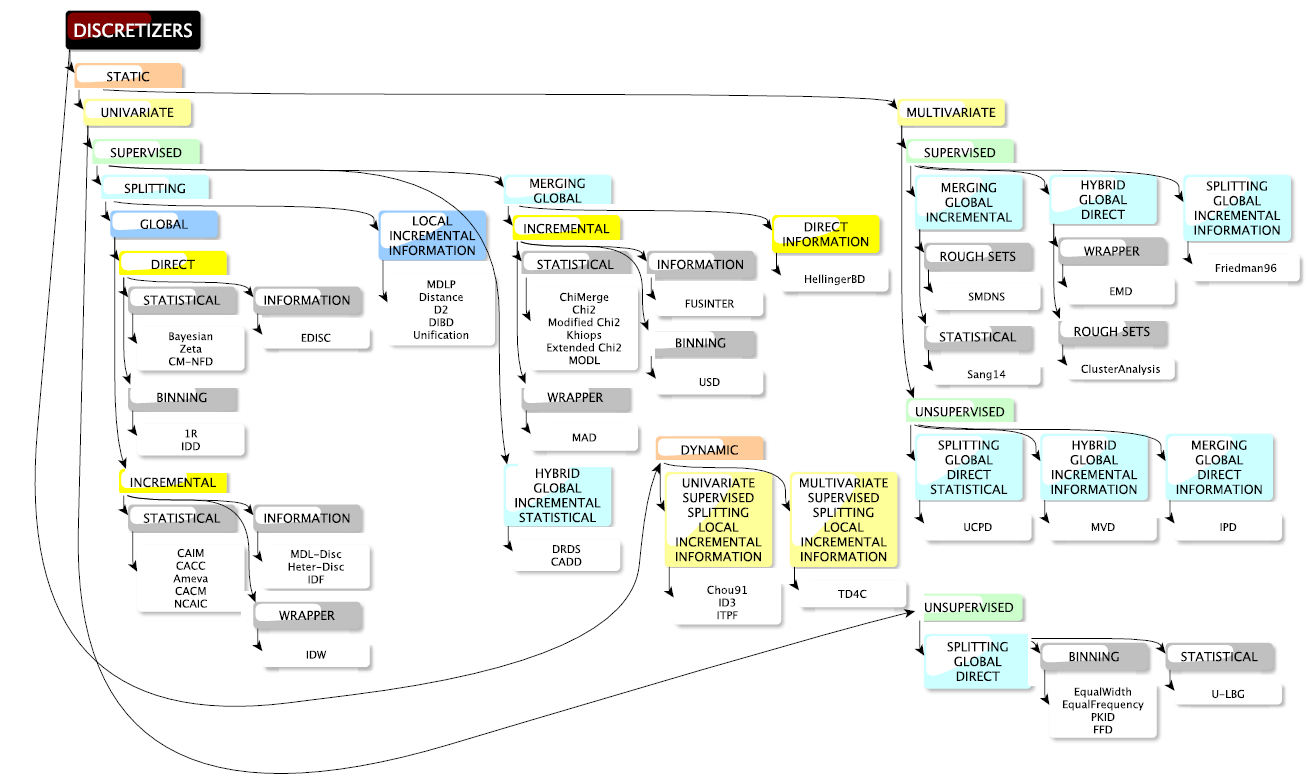
\includegraphics[scale=0.3]{figures/taxonomy.PNG}
\end{center}
\vspace*{-0.2cm}
These approaches\footcite{wrapper2} maximize an ``intermediary'' criterion, \textit{e.g.}:
\vspace*{-0.1cm}
\begin{minipage}[c]{0.15\linewidth}
\begin{animateinline}[poster=first,loop]{2}%
{\color{orange}{\bf CACF}}%
\newframe \end{animateinline}
\end{minipage}
\begin{minipage}[c]{0.8\linewidth}
\[ \hat{\q}_j^{\chi^2} = \argmax_{\q_j} \chi^2(\q_j(\mathbf{x}_\text{f}), \mathbf{y}_\text{f}) \stackrel{?}{\approx} \q^\star_j, \]
\end{minipage}
\vspace*{-0.1cm}
and we {\bf hope} that it's aligned with our original goal s.t.:
%\vspace*{-0.1cm}

\begin{minipage}[c]{0.15\linewidth}
\begin{animateinline}[poster=first,loop]{2}%
{\color{orange}{\bf CACF}}%
\newframe \end{animateinline}
\end{minipage}
\begin{minipage}[c]{0.8\linewidth}
\[ \hat{\bm{\theta}}^{\chi^2} = \argmax_{\bm{\theta}} \ell(\bm{\theta} ; \mathbf{y}_\text{f}, {\hat{\q}^{\chi^2}}(\mathbf{x}_\text{f})) \stackrel{?}{\approx} \bm{\theta}^\star. \]
\end{minipage}
\vspace*{0.1cm}

\end{frame}






\subsection{research contribution}
\begin{frame}
\frametitle{\secname: \subsecname}

%%%%%%%%%
\note{
On a décidé de prendre une toute autre proche, toujours dans l'espoir d'apporter une formalisation et une résolution plus directe au problème original de sélection de modèle.

\bigskip

La première difficulté réside dans le fait que la quantification est un problème discret qu'on peut donc difficilement optimiser directement sans tester toutes les combinaisons

\bigskip

C'est pourquoi on relaxe le problème en paramétrant la quantification q par alpha, c'est-à-dire à utiliser des fonctions "douces", continues et dérivables de type softmax.

\bigskip

On peut l'interpréter comme la possibilité d'être dans plusieurs intervalles simultanément à des proportions différentes, ce qu'on peut simplement illustrer...


}
%%%%%%%%%

\textcolor{green}{``Soft'' approximation}:

\begin{equation*}
    \q_{\ag_j}(\cdot)=\left(q_{\ag_{j,h}}(\cdot)\right)_{h=1}^{m_j} \text{ with } \begin{cases} \sum_{h=1}^{m_j}q_{\ag_{j,h}}(\cdot)=1, \\ 0 \leq q_{\ag_{j,h}}(\cdot) \leq 1, \end{cases}
\end{equation*}

\uncover<2->{

\textbf{For continuous features}, we set for $\bm{\alpha}_{j,h} = (\alpha^0_{j,h},\alpha^1_{j,h}) \in \mathbb{R}^2$
\[\s_{\ag_{j,h}}(\cdot) = \frac{\exp(\alpha^0_{j,h} + \alpha^1_{j,h}  \cdot)}{\sum_{g=1}^{m_j} \exp(\alpha^0_{j,g} + \alpha^1_{j,g}  \cdot)}.\]
}
\uncover<3->{

\textbf{For categorical features}, we set for $\bm{\alpha}_{j,h}=\left(\alpha_{j,h}(1),\ldots, \alpha_{j,h}(l_j)\right) \in \mathbb{R}^{l_j}$
\[\s_{\ag_{j,h}}(\cdot) = \frac{\exp\left(\alpha_{j,h}(\cdot)\right)}{\sum_{g=1}^{m_j} \exp\left(\alpha_{j,g}(\cdot)\right)}.\]
}

\end{frame}





\subsection{MAP estimation}
\begin{frame}
\frametitle{\secname : \subsecname}


%%%%%%%%%%
\note{

... avec 3 softmax cherchant à estimer 3 vraies quantifications dont les points de coupure sont en orange

\bigskip

Dans cet exemple, on a par exemple une proba de 80 pourcent d'être dans le premier intervalle, de 15 pourcent dans le second et de 5 pourcent dans le dernier.

\bigskip

A supposer qu'on puisse estimer les paramètres alpha chapeau donnés ici, on peut même "forcer" la quantification "douce" q alpha à redevenir une vraie quantification, c'est-à-dire des créneaux, en réalisant une estimation du maximum a posteriori : là où la première modalité est "majoritaire" donc > 33 pourcent dans cet exemple, on considère que c'est le premier intervalle. Ca nous permet de retrouver les points de coupure orange.

}
%%%%%%%%%%


\vspace*{-0.4cm}

\[ \hat{\s}_{j,h}(x_j) = 1 \text{ if } h = \argmax_{1 \leq h' \leq m_j} \s_{\hat{\ag}_{j,h'}}, 0 \text{ otherwise\footcite{chamroukhi2009regression}$^{,}$\footcite{same2011model}.} \]

\begin{tikzpicture}[scale=0.9]
\begin{axis}[
  no markers, domain=-1.5:2, samples=100,
  axis lines*=left,
  every axis y label/.style={at=(current axis.left of origin), anchor=north west},
  height=3cm, width=11cm,
  xtick=\empty, ytick=\empty,
  enlargelimits=false, clip=false,
  x label style={at={(axis description cs:0.5,0.3)},anchor=north},
  y label style={at={(axis description cs:-0.1,.5)},rotate=90,anchor=south},
  xlabel={$x_j$},
  ylabel={$\s_{\hat{\ag}_{j,1}}(x_j)$}
  ]
   
   \mode<beamer>{ 
  \addplot [very thick,white] {gauss(-1.8,0.6)};
  }
  \mode<handout>{
  \addplot [very thick,black] {gauss(-1.8,0.6)};
  }
\addplot+[mark=none,ultra thick,orange] coordinates {(-0.7,0) (-0.7,0.6)};
\addplot+[mark=none,ultra thick,orange] coordinates {(1,0) (1,0.6)};
\node at (axis cs:-1.1,0.4) {$\hat{\s}_{j,1}(x_j)=1$};
\node at (axis cs:0,0.4) {$\hat{\s}_{j,1}(x_j)=0$};
\node at (axis cs:1.5,0.4) {$\hat{\s}_{j,1}(x_j)=0$};
\node at (axis cs:-0.7,-0.15) {$\hat{c}_{j,1}$};
\node at (axis cs:1,-0.15) {$\hat{c}_{j,2}$};

\end{axis}
\end{tikzpicture}
\vspace*{-0.3cm}
\begin{tikzpicture}[scale=0.9]
\begin{axis}[
  no markers, domain=-1.5:2, samples=100,
  axis lines*=left,
  every axis y label/.style={at=(current axis.left of origin), anchor=north west},
  height=3cm, width=11cm,
  xtick=\empty, ytick=\empty,
  enlargelimits=false, clip=false,
  x label style={at={(axis description cs:0.5,0.3)},anchor=north},
  y label style={at={(axis description cs:-0.1,.5)},rotate=90,anchor=south},
  xlabel={$x_j$},
  ylabel={$\s_{\hat{\ag}_{j,2}}(x_j)$}
  ]
   \mode<beamer>{
  \addplot [very thick,white] {gauss(0,0.6)};
  }
  \mode<handout>{
  \addplot [very thick,black] {gauss(0,0.6)};
  }
\addplot+[mark=none, ultra thick,orange] coordinates {(-0.7,0) (-0.7,0.6)};
\addplot+[mark=none, ultra thick,orange] coordinates {(1,0) (1,0.6)};
\node at (axis cs:-1.1,0.4) {$\hat{\s}_{j,2}(x_j)=0$};
\node at (axis cs:0,0.4) {$\hat{\s}_{j,2}(x_j)=1$};
\node at (axis cs:1.5,0.4) {$\hat{\s}_{j,2}(x_j)=0$};
\node at (axis cs:-0.7,-0.15) {$\hat{c}_{j,1}$};
\node at (axis cs:1,-0.15) {$\hat{c}_{j,2}$};

\end{axis}

\end{tikzpicture}
\vspace*{-0.3cm}
\begin{tikzpicture}[scale=0.9]
\begin{axis}[
  no markers, domain=-1.5:2, samples=100,
  axis lines*=left,
  every axis y label/.style={at=(current axis.left of origin), anchor=north west},
  height=3cm, width=11cm,
  xtick=\empty, ytick=\empty,
  enlargelimits=false, clip=false,
  x label style={at={(axis description cs:0.5,0.3)},anchor=north},
  y label style={at={(axis description cs:-0.1,.5)},rotate=90,anchor=south},
  xlabel={$x_j$},
  ylabel={$\s_{\hat{\ag}_{j,3}}(x_j)$}
  ]
    
   \mode<beamer>{
  \addplot [very thick,white] {gauss(2,0.6)};
  }
  \mode<handout>{
  \addplot [very thick,black] {gauss(2,0.6)};
  }

\addplot+[mark=none, ultra thick,orange] coordinates {(-0.7,0) (-0.7,0.6)};
\addplot+[mark=none, ultra thick,orange] coordinates {(1,0) (1,0.6)};

\node at (axis cs:-1.1,0.4) {$\hat{\s}_{j,3}(x_j)=0$};
\node at (axis cs:0,0.4) {$\hat{\s}_{j,3}(x_j)=0$};
\node at (axis cs:1.5,0.4) {$\hat{\s}_{j,3}(x_j)=1$};
\node at (axis cs:-0.7,-0.15) {$\hat{c}_{j,1}$};
\node at (axis cs:1,-0.15) {$\hat{c}_{j,2}$};

\end{axis}
\end{tikzpicture}

\hspace*{0.5cm}
\end{frame}





\subsection{neural networks}

\begin{frame}
\frametitle{\secname: \subsecname}


%%%%%%%%%%
\note{
Pour estimer de bons paramètres alpha, on se plonge encore une fois dans le cadre de la vraisemblance...

\bigskip

... qu'on aimerait maximiser en $\theta$ et $\alpha$ ce qui nous conduirait, d'après les propriétés du maximum de vraisemblance, à retrouver au moins asymptotiquement le vrai mécanisme de génération des données, c-à-d la vraie quantification

\bigskip

sauf que on ne peut pas maximiser cette vraisemblance directement, donc on utilise également une heuristique : la descente de gradient.

}
%%%%%%%%%%



We wish to maximize the following likelihood:
\[ (\hat{\bm{\theta}}, \hat{\bm{\alpha}}) = \argmax_{\bm{\theta}, \bm{\alpha}} \ell(\bm{\theta}, \bm{\alpha} ; \bm{\mathbf{x}}_\f, \bm{\mathbf{y}}_\f) = \argmax_{\bm{\theta}, \bm{\alpha}} \sum_{i=1}^n \ln p_{\bm{\theta}}(y_i | \q_{\alpha}(\bm{x}_i)). \]

\medskip

``$\bm{\alpha}^\star = \lim_{n \to \infty} \hat{\bm{\alpha}}$'' should be such that \textcolor{green}{$\q_{\bm{\alpha}^\star} = \q^\star$}.

\medskip

\uncover<2->{
Problem: $\hat{\bm{\alpha}}$ has to \textcolor{green}{diverge}, the MLE is at the border of the parameter space which could hinder its properties.
}

\medskip

\uncover<3->{
Anyway, or more generally if there is no true quantization $\q^\star$, 

$\hat{\q}$ is used instead as a \textcolor{green}{quantization candidate}.
}

\medskip

\uncover<4->{
{\bf Problem:} $\ell(\bm{\theta}, \bm{\alpha} ; \bm{\mathbf{x}}_\f, \bm{\mathbf{y}}_\f)$ cannot be directly maximized.
}

\medskip

\uncover<4->{
{\bf Solution:} Resort to (stochastic) gradient descent which \textcolor{green}{each step $(s)$ will yield} $\hat{\bm{\alpha}}^{(s)}$ and \textcolor{green}{quantization candidate $\hat{\q}^{(s)}$}.
}

\end{frame}






\begin{frame}
\frametitle{\secname: \subsecname}

%%%%%%%%%%
\note{C'est là que la paramétrisation sous la forme de softmax prend son sens puisqu'on peut écrire le modèle comme un réseau de neurones très simple.

\bigskip

On peut donc s'appuyer sur les librairies logicielles standards de réseaux de neurones, qui marchent bien et très vite.

\bigskip

Ces réseaux de neurones peu profonds sont moins sensibles à tous les hyper-paramètres, qui ont néanmoins été optimisés pour les expériences. 

Par ailleurs, c'est juste un moyen de se promener dans l'espace sans qu'il y ait nécessairement convergence de l'algorithme.
}
%%%%%%%%%%


Very simple neural network.

Very fast implementations available, \textit{e.g.}\ TensorFlow.

\textbf{No guarantee} of global optimum (but works well in practice).

\def\layersep{2.5cm}

\centering
\begin{tikzpicture}[shorten >=1pt,->,draw=black!50, node distance=\layersep]
    \tikzstyle{every pin edge}=[<-,shorten <=1pt]
    \tikzstyle{neuron}=[circle,fill=black!25,minimum size=17pt,inner sep=0pt]
    \tikzstyle{input neuron}=[neuron, fill=green!50];
    \tikzstyle{output neuron}=[neuron, fill=red!50];
    \tikzstyle{hidden neuron}=[neuron, fill=blue!50];
    \tikzstyle{annot} = [text width=4em, text centered]
    \tikzstyle{annotrectangle} = [text width=8em, text centered]


        \node[input neuron, pin=left:Continuous input \#1] (I-1) at (0,-1) {};
        
        \node[input neuron, pin=left:Level \#1] (I-2) at (0,-2) {};
        \node[input neuron, pin=left:Level \#2] (I-3) at (0,-3) {};
        \node[input neuron, pin=left:Level \#3] (I-4) at (0,-4) {};

    % Draw the hidden layer nodes
    \foreach \name / \y in {1,...,2}
        \path[yshift=0.5cm]
            node[hidden neuron] (H-\name) at (\layersep,-\y cm) {Soft};

    \foreach \name / \y in {3,...,4}
        \path[yshift=0.5cm]
            node[hidden neuron] (H-\name) at (\layersep,-\y cm) {Soft};

    % Draw the output layer node
    \node[output neuron,pin={[pin edge={->}]right:Output}, right of=H-2] (O) {$\sigma$};

    % Connect every node in the input layer with every node in the
    % hidden layer.
%    \foreach \source in {1,...,4}
        \foreach \dest in {1,2}
            \path (I-1) edge (H-\dest);

        \foreach \dest in {3,4}
            \path (I-2) edge (H-\dest);
        \foreach \dest in {3,4}
            \path (I-3) edge (H-\dest);
        \foreach \dest in {3,4}
            \path (I-4) edge (H-\dest);

        % \foreach \dest in {5,6}
        %     \path (I-3) edge (H-\dest);

    % Connect every node in the hidden layer with the output layer
    \foreach \source in {1,...,4}
        \path (H-\source) edge (O);

    % Annotate the layers
    \node[annot,above of=H-1, node distance=1cm] (hl) {Hidden layer};
    \node[annot,left of=hl] {Input layer};
    \node[annot,right of=hl] {Output layer};
    
    
    \draw [orange] (2,0) rectangle (3,-1.9);
    \draw [orange] (-0.5,-0.5) rectangle (0.5,-4.5);
    
    \node[annotrectangle,right of=H-1, node distance=2.5cm] {\textcolor{green}{Softmax outputs are $\q_{{\ag}_j}(x_j)$}.}; 
    

\end{tikzpicture}

\textcolor{green}{Multivariate quantization!}

\end{frame}





\newlength\figureheight
\newlength\figurewidth
\setlength\figureheight{7cm}
\setlength\figurewidth{12cm}
 
\begin{frame}
\frametitle{\secname: \subsecname}

%%%%%%%%%%
\note{On peut donc regarder les estimations successives des paramètres alpha et les quantifications "douces" qui en résultent quand on simule une vraie discrétisation à 3 modalités avec 5 softmax (donc 5 modalités au maximum).

\bigskip

Les vrais points de coupure sont en pointillés (1/3 et 2/3).

\bigskip

Au départ, seuls 2 softmax s'activent et au fur et à mesure des itérations, on a bien 3 softmax qui ressemblent à des créneaux.
}
%%%%%%%%%%


\mode<beamer>{
\begin{figure}
\hspace*{-1cm}
\begin{animateinline}[poster=first, controls, buttonfg=white]{3}
\multiframe{200}{i=1+1}{\input{CODE_FIGURES/GLMDISC_NN/feature_0_iteration_\i.tex}}%
\end{animateinline}
\end{figure}
}

\mode<handout>{
% This file was created by matplotlib2tikz v0.6.18.
\begin{tikzpicture}

\definecolor{color0}{rgb}{0,0.75,0.75}
\definecolor{color1}{rgb}{0.75,0,0.75}
\definecolor{color2}{rgb}{0.75,0.75,0}

\begin{axis}[
height=\figureheight,
legend cell align={left},
legend entries={{${q}_{\bm{\alpha}_{0,0}}$},{${q}_{\bm{\alpha}_{0,1}}$},{${q}_{\bm{\alpha}_{0,2}}$},{${q}_{\bm{\alpha}_{0,3}}$},{${q}_{\bm{\alpha}_{0,4}}$},{$c_{0,1}$},{$c_{0,2}$},{$\hat{c}_{0,2}$},{$\hat{c}_{0,3}$}},
legend style={at={(0.91,0.5)}, anchor=east, draw=white!80.0!black},
tick align=outside,
tick pos=left,
title={Continuous feature 0 at iteration 100},
width=\figurewidth,
x grid style={white!69.01960784313725!black},
xlabel={$x_1$},
xmin=0, xmax=1,
y grid style={white!69.01960784313725!black},
ylabel={${q}_{\bm{\alpha}_{0,h}}$},
ymin=0, ymax=1
]
\addlegendimage{no markers, red}
\addlegendimage{no markers, color0}
\addlegendimage{no markers, color1}
\addlegendimage{no markers, color2}
\addlegendimage{no markers, black}
\addlegendimage{no markers, green!50.0!black}
\addlegendimage{no markers, blue}
\addlegendimage{no markers, green!50.0!black}
\addlegendimage{no markers, blue}
\addplot [thick, red]
table [row sep=\\]{%
0.0011059794751318	0.999458491802216 \\
0.00144600828615515	0.999453961849213 \\
0.00151620394328711	0.999453127384186 \\
0.00161381928831428	0.99945205450058 \\
0.00193644961641948	0.999447762966156 \\
0.0024363370221504	0.99944144487381 \\
0.00384167794354173	0.999423027038574 \\
0.00421063900202368	0.999417901039124 \\
0.00632372037002726	0.999388813972473 \\
0.00947686783375368	0.999342501163483 \\
0.0099356428556221	0.999335467815399 \\
0.0101317191976503	0.99933248758316 \\
0.0102519961026396	0.999330639839172 \\
0.0116572936797861	0.999308466911316 \\
0.0122763055741271	0.999298453330994 \\
0.0128807282915644	0.999288558959961 \\
0.0131006826676461	0.999285042285919 \\
0.0132105085232722	0.999283134937286 \\
0.0150477352877949	0.999252021312714 \\
0.0151511241047927	0.999250113964081 \\
0.0168553495563415	0.999220132827759 \\
0.0191895991753259	0.999176800251007 \\
0.0192724193499449	0.999175131320953 \\
0.0202131188025382	0.999157190322876 \\
0.0251886934986562	0.999054133892059 \\
0.0255409812646521	0.999046385288239 \\
0.0256196546755231	0.999044716358185 \\
0.0263800727822662	0.999027729034424 \\
0.026825697968402	0.999017596244812 \\
0.0272388337061176	0.999008357524872 \\
0.0276781997826389	0.99899810552597 \\
0.0277969734855988	0.998995363712311 \\
0.027888291941232	0.998993098735809 \\
0.032801074197002	0.998872101306915 \\
0.0337126623182875	0.998847961425781 \\
0.0349109578825388	0.998815655708313 \\
0.0367757145561887	0.99876344203949 \\
0.0368887253476963	0.998760223388672 \\
0.0376301111814882	0.998738706111908 \\
0.0383020767002249	0.998718976974487 \\
0.0385765124363792	0.998710751533508 \\
0.0386281055032889	0.998709201812744 \\
0.0397134557815922	0.998676478862762 \\
0.0400530872540832	0.998665928840637 \\
0.0408224228009035	0.998642027378082 \\
0.042416614098386	0.998591005802155 \\
0.042542997860721	0.998586893081665 \\
0.0425634328976269	0.998586297035217 \\
0.0426938593122377	0.998582005500793 \\
0.0436353215690566	0.998550713062286 \\
0.0476491609572692	0.998409748077393 \\
0.0476764809468383	0.998408854007721 \\
0.0480632979275277	0.998394429683685 \\
0.0489335324060199	0.998361885547638 \\
0.0494953541501341	0.998340368270874 \\
0.0498656975684827	0.998326122760773 \\
0.0507299142819697	0.99829238653183 \\
0.0520149216066462	0.998240947723389 \\
0.053491737186121	0.998179793357849 \\
0.0545456118282759	0.998134851455688 \\
0.0549368100196436	0.998117923736572 \\
0.0549667939602374	0.998116612434387 \\
0.0555159955251522	0.998092472553253 \\
0.0574839546417889	0.998003900051117 \\
0.0576927502423773	0.997994184494019 \\
0.0580609228746025	0.997976958751678 \\
0.0610070220733733	0.997834384441376 \\
0.0613718310828713	0.99781608581543 \\
0.0624819644863142	0.997759342193604 \\
0.0632024977130776	0.99772173166275 \\
0.0641707318537266	0.997670114040375 \\
0.064803290117067	0.997635960578918 \\
0.0661546388560771	0.997560858726501 \\
0.0675945492445934	0.997478306293488 \\
0.0701208744758773	0.997326850891113 \\
0.0704495440664726	0.997306346893311 \\
0.0707913481046274	0.997285127639771 \\
0.0709503961374458	0.997275054454803 \\
0.0723079949898875	0.99718827009201 \\
0.0729582139062805	0.997145712375641 \\
0.0736427592129116	0.997100174427032 \\
0.0738431652021745	0.997086822986603 \\
0.074094042941424	0.997069835662842 \\
0.0741988699821797	0.997062742710114 \\
0.0745344402647278	0.997039973735809 \\
0.0761651718345726	0.996926248073578 \\
0.0762565104011357	0.996919870376587 \\
0.0764247618188199	0.996907889842987 \\
0.0780473992355428	0.996789753437042 \\
0.0784939963588281	0.996756494045258 \\
0.0787288834363844	0.996738970279694 \\
0.0796528614743472	0.996668636798859 \\
0.0821291956626848	0.996472537517548 \\
0.0836539892117674	0.996346414089203 \\
0.0837976822096664	0.996334075927734 \\
0.0840863722935196	0.996309459209442 \\
0.0847664004367794	0.996251285076141 \\
0.0848642352310873	0.996242880821228 \\
0.0852150851090396	0.996212244033813 \\
0.085891869345856	0.996152579784393 \\
0.087068315817913	0.996046602725983 \\
0.0885849846877879	0.995905876159668 \\
0.0903431131516136	0.995736479759216 \\
0.0909278592293694	0.995678722858429 \\
0.0914296081009306	0.995628476142883 \\
0.0922298300096035	0.995546936988831 \\
0.0926517333242025	0.995503485202789 \\
0.0930086769471365	0.995466232299805 \\
0.0936368650628759	0.995400130748749 \\
0.0939832817677504	0.995363235473633 \\
0.0963578674192209	0.995102286338806 \\
0.0969604240071604	0.995033979415894 \\
0.0974174263218397	0.994981229305267 \\
0.0997464409700664	0.99470454454422 \\
0.100249930959155	0.994642734527588 \\
0.100820744388044	0.99457198381424 \\
0.101229398304142	0.994520545005798 \\
0.102271393895604	0.994387447834015 \\
0.102325882258744	0.994380295276642 \\
0.103474916599901	0.994229674339294 \\
0.104369461810087	0.994109749794006 \\
0.104849386693897	0.994044125080109 \\
0.105274572558957	0.993985593318939 \\
0.105437385176067	0.993962943553925 \\
0.105718642159513	0.993923723697662 \\
0.106451679001465	0.993820369243622 \\
0.106754108203929	0.993777275085449 \\
0.106889477031479	0.993757724761963 \\
0.108308586301563	0.993550419807434 \\
0.108355506097126	0.99354350566864 \\
0.110864090628752	0.993159890174866 \\
0.112062699234041	0.992968618869781 \\
0.112686863552251	0.992867112159729 \\
0.113787419472266	0.992684185504913 \\
0.114114908535732	0.992628931999207 \\
0.114926076298882	0.992490112781525 \\
0.115710925433917	0.99235337972641 \\
0.116193807044869	0.992268145084381 \\
0.116352662276253	0.992239713668823 \\
0.116979956596317	0.992127299308777 \\
0.117247317403657	0.992078721523285 \\
0.118793828877862	0.99179220199585 \\
0.119352906137166	0.991686046123505 \\
0.120388240876593	0.991486012935638 \\
0.122357154089364	0.991092264652252 \\
0.125712799722249	0.990379214286804 \\
0.126988316690772	0.990093529224396 \\
0.130289689058528	0.989314675331116 \\
0.130830575131366	0.989181578159332 \\
0.13178708265069	0.98894190788269 \\
0.132217070962463	0.988832354545593 \\
0.132641072460891	0.988723397254944 \\
0.133694684584262	0.988447964191437 \\
0.135586813424106	0.987936794757843 \\
0.136970534315695	0.98754870891571 \\
0.137167897059254	0.987492322921753 \\
0.13731957841644	0.987448930740356 \\
0.138770949832641	0.987025320529938 \\
0.141579671494468	0.986165285110474 \\
0.142337772861435	0.985923647880554 \\
0.142852169410084	0.985757350921631 \\
0.14313843453823	0.985664010047913 \\
0.143709892765619	0.985475838184357 \\
0.143996587198751	0.985380351543427 \\
0.144338718134467	0.985265791416168 \\
0.145474509131844	0.984878957271576 \\
0.146058924442183	0.984675943851471 \\
0.147496370200373	0.98416543006897 \\
0.147934500473159	0.984006583690643 \\
0.148464696403164	0.983812153339386 \\
0.149007159183894	0.98361074924469 \\
0.151290695331351	0.982735872268677 \\
0.153507740604538	0.981842756271362 \\
0.153927498261582	0.981668651103973 \\
0.153953160827713	0.981657862663269 \\
0.154179436777791	0.981563448905945 \\
0.155107736993068	0.981170117855072 \\
0.15519005879533	0.981135010719299 \\
0.155418402417591	0.98103666305542 \\
0.156078407887877	0.980750262737274 \\
0.158100170599977	0.979845941066742 \\
0.158283533549941	0.979761958122253 \\
0.158599777942073	0.979616165161133 \\
0.159258263288539	0.979309320449829 \\
0.159678910282026	0.979111015796661 \\
0.162540881855109	0.977711379528046 \\
0.164077384668961	0.976922392845154 \\
0.164957348092599	0.976458311080933 \\
0.165030574098427	0.97641932964325 \\
0.165280388241905	0.976285696029663 \\
0.167273692684132	0.975193083286285 \\
0.168043854724866	0.974757850170135 \\
0.168088628486329	0.974732220172882 \\
0.168662857989897	0.974402546882629 \\
0.169151147716595	0.974118947982788 \\
0.169673214248392	0.973812282085419 \\
0.170135609058708	0.973537802696228 \\
0.171767974673073	0.972545981407166 \\
0.1728518498484	0.971867799758911 \\
0.172984599941167	0.971783459186554 \\
0.176370551959836	0.969551742076874 \\
0.176588273575192	0.969402492046356 \\
0.176656553576852	0.969355404376984 \\
0.17794804219768	0.968454301357269 \\
0.178429717033185	0.968111872673035 \\
0.179458814233081	0.96736752986908 \\
0.180595104426831	0.966526567935944 \\
0.18064479669491	0.966489195823669 \\
0.182294707450728	0.965229094028473 \\
0.182819109355123	0.964819192886353 \\
0.189141614514094	0.959495484828949 \\
0.190723527970293	0.958047330379486 \\
0.192508826701743	0.956353306770325 \\
0.200712508340217	0.947697281837463 \\
0.202130410523186	0.94604504108429 \\
0.202705868873484	0.945360779762268 \\
0.202975660615516	0.945037126541138 \\
0.2033001668374	0.944645285606384 \\
0.204138047670012	0.943621695041656 \\
0.204584283026216	0.943069279193878 \\
0.205975712225296	0.941313982009888 \\
0.208693969096644	0.937737762928009 \\
0.209097012308874	0.937190473079681 \\
0.210129299396579	0.935768187046051 \\
0.210470524326312	0.935291528701782 \\
0.210726758187617	0.934931337833405 \\
0.210879765452585	0.934715509414673 \\
0.213404555935633	0.931054770946503 \\
0.214779680955682	0.928981900215149 \\
0.215976334819965	0.927131414413452 \\
0.21605980843853	0.927000761032104 \\
0.21626681121775	0.92667555809021 \\
0.217333435243771	0.924979150295258 \\
0.217860184045886	0.92412805557251 \\
0.218810300034316	0.922570407390594 \\
0.219036830922259	0.922194838523865 \\
0.219186045259484	0.92194652557373 \\
0.219509161852637	0.921406388282776 \\
0.219517283100912	0.921392619609833 \\
0.220007941128277	0.920565485954285 \\
0.221124031401732	0.918654501438141 \\
0.221655686766872	0.917729377746582 \\
0.222787328400317	0.915728688240051 \\
0.222812240344664	0.915684163570404 \\
0.224413114839207	0.912776827812195 \\
0.225712117798195	0.91035133600235 \\
0.226064824403414	0.909682393074036 \\
0.22778297811216	0.906358957290649 \\
0.227786137279108	0.906352698802948 \\
0.228255816092263	0.905425429344177 \\
0.22886379454373	0.904212653636932 \\
0.229286896531361	0.903360366821289 \\
0.231570483736477	0.89864319562912 \\
0.232839821990075	0.895933747291565 \\
0.234699792231533	0.891847908496857 \\
0.236598748956898	0.887531638145447 \\
0.236914864918852	0.886798679828644 \\
0.238193170258512	0.883792281150818 \\
0.238267801131912	0.883614659309387 \\
0.241280255564163	0.87624454498291 \\
0.241532477911657	0.875609517097473 \\
0.242724887440966	0.872570216655731 \\
0.243487528482621	0.870592892169952 \\
0.243851755033328	0.86963963508606 \\
0.243931127736832	0.869431018829346 \\
0.245492487219521	0.865270256996155 \\
0.245961870318215	0.863997936248779 \\
0.247220233087027	0.860536515712738 \\
0.248029547774932	0.858271539211273 \\
0.248195183805212	0.857804298400879 \\
0.252597476547261	0.844907104969025 \\
0.254049623190913	0.840448141098022 \\
0.254469169693275	0.839141070842743 \\
0.254777550536903	0.838174521923065 \\
0.254877558399671	0.83786016702652 \\
0.257253649731868	0.830243706703186 \\
0.257671137054733	0.828876376152039 \\
0.26187840669548	0.814608097076416 \\
0.264182169008257	0.806413590908051 \\
0.265462287195374	0.801742911338806 \\
0.267638564660905	0.793608427047729 \\
0.268216851612881	0.791405916213989 \\
0.269980014659659	0.784583747386932 \\
0.270837940398052	0.78120619058609 \\
0.271133018969332	0.780035793781281 \\
0.271522794293612	0.778482913970947 \\
0.272730212426688	0.773622691631317 \\
0.27325151773824	0.771501064300537 \\
0.273458501731612	0.770654559135437 \\
0.275787496734588	0.76098108291626 \\
0.275790346826632	0.760969281196594 \\
0.275963502468307	0.760238528251648 \\
0.276441724078765	0.758214175701141 \\
0.277788622824976	0.752448797225952 \\
0.278249554181787	0.750454545021057 \\
0.278902433397602	0.747611939907074 \\
0.280228184178203	0.741774141788483 \\
0.282170737525181	0.733062386512756 \\
0.284775883532131	0.721089720726013 \\
0.285319633849948	0.718549907207489 \\
0.285945143849347	0.715610265731812 \\
0.287293498153222	0.709211945533752 \\
0.288098109983407	0.705353438854218 \\
0.288474372887691	0.703538954257965 \\
0.288733693686359	0.702284514904022 \\
0.291563977198166	0.688398838043213 \\
0.293976605993451	0.676287174224854 \\
0.294014528290392	0.676095366477966 \\
0.294718175832172	0.672515571117401 \\
0.294831463459233	0.671937704086304 \\
0.294887681144015	0.671650469303131 \\
0.299064488228799	0.649971663951874 \\
0.299223468133874	0.649133265018463 \\
0.299853491506122	0.645802199840546 \\
0.301624334890634	0.636365175247192 \\
0.302100714632492	0.633807897567749 \\
0.302855829384862	0.62973940372467 \\
0.303468685820656	0.626423060894012 \\
0.304335545384868	0.621712744235992 \\
0.305081848845274	0.61763870716095 \\
0.305263786725066	0.616643071174622 \\
0.305511643802704	0.615285038948059 \\
0.30635774546767	0.610635459423065 \\
0.307937429467832	0.601901531219482 \\
0.308578187230734	0.598340213298798 \\
0.313991998160918	0.567867815494537 \\
0.315973848719028	0.556569874286652 \\
0.317413649622303	0.548324108123779 \\
0.319657848506035	0.535420715808868 \\
0.319781920771261	0.534706115722656 \\
0.320496004308145	0.530588924884796 \\
0.320601310305949	0.529980838298798 \\
0.322246867517597	0.520476818084717 \\
0.323306124649751	0.514350593090057 \\
0.323664358184811	0.512277781963348 \\
0.323805398711091	0.511461675167084 \\
0.324816846999054	0.505606234073639 \\
0.325263683488062	0.503019154071808 \\
0.327533460856979	0.489877432584763 \\
0.328385869951453	0.48494428396225 \\
0.329844054701458	0.476513266563416 \\
0.33074904970515	0.47128689289093 \\
0.332974695502457	0.458463728427887 \\
0.333600133199531	0.454869210720062 \\
0.336001356191777	0.441115915775299 \\
0.338057278352338	0.42941090464592 \\
0.33940563378102	0.421776324510574 \\
0.339522610836627	0.421115398406982 \\
0.341295751839904	0.41113755106926 \\
0.343025583329651	0.401472419500351 \\
0.344156227439929	0.395196288824081 \\
0.344485478041551	0.393375039100647 \\
0.346631556569637	0.3815778195858 \\
0.348247004908186	0.372788101434708 \\
0.348257869791207	0.372728854417801 \\
0.350134953366802	0.362621426582336 \\
0.352271571140202	0.351262927055359 \\
0.352403536611892	0.350566059350967 \\
0.356607161458692	0.328733652830124 \\
0.357473355861859	0.324321895837784 \\
0.359032837138255	0.31645679473877 \\
0.360085447455855	0.311206847429276 \\
0.360587038984981	0.308721750974655 \\
0.3618814720936	0.3023601770401 \\
0.362541325151431	0.29914590716362 \\
0.363971114014582	0.292249143123627 \\
0.36446377318254	0.289894372224808 \\
0.364734654416428	0.288604557514191 \\
0.364782079325344	0.288379013538361 \\
0.36626622804169	0.281376153230667 \\
0.36745676602671	0.275833666324615 \\
0.367555756327517	0.275376051664352 \\
0.367766921022286	0.274401098489761 \\
0.368015883464081	0.273254245519638 \\
0.368183587302196	0.272483736276627 \\
0.368646745255496	0.270362168550491 \\
0.368824340831231	0.269551396369934 \\
0.36908666014638	0.268356829881668 \\
0.370227788452905	0.263199061155319 \\
0.371079364739364	0.259391784667969 \\
0.371457393668236	0.257713198661804 \\
0.372521553247257	0.253026008605957 \\
0.372816229090882	0.251738220453262 \\
0.373696444358129	0.247917339205742 \\
0.375236418301489	0.241326555609703 \\
0.375355278624935	0.240822806954384 \\
0.375592850161798	0.239818170666695 \\
0.375621310337888	0.239697962999344 \\
0.37623340048021	0.237123653292656 \\
0.376649481158299	0.235384926199913 \\
0.37682934901581	0.234635785222054 \\
0.377022374188538	0.233833596110344 \\
0.378777395062222	0.226630032062531 \\
0.379219181502585	0.224841311573982 \\
0.380639994297166	0.219157502055168 \\
0.381635433931239	0.215237319469452 \\
0.382416367624347	0.212197810411453 \\
0.383276747323035	0.208885386586189 \\
0.383441774868681	0.208254262804985 \\
0.384589480637987	0.203904837369919 \\
0.38762147240542	0.192741647362709 \\
0.387652450706726	0.192629858851433 \\
0.38818745089578	0.190709978342056 \\
0.388531576179462	0.189482718706131 \\
0.391108514236782	0.180485114455223 \\
0.391741157295481	0.17832787334919 \\
0.396723908263121	0.162039205431938 \\
0.39803082540264	0.157970547676086 \\
0.398171926406937	0.157536283135414 \\
0.398666017137866	0.156023189425468 \\
0.398819673578751	0.155555129051208 \\
0.4012576168302	0.148280769586563 \\
0.402752737045505	0.143959984183311 \\
0.403290070599278	0.142433032393456 \\
0.404563584871068	0.138867616653442 \\
0.406532702382757	0.133502542972565 \\
0.406578018270242	0.13338129222393 \\
0.413273296435021	0.116451136767864 \\
0.413592377461711	0.115692868828773 \\
0.41401191876112	0.114702187478542 \\
0.414776267969876	0.112916633486748 \\
0.414785799829368	0.112894527614117 \\
0.415238430177184	0.111848704516888 \\
0.416465974154779	0.109055124223232 \\
0.416689013292801	0.10855408012867 \\
0.418297500020148	0.105000749230385 \\
0.422720878338663	0.0957540348172188 \\
0.424343600824592	0.0925484150648117 \\
0.425257001696199	0.0907867103815079 \\
0.42710227803989	0.0873195379972458 \\
0.427962517509508	0.0857444778084755 \\
0.429309169026115	0.0833304598927498 \\
0.429443446115563	0.0830931067466736 \\
0.429705476003957	0.0826317667961121 \\
0.431003390699289	0.0803810581564903 \\
0.432539042653788	0.0777904018759727 \\
0.433068569337496	0.0769150108098984 \\
0.433545956268458	0.0761335268616676 \\
0.433750136573834	0.0758014619350433 \\
0.433778478107147	0.0757555514574051 \\
0.434834104829426	0.0740609616041183 \\
0.435898870411909	0.0723871737718582 \\
0.43750740037395	0.0699246749281883 \\
0.437737100851006	0.0695793330669403 \\
0.439197385289126	0.0674209669232368 \\
0.440921894924801	0.0649520382285118 \\
0.442219378180834	0.0631502494215965 \\
0.446052885401706	0.0580955594778061 \\
0.447759455363191	0.0559695810079575 \\
0.448771556188603	0.0547434613108635 \\
0.448918332177756	0.0545677803456783 \\
0.449861491210787	0.0534514114260674 \\
0.449976789412666	0.0533163771033287 \\
0.450129821782654	0.0531377717852592 \\
0.453058505166632	0.0498255454003811 \\
0.455515296612047	0.047198798507452 \\
0.461612686527044	0.0412368886172771 \\
0.462183229417738	0.0407173782587051 \\
0.46315332653893	0.0398484319448471 \\
0.463567773958142	0.0394826158881187 \\
0.464569005654222	0.0386121347546577 \\
0.46546966357775	0.0378448441624641 \\
0.465627783083443	0.037711676210165 \\
0.466166033904132	0.0372616946697235 \\
0.466888847202291	0.0366654805839062 \\
0.468332203161028	0.0355022363364697 \\
0.469094139229819	0.0349025949835777 \\
0.469464236056835	0.0346148833632469 \\
0.469806075154756	0.0343511365354061 \\
0.470776441432414	0.0336130186915398 \\
0.471475988022769	0.0330903641879559 \\
0.473199954060133	0.0318356603384018 \\
0.474832247453521	0.0306902080774307 \\
0.475230428162318	0.0304168462753296 \\
0.476638306671274	0.0294691696763039 \\
0.478988899075304	0.0279503855854273 \\
0.479018256118887	0.0279318653047085 \\
0.479279919995254	0.0277676898986101 \\
0.479532435695615	0.0276100970804691 \\
0.479763011578347	0.0274669975042343 \\
0.480041882522935	0.027294835075736 \\
0.480923824850651	0.0267573390156031 \\
0.481629462985493	0.0263347066938877 \\
0.481771508198592	0.0262504331767559 \\
0.482503736852496	0.0258200354874134 \\
0.483064995688331	0.0254948064684868 \\
0.48384062770339	0.0250519290566444 \\
0.484085120492796	0.0249138791114092 \\
0.484352733912412	0.0247636009007692 \\
0.484550939846654	0.0246529038995504 \\
0.485022749278845	0.0243912786245346 \\
0.485322068953861	0.0242267083376646 \\
0.48610300375999	0.0238024331629276 \\
0.486253849387163	0.0237213037908077 \\
0.489154935058063	0.0222126692533493 \\
0.489792628987292	0.0218938048928976 \\
0.490458183784177	0.0215658005326986 \\
0.492282643359321	0.0206910539418459 \\
0.493928358105999	0.0199317838996649 \\
0.495701335790147	0.0191443040966988 \\
0.496106252426634	0.0189687870442867 \\
0.496164487189195	0.0189436692744493 \\
0.498739819509518	0.0178649872541428 \\
0.500164108812496	0.0172945018857718 \\
0.500739446514191	0.0170691590756178 \\
0.500830786926564	0.0170336496084929 \\
0.502541719930356	0.0163817275315523 \\
0.503498564874392	0.0160278808325529 \\
0.504534081188611	0.0156533792614937 \\
0.504637823699037	0.0156163135543466 \\
0.506860898199194	0.0148429125547409 \\
0.507491092240963	0.0146305942907929 \\
0.508120202534381	0.0144216427579522 \\
0.510856303638406	0.0135463634505868 \\
0.512327455201249	0.0130975730717182 \\
0.51318641739938	0.0128423199057579 \\
0.513457954653542	0.0127626368775964 \\
0.515863112336536	0.01207787822932 \\
0.516616766484905	0.0118708424270153 \\
0.517831355926389	0.0115444995462894 \\
0.518931921097757	0.01125643029809 \\
0.521152065672689	0.01069669239223 \\
0.524519468497769	0.0098996153101325 \\
0.524576690058109	0.00988659542053938 \\
0.525883589956303	0.00959362089633942 \\
0.526973717032038	0.00935580488294363 \\
0.528680408273136	0.00899510178714991 \\
0.530600365407266	0.00860566273331642 \\
0.530809662396022	0.0085642309859395 \\
0.53166475254574	0.00839697942137718 \\
0.532158485575632	0.00830186810344458 \\
0.535204926183725	0.00773807568475604 \\
0.535356594523575	0.00771101890131831 \\
0.537004451507049	0.00742293894290924 \\
0.537089668720381	0.00740834465250373 \\
0.537190935482585	0.00739102112129331 \\
0.538117362047647	0.00723440665751696 \\
0.538453506118723	0.00717838481068611 \\
0.539359907716354	0.00702946539968252 \\
0.539560791003075	0.00699687888845801 \\
0.541180326502456	0.00673949951305985 \\
0.547271589683928	0.00585216330364347 \\
0.548822201570025	0.00564527045935392 \\
0.549624872437239	0.00554101355373859 \\
0.549819206435189	0.00551605317741632 \\
0.550184928091146	0.00546939158812165 \\
0.552139674398207	0.00522644026204944 \\
0.552982438656419	0.00512499595060945 \\
0.5537594353206	0.00503317825496197 \\
0.553976139314498	0.00500786304473877 \\
0.554051563436848	0.00499907927587628 \\
0.55426017856816	0.00497486162930727 \\
0.555396555661942	0.00484496168792248 \\
0.555501425327998	0.00483314739540219 \\
0.556360039382527	0.00473743118345737 \\
0.557883446271028	0.00457216007634997 \\
0.558670348456701	0.00448901066556573 \\
0.559194391744592	0.00443446030840278 \\
0.559473603788983	0.00440566567704082 \\
0.560198442614008	0.00433175032958388 \\
0.560853933269278	0.00426594959571958 \\
0.561152915237902	0.00423626136034727 \\
0.561401591015197	0.00421172054484487 \\
0.562479951006079	0.00410690810531378 \\
0.563005908106818	0.0040567172691226 \\
0.563050000205171	0.00405254075303674 \\
0.563426857102662	0.00401697726920247 \\
0.563560604448239	0.00400442723184824 \\
0.564062038149409	0.00395772745832801 \\
0.565336310962797	0.00384142412804067 \\
0.565855772748177	0.00379496882669628 \\
0.566858287901599	0.00370686315000057 \\
0.566881879040954	0.00370481191202998 \\
0.568231608554438	0.00358939194120467 \\
0.569223717564581	0.00350678386166692 \\
0.569387586449175	0.00349331484176219 \\
0.569573989003313	0.00347805884666741 \\
0.569720721150053	0.00346609367989004 \\
0.572004618116245	0.00328494072891772 \\
0.572005154945678	0.00328490254469216 \\
0.572151528516064	0.00327360723167658 \\
0.57219889974288	0.00326995993964374 \\
0.572780347928331	0.00322552304714918 \\
0.573600339080632	0.00316384853795171 \\
0.576593284261927	0.00294825807213783 \\
0.576676798911885	0.00294245150871575 \\
0.576819659872325	0.00293254060670733 \\
0.577653861143233	0.00287531595677137 \\
0.577917937736817	0.00285742850974202 \\
0.57793430586259	0.00285631930455565 \\
0.581759386894494	0.00260897725820541 \\
0.582475032298807	0.00256504560820758 \\
0.582896249817215	0.00253951665945351 \\
0.589571735768374	0.00216590031050146 \\
0.592388904473667	0.00202441867440939 \\
0.593611787705259	0.00196575792506337 \\
0.594151694891475	0.0019403729820624 \\
0.595008948927732	0.00190069212112576 \\
0.596105779635777	0.00185103598050773 \\
0.597490139381406	0.00179008976556361 \\
0.598951438337811	0.00172779068816453 \\
0.599201054717089	0.00171735137701035 \\
0.600228747033593	0.00167499179951847 \\
0.600693928524281	0.00165613659191877 \\
0.601589358474053	0.00162039638962597 \\
0.602529748251813	0.00158362893853337 \\
0.602916831603936	0.00156871939543635 \\
0.603866403426713	0.00153269071597606 \\
0.606129689323002	0.00144985422957689 \\
0.607808363354841	0.00139107927680016 \\
0.60811641039762	0.0013805334456265 \\
0.608424173673929	0.001370066893287 \\
0.610203299896366	0.0013109672581777 \\
0.61052401101773	0.00130056333728135 \\
0.611007548691541	0.00128501572180539 \\
0.61345268097321	0.00120892643462867 \\
0.614300601551049	0.00118349760305136 \\
0.616415105925723	0.00112214591354132 \\
0.617595625529809	0.00108913308940828 \\
0.619695383178102	0.00103252241387963 \\
0.620626131680421	0.00100826378911734 \\
0.620884093030541	0.00100162823218852 \\
0.622959094549987	0.000949629175011069 \\
0.624820249131202	0.000904988963156939 \\
0.627396892203872	0.000846166047267616 \\
0.629679734717881	0.000796796521171927 \\
0.63108091324942	0.000767714227549732 \\
0.631412061821856	0.000760971859563142 \\
0.632209138475077	0.000744949327781796 \\
0.632608841524959	0.000737019989173859 \\
0.635174872896091	0.000687766587361693 \\
0.63680487509045	0.000657913798931986 \\
0.638872902814914	0.000621572718955576 \\
0.639214862746441	0.000615724071394652 \\
0.640549343973947	0.000593323667999357 \\
0.6407383188268	0.00059020658954978 \\
0.642765742598199	0.00055757409427315 \\
0.642772962045468	0.000557460589334369 \\
0.644393148200581	0.000532438280060887 \\
0.646791193304363	0.000497047265525907 \\
0.647126395490269	0.000492252875119448 \\
0.647747012654458	0.000483470474136993 \\
0.648487744871255	0.000473150605103001 \\
0.65164263639371	0.000431107910117134 \\
0.651778799711512	0.000429361156420782 \\
0.652422089544704	0.000421183533035219 \\
0.652778066297422	0.000416709866840392 \\
0.653037870316759	0.0004134688351769 \\
0.653946378314801	0.000402286095777526 \\
0.656181358570071	0.000375768402591348 \\
0.657515298781176	0.000360593578079715 \\
0.657916355325804	0.000356124306563288 \\
0.65821939898974	0.000352775561623275 \\
0.660347901626978	0.000329927133861929 \\
0.663462409580861	0.000298544997349381 \\
0.665002009135555	0.00028389721410349 \\
0.665125585501828	0.000282745226286352 \\
0.665840946327609	0.000276148726698011 \\
0.669598702136104	0.000243389862589538 \\
0.669671107753933	0.000242789115873165 \\
0.670317902411108	0.00023747282102704 \\
0.67055566811489	0.000235540908761322 \\
0.670890712943537	0.000232838836382143 \\
0.671190867447461	0.000230438032303937 \\
0.672572121540986	0.000219631721847691 \\
0.674425718831603	0.000205741947866045 \\
0.67545414417829	0.000198330279090442 \\
0.67596832728122	0.000194701977306977 \\
0.676862814397186	0.000188511854503304 \\
0.677008756097011	0.000187516474397853 \\
0.677760880297266	0.000182449468411505 \\
0.680496299332769	0.000164904253324494 \\
0.6805627271546	0.000164494966156781 \\
0.682518497342478	0.000152794542373158 \\
0.682667061493577	0.000151932894368656 \\
0.683323391450582	0.000148171486216597 \\
0.683455311069743	0.000147424565511756 \\
0.686099541255968	0.000133058099891059 \\
0.686972247003404	0.000128566127386875 \\
0.687287921742946	0.000126971266581677 \\
0.688979470872378	0.000118688752991147 \\
0.689844777380402	0.000114620706881396 \\
0.69066753173656	0.0001108567303163 \\
0.690924484351316	0.000109701810288243 \\
0.691684985973077	0.000106339226476848 \\
0.694075688265434	9.63047714321874e-05 \\
0.694253786667502	9.55889845499769e-05 \\
0.696056771003981	8.85830668266863e-05 \\
0.696659969942023	8.63349850988016e-05 \\
0.69712902782289	8.46193361212499e-05 \\
0.697436633040946	8.35092505440116e-05 \\
0.697470314030711	8.33884405437857e-05 \\
0.698295232645012	8.04741648607887e-05 \\
0.698478216988194	7.98392138676718e-05 \\
0.699563853841568	7.61566188884899e-05 \\
0.700079752305739	7.44566423236392e-05 \\
0.700291212685059	7.37688314984553e-05 \\
0.701162742599685	7.09900123183616e-05 \\
0.702327231437584	6.74136754241772e-05 \\
0.702639966218633	6.64793260511942e-05 \\
0.703077231783761	6.51910522719845e-05 \\
0.703198302674555	6.4838161051739e-05 \\
0.703418311750763	6.42008453723975e-05 \\
0.704913184821873	6.0008889704477e-05 \\
0.705985343895602	5.71470263821539e-05 \\
0.70676366586065	5.5142845667433e-05 \\
0.70953480835097	4.8486574087292e-05 \\
0.709597763991885	4.83438379887957e-05 \\
0.710916839332999	4.5433895138558e-05 \\
0.710971707887323	4.53161410405301e-05 \\
0.711527088935361	4.4139611418359e-05 \\
0.711625741549748	4.39334435213823e-05 \\
0.712030078150365	4.30971413152292e-05 \\
0.713838731517111	3.95234637835529e-05 \\
0.71495171630821	3.74556766473688e-05 \\
0.715877253359645	3.58091274392791e-05 \\
0.717907954554698	3.24184074997902e-05 \\
0.718267373832691	3.1848900107434e-05 \\
0.719482266109768	2.9989179893164e-05 \\
0.720072506203388	2.91210762952687e-05 \\
0.72063303964824	2.83175868389662e-05 \\
0.721414113641739	2.72310990112601e-05 \\
0.721834558021562	2.66618517343886e-05 \\
0.721858215436245	2.66301212832332e-05 \\
0.722606600061919	2.56443745456636e-05 \\
0.723634632256085	2.43439171754289e-05 \\
0.724295951475884	2.3539154426544e-05 \\
0.724780388322819	2.29651232075412e-05 \\
0.725967182906895	2.1611947886413e-05 \\
0.728562998007155	1.89019465324236e-05 \\
0.729378939538106	1.81167633854784e-05 \\
0.729672766087416	1.78414138645167e-05 \\
0.730156271089799	1.73967255250318e-05 \\
0.730418624607748	1.71596730069723e-05 \\
0.731079272213317	1.65759611263638e-05 \\
0.73140958111192	1.62910182552878e-05 \\
0.734582373950397	1.37759825520334e-05 \\
0.735036686489948	1.3446945558826e-05 \\
0.736495162798249	1.24394746308099e-05 \\
0.737637169481189	1.17002837214386e-05 \\
0.738132551177952	1.13926398626063e-05 \\
0.738772404713377	1.10064720502123e-05 \\
0.73919080617973	1.07606410892913e-05 \\
0.739634766317876	1.05054605228361e-05 \\
0.739671405613807	1.04846476460807e-05 \\
0.740318229014976	1.01236919363146e-05 \\
0.741017797721675	9.74648901319597e-06 \\
0.741923938399663	9.2776335804956e-06 \\
0.742870439596604	8.81067171576433e-06 \\
0.743500813750507	8.51211825647624e-06 \\
0.745235425982657	7.73930878494866e-06 \\
0.745794924415534	7.50460230847239e-06 \\
0.746651135832285	7.15850910637528e-06 \\
0.748242417565033	6.55527219350915e-06 \\
0.749080152481028	6.25752454652684e-06 \\
0.750738597109713	5.70580778003205e-06 \\
0.754059260293618	4.73809495815658e-06 \\
0.754427277039572	4.6411259972956e-06 \\
0.755971311279052	4.25473172072088e-06 \\
0.7564660147832	4.13763609685702e-06 \\
0.756964107658398	4.02290152123896e-06 \\
0.757301980310619	3.94681364923599e-06 \\
0.757561417579673	3.88934540751507e-06 \\
0.759460973532791	3.4925387808471e-06 \\
0.759943823499425	3.39810094374116e-06 \\
0.76007481161266	3.37291817231744e-06 \\
0.76520949758525	2.51653455052292e-06 \\
0.769369251223668	1.98176098820113e-06 \\
0.77094746139779	1.80943038685655e-06 \\
0.771797041083953	1.72282409494073e-06 \\
0.772164013593626	1.68669021149981e-06 \\
0.772721858147557	1.6331689494109e-06 \\
0.774553209660584	1.46892580232816e-06 \\
0.774686774792601	1.45760714076459e-06 \\
0.774763255366	1.45116553085245e-06 \\
0.776676196809448	1.29876093524217e-06 \\
0.781826328102722	9.62421040640038e-07 \\
0.783936140597273	8.5089590129428e-07 \\
0.784010287514813	8.47218188937404e-07 \\
0.784889735175701	8.04769797468907e-07 \\
0.785018616770813	7.98728365225543e-07 \\
0.78602927274531	7.52880964682845e-07 \\
0.786818186718577	7.18906107977091e-07 \\
0.787974469502378	6.71833504384267e-07 \\
0.791139177359944	5.58021838514833e-07 \\
0.791586708117001	5.43550015663641e-07 \\
0.791796196079504	5.36903371539665e-07 \\
0.79182158322754	5.36103868853388e-07 \\
0.792072748806228	5.2825180318905e-07 \\
0.792682852079258	5.09655365021899e-07 \\
0.792705401732446	5.08979098867712e-07 \\
0.794569839509874	4.56137996707184e-07 \\
0.795023193386171	4.44133462451646e-07 \\
0.795367478837485	4.35227406114791e-07 \\
0.795527938976809	4.31137266332371e-07 \\
0.795634872431087	4.28432713306393e-07 \\
0.79745955888423	3.84790155294468e-07 \\
0.798224122257701	3.6784069834539e-07 \\
0.799881016007139	3.33613030534252e-07 \\
0.801765379467602	2.98514265750782e-07 \\
0.80362962295172	2.67402640474756e-07 \\
0.803814553638313	2.64498368096611e-07 \\
0.806469107208753	2.26098677558184e-07 \\
0.806697504962046	2.23065725890592e-07 \\
0.807337366299355	2.14783440810606e-07 \\
0.808888043138527	1.95958790527584e-07 \\
0.809190014741277	1.92487959793652e-07 \\
0.809307640373056	1.91153091577689e-07 \\
0.810501764417227	1.78109644366486e-07 \\
0.811889729396757	1.64057880169821e-07 \\
0.811942350832027	1.63547326792468e-07 \\
0.814196326909986	1.43104344374478e-07 \\
0.815151250895423	1.35230692421828e-07 \\
0.815544311745005	1.32116625195522e-07 \\
0.816375455024602	1.25764657354921e-07 \\
0.818069790025891	1.13742018470475e-07 \\
0.820698196177955	9.73184128838511e-08 \\
0.821263012964588	9.4110049531082e-08 \\
0.823441468430582	8.26933330699831e-08 \\
0.824103550036923	7.95052343960378e-08 \\
0.825253713607837	7.42552614951819e-08 \\
0.827170035611177	6.6265236853269e-08 \\
0.827687372625058	6.42589270682947e-08 \\
0.828681002627947	6.05744787662843e-08 \\
0.831688136352904	5.06587483073417e-08 \\
0.832015103492291	4.96834360319554e-08 \\
0.832618539764885	4.79321897728369e-08 \\
0.833979270360146	4.4206235116917e-08 \\
0.835071309810646	4.14259595515887e-08 \\
0.835699577265585	3.99062969336228e-08 \\
0.836498037763016	3.80550382317324e-08 \\
0.836836957998254	3.72954147564997e-08 \\
0.838046127292981	3.47062965033729e-08 \\
0.838525323246066	3.37306822473238e-08 \\
0.839239765753767	3.23265361146241e-08 \\
0.839402685897079	3.20146824606127e-08 \\
0.839999299682593	3.08977661234167e-08 \\
0.840281951751549	3.03823135539005e-08 \\
0.840483203711437	3.0020643748685e-08 \\
0.840691788412589	2.96501276864092e-08 \\
0.842685722208791	2.63317687654308e-08 \\
0.842993851211431	2.58530423735692e-08 \\
0.844759374999568	2.32733441407618e-08 \\
0.844835827371022	2.31676988704521e-08 \\
0.844992041004939	2.29531664786009e-08 \\
0.84621071404422	2.13464250720108e-08 \\
0.84647818555566	2.10091339880591e-08 \\
0.847551016932997	1.97087999254109e-08 \\
0.848091115090324	1.90848652437126e-08 \\
0.84863665263528	1.84747435127974e-08 \\
0.85175414414149	1.53435717464845e-08 \\
0.852055625215632	1.50704178025762e-08 \\
0.853183518340707	1.40909861556793e-08 \\
0.855762763379044	1.2083531508722e-08 \\
0.855845256518328	1.20242846790575e-08 \\
0.856101518575613	1.18420810935049e-08 \\
0.856353280691239	1.16657430382361e-08 \\
0.857431392977156	1.09397664260769e-08 \\
0.858507268631162	1.02603161522552e-08 \\
0.858727032795181	1.01268007313138e-08 \\
0.859611972462117	9.60651114212396e-09 \\
0.860598063349272	9.05815777940688e-09 \\
0.861479766548793	8.59441673384254e-09 \\
0.863021652496581	7.83966758177712e-09 \\
0.863191163941701	7.76083730613664e-09 \\
0.863243196088782	7.73680586263481e-09 \\
0.863264684077014	7.72692132500197e-09 \\
0.86433033865504	7.25129112311151e-09 \\
0.865386426798682	6.80882239478819e-09 \\
0.865574805896198	6.73279076934818e-09 \\
0.867009964664233	6.18064843749266e-09 \\
0.868402477420643	5.68820013313598e-09 \\
0.868462536448662	5.66785995914643e-09 \\
0.8687736544668	5.56369261772716e-09 \\
0.870769922748437	4.93931739953268e-09 \\
0.87137568194098	4.76407890914743e-09 \\
0.871475162483056	4.73591033056664e-09 \\
0.872823623463892	4.3699857066315e-09 \\
0.873231322955811	4.26500923467188e-09 \\
0.87330913025223	4.24527168974009e-09 \\
0.874554061243274	3.94150267979398e-09 \\
0.874752616263773	3.89509180465097e-09 \\
0.875835647990412	3.65146868297472e-09 \\
0.878375805455995	3.13812842378525e-09 \\
0.879016462457315	3.02048142053479e-09 \\
0.879915986267341	2.86269097315994e-09 \\
0.880187041340505	2.81678591562695e-09 \\
0.880228906915535	2.80975598343502e-09 \\
0.880706157108953	2.73090638991391e-09 \\
0.881313907623959	2.6336759439971e-09 \\
0.88357711634013	2.30109042931304e-09 \\
0.88575628070969	2.02058880738321e-09 \\
0.885860150516388	2.00810501560511e-09 \\
0.885973756819001	1.99454586180536e-09 \\
0.886578379643548	1.92388460718007e-09 \\
0.88662976023068	1.91799576221285e-09 \\
0.887201064437371	1.85373127958854e-09 \\
0.88721221948908	1.8524983769197e-09 \\
0.889489342121342	1.61718505253816e-09 \\
0.889610563902722	1.60553303985012e-09 \\
0.891226627532086	1.45796619221983e-09 \\
0.891601333881282	1.42573652883726e-09 \\
0.894395711960869	1.20679999326967e-09 \\
0.894941283658575	1.16815357387168e-09 \\
0.895002834569702	1.16386944526425e-09 \\
0.895316145165804	1.14231812897714e-09 \\
0.89572498422586	1.11478581921176e-09 \\
0.900281097465164	8.49440018324543e-10 \\
0.901776757070804	7.7691808542113e-10 \\
0.902902077475763	7.26464055578191e-10 \\
0.903042041253622	7.20423387612357e-10 \\
0.903417484940991	7.04463098966102e-10 \\
0.905006674071476	6.40731856460519e-10 \\
0.905428107857581	6.24818752292811e-10 \\
0.90623158203924	5.95570204264817e-10 \\
0.909863735264334	4.79518702523052e-10 \\
0.914192347433306	3.7036149147518e-10 \\
0.914860066850241	3.55892620929055e-10 \\
0.916826528028795	3.16487280827005e-10 \\
0.918089828672593	2.93505442172659e-10 \\
0.918205626409754	2.9148344848906e-10 \\
0.918453743387651	2.87200041526603e-10 \\
0.918779069418784	2.816781530246e-10 \\
0.919195929572793	2.74756661866604e-10 \\
0.920730394218805	2.50713977356654e-10 \\
0.920881992386684	2.48456893947591e-10 \\
0.921716310403637	2.3638829782513e-10 \\
0.921720421578646	2.36330621739e-10 \\
0.923498857953819	2.12534087551397e-10 \\
0.923553028604257	2.11847775433149e-10 \\
0.924006080008399	2.06196018592841e-10 \\
0.92420639372191	2.03746658433701e-10 \\
0.924470669810756	2.00558042395826e-10 \\
0.924724469351036	1.97543634228303e-10 \\
0.926231702262142	1.80550518980027e-10 \\
0.926990949332903	1.72552430677264e-10 \\
0.933531060787661	1.16791437632102e-10 \\
0.934434631069947	1.10660015872899e-10 \\
0.934570551019964	1.09766265521394e-10 \\
0.935534942058006	1.0362664892849e-10 \\
0.936268298594132	9.91893234214558e-11 \\
0.936269242169234	9.91836474062424e-11 \\
0.938329910665083	8.77059397330626e-11 \\
0.94030185596857	7.79683956286803e-11 \\
0.940807389024333	7.56512005817278e-11 \\
0.941016354925932	7.47133119261001e-11 \\
0.942120305962364	6.99496294220836e-11 \\
0.944292950605489	6.14428230516495e-11 \\
0.944561491811014	6.04659586289635e-11 \\
0.944673077956372	6.00647101500762e-11 \\
0.945708241295843	5.6466262221555e-11 \\
0.947179815483775	5.17184732540255e-11 \\
0.947693224914561	5.01576662148562e-11 \\
0.950107910712063	4.34258948245336e-11 \\
0.953012070755755	3.65152560966031e-11 \\
0.953264426846652	3.59693975993114e-11 \\
0.953432175112961	3.56109620958112e-11 \\
0.954059232722306	3.43028765115161e-11 \\
0.954894864067499	3.26341696721411e-11 \\
0.955427443299792	3.16130351063482e-11 \\
0.958107244064232	2.69405140557177e-11 \\
0.95825981412274	2.66962753986411e-11 \\
0.961834544341432	2.15671595166222e-11 \\
0.962013308437074	2.13383546943113e-11 \\
0.962557230525089	2.06567141863845e-11 \\
0.964107437971182	1.88312507948263e-11 \\
0.96546229210349	1.73684990001366e-11 \\
0.966544858040119	1.62817172938423e-11 \\
0.966587760026518	1.62400665831841e-11 \\
0.966792601928706	1.60428181156247e-11 \\
0.968404850237238	1.45709885129852e-11 \\
0.968813010049556	1.4220299417167e-11 \\
0.969045613941432	1.40242123469747e-11 \\
0.969871084100612	1.33500458951441e-11 \\
0.970530837594512	1.28346101108123e-11 \\
0.971272888982341	1.22785748582488e-11 \\
0.971527190360033	1.20936134370697e-11 \\
0.977559419065177	8.43714854925626e-12 \\
0.978837143824273	7.81769701058144e-12 \\
0.979500241452307	7.51431122186785e-12 \\
0.979698366054342	7.42600338859978e-12 \\
0.981925106253984	6.50180777272968e-12 \\
0.98193841332347	6.49666345026167e-12 \\
0.985466980517735	5.26294112457304e-12 \\
0.985624420362111	5.21369536085614e-12 \\
0.985660230866112	5.20255930350211e-12 \\
0.985903288996567	5.12765004068161e-12 \\
0.986891736095765	4.83388329364232e-12 \\
0.988177000983844	4.47693878496969e-12 \\
0.988188066807458	4.47397631095359e-12 \\
0.988339255736614	4.43378667114303e-12 \\
0.988532835659511	4.38285952669704e-12 \\
0.988627149659547	4.35826808670159e-12 \\
0.991317832181511	3.71166986035121e-12 \\
0.991792763797732	3.60792624075346e-12 \\
0.99271508471038	3.41468021393398e-12 \\
0.992808132462744	3.39578018482278e-12 \\
0.99282017193431	3.39333292367905e-12 \\
0.994749345227338	3.02426226422847e-12 \\
0.99866338972896	2.39422869550976e-12 \\
};
\addplot [thick, color0]
table [row sep=\\]{%
0.0011059794751318	0.000332584255374968 \\
0.00144600828615515	0.000335212942445651 \\
0.00151620394328711	0.000335757213179022 \\
0.00161381928831428	0.000336517230607569 \\
0.00193644961641948	0.000339039979735389 \\
0.0024363370221504	0.000342985906172544 \\
0.00384167794354173	0.000354327552486211 \\
0.00421063900202368	0.00035736637073569 \\
0.00632372037002726	0.000375280971638858 \\
0.00947686783375368	0.000403695565182716 \\
0.0099356428556221	0.000408005173085257 \\
0.0101317191976503	0.000409861066145822 \\
0.0102519961026396	0.000411003245972097 \\
0.0116572936797861	0.000424591620685533 \\
0.0122763055741271	0.000430718762800097 \\
0.0128807282915644	0.000436786882346496 \\
0.0131006826676461	0.000439016264863312 \\
0.0132105085232722	0.000440133851952851 \\
0.0150477352877949	0.000459252740256488 \\
0.0151511241047927	0.000460352515801787 \\
0.0168553495563415	0.000478872854728252 \\
0.0191895991753259	0.000505453266669065 \\
0.0192724193499449	0.00050642411224544 \\
0.0202131188025382	0.000517569715157151 \\
0.0251886934986562	0.000580727239139378 \\
0.0255409812646521	0.000585481757298112 \\
0.0256196546755231	0.000586548238061368 \\
0.0263800727822662	0.000596960133407265 \\
0.026825697968402	0.000603148073423654 \\
0.0272388337061176	0.000608940608799458 \\
0.0276781997826389	0.000615163531620055 \\
0.0277969734855988	0.000616856093984097 \\
0.027888291941232	0.000618160876911134 \\
0.032801074197002	0.000692574772983789 \\
0.0337126623182875	0.000707335013430566 \\
0.0349109578825388	0.000727219157852232 \\
0.0367757145561887	0.000759276153985411 \\
0.0368887253476963	0.000761263305321336 \\
0.0376301111814882	0.000774431799072772 \\
0.0383020767002249	0.000786563730798662 \\
0.0385765124363792	0.000791573489550501 \\
0.0386281055032889	0.000792517967056483 \\
0.0397134557815922	0.000812666839919984 \\
0.0400530872540832	0.000819075736217201 \\
0.0408224228009035	0.000833782891277224 \\
0.042416614098386	0.000865099369548261 \\
0.042542997860721	0.000867632334120572 \\
0.0425634328976269	0.000868043978698552 \\
0.0426938593122377	0.000870665127877146 \\
0.0436353215690566	0.000889832095708698 \\
0.0476491609572692	0.000976385665126145 \\
0.0476764809468383	0.000977003248408437 \\
0.0480632979275277	0.000985781080089509 \\
0.0489335324060199	0.00100581836886704 \\
0.0494953541501341	0.00101897143758833 \\
0.0498656975684827	0.00102773448452353 \\
0.0507299142819697	0.00104847713373601 \\
0.0520149216066462	0.00108009763062 \\
0.053491737186121	0.00111761246807873 \\
0.0545456118282759	0.0011451777536422 \\
0.0549368100196436	0.00115558272227645 \\
0.0549667939602374	0.00115638156421483 \\
0.0555159955251522	0.00117115641478449 \\
0.0574839546417889	0.00122566649224609 \\
0.0576927502423773	0.00123159505892545 \\
0.0580609228746025	0.00124212133232504 \\
0.0610070220733733	0.0013296491233632 \\
0.0613718310828713	0.00134090706706047 \\
0.0624819644863142	0.0013757519191131 \\
0.0632024977130776	0.00139885488897562 \\
0.0641707318537266	0.00143050425685942 \\
0.064803290117067	0.00145156611688435 \\
0.0661546388560771	0.00149760523345321 \\
0.0675945492445934	0.00154826743528247 \\
0.0701208744758773	0.00164131284691393 \\
0.0704495440664726	0.00165382050909102 \\
0.0707913481046274	0.00166693411301821 \\
0.0709503961374458	0.00167306803632528 \\
0.0723079949898875	0.00172636250499636 \\
0.0729582139062805	0.00175248424056917 \\
0.0736427592129116	0.00178040808532387 \\
0.0738431652021745	0.00178866891656071 \\
0.074094042941424	0.0017990602646023 \\
0.0741988699821797	0.0018034209497273 \\
0.0745344402647278	0.00181745109148324 \\
0.0761651718345726	0.00188719236757606 \\
0.0762565104011357	0.0018911799415946 \\
0.0764247618188199	0.00189853727351874 \\
0.0780473992355428	0.00197101687081158 \\
0.0784939963588281	0.00199144333600998 \\
0.0787288834363844	0.00200227065943182 \\
0.0796528614743472	0.00204544165171683 \\
0.0821291956626848	0.00216576317325234 \\
0.0836539892117674	0.00224332883954048 \\
0.0837976822096664	0.00225078407675028 \\
0.0840863722935196	0.00226583005860448 \\
0.0847664004367794	0.00230166246183217 \\
0.0848642352310873	0.00230686436407268 \\
0.0852150851090396	0.00232561305165291 \\
0.085891869345856	0.00236221658997238 \\
0.087068315817913	0.00242720986716449 \\
0.0885849846877879	0.00251363171264529 \\
0.0903431131516136	0.00261765928007662 \\
0.0909278592293694	0.00265320017933846 \\
0.0914296081009306	0.00268407352268696 \\
0.0922298300096035	0.00273406459018588 \\
0.0926517333242025	0.00276079052127898 \\
0.0930086769471365	0.0027836081571877 \\
0.0936368650628759	0.00282421614974737 \\
0.0939832817677504	0.00284686381928623 \\
0.0963578674192209	0.00300703966058791 \\
0.0969604240071604	0.00304908538237214 \\
0.0974174263218397	0.00308137037791312 \\
0.0997464409700664	0.00325125129893422 \\
0.100249930959155	0.00328918336890638 \\
0.100820744388044	0.00333271734416485 \\
0.101229398304142	0.00336424121633172 \\
0.102271393895604	0.00344595918431878 \\
0.102325882258744	0.00345028820447624 \\
0.103474916599901	0.00354280765168369 \\
0.104369461810087	0.00361653533764184 \\
0.104849386693897	0.00365672679618001 \\
0.105274572558957	0.00369269726797938 \\
0.105437385176067	0.00370656372979283 \\
0.105718642159513	0.00373063841834664 \\
0.106451679001465	0.00379412807524204 \\
0.106754108203929	0.00382062885910273 \\
0.106889477031479	0.00383255234919488 \\
0.108308586301563	0.00395979266613722 \\
0.108355506097126	0.00396407255902886 \\
0.110864090628752	0.00419959193095565 \\
0.112062699234041	0.00431698095053434 \\
0.112686863552251	0.00437940005213022 \\
0.113787419472266	0.00449163746088743 \\
0.114114908535732	0.0045255864970386 \\
0.114926076298882	0.00461076945066452 \\
0.115710925433917	0.00469470769166946 \\
0.116193807044869	0.00474710343405604 \\
0.116352662276253	0.00476445583626628 \\
0.116979956596317	0.00483365124091506 \\
0.117247317403657	0.00486343214288354 \\
0.118793828877862	0.00503934221342206 \\
0.119352906137166	0.00510447472333908 \\
0.120388240876593	0.00522730033844709 \\
0.122357154089364	0.0054690265096724 \\
0.125712799722249	0.0059067951515317 \\
0.126988316690772	0.00608215946704149 \\
0.130289689058528	0.00656030140817165 \\
0.130830575131366	0.0066421078518033 \\
0.13178708265069	0.00678925309330225 \\
0.132217070962463	0.0068564536049962 \\
0.132641072460891	0.00692335935309529 \\
0.133694684584262	0.0070924093015492 \\
0.135586813424106	0.00740631483495235 \\
0.136970534315695	0.00764452153816819 \\
0.137167897059254	0.00767911318689585 \\
0.13731957841644	0.00770578626543283 \\
0.138770949832641	0.00796581711620092 \\
0.141579671494468	0.00849384441971779 \\
0.142337772861435	0.00864217057824135 \\
0.142852169410084	0.00874428451061249 \\
0.14313843453823	0.00880163535475731 \\
0.143709892765619	0.00891719665378332 \\
0.143996587198751	0.00897574704140425 \\
0.144338718134467	0.00904609356075525 \\
0.145474509131844	0.00928359013050795 \\
0.146058924442183	0.00940815359354019 \\
0.147496370200373	0.00972160696983337 \\
0.147934500473159	0.00981918815523386 \\
0.148464696403164	0.00993854273110628 \\
0.149007159183894	0.0100621357560158 \\
0.151290695331351	0.0105992387980223 \\
0.153507740604538	0.0111475819721818 \\
0.153927498261582	0.0112544894218445 \\
0.153953160827713	0.0112610431388021 \\
0.154179436777791	0.0113191334530711 \\
0.155107736993068	0.0115605127066374 \\
0.15519005879533	0.0115821473300457 \\
0.155418402417591	0.0116424234583974 \\
0.156078407887877	0.0118182990700006 \\
0.158100170599977	0.0123734613880515 \\
0.158283533549941	0.012425065971911 \\
0.158599777942073	0.0125145176425576 \\
0.159258263288539	0.0127028850838542 \\
0.159678910282026	0.01282465364784 \\
0.162540881855109	0.0136839943006635 \\
0.164077384668961	0.0141682969406247 \\
0.164957348092599	0.0144531680271029 \\
0.165030574098427	0.0144771188497543 \\
0.165280388241905	0.0145591460168362 \\
0.167273692684132	0.0152299972251058 \\
0.168043854724866	0.0154971797019243 \\
0.168088628486329	0.0155128892511129 \\
0.168662857989897	0.0157152414321899 \\
0.169151147716595	0.0158893428742886 \\
0.169673214248392	0.016077620908618 \\
0.170135609058708	0.0162461213767529 \\
0.171767974673073	0.0168549492955208 \\
0.1728518498484	0.0172713547945023 \\
0.172984599941167	0.0173230692744255 \\
0.176370551959836	0.0186932496726513 \\
0.176588273575192	0.0187848675996065 \\
0.176656553576852	0.0188137143850327 \\
0.17794804219768	0.0193669311702251 \\
0.178429717033185	0.0195772778242826 \\
0.179458814233081	0.0200341157615185 \\
0.180595104426831	0.0205504838377237 \\
0.18064479669491	0.0205733757466078 \\
0.182294707450728	0.0213469080626965 \\
0.182819109355123	0.0215985924005508 \\
0.189141614514094	0.0248668491840363 \\
0.190723527970293	0.0257558897137642 \\
0.192508826701743	0.0267957914620638 \\
0.200712508340217	0.0321098454296589 \\
0.202130410523186	0.0331240147352219 \\
0.202705868873484	0.0335441827774048 \\
0.202975660615516	0.0337428823113441 \\
0.2033001668374	0.0339833833277225 \\
0.204138047670012	0.0346118025481701 \\
0.204584283026216	0.0349509306252003 \\
0.205975712225296	0.036028441041708 \\
0.208693969096644	0.0382238626480103 \\
0.209097012308874	0.0385598950088024 \\
0.210129299396579	0.039432980120182 \\
0.210470524326312	0.0397256501019001 \\
0.210726758187617	0.039946686476469 \\
0.210879765452585	0.0400792472064495 \\
0.213404555935633	0.0423265211284161 \\
0.214779680955682	0.0435989908874035 \\
0.215976334819965	0.044735062867403 \\
0.21605980843853	0.0448152646422386 \\
0.21626681121775	0.0450148768723011 \\
0.217333435243771	0.0460563078522682 \\
0.217860184045886	0.046578798443079 \\
0.218810300034316	0.0475349612534046 \\
0.219036830922259	0.0477654933929443 \\
0.219186045259484	0.0479179546236992 \\
0.219509161852637	0.0482496544718742 \\
0.219517283100912	0.0482580438256264 \\
0.220007941128277	0.0487657636404037 \\
0.221124031401732	0.0499389246106148 \\
0.221655686766872	0.0505068488419056 \\
0.222787328400317	0.0517350435256958 \\
0.222812240344664	0.0517624355852604 \\
0.224413114839207	0.053547091782093 \\
0.225712117798195	0.0550360903143883 \\
0.226064824403414	0.0554467588663101 \\
0.22778297811216	0.0574869550764561 \\
0.227786137279108	0.0574907250702381 \\
0.228255816092263	0.0580600425601006 \\
0.22886379454373	0.0588045530021191 \\
0.229286896531361	0.059327807277441 \\
0.231570483736477	0.0622235387563705 \\
0.232839821990075	0.063886858522892 \\
0.234699792231533	0.066395029425621 \\
0.236598748956898	0.0690447017550468 \\
0.236914864918852	0.0694946870207787 \\
0.238193170258512	0.0713402181863785 \\
0.238267801131912	0.0714492425322533 \\
0.241280255564163	0.0759736150503159 \\
0.241532477911657	0.0763633847236633 \\
0.242724887440966	0.0782291814684868 \\
0.243487528482621	0.0794430077075958 \\
0.243851755033328	0.0800281688570976 \\
0.243931127736832	0.080156221985817 \\
0.245492487219521	0.0827104225754738 \\
0.245961870318215	0.0834914371371269 \\
0.247220233087027	0.0856163203716278 \\
0.248029547774932	0.0870067626237869 \\
0.248195183805212	0.0872935876250267 \\
0.252597476547261	0.0952107235789299 \\
0.254049623190913	0.0979478657245636 \\
0.254469169693275	0.0987503528594971 \\
0.254777550536903	0.0993436947464943 \\
0.254877558399671	0.0995366498827934 \\
0.257253649731868	0.104212135076523 \\
0.257671137054733	0.10505148768425 \\
0.26187840669548	0.113810315728188 \\
0.264182169008257	0.118840552866459 \\
0.265462287195374	0.121707648038864 \\
0.267638564660905	0.126701176166534 \\
0.268216851612881	0.128053173422813 \\
0.269980014659659	0.132241025567055 \\
0.270837940398052	0.134314328432083 \\
0.271133018969332	0.135032773017883 \\
0.271522794293612	0.135986045002937 \\
0.272730212426688	0.138969570398331 \\
0.27325151773824	0.140271842479706 \\
0.273458501731612	0.140791431069374 \\
0.275787496734588	0.146729588508606 \\
0.275790346826632	0.146736845374107 \\
0.275963502468307	0.147185400128365 \\
0.276441724078765	0.148428112268448 \\
0.277788622824976	0.151967152953148 \\
0.278249554181787	0.15319137275219 \\
0.278902433397602	0.154936343431473 \\
0.280228184178203	0.158519819378853 \\
0.282170737525181	0.163867488503456 \\
0.284775883532131	0.171216979622841 \\
0.285319633849948	0.172775939106941 \\
0.285945143849347	0.174580559134483 \\
0.287293498153222	0.178508102893829 \\
0.288098109983407	0.180876642465591 \\
0.288474372887691	0.181990444660187 \\
0.288733693686359	0.18276035785675 \\
0.291563977198166	0.191284015774727 \\
0.293976605993451	0.198718681931496 \\
0.294014528290392	0.198836326599121 \\
0.294718175832172	0.201033845543861 \\
0.294831463459233	0.201388582587242 \\
0.294887681144015	0.201564908027649 \\
0.299064488228799	0.214872092008591 \\
0.299223468133874	0.215386733412743 \\
0.299853491506122	0.21743144094944 \\
0.301624334890634	0.223224177956581 \\
0.302100714632492	0.224793881177902 \\
0.302855829384862	0.227291330695152 \\
0.303468685820656	0.229326993227005 \\
0.304335545384868	0.232218280434608 \\
0.305081848845274	0.234719127416611 \\
0.305263786725066	0.235330194234848 \\
0.305511643802704	0.236163914203644 \\
0.30635774546767	0.23901791870594 \\
0.307937429467832	0.24437914788723 \\
0.308578187230734	0.246565029025078 \\
0.313991998160918	0.265269935131073 \\
0.315973848719028	0.272204637527466 \\
0.317413649622303	0.277266174554825 \\
0.319657848506035	0.285186469554901 \\
0.319781920771261	0.285625129938126 \\
0.320496004308145	0.288152277469635 \\
0.320601310305949	0.288525611162186 \\
0.322246867517597	0.294359236955643 \\
0.323306124649751	0.2981196641922 \\
0.323664358184811	0.299392014741898 \\
0.323805398711091	0.299892723560333 \\
0.324816846999054	0.303486853837967 \\
0.325263683488062	0.305075019598007 \\
0.327533460856979	0.31314143538475 \\
0.328385869951453	0.316169530153275 \\
0.329844054701458	0.321344465017319 \\
0.33074904970515	0.324552357196808 \\
0.332974695502457	0.332423269748688 \\
0.333600133199531	0.334629565477371 \\
0.336001356191777	0.343071281909943 \\
0.338057278352338	0.350255787372589 \\
0.33940563378102	0.354941695928574 \\
0.339522610836627	0.35534730553627 \\
0.341295751839904	0.361471682786942 \\
0.343025583329651	0.367404133081436 \\
0.344156227439929	0.371256083250046 \\
0.344485478041551	0.372373968362808 \\
0.346631556569637	0.379614919424057 \\
0.348247004908186	0.385009944438934 \\
0.348257869791207	0.385046422481537 \\
0.350134953366802	0.391249805688858 \\
0.352271571140202	0.398221373558044 \\
0.352403536611892	0.398649096488953 \\
0.356607161458692	0.412049204111099 \\
0.357473355861859	0.414756685495377 \\
0.359032837138255	0.419583916664124 \\
0.360085447455855	0.422805994749069 \\
0.360587038984981	0.424331337213516 \\
0.3618814720936	0.428235739469528 \\
0.362541325151431	0.430208504199982 \\
0.363971114014582	0.434441179037094 \\
0.36446377318254	0.435886591672897 \\
0.364734654416428	0.43667808175087 \\
0.364782079325344	0.436816424131393 \\
0.36626622804169	0.44111430644989 \\
0.36745676602671	0.444516032934189 \\
0.367555756327517	0.444796770811081 \\
0.367766921022286	0.445395261049271 \\
0.368015883464081	0.446098953485489 \\
0.368183587302196	0.446571826934814 \\
0.368646745255496	0.447873920202255 \\
0.368824340831231	0.448371678590775 \\
0.36908666014638	0.4491046667099 \\
0.370227788452905	0.452269911766052 \\
0.371079364739364	0.454606831073761 \\
0.371457393668236	0.455636948347092 \\
0.372521553247257	0.458513587713242 \\
0.372816229090882	0.459303855895996 \\
0.373696444358129	0.461648732423782 \\
0.375236418301489	0.465693354606628 \\
0.375355278624935	0.466002494096756 \\
0.375592850161798	0.466619074344635 \\
0.375621310337888	0.46669265627861 \\
0.37623340048021	0.468272894620895 \\
0.376649481158299	0.469339609146118 \\
0.37682934901581	0.469799280166626 \\
0.377022374188538	0.470291912555695 \\
0.378777395062222	0.474712461233139 \\
0.379219181502585	0.475810259580612 \\
0.380639994297166	0.479297965764999 \\
0.381635433931239	0.481704086065292 \\
0.382416367624347	0.483568996191025 \\
0.383276747323035	0.485601752996445 \\
0.383441774868681	0.485989093780518 \\
0.384589480637987	0.488658279180527 \\
0.38762147240542	0.495508074760437 \\
0.387652450706726	0.49557688832283 \\
0.38818745089578	0.496754974126816 \\
0.388531576179462	0.497508078813553 \\
0.391108514236782	0.503029048442841 \\
0.391741157295481	0.504352688789368 \\
0.396723908263121	0.514347016811371 \\
0.39803082540264	0.516843378543854 \\
0.398171926406937	0.517109870910645 \\
0.398666017137866	0.518038332462311 \\
0.398819673578751	0.51832526922226 \\
0.4012576168302	0.522788226604462 \\
0.402752737045505	0.525438964366913 \\
0.403290070599278	0.526375651359558 \\
0.404563584871068	0.52856320142746 \\
0.406532702382757	0.531854212284088 \\
0.406578018270242	0.531928360462189 \\
0.413273296435021	0.542312741279602 \\
0.413592377461711	0.542777836322784 \\
0.41401191876112	0.543385565280914 \\
0.414776267969876	0.544480383396149 \\
0.414785799829368	0.544493734836578 \\
0.415238430177184	0.545135378837585 \\
0.416465974154779	0.546848356723785 \\
0.416689013292801	0.547155737876892 \\
0.418297500020148	0.549334645271301 \\
0.422720878338663	0.555003464221954 \\
0.424343600824592	0.556968569755554 \\
0.425257001696199	0.558048605918884 \\
0.42710227803989	0.560173392295837 \\
0.427962517509508	0.56113862991333 \\
0.429309169026115	0.562617719173431 \\
0.429443446115563	0.562763154506683 \\
0.429705476003957	0.563046038150787 \\
0.431003390699289	0.564424991607666 \\
0.432539042653788	0.566012024879456 \\
0.433068569337496	0.566547870635986 \\
0.433545956268458	0.567026555538177 \\
0.433750136573834	0.567230224609375 \\
0.433778478107147	0.567258179187775 \\
0.434834104829426	0.568296134471893 \\
0.435898870411909	0.569320917129517 \\
0.43750740037395	0.57082861661911 \\
0.437737100851006	0.571040153503418 \\
0.439197385289126	0.572361052036285 \\
0.440921894924801	0.573872268199921 \\
0.442219378180834	0.574974477291107 \\
0.446052885401706	0.578065454959869 \\
0.447759455363191	0.579364717006683 \\
0.448771556188603	0.580114245414734 \\
0.448918332177756	0.58022129535675 \\
0.449861491210787	0.580903053283691 \\
0.449976789412666	0.580985963344574 \\
0.450129821782654	0.581094801425934 \\
0.453058505166632	0.583116888999939 \\
0.455515296612047	0.584718883037567 \\
0.461612686527044	0.588349282741547 \\
0.462183229417738	0.588665246963501 \\
0.46315332653893	0.589193284511566 \\
0.463567773958142	0.589415550231934 \\
0.464569005654222	0.589944243431091 \\
0.46546966357775	0.590409815311432 \\
0.465627783083443	0.590490698814392 \\
0.466166033904132	0.59076339006424 \\
0.466888847202291	0.591124773025513 \\
0.468332203161028	0.591829836368561 \\
0.469094139229819	0.592192888259888 \\
0.469464236056835	0.592366516590118 \\
0.469806075154756	0.592526316642761 \\
0.470776441432414	0.592972457408905 \\
0.471475988022769	0.593288362026215 \\
0.473199954060133	0.594045400619507 \\
0.474832247453521	0.594735026359558 \\
0.475230428162318	0.594899773597717 \\
0.476638306671274	0.595469355583191 \\
0.478988899075304	0.596379816532135 \\
0.479018256118887	0.596391141414642 \\
0.479279919995254	0.596489369869232 \\
0.479532435695615	0.596583724021912 \\
0.479763011578347	0.596669256687164 \\
0.480041882522935	0.596772193908691 \\
0.480923824850651	0.597093343734741 \\
0.481629462985493	0.597345352172852 \\
0.481771508198592	0.597395539283752 \\
0.482503736852496	0.59765213727951 \\
0.483064995688331	0.597845554351807 \\
0.48384062770339	0.598108887672424 \\
0.484085120492796	0.598190903663635 \\
0.484352733912412	0.598279893398285 \\
0.484550939846654	0.598345637321472 \\
0.485022749278845	0.598500669002533 \\
0.485322068953861	0.59859836101532 \\
0.48610300375999	0.5988489985466 \\
0.486253849387163	0.598896920681 \\
0.489154935058063	0.599785268306732 \\
0.489792628987292	0.599972665309906 \\
0.490458183784177	0.600164294242859 \\
0.492282643359321	0.600674629211426 \\
0.493928358105999	0.601114809513092 \\
0.495701335790147	0.601568698883057 \\
0.496106252426634	0.601669251918793 \\
0.496164487189195	0.601683914661407 \\
0.498739819509518	0.602298855781555 \\
0.500164108812496	0.602621376514435 \\
0.500739446514191	0.602747559547424 \\
0.500830786926564	0.602767884731293 \\
0.502541719930356	0.603131353855133 \\
0.503498564874392	0.60332727432251 \\
0.504534081188611	0.603533565998077 \\
0.504637823699037	0.603553831577301 \\
0.506860898199194	0.603973567485809 \\
0.507491092240963	0.604087889194489 \\
0.508120202534381	0.604199349880219 \\
0.510856303638406	0.604659676551819 \\
0.512327455201249	0.604890584945679 \\
0.51318641739938	0.605020344257355 \\
0.513457954653542	0.605060577392578 \\
0.515863112336536	0.605399250984192 \\
0.516616766484905	0.605499565601349 \\
0.517831355926389	0.605654776096344 \\
0.518931921097757	0.605789363384247 \\
0.521152065672689	0.606041550636292 \\
0.524519468497769	0.606377840042114 \\
0.524576690058109	0.60638302564621 \\
0.525883589956303	0.606498301029205 \\
0.526973717032038	0.606588125228882 \\
0.528680408273136	0.606716752052307 \\
0.530600365407266	0.606844246387482 \\
0.530809662396022	0.606857240200043 \\
0.53166475254574	0.606907427310944 \\
0.532158485575632	0.606934726238251 \\
0.535204926183725	0.607076108455658 \\
0.535356594523575	0.607082009315491 \\
0.537004451507049	0.607137680053711 \\
0.537089668720381	0.607140183448792 \\
0.537190935482585	0.60714316368103 \\
0.538117362047647	0.607167541980743 \\
0.538453506118723	0.607175350189209 \\
0.539359907716354	0.607193231582642 \\
0.539560791003075	0.607196569442749 \\
0.541180326502456	0.607216238975525 \\
0.547271589683928	0.60716187953949 \\
0.548822201570025	0.60711395740509 \\
0.549624872437239	0.607083737850189 \\
0.549819206435189	0.607075572013855 \\
0.550184928091146	0.607060015201569 \\
0.552139674398207	0.60696268081665 \\
0.552982438656419	0.606913566589355 \\
0.5537594353206	0.606863677501678 \\
0.553976139314498	0.606849014759064 \\
0.554051563436848	0.606843948364258 \\
0.55426017856816	0.606829464435577 \\
0.555396555661942	0.606745839118958 \\
0.555501425327998	0.606737673282623 \\
0.556360039382527	0.606667935848236 \\
0.557883446271028	0.606531322002411 \\
0.558670348456701	0.606454491615295 \\
0.559194391744592	0.606400430202484 \\
0.559473603788983	0.606370985507965 \\
0.560198442614008	0.606291472911835 \\
0.560853933269278	0.606216013431549 \\
0.561152915237902	0.606180787086487 \\
0.561401591015197	0.606150686740875 \\
0.562479951006079	0.606014907360077 \\
0.563005908106818	0.60594516992569 \\
0.563050000205171	0.605939328670502 \\
0.563426857102662	0.605887591838837 \\
0.563560604448239	0.605869054794312 \\
0.564062038149409	0.605798304080963 \\
0.565336310962797	0.605608463287354 \\
0.565855772748177	0.605526983737946 \\
0.566858287901599	0.605362892150879 \\
0.566881879040954	0.605359196662903 \\
0.568231608554438	0.60512363910675 \\
0.569223717564581	0.60493928194046 \\
0.569387586449175	0.604908049106598 \\
0.569573989003313	0.604872047901154 \\
0.569720721150053	0.604843497276306 \\
0.572004618116245	0.604371190071106 \\
0.572005154945678	0.604371070861816 \\
0.572151528516064	0.604338943958282 \\
0.57219889974288	0.604328572750092 \\
0.572780347928331	0.604198217391968 \\
0.573600339080632	0.604008853435516 \\
0.576593284261927	0.603251874446869 \\
0.576676798911885	0.603229284286499 \\
0.576819659872325	0.603190302848816 \\
0.577653861143233	0.602958023548126 \\
0.577917937736817	0.602882921695709 \\
0.57793430586259	0.602878212928772 \\
0.581759386894494	0.601685047149658 \\
0.582475032298807	0.601439535617828 \\
0.582896249817215	0.601291418075562 \\
0.589571735768374	0.598577737808228 \\
0.592388904473667	0.597201287746429 \\
0.593611787705259	0.596556305885315 \\
0.594151694891475	0.59626168012619 \\
0.595008948927732	0.595782041549683 \\
0.596105779635777	0.595145106315613 \\
0.597490139381406	0.594303488731384 \\
0.598951438337811	0.593367397785187 \\
0.599201054717089	0.593202352523804 \\
0.600228747033593	0.592507362365723 \\
0.600693928524281	0.592183887958527 \\
0.601589358474053	0.591546356678009 \\
0.602529748251813	0.590854167938232 \\
0.602916831603936	0.590562403202057 \\
0.603866403426713	0.589829325675964 \\
0.606129689323002	0.587980031967163 \\
0.607808363354841	0.586510837078094 \\
0.60811641039762	0.586231470108032 \\
0.608424173673929	0.585949718952179 \\
0.610203299896366	0.5842604637146 \\
0.61052401101773	0.583944797515869 \\
0.611007548691541	0.583462297916412 \\
0.61345268097321	0.580897629261017 \\
0.614300601551049	0.579957604408264 \\
0.616415105925723	0.577494382858276 \\
0.617595625529809	0.576042115688324 \\
0.619695383178102	0.573315978050232 \\
0.620626131680421	0.57204681634903 \\
0.620884093030541	0.571688175201416 \\
0.622959094549987	0.568693459033966 \\
0.624820249131202	0.565833985805511 \\
0.627396892203872	0.561589777469635 \\
0.629679734717881	0.557537615299225 \\
0.63108091324942	0.5549076795578 \\
0.631412061821856	0.554269969463348 \\
0.632209138475077	0.552708625793457 \\
0.632608841524959	0.55191171169281 \\
0.635174872896091	0.546566784381866 \\
0.63680487509045	0.542959630489349 \\
0.638872902814914	0.538136541843414 \\
0.639214862746441	0.537311792373657 \\
0.640549343973947	0.53401780128479 \\
0.6407383188268	0.533541679382324 \\
0.642765742598199	0.528276026248932 \\
0.642772962045468	0.52825665473938 \\
0.644393148200581	0.523839056491852 \\
0.646791193304363	0.516949713230133 \\
0.647126395490269	0.515953123569489 \\
0.647747012654458	0.514084875583649 \\
0.648487744871255	0.511817693710327 \\
0.65164263639371	0.501691102981567 \\
0.651778799711512	0.5012366771698 \\
0.652422089544704	0.499070763587952 \\
0.652778066297422	0.497858017683029 \\
0.653037870316759	0.496966987848282 \\
0.653946378314801	0.49380898475647 \\
0.656181358570071	0.485763937234879 \\
0.657515298781176	0.480774492025375 \\
0.657916355325804	0.479246705770493 \\
0.65821939898974	0.478084146976471 \\
0.660347901626978	0.469714403152466 \\
0.663462409580861	0.456830084323883 \\
0.665002009135555	0.450186520814896 \\
0.665125585501828	0.449645608663559 \\
0.665840946327609	0.446491479873657 \\
0.669598702136104	0.429311335086823 \\
0.669671107753933	0.428970277309418 \\
0.670317902411108	0.42590993642807 \\
0.67055566811489	0.424777656793594 \\
0.670890712943537	0.423175841569901 \\
0.671190867447461	0.42173433303833 \\
0.672572121540986	0.415024966001511 \\
0.674425718831603	0.405832588672638 \\
0.67545414417829	0.400643736124039 \\
0.67596832728122	0.398026436567307 \\
0.676862814397186	0.393438965082169 \\
0.677008756097011	0.392686516046524 \\
0.677760880297266	0.388790190219879 \\
0.680496299332769	0.374385893344879 \\
0.6805627271546	0.37403193116188 \\
0.682518497342478	0.363527178764343 \\
0.682667061493577	0.362723052501678 \\
0.683323391450582	0.359161972999573 \\
0.683455311069743	0.358444392681122 \\
0.686099541255968	0.343947350978851 \\
0.686972247003404	0.339121788740158 \\
0.687287921742946	0.337372481822968 \\
0.688979470872378	0.327966094017029 \\
0.689844777380402	0.323137044906616 \\
0.69066753173656	0.318538397550583 \\
0.690924484351316	0.31710097193718 \\
0.691684985973077	0.312844097614288 \\
0.694075688265434	0.299453973770142 \\
0.694253786667502	0.298457086086273 \\
0.696056771003981	0.288377016782761 \\
0.696659969942023	0.285012573003769 \\
0.69712902782289	0.282399982213974 \\
0.697436633040946	0.280688345432281 \\
0.697470314030711	0.280501008033752 \\
0.698295232645012	0.275920152664185 \\
0.698478216988194	0.274905771017075 \\
0.699563853841568	0.268902838230133 \\
0.700079752305739	0.26606023311615 \\
0.700291212685059	0.264897018671036 \\
0.701162742599685	0.260116457939148 \\
0.702327231437584	0.253765106201172 \\
0.702639966218633	0.252067357301712 \\
0.703077231783761	0.249698832631111 \\
0.703198302674555	0.249044477939606 \\
0.703418311750763	0.247856467962265 \\
0.704913184821873	0.239834800362587 \\
0.705985343895602	0.234139427542686 \\
0.70676366586065	0.230037808418274 \\
0.70953480835097	0.215678483247757 \\
0.709597763991885	0.21535712480545 \\
0.710916839332999	0.208673000335693 \\
0.710971707887323	0.208396926522255 \\
0.711527088935361	0.205614671111107 \\
0.711625741549748	0.205122262239456 \\
0.712030078150365	0.203110903501511 \\
0.713838731517111	0.194237217307091 \\
0.71495171630821	0.188881859183311 \\
0.715877253359645	0.184491589665413 \\
0.717907954554698	0.175066113471985 \\
0.718267373832691	0.17342820763588 \\
0.719482266109768	0.167961820960045 \\
0.720072506203388	0.165344655513763 \\
0.72063303964824	0.162883535027504 \\
0.721414113641739	0.15949335694313 \\
0.721834558021562	0.157687664031982 \\
0.721858215436245	0.157586216926575 \\
0.722606600061919	0.154406398534775 \\
0.723634632256085	0.150108322501183 \\
0.724295951475884	0.147386476397514 \\
0.724780388322819	0.145414441823959 \\
0.725967182906895	0.140659943223 \\
0.728562998007155	0.130645722150803 \\
0.729378939538106	0.127607613801956 \\
0.729672766087416	0.126526281237602 \\
0.730156271089799	0.12476197630167 \\
0.730418624607748	0.123812168836594 \\
0.731079272213317	0.121444672346115 \\
0.73140958111192	0.120273768901825 \\
0.734582373950397	0.109461024403572 \\
0.735036686489948	0.107976727187634 \\
0.736495162798249	0.103318743407726 \\
0.737637169481189	0.0997841283679008 \\
0.738132551177952	0.0982815399765968 \\
0.738772404713377	0.0963678136467934 \\
0.73919080617973	0.0951330214738846 \\
0.739634766317876	0.0938368663191795 \\
0.739671405613807	0.0937304794788361 \\
0.740318229014976	0.0918697640299797 \\
0.741017797721675	0.089891605079174 \\
0.741923938399663	0.0873821079730988 \\
0.742870439596604	0.084823340177536 \\
0.743500813750507	0.0831542760133743 \\
0.745235425982657	0.0787042081356049 \\
0.745794924415534	0.0773128494620323 \\
0.746651135832285	0.0752242878079414 \\
0.748242417565033	0.071471631526947 \\
0.749080152481028	0.0695620477199554 \\
0.750738597109713	0.0659126415848732 \\
0.754059260293618	0.0591095611453056 \\
0.754427277039572	0.0583954825997353 \\
0.755971311279052	0.0554829649627209 \\
0.7564660147832	0.0545777603983879 \\
0.756964107658398	0.0536799654364586 \\
0.757301980310619	0.053078543394804 \\
0.757561417579673	0.0526208952069283 \\
0.759460973532791	0.0493777059018612 \\
0.759943823499425	0.048582848161459 \\
0.76007481161266	0.0483692288398743 \\
0.76520949758525	0.0406458340585232 \\
0.769369251223668	0.0352457948029041 \\
0.77094746139779	0.0333789624273777 \\
0.771797041083953	0.032412938773632 \\
0.772164013593626	0.0320039428770542 \\
0.772721858147557	0.031391479074955 \\
0.774553209660584	0.0294579025357962 \\
0.774686774792601	0.0293214321136475 \\
0.774763255366	0.0292435679584742 \\
0.776676196809448	0.0273580849170685 \\
0.781826328102722	0.0228415858000517 \\
0.783936140597273	0.0212060753256083 \\
0.784010287514813	0.0211507137864828 \\
0.784889735175701	0.0205044355243444 \\
0.785018616770813	0.0204113461077213 \\
0.78602927274531	0.0196953993290663 \\
0.786818186718577	0.0191534515470266 \\
0.787974469502378	0.0183851439505816 \\
0.791139177359944	0.0164319705218077 \\
0.791586708117001	0.0161726083606482 \\
0.791796196079504	0.0160525348037481 \\
0.79182158322754	0.0160380490124226 \\
0.792072748806228	0.0158953797072172 \\
0.792682852079258	0.0155540136620402 \\
0.792705401732446	0.0155415264889598 \\
0.794569839509874	0.0145426588132977 \\
0.795023193386171	0.0143094034865499 \\
0.795367478837485	0.0141347069293261 \\
0.795527938976809	0.0140540078282356 \\
0.795634872431087	0.0140004912391305 \\
0.79745955888423	0.01311712898314 \\
0.798224122257701	0.0127633959054947 \\
0.799881016007139	0.0120286121964455 \\
0.801765379467602	0.011243250221014 \\
0.80362962295172	0.0105158677324653 \\
0.803814553638313	0.0104462904855609 \\
0.806469107208753	0.00949597172439098 \\
0.806697504962046	0.00941827241331339 \\
0.807337366299355	0.00920399371534586 \\
0.808888043138527	0.00870438572019339 \\
0.809190014741277	0.00861022621393204 \\
0.809307640373056	0.00857385154813528 \\
0.810501764417227	0.00821283645927906 \\
0.811889729396757	0.00781204411759973 \\
0.811942350832027	0.0077972300350666 \\
0.814196326909986	0.00718824658542871 \\
0.815151250895423	0.00694464659318328 \\
0.815544311745005	0.00684678182005882 \\
0.816375455024602	0.00664427131414413 \\
0.818069790025891	0.00624961080029607 \\
0.820698196177955	0.00568285165354609 \\
0.821263012964588	0.00556786870583892 \\
0.823441468430582	0.00514559773728251 \\
0.824103550036923	0.00502366898581386 \\
0.825253713607837	0.00481861364096403 \\
0.827170035611177	0.00449527986347675 \\
0.827687372625058	0.004411730915308 \\
0.828681002627947	0.00425558956339955 \\
0.831688136352904	0.00381568889133632 \\
0.832015103492291	0.00377067131921649 \\
0.832618539764885	0.00368896778672934 \\
0.833979270360146	0.00351113872602582 \\
0.835071309810646	0.00337459938600659 \\
0.835699577265585	0.00329845794476569 \\
0.836498037763016	0.00320415128953755 \\
0.836836957998254	0.00316493585705757 \\
0.838046127292981	0.00302887731231749 \\
0.838525323246066	0.00297658494673669 \\
0.839239765753767	0.00290027447044849 \\
0.839402685897079	0.00288315233774483 \\
0.839999299682593	0.00282128714025021 \\
0.840281951751549	0.00279244035482407 \\
0.840483203711437	0.00277208932675421 \\
0.840691788412589	0.00275114085525274 \\
0.842685722208791	0.00255871727131307 \\
0.842993851211431	0.00253019295632839 \\
0.844759374999568	0.00237279501743615 \\
0.844835827371022	0.00236620847135782 \\
0.844992041004939	0.00235279533080757 \\
0.84621071404422	0.00225074263289571 \\
0.84647818555566	0.0022289426997304 \\
0.847551016932997	0.00214359280653298 \\
0.848091115090324	0.0021018625702709 \\
0.84863665263528	0.00206054025329649 \\
0.85175414414149	0.00183944834861904 \\
0.852055625215632	0.00181936146691442 \\
0.853183518340707	0.00174614624120295 \\
0.855762763379044	0.00158956495579332 \\
0.855845256518328	0.00158479565288872 \\
0.856101518575613	0.00157007307279855 \\
0.856353280691239	0.00155573687516153 \\
0.857431392977156	0.00149581162258983 \\
0.858507268631162	0.00143830827437341 \\
0.858727032795181	0.00142683589365333 \\
0.859611972462117	0.00138155859895051 \\
0.860598063349272	0.00133279012516141 \\
0.861479766548793	0.00129064568318427 \\
0.863021652496581	0.00122010812629014 \\
0.863191163941701	0.001212592353113 \\
0.863243196088782	0.00121029443107545 \\
0.863264684077014	0.0012093490222469 \\
0.86433033865504	0.00116326904390007 \\
0.865386426798682	0.00111933483276516 \\
0.865574805896198	0.00111167423892766 \\
0.867009964664233	0.00105500128120184 \\
0.868402477420643	0.00100276980083436 \\
0.868462536448662	0.0010005752556026 \\
0.8687736544668	0.000989289372228086 \\
0.870769922748437	0.000919829122722149 \\
0.87137568194098	0.000899730657692999 \\
0.871475162483056	0.000896473065949976 \\
0.872823623463892	0.000853450794238597 \\
0.873231322955811	0.000840851338580251 \\
0.87330913025223	0.000838469946756959 \\
0.874554061243274	0.00080124702071771 \\
0.874752616263773	0.000795462750829756 \\
0.875835647990412	0.000764651224017143 \\
0.878375805455995	0.00069697672734037 \\
0.879016462457315	0.000680875731632113 \\
0.879915986267341	0.000658893317449838 \\
0.880187041340505	0.000652408692985773 \\
0.880228906915535	0.00065141316736117 \\
0.880706157108953	0.000640168960671872 \\
0.881313907623959	0.000626129563897848 \\
0.88357711634013	0.000576501304749399 \\
0.88575628070969	0.000532432808540761 \\
0.885860150516388	0.000530418532434851 \\
0.885973756819001	0.000528224452864379 \\
0.886578379643548	0.000516696716658771 \\
0.88662976023068	0.000515728141181171 \\
0.887201064437371	0.000505087489727885 \\
0.88721221948908	0.000504882074892521 \\
0.889489342121342	0.000464620301499963 \\
0.889610563902722	0.000462569121737033 \\
0.891226627532086	0.000436074624303728 \\
0.891601333881282	0.000430151674663648 \\
0.894395711960869	0.000388441927498206 \\
0.894941283658575	0.000380783516447991 \\
0.895002834569702	0.00037992832949385 \\
0.895316145165804	0.000375608942704275 \\
0.89572498422586	0.00037004440673627 \\
0.900281097465164	0.000313345983158797 \\
0.901776757070804	0.000296695885481313 \\
0.902902077475763	0.000284753739833832 \\
0.903042041253622	0.000283302826574072 \\
0.903417484940991	0.000279446452623233 \\
0.905006674071476	0.000263694673776627 \\
0.905428107857581	0.00025966833345592 \\
0.90623158203924	0.000252162077231333 \\
0.909863735264334	0.000220845220610499 \\
0.914192347433306	0.000188559890375473 \\
0.914860066850241	0.000184017859282903 \\
0.916826528028795	0.000171268489793874 \\
0.918089828672593	0.000163547796546482 \\
0.918205626409754	0.000162857395480387 \\
0.918453743387651	0.000161388976266608 \\
0.918779069418784	0.000159483053721488 \\
0.919195929572793	0.000157073576701805 \\
0.920730394218805	0.000148514387547038 \\
0.920881992386684	0.000147694940096699 \\
0.921716310403637	0.000143262921483256 \\
0.921720421578646	0.000143241471960209 \\
0.923498857953819	0.00013423508789856 \\
0.923553028604257	0.00013396967551671 \\
0.924006080008399	0.000131771172164008 \\
0.92420639372191	0.000130811284179799 \\
0.924470669810756	0.00012955475540366 \\
0.924724469351036	0.000128359752125107 \\
0.926231702262142	0.000121485783893149 \\
0.926990949332903	0.000118164127343334 \\
0.933531060787661	9.30596797843464e-05 \\
0.934434631069947	9.00391023606062e-05 \\
0.934570551019964	8.9593420852907e-05 \\
0.935534942058006	8.64927787915803e-05 \\
0.936268298594132	8.42072331579402e-05 \\
0.936269242169234	8.42042645672336e-05 \\
0.938329910665083	7.81000344431959e-05 \\
0.94030185596857	7.26735743228346e-05 \\
0.940807389024333	7.13442568667233e-05 \\
0.941016354925932	7.08016086718999e-05 \\
0.942120305962364	6.80040902807377e-05 \\
0.944292950605489	6.28167690592818e-05 \\
0.944561491811014	6.22036968707107e-05 \\
0.944673077956372	6.19508718955331e-05 \\
0.945708241295843	5.965255695628e-05 \\
0.947179815483775	5.6531327572884e-05 \\
0.947693224914561	5.54810576431919e-05 \\
0.950107910712063	5.0797920266632e-05 \\
0.953012070755755	4.56860580015928e-05 \\
0.953264426846652	4.5266882807482e-05 \\
0.953432175112961	4.4990341848461e-05 \\
0.954059232722306	4.39717368863057e-05 \\
0.954894864067499	4.26501464971807e-05 \\
0.955427443299792	4.18284616898745e-05 \\
0.958107244064232	3.79286539100576e-05 \\
0.95825981412274	3.77178657799959e-05 \\
0.961834544341432	3.31014707626309e-05 \\
0.962013308437074	3.28861970047001e-05 \\
0.962557230525089	3.22392697853502e-05 \\
0.964107437971182	3.04646637232509e-05 \\
0.96546229210349	2.899399260059e-05 \\
0.966544858040119	2.78698989859549e-05 \\
0.966587760026518	2.78262687061215e-05 \\
0.966792601928706	2.76189730357146e-05 \\
0.968404850237238	2.60395645454992e-05 \\
0.968813010049556	2.56542425631778e-05 \\
0.969045613941432	2.54371843766421e-05 \\
0.969871084100612	2.46817689912859e-05 \\
0.970530837594512	2.40941772062797e-05 \\
0.971272888982341	2.34499602811411e-05 \\
0.971527190360033	2.32331549341325e-05 \\
0.977559419065177	1.86391334864311e-05 \\
0.978837143824273	1.77893780346494e-05 \\
0.979500241452307	1.73636981344316e-05 \\
0.979698366054342	1.72385334735736e-05 \\
0.981925106253984	1.58919938257895e-05 \\
0.98193841332347	1.58842958626337e-05 \\
0.985466980517735	1.39636740641436e-05 \\
0.985624420362111	1.38835530378856e-05 \\
0.985660230866112	1.38654258989845e-05 \\
0.985903288996567	1.37429060487193e-05 \\
0.986891736095765	1.32556042444776e-05 \\
0.988177000983844	1.26477407320635e-05 \\
0.988188066807458	1.2642615729419e-05 \\
0.988339255736614	1.25730002764612e-05 \\
0.988532835659511	1.24844409583602e-05 \\
0.988627149659547	1.24415237223729e-05 \\
0.991317832181511	1.12770212581381e-05 \\
0.991792763797732	1.10830642370274e-05 \\
0.99271508471038	1.07159385152045e-05 \\
0.992808132462744	1.06795996543951e-05 \\
0.99282017193431	1.06748948383029e-05 \\
0.994749345227338	9.94860874925507e-06 \\
0.99866338972896	8.6234140326269e-06 \\
};
\addplot [thick, color1]
table [row sep=\\]{%
0.0011059794751318	7.59515096433461e-05 \\
0.00144600828615515	7.65518998377956e-05 \\
0.00151620394328711	7.6676340540871e-05 \\
0.00161381928831428	7.6849821198266e-05 \\
0.00193644961641948	7.74260915932246e-05 \\
0.0024363370221504	7.83275172580034e-05 \\
0.00384167794354173	8.09181365184486e-05 \\
0.00421063900202368	8.16124302218668e-05 \\
0.00632372037002726	8.57045160955749e-05 \\
0.00947686783375368	9.21954342629761e-05 \\
0.0099356428556221	9.3179834948387e-05 \\
0.0101317191976503	9.36038632062264e-05 \\
0.0102519961026396	9.38648081501015e-05 \\
0.0116572936797861	9.69688553595915e-05 \\
0.0122763055741271	9.83685531537049e-05 \\
0.0128807282915644	9.97546885628253e-05 \\
0.0131006826676461	0.000100264027423691 \\
0.0132105085232722	0.000100519180705305 \\
0.0150477352877949	0.000104886712506413 \\
0.0151511241047927	0.000105137980426662 \\
0.0168553495563415	0.000109368913399521 \\
0.0191895991753259	0.000115441100206226 \\
0.0192724193499449	0.000115662740427069 \\
0.0202131188025382	0.000118209078209475 \\
0.0251886934986562	0.00013263757864479 \\
0.0255409812646521	0.000133723617182113 \\
0.0256196546755231	0.000133967463625595 \\
0.0263800727822662	0.000136346061481163 \\
0.026825697968402	0.00013775953266304 \\
0.0272388337061176	0.000139083087560721 \\
0.0276781997826389	0.000140504809678532 \\
0.0277969734855988	0.000140891381306574 \\
0.027888291941232	0.000141189535497688 \\
0.032801074197002	0.000158190086949617 \\
0.0337126623182875	0.000161562551511452 \\
0.0349109578825388	0.000166105382959358 \\
0.0367757145561887	0.000173429230926558 \\
0.0368887253476963	0.000173883439856581 \\
0.0376301111814882	0.000176892004674301 \\
0.0383020767002249	0.000179663824383169 \\
0.0385765124363792	0.000180808114237152 \\
0.0386281055032889	0.000181024195626378 \\
0.0397134557815922	0.000185627781320363 \\
0.0400530872540832	0.000187092053238302 \\
0.0408224228009035	0.000190451959497295 \\
0.042416614098386	0.000197607339941896 \\
0.042542997860721	0.000198185720364563 \\
0.0425634328976269	0.000198279754840769 \\
0.0426938593122377	0.000198878668015823 \\
0.0436353215690566	0.000203257979592308 \\
0.0476491609572692	0.000223033915972337 \\
0.0476764809468383	0.000223174996790476 \\
0.0480632979275277	0.000225180745474063 \\
0.0489335324060199	0.000229758908972144 \\
0.0494953541501341	0.000232764126849361 \\
0.0498656975684827	0.000234766324865632 \\
0.0507299142819697	0.000239505956415087 \\
0.0520149216066462	0.000246730720391497 \\
0.053491737186121	0.000255302817095071 \\
0.0545456118282759	0.000261601235251874 \\
0.0549368100196436	0.000263978348812088 \\
0.0549667939602374	0.000264161091763526 \\
0.0555159955251522	0.00026753728161566 \\
0.0574839546417889	0.000279992644209415 \\
0.0576927502423773	0.000281347281998023 \\
0.0580609228746025	0.000283752422546968 \\
0.0610070220733733	0.000303752371110022 \\
0.0613718310828713	0.000306324771372601 \\
0.0624819644863142	0.00031428734655492 \\
0.0632024977130776	0.000319566082907841 \\
0.0641707318537266	0.000326798151945695 \\
0.064803290117067	0.000331611023284495 \\
0.0661546388560771	0.000342130981152877 \\
0.0675945492445934	0.000353707902831957 \\
0.0701208744758773	0.000374969822587445 \\
0.0704495440664726	0.000377828371711075 \\
0.0707913481046274	0.000380824669264257 \\
0.0709503961374458	0.00038222674629651 \\
0.0723079949898875	0.000394404953112826 \\
0.0729582139062805	0.000400374265154824 \\
0.0736427592129116	0.000406755687436089 \\
0.0738431652021745	0.000408643361879513 \\
0.074094042941424	0.000411017768783495 \\
0.0741988699821797	0.000412014836911112 \\
0.0745344402647278	0.000415220187278464 \\
0.0761651718345726	0.000431158056017011 \\
0.0762565104011357	0.000432068656664342 \\
0.0764247618188199	0.00043375079985708 \\
0.0780473992355428	0.000450313731562346 \\
0.0784939963588281	0.000454981432994828 \\
0.0787288834363844	0.000457455986179411 \\
0.0796528614743472	0.000467321398900822 \\
0.0821291956626848	0.000494818319566548 \\
0.0836539892117674	0.000512544880621135 \\
0.0837976822096664	0.000514248211402446 \\
0.0840863722935196	0.000517686305101961 \\
0.0847664004367794	0.000525875191669911 \\
0.0848642352310873	0.000527064665220678 \\
0.0852150851090396	0.000531349331140518 \\
0.085891869345856	0.000539714412298054 \\
0.087068315817913	0.000554567668586969 \\
0.0885849846877879	0.00057431822642684 \\
0.0903431131516136	0.000598092272412032 \\
0.0909278592293694	0.000606215151492506 \\
0.0914296081009306	0.000613271025940776 \\
0.0922298300096035	0.000624695559963584 \\
0.0926517333242025	0.000630803871899843 \\
0.0930086769471365	0.00063601799774915 \\
0.0936368650628759	0.000645300082396716 \\
0.0939832817677504	0.000650475441943854 \\
0.0963578674192209	0.000687082298099995 \\
0.0969604240071604	0.000696693314239383 \\
0.0974174263218397	0.000704071542713791 \\
0.0997464409700664	0.000742898089811206 \\
0.100249930959155	0.000751566083636135 \\
0.100820744388044	0.000761517148930579 \\
0.101229398304142	0.000768722442444414 \\
0.102271393895604	0.000787399359978735 \\
0.102325882258744	0.000788388540968299 \\
0.103474916599901	0.000809533754363656 \\
0.104369461810087	0.000826386094558984 \\
0.104849386693897	0.000835570739582181 \\
0.105274572558957	0.000843792513478547 \\
0.105437385176067	0.000846961804199964 \\
0.105718642159513	0.000852464640047401 \\
0.106451679001465	0.000866976333782077 \\
0.106754108203929	0.000873032724484801 \\
0.106889477031479	0.000875758181791753 \\
0.108308586301563	0.000904840184375644 \\
0.108355506097126	0.000905819004401565 \\
0.110864090628752	0.000959651602897793 \\
0.112062699234041	0.000986481667496264 \\
0.112686863552251	0.00100074918009341 \\
0.113787419472266	0.00102640362456441 \\
0.114114908535732	0.00103416352067143 \\
0.114926076298882	0.00105363293550909 \\
0.115710925433917	0.00107281829696149 \\
0.116193807044869	0.00108479580376297 \\
0.116352662276253	0.00108876219019294 \\
0.116979956596317	0.00110457767732441 \\
0.117247317403657	0.00111138541251421 \\
0.118793828877862	0.0011515929363668 \\
0.119352906137166	0.00116648140829057 \\
0.120388240876593	0.00119455647654831 \\
0.122357154089364	0.00124981184490025 \\
0.125712799722249	0.00134987896308303 \\
0.126988316690772	0.00138996262103319 \\
0.130289689058528	0.00149926170706749 \\
0.130830575131366	0.0015179633628577 \\
0.13178708265069	0.00155160017311573 \\
0.132217070962463	0.00156696105841547 \\
0.132641072460891	0.00158225442282856 \\
0.133694684584262	0.00162089965306222 \\
0.135586813424106	0.00169265584554523 \\
0.136970534315695	0.00174711283762008 \\
0.137167897059254	0.00175501848571002 \\
0.13731957841644	0.00176111795008183 \\
0.138770949832641	0.00182056042831391 \\
0.141579671494468	0.0019412727560848 \\
0.142337772861435	0.00197518221102655 \\
0.142852169410084	0.00199852418154478 \\
0.14313843453823	0.00201163184829056 \\
0.143709892765619	0.00203805160708725 \\
0.143996587198751	0.00205143704079092 \\
0.144338718134467	0.00206752121448517 \\
0.145474509131844	0.00212181406095624 \\
0.146058924442183	0.00215029180981219 \\
0.147496370200373	0.00222195056267083 \\
0.147934500473159	0.0022442580666393 \\
0.148464696403164	0.00227154814638197 \\
0.149007159183894	0.0022998028434813 \\
0.151290695331351	0.00242259120568633 \\
0.153507740604538	0.00254795607179403 \\
0.153927498261582	0.00257239863276482 \\
0.153953160827713	0.00257389666512609 \\
0.154179436777791	0.00258717639371753 \\
0.155107736993068	0.00264236028306186 \\
0.15519005879533	0.00264731049537659 \\
0.155418402417591	0.00266108755022287 \\
0.156078407887877	0.0027012974023819 \\
0.158100170599977	0.00282822526060045 \\
0.158283533549941	0.00284002092666924 \\
0.158599777942073	0.00286047789268196 \\
0.159258263288539	0.00290354201570153 \\
0.159678910282026	0.00293138343840837 \\
0.162540881855109	0.00312785105779767 \\
0.164077384668961	0.00323858275078237 \\
0.164957348092599	0.00330371712334454 \\
0.165030574098427	0.00330919190309942 \\
0.165280388241905	0.00332794478163123 \\
0.167273692684132	0.00348132872022688 \\
0.168043854724866	0.00354241929017007 \\
0.168088628486329	0.00354601023718715 \\
0.168662857989897	0.00359227834269404 \\
0.169151147716595	0.00363208586350083 \\
0.169673214248392	0.00367513042874634 \\
0.170135609058708	0.00371366203762591 \\
0.171767974673073	0.00385286519303918 \\
0.1728518498484	0.00394807802513242 \\
0.172984599941167	0.00395989930257201 \\
0.176370551959836	0.00427319575101137 \\
0.176588273575192	0.00429414305835962 \\
0.176656553576852	0.00430073728784919 \\
0.17794804219768	0.00442723883315921 \\
0.178429717033185	0.00447533605620265 \\
0.179458814233081	0.00457978993654251 \\
0.180595104426831	0.00469786301255226 \\
0.18064479669491	0.00470309657976031 \\
0.182294707450728	0.00487997801974416 \\
0.182819109355123	0.00493752816691995 \\
0.189141614514094	0.00568486051633954 \\
0.190723527970293	0.00588816776871681 \\
0.192508826701743	0.00612596282735467 \\
0.200712508340217	0.00734118651598692 \\
0.202130410523186	0.00757311750203371 \\
0.202705868873484	0.00766920251771808 \\
0.202975660615516	0.00771463848650455 \\
0.2033001668374	0.00776963913813233 \\
0.204138047670012	0.00791335292160511 \\
0.204584283026216	0.00799090415239334 \\
0.205975712225296	0.00823732744902372 \\
0.208693969096644	0.00873941741883755 \\
0.209097012308874	0.00881626363843679 \\
0.210129299396579	0.0090159447863698 \\
0.210470524326312	0.00908287800848484 \\
0.210726758187617	0.00913342460989952 \\
0.210879765452585	0.00916374195367098 \\
0.213404555935633	0.00967769883573055 \\
0.214779680955682	0.00996872503310442 \\
0.215976334819965	0.0102285426110029 \\
0.21605980843853	0.0102468803524971 \\
0.21626681121775	0.0102925412356853 \\
0.217333435243771	0.0105307316407561 \\
0.217860184045886	0.0106502193957567 \\
0.218810300034316	0.0108688976615667 \\
0.219036830922259	0.0109216403216124 \\
0.219186045259484	0.0109565118327737 \\
0.219509161852637	0.0110323652625084 \\
0.219517283100912	0.0110342837870121 \\
0.220007941128277	0.011150405742228 \\
0.221124031401732	0.0114187281578779 \\
0.221655686766872	0.0115486085414886 \\
0.222787328400317	0.0118295196443796 \\
0.222812240344664	0.0118357939645648 \\
0.224413114839207	0.0122439842671156 \\
0.225712117798195	0.0125845391303301 \\
0.226064824403414	0.0126784667372704 \\
0.22778297811216	0.0131451170891523 \\
0.227786137279108	0.0131459785625339 \\
0.228255816092263	0.0132761979475617 \\
0.22886379454373	0.0134464781731367 \\
0.229286896531361	0.0135661540552974 \\
0.231570483736477	0.0142284957692027 \\
0.232839821990075	0.0146089382469654 \\
0.234699792231533	0.0151826534420252 \\
0.236598748956898	0.0157887246459723 \\
0.236914864918852	0.0158916395157576 \\
0.238193170258512	0.0163138043135405 \\
0.238267801131912	0.0163387507200241 \\
0.241280255564163	0.0173736326396465 \\
0.241532477911657	0.0174628160893917 \\
0.242724887440966	0.0178896058350801 \\
0.243487528482621	0.01816725730896 \\
0.243851755033328	0.0183011069893837 \\
0.243931127736832	0.0183304082602262 \\
0.245492487219521	0.0189146734774113 \\
0.245961870318215	0.0190933533012867 \\
0.247220233087027	0.0195793956518173 \\
0.248029547774932	0.0198974683880806 \\
0.248195183805212	0.0199630800634623 \\
0.252597476547261	0.0217742044478655 \\
0.254049623190913	0.0224003661423922 \\
0.254469169693275	0.0225839372724295 \\
0.254777550536903	0.0227196756750345 \\
0.254877558399671	0.0227638240903616 \\
0.257253649731868	0.0238333959132433 \\
0.257671137054733	0.0240254011005163 \\
0.26187840669548	0.0260291993618011 \\
0.264182169008257	0.027180016040802 \\
0.265462287195374	0.0278359577059746 \\
0.267638564660905	0.0289783701300621 \\
0.268216851612881	0.0292877033352852 \\
0.269980014659659	0.0302458144724369 \\
0.270837940398052	0.0307201910763979 \\
0.271133018969332	0.0308845695108175 \\
0.271522794293612	0.0311026591807604 \\
0.272730212426688	0.0317852348089218 \\
0.27325151773824	0.0320832431316376 \\
0.273458501731612	0.0322021134197712 \\
0.275787496734588	0.03356072306633 \\
0.275790346826632	0.0335623808205128 \\
0.275963502468307	0.0336650088429451 \\
0.276441724078765	0.0339493453502655 \\
0.277788622824976	0.0347590819001198 \\
0.278249554181787	0.035039160400629 \\
0.278902433397602	0.0354384183883667 \\
0.280228184178203	0.0362583734095097 \\
0.282170737525181	0.0374819785356522 \\
0.284775883532131	0.0391635820269585 \\
0.285319633849948	0.0395203568041325 \\
0.285945143849347	0.0399332158267498 \\
0.287293498153222	0.0408319495618343 \\
0.288098109983407	0.0413738861680031 \\
0.288474372887691	0.0416287779808044 \\
0.288733693686359	0.0418049693107605 \\
0.291563977198166	0.0437553487718105 \\
0.293976605993451	0.0454566106200218 \\
0.294014528290392	0.0454836040735245 \\
0.294718175832172	0.0459864176809788 \\
0.294831463459233	0.0460676066577435 \\
0.294887681144015	0.0461079403758049 \\
0.299064488228799	0.0491531267762184 \\
0.299223468133874	0.0492709055542946 \\
0.299853491506122	0.0497388318181038 \\
0.301624334890634	0.051064494997263 \\
0.302100714632492	0.0514237247407436 \\
0.302855829384862	0.0519952364265919 \\
0.303468685820656	0.0524611137807369 \\
0.304335545384868	0.0531227849423885 \\
0.305081848845274	0.0536951385438442 \\
0.305263786725066	0.053834930062294 \\
0.305511643802704	0.0540257021784782 \\
0.30635774546767	0.054678913205862 \\
0.307937429467832	0.0559058524668217 \\
0.308578187230734	0.0564061775803566 \\
0.313991998160918	0.0606869906187057 \\
0.315973848719028	0.0622743107378483 \\
0.317413649622303	0.0634327009320259 \\
0.319657848506035	0.0652455762028694 \\
0.319781920771261	0.0653459280729294 \\
0.320496004308145	0.0659244135022163 \\
0.320601310305949	0.0660098195075989 \\
0.322246867517597	0.0673450976610184 \\
0.323306124649751	0.0682058185338974 \\
0.323664358184811	0.06849704682827 \\
0.323805398711091	0.0686118006706238 \\
0.324816846999054	0.0694344267249107 \\
0.325263683488062	0.0697979032993317 \\
0.327533460856979	0.0716443732380867 \\
0.328385869951453	0.0723374709486961 \\
0.329844054701458	0.07352215051651 \\
0.33074904970515	0.0742564499378204 \\
0.332974695502457	0.0760582238435745 \\
0.333600133199531	0.0765633955597878 \\
0.336001356191777	0.0784958377480507 \\
0.338057278352338	0.0801406651735306 \\
0.33940563378102	0.0812135338783264 \\
0.339522610836627	0.0813064202666283 \\
0.341295751839904	0.082708515226841 \\
0.343025583329651	0.0840666443109512 \\
0.344156227439929	0.0849486738443375 \\
0.344485478041551	0.0852046087384224 \\
0.346631556569637	0.0868625268340111 \\
0.348247004908186	0.0880977585911751 \\
0.348257869791207	0.0881060212850571 \\
0.350134953366802	0.0895265862345695 \\
0.352271571140202	0.0911228731274605 \\
0.352403536611892	0.0912208408117294 \\
0.356607161458692	0.0942892730236053 \\
0.357473355861859	0.0949093699455261 \\
0.359032837138255	0.0960148200392723 \\
0.360085447455855	0.0967527851462364 \\
0.360587038984981	0.0971020236611366 \\
0.3618814720936	0.0979962348937988 \\
0.362541325151431	0.0984480530023575 \\
0.363971114014582	0.0994175001978874 \\
0.36446377318254	0.0997484624385834 \\
0.364734654416428	0.0999297723174095 \\
0.364782079325344	0.0999615266919136 \\
0.36626622804169	0.100945919752121 \\
0.36745676602671	0.101724967360497 \\
0.367555756327517	0.101789407432079 \\
0.367766921022286	0.101926371455193 \\
0.368015883464081	0.10208760201931 \\
0.368183587302196	0.102195918560028 \\
0.368646745255496	0.102494187653065 \\
0.368824340831231	0.102608099579811 \\
0.36908666014638	0.102776035666466 \\
0.370227788452905	0.103501178324223 \\
0.371079364739364	0.104036271572113 \\
0.371457393668236	0.104272313416004 \\
0.372521553247257	0.104931235313416 \\
0.372816229090882	0.105112284421921 \\
0.373696444358129	0.105649515986443 \\
0.375236418301489	0.106576055288315 \\
0.375355278624935	0.106646902859211 \\
0.375592850161798	0.106788113713264 \\
0.375621310337888	0.106805056333542 \\
0.37623340048021	0.107166908681393 \\
0.376649481158299	0.107411444187164 \\
0.37682934901581	0.107516743242741 \\
0.377022374188538	0.107629485428333 \\
0.378777395062222	0.108642295002937 \\
0.379219181502585	0.108893744647503 \\
0.380639994297166	0.109692983329296 \\
0.381635433931239	0.110244080424309 \\
0.382416367624347	0.110671520233154 \\
0.383276747323035	0.111137270927429 \\
0.383441774868681	0.1112260222435 \\
0.384589480637987	0.111837550997734 \\
0.38762147240542	0.113407403230667 \\
0.387652450706726	0.113423049449921 \\
0.38818745089578	0.113692998886108 \\
0.388531576179462	0.113865584135056 \\
0.391108514236782	0.115130931138992 \\
0.391741157295481	0.115434318780899 \\
0.396723908263121	0.117725148797035 \\
0.39803082540264	0.118297316133976 \\
0.398171926406937	0.118358314037323 \\
0.398666017137866	0.118571162223816 \\
0.398819673578751	0.118637062609196 \\
0.4012576168302	0.119660161435604 \\
0.402752737045505	0.120267920196056 \\
0.403290070599278	0.12048278003931 \\
0.404563584871068	0.120984189212322 \\
0.406532702382757	0.121738858520985 \\
0.406578018270242	0.121755950152874 \\
0.413273296435021	0.124137625098228 \\
0.413592377461711	0.124244205653667 \\
0.41401191876112	0.124383553862572 \\
0.414776267969876	0.124634876847267 \\
0.414785799829368	0.124638050794601 \\
0.415238430177184	0.124785043299198 \\
0.416465974154779	0.12517811357975 \\
0.416689013292801	0.125248596072197 \\
0.418297500020148	0.125748440623283 \\
0.422720878338663	0.127049490809441 \\
0.424343600824592	0.127500429749489 \\
0.425257001696199	0.127748280763626 \\
0.42710227803989	0.128236025571823 \\
0.427962517509508	0.128457605838776 \\
0.429309169026115	0.128797307610512 \\
0.429443446115563	0.128830596804619 \\
0.429705476003957	0.128895491361618 \\
0.431003390699289	0.129212141036987 \\
0.432539042653788	0.129576578736305 \\
0.433068569337496	0.129699856042862 \\
0.433545956268458	0.129809707403183 \\
0.433750136573834	0.129856333136559 \\
0.433778478107147	0.129862844944 \\
0.434834104829426	0.130101203918457 \\
0.435898870411909	0.130336686968803 \\
0.43750740037395	0.130683094263077 \\
0.437737100851006	0.130731523036957 \\
0.439197385289126	0.131035178899765 \\
0.440921894924801	0.131382286548615 \\
0.442219378180834	0.131635621190071 \\
0.446052885401706	0.132346302270889 \\
0.447759455363191	0.132645159959793 \\
0.448771556188603	0.132817268371582 \\
0.448918332177756	0.132842034101486 \\
0.449861491210787	0.132998883724213 \\
0.449976789412666	0.133017733693123 \\
0.450129821782654	0.133042901754379 \\
0.453058505166632	0.133508026599884 \\
0.455515296612047	0.133876740932465 \\
0.461612686527044	0.134712696075439 \\
0.462183229417738	0.134785309433937 \\
0.46315332653893	0.134907111525536 \\
0.463567773958142	0.134958267211914 \\
0.464569005654222	0.135079964995384 \\
0.46546966357775	0.135187342762947 \\
0.465627783083443	0.13520585000515 \\
0.466166033904132	0.135268941521645 \\
0.466888847202291	0.135352328419685 \\
0.468332203161028	0.135514676570892 \\
0.469094139229819	0.135598316788673 \\
0.469464236056835	0.13563859462738 \\
0.469806075154756	0.135675325989723 \\
0.470776441432414	0.135778248310089 \\
0.471475988022769	0.135850980877876 \\
0.473199954060133	0.136025741696358 \\
0.474832247453521	0.136185094714165 \\
0.475230428162318	0.136222943663597 \\
0.476638306671274	0.1363545358181 \\
0.478988899075304	0.136564970016479 \\
0.479018256118887	0.136567443609238 \\
0.479279919995254	0.136590197682381 \\
0.479532435695615	0.136611938476562 \\
0.479763011578347	0.136631771922112 \\
0.480041882522935	0.136655479669571 \\
0.480923824850651	0.136729672551155 \\
0.481629462985493	0.13678802549839 \\
0.481771508198592	0.136799648404121 \\
0.482503736852496	0.136858940124512 \\
0.483064995688331	0.136903628706932 \\
0.48384062770339	0.136964574456215 \\
0.484085120492796	0.13698348402977 \\
0.484352733912412	0.137004122138023 \\
0.484550939846654	0.13701930642128 \\
0.485022749278845	0.137055203318596 \\
0.485322068953861	0.137077704071999 \\
0.48610300375999	0.137135893106461 \\
0.486253849387163	0.13714699447155 \\
0.489154935058063	0.137352779507637 \\
0.489792628987292	0.137395963072777 \\
0.490458183784177	0.137440502643585 \\
0.492282643359321	0.137558683753014 \\
0.493928358105999	0.137660786509514 \\
0.495701335790147	0.137766182422638 \\
0.496106252426634	0.137789607048035 \\
0.496164487189195	0.137792840600014 \\
0.498739819509518	0.137935757637024 \\
0.500164108812496	0.138010546565056 \\
0.500739446514191	0.138040244579315 \\
0.500830786926564	0.138044759631157 \\
0.502541719930356	0.138129442930222 \\
0.503498564874392	0.138175114989281 \\
0.504534081188611	0.138223022222519 \\
0.504637823699037	0.13822765648365 \\
0.506860898199194	0.138325765728951 \\
0.507491092240963	0.138352334499359 \\
0.508120202534381	0.138378396630287 \\
0.510856303638406	0.138486072421074 \\
0.512327455201249	0.138540148735046 \\
0.51318641739938	0.13857039809227 \\
0.513457954653542	0.138579875230789 \\
0.515863112336536	0.138659417629242 \\
0.516616766484905	0.138682931661606 \\
0.517831355926389	0.138719409704208 \\
0.518931921097757	0.138751029968262 \\
0.521152065672689	0.138810634613037 \\
0.524519468497769	0.138890311121941 \\
0.524576690058109	0.138891637325287 \\
0.525883589956303	0.138918966054916 \\
0.526973717032038	0.138940334320068 \\
0.528680408273136	0.138971120119095 \\
0.530600365407266	0.139001905918121 \\
0.530809662396022	0.139005020260811 \\
0.53166475254574	0.139017179608345 \\
0.532158485575632	0.139023825526237 \\
0.535204926183725	0.139058738946915 \\
0.535356594523575	0.139060094952583 \\
0.537004451507049	0.13907416164875 \\
0.537089668720381	0.139074876904488 \\
0.537190935482585	0.139075562357903 \\
0.538117362047647	0.139081940054893 \\
0.538453506118723	0.139083981513977 \\
0.539359907716354	0.13908888399601 \\
0.539560791003075	0.139089778065681 \\
0.541180326502456	0.139095485210419 \\
0.547271589683928	0.139087811112404 \\
0.548822201570025	0.13907815515995 \\
0.549624872437239	0.139071762561798 \\
0.549819206435189	0.139070153236389 \\
0.550184928091146	0.139066860079765 \\
0.552139674398207	0.139046147465706 \\
0.552982438656419	0.139035433530807 \\
0.5537594353206	0.139024659991264 \\
0.553976139314498	0.139021575450897 \\
0.554051563436848	0.139020413160324 \\
0.55426017856816	0.139017358422279 \\
0.555396555661942	0.138998985290527 \\
0.555501425327998	0.138997256755829 \\
0.556360039382527	0.138981938362122 \\
0.557883446271028	0.13895183801651 \\
0.558670348456701	0.138934761285782 \\
0.559194391744592	0.138922899961472 \\
0.559473603788983	0.138916298747063 \\
0.560198442614008	0.138898745179176 \\
0.560853933269278	0.138881981372833 \\
0.561152915237902	0.138874039053917 \\
0.561401591015197	0.138867422938347 \\
0.562479951006079	0.138837099075317 \\
0.563005908106818	0.13882152736187 \\
0.563050000205171	0.138820186257362 \\
0.563426857102662	0.138808727264404 \\
0.563560604448239	0.138804614543915 \\
0.564062038149409	0.138788804411888 \\
0.565336310962797	0.138746231794357 \\
0.565855772748177	0.138728097081184 \\
0.566858287901599	0.138691306114197 \\
0.566881879040954	0.138690322637558 \\
0.568231608554438	0.138637408614159 \\
0.569223717564581	0.138596102595329 \\
0.569387586449175	0.138588950037956 \\
0.569573989003313	0.138580963015556 \\
0.569720721150053	0.138574555516243 \\
0.572004618116245	0.138468056917191 \\
0.572005154945678	0.138468027114868 \\
0.572151528516064	0.138460800051689 \\
0.57219889974288	0.138458415865898 \\
0.572780347928331	0.138429090380669 \\
0.573600339080632	0.138386234641075 \\
0.576593284261927	0.13821516931057 \\
0.576676798911885	0.138210117816925 \\
0.576819659872325	0.138201326131821 \\
0.577653861143233	0.13814876973629 \\
0.577917937736817	0.138131827116013 \\
0.57793430586259	0.138130605220795 \\
0.581759386894494	0.137860253453255 \\
0.582475032298807	0.13780465722084 \\
0.582896249817215	0.137771114706993 \\
0.589571735768374	0.137154445052147 \\
0.592388904473667	0.136841282248497 \\
0.593611787705259	0.136694401502609 \\
0.594151694891475	0.136627405881882 \\
0.595008948927732	0.136518031358719 \\
0.596105779635777	0.136372983455658 \\
0.597490139381406	0.136181175708771 \\
0.598951438337811	0.135967835783958 \\
0.599201054717089	0.13593028485775 \\
0.600228747033593	0.135771676898003 \\
0.600693928524281	0.135698065161705 \\
0.601589358474053	0.135552495718002 \\
0.602529748251813	0.135394647717476 \\
0.602916831603936	0.135328054428101 \\
0.603866403426713	0.135160967707634 \\
0.606129689323002	0.134738877415657 \\
0.607808363354841	0.134403347969055 \\
0.60811641039762	0.134339720010757 \\
0.608424173673929	0.134275287389755 \\
0.610203299896366	0.133889570832253 \\
0.61052401101773	0.133817493915558 \\
0.611007548691541	0.133707299828529 \\
0.61345268097321	0.133121490478516 \\
0.614300601551049	0.132906705141068 \\
0.616415105925723	0.132343724370003 \\
0.617595625529809	0.132011786103249 \\
0.619695383178102	0.131388679146767 \\
0.620626131680421	0.131098434329033 \\
0.620884093030541	0.131016507744789 \\
0.622959094549987	0.130331680178642 \\
0.624820249131202	0.129677712917328 \\
0.627396892203872	0.128706991672516 \\
0.629679734717881	0.127780005335808 \\
0.63108091324942	0.127178221940994 \\
0.631412061821856	0.127032324671745 \\
0.632209138475077	0.126675084233284 \\
0.632608841524959	0.12649267911911 \\
0.635174872896091	0.125269576907158 \\
0.63680487509045	0.124443918466568 \\
0.638872902814914	0.123339898884296 \\
0.639214862746441	0.123151108622551 \\
0.640549343973947	0.122397057712078 \\
0.6407383188268	0.122288048267365 \\
0.642765742598199	0.121082656085491 \\
0.642772962045468	0.121078215539455 \\
0.644393148200581	0.120066717267036 \\
0.646791193304363	0.118489228188992 \\
0.647126395490269	0.118261024355888 \\
0.647747012654458	0.117833256721497 \\
0.648487744871255	0.117314048111439 \\
0.65164263639371	0.114995002746582 \\
0.651778799711512	0.114890955388546 \\
0.652422089544704	0.114394932985306 \\
0.652778066297422	0.114117167890072 \\
0.653037870316759	0.113913148641586 \\
0.653946378314801	0.113189823925495 \\
0.656181358570071	0.111347235739231 \\
0.657515298781176	0.110204294323921 \\
0.657916355325804	0.109854400157928 \\
0.65821939898974	0.109588123857975 \\
0.660347901626978	0.107670813798904 \\
0.663462409580861	0.104719288647175 \\
0.665002009135555	0.103197365999222 \\
0.665125585501828	0.103073365986347 \\
0.665840946327609	0.102350831031799 \\
0.669598702136104	0.0984145402908325 \\
0.669671107753933	0.0983364507555962 \\
0.670317902411108	0.0976352691650391 \\
0.67055566811489	0.0973758026957512 \\
0.670890712943537	0.0970087870955467 \\
0.671190867447461	0.0966785252094269 \\
0.672572121540986	0.0951412841677666 \\
0.674425718831603	0.0930349752306938 \\
0.67545414417829	0.0918459817767143 \\
0.67596832728122	0.0912462398409843 \\
0.676862814397186	0.0901950895786285 \\
0.677008756097011	0.0900226831436157 \\
0.677760880297266	0.0891297087073326 \\
0.680496299332769	0.0858289375901222 \\
0.6805627271546	0.0857477858662605 \\
0.682518497342478	0.0833404213190079 \\
0.682667061493577	0.0831562280654907 \\
0.683323391450582	0.0823400691151619 \\
0.683455311069743	0.0821757167577744 \\
0.686099541255968	0.0788533091545105 \\
0.686972247003404	0.0777474343776703 \\
0.687287921742946	0.0773465409874916 \\
0.688979470872378	0.0751907229423523 \\
0.689844777380402	0.0740839615464211 \\
0.69066753173656	0.0730300024151802 \\
0.690924484351316	0.072700522840023 \\
0.691684985973077	0.0717248246073723 \\
0.694075688265434	0.0686558336019516 \\
0.694253786667502	0.0684274062514305 \\
0.696056771003981	0.0661170333623886 \\
0.696659969942023	0.0653458461165428 \\
0.69712902782289	0.064747042953968 \\
0.697436633040946	0.0643547251820564 \\
0.697470314030711	0.0643117725849152 \\
0.698295232645012	0.0632618069648743 \\
0.698478216988194	0.0630292892456055 \\
0.699563853841568	0.0616533719003201 \\
0.700079752305739	0.0610018000006676 \\
0.700291212685059	0.0607351586222649 \\
0.701162742599685	0.0596393682062626 \\
0.702327231437584	0.0581835769116879 \\
0.702639966218633	0.0577943660318851 \\
0.703077231783761	0.0572514720261097 \\
0.703198302674555	0.0571014359593391 \\
0.703418311750763	0.0568291582167149 \\
0.704913184821873	0.0549904033541679 \\
0.705985343895602	0.0536848455667496 \\
0.70676366586065	0.0527446120977402 \\
0.70953480835097	0.0494530089199543 \\
0.709597763991885	0.0493793226778507 \\
0.710916839332999	0.0478470847010612 \\
0.710971707887323	0.0477838255465031 \\
0.711527088935361	0.0471459664404392 \\
0.711625741549748	0.0470331497490406 \\
0.712030078150365	0.0465720482170582 \\
0.713838731517111	0.0445378348231316 \\
0.71495171630821	0.0433101616799831 \\
0.715877253359645	0.0423036850988865 \\
0.717907954554698	0.0401428937911987 \\
0.718267373832691	0.0397673957049847 \\
0.719482266109768	0.0385142005980015 \\
0.720072506203388	0.0379142202436924 \\
0.72063303964824	0.0373500175774097 \\
0.721414113641739	0.0365727730095387 \\
0.721834558021562	0.0361587889492512 \\
0.721858215436245	0.0361355617642403 \\
0.722606600061919	0.0354065410792828 \\
0.723634632256085	0.034421157091856 \\
0.724295951475884	0.0337971411645412 \\
0.724780388322819	0.033345028758049 \\
0.725967182906895	0.0322549901902676 \\
0.728562998007155	0.0299590677022934 \\
0.729378939538106	0.0292625222355127 \\
0.729672766087416	0.0290145836770535 \\
0.730156271089799	0.0286100804805756 \\
0.730418624607748	0.0283923223614693 \\
0.731079272213317	0.0278495252132416 \\
0.73140958111192	0.0275810398161411 \\
0.734582373950397	0.0251019541174173 \\
0.735036686489948	0.0247616190463305 \\
0.736495162798249	0.0236936341971159 \\
0.737637169481189	0.0228832084685564 \\
0.738132551177952	0.0225386880338192 \\
0.738772404713377	0.0220999028533697 \\
0.73919080617973	0.0218167714774609 \\
0.739634766317876	0.0215195659548044 \\
0.739671405613807	0.0214951895177364 \\
0.740318229014976	0.0210685506463051 \\
0.741017797721675	0.020614979788661 \\
0.741923938399663	0.0200395677238703 \\
0.742870439596604	0.0194528698921204 \\
0.743500813750507	0.0190701708197594 \\
0.745235425982657	0.0180498026311398 \\
0.745794924415534	0.0177307445555925 \\
0.746651135832285	0.0172518584877253 \\
0.748242417565033	0.0163913704454899 \\
0.749080152481028	0.0159535016864538 \\
0.750738597109713	0.0151166832074523 \\
0.754059260293618	0.013556681573391 \\
0.754427277039572	0.013392947614193 \\
0.755971311279052	0.0127250729128718 \\
0.7564660147832	0.0125175109133124 \\
0.756964107658398	0.0123116355389357 \\
0.757301980310619	0.0121737094596028 \\
0.757561417579673	0.0120687689632177 \\
0.759460973532791	0.0113250529393554 \\
0.759943823499425	0.0111427791416645 \\
0.76007481161266	0.01109379529953 \\
0.76520949758525	0.00932265911251307 \\
0.769369251223668	0.00808427389711142 \\
0.77094746139779	0.00765615468844771 \\
0.771797041083953	0.00743461260572076 \\
0.772164013593626	0.00734081538394094 \\
0.772721858147557	0.00720035331323743 \\
0.774553209660584	0.00675691431388259 \\
0.774686774792601	0.00672561815008521 \\
0.774763255366	0.00670776423066854 \\
0.776676196809448	0.00627534557133913 \\
0.781826328102722	0.00523951416835189 \\
0.783936140597273	0.00486440863460302 \\
0.784010287514813	0.00485170958563685 \\
0.784889735175701	0.00470348866656423 \\
0.785018616770813	0.00468213902786374 \\
0.78602927274531	0.00451793055981398 \\
0.786818186718577	0.00439363438636065 \\
0.787974469502378	0.00421741930767894 \\
0.791139177359944	0.0037694436032325 \\
0.791586708117001	0.00370995746925473 \\
0.791796196079504	0.00368241965770721 \\
0.79182158322754	0.00367909669876099 \\
0.792072748806228	0.0036463716533035 \\
0.792682852079258	0.00356807699427009 \\
0.792705401732446	0.00356520898640156 \\
0.794569839509874	0.00333610805682838 \\
0.795023193386171	0.00328260823152959 \\
0.795367478837485	0.00324253877624869 \\
0.795527938976809	0.00322402897290885 \\
0.795634872431087	0.00321175227873027 \\
0.79745955888423	0.00300913793034852 \\
0.798224122257701	0.00292800390161574 \\
0.799881016007139	0.00275946338661015 \\
0.801765379467602	0.00257932441309094 \\
0.80362962295172	0.00241248030215502 \\
0.803814553638313	0.00239652022719383 \\
0.806469107208753	0.00217853579670191 \\
0.806697504962046	0.0021607163362205 \\
0.807337366299355	0.00211156322620809 \\
0.808888043138527	0.00199696118943393 \\
0.809190014741277	0.00197536265477538 \\
0.809307640373056	0.00196701777167618 \\
0.810501764417227	0.00188420782797039 \\
0.811889729396757	0.00179227092303336 \\
0.811942350832027	0.0017888720612973 \\
0.814196326909986	0.00164917705114931 \\
0.815151250895423	0.0015932978130877 \\
0.815544311745005	0.00157084933016449 \\
0.816375455024602	0.00152439484372735 \\
0.818069790025891	0.00143386167474091 \\
0.820698196177955	0.00130384869407862 \\
0.821263012964588	0.00127747119404376 \\
0.823441468430582	0.0011806016555056 \\
0.824103550036923	0.00115263077896088 \\
0.825253713607837	0.00110559014137834 \\
0.827170035611177	0.00103141495492309 \\
0.827687372625058	0.00101224798709154 \\
0.828681002627947	0.000976427632849663 \\
0.831688136352904	0.000875509344041348 \\
0.832015103492291	0.000865182548295707 \\
0.832618539764885	0.000846438051667064 \\
0.833979270360146	0.000805641117040068 \\
0.835071309810646	0.000774316198658198 \\
0.835699577265585	0.000756848137825727 \\
0.836498037763016	0.000735212408471853 \\
0.836836957998254	0.000726215657778084 \\
0.838046127292981	0.000695000635460019 \\
0.838525323246066	0.000683003687299788 \\
0.839239765753767	0.000665496103465557 \\
0.839402685897079	0.000661567959468812 \\
0.839999299682593	0.000647374195978045 \\
0.840281951751549	0.000640756916254759 \\
0.840483203711437	0.000636087672319263 \\
0.840691788412589	0.000631281407549977 \\
0.842685722208791	0.000587134330999106 \\
0.842993851211431	0.000580590101890266 \\
0.844759374999568	0.00054447801085189 \\
0.844835827371022	0.00054296717280522 \\
0.844992041004939	0.000539889733772725 \\
0.84621071404422	0.000516475469339639 \\
0.84647818555566	0.00051147403428331 \\
0.847551016932997	0.000491891638375819 \\
0.848091115090324	0.000482317205751315 \\
0.84863665263528	0.000472836225526407 \\
0.85175414414149	0.0004221094714012 \\
0.852055625215632	0.000417500850744545 \\
0.853183518340707	0.000400701945181936 \\
0.855762763379044	0.000364775565685704 \\
0.855845256518328	0.000363681057933718 \\
0.856101518575613	0.000360303238267079 \\
0.856353280691239	0.000357013661414385 \\
0.857431392977156	0.000343264226103202 \\
0.858507268631162	0.000330070033669472 \\
0.858727032795181	0.00032743759220466 \\
0.859611972462117	0.000317048921715468 \\
0.860598063349272	0.000305858964566141 \\
0.861479766548793	0.000296188751235604 \\
0.863021652496581	0.000280003878287971 \\
0.863191163941701	0.000278279301710427 \\
0.863243196088782	0.000277751940302551 \\
0.863264684077014	0.000277534738415852 \\
0.86433033865504	0.000266961549641564 \\
0.865386426798682	0.000256880448432639 \\
0.865574805896198	0.000255122664384544 \\
0.867009964664233	0.000242118636379018 \\
0.868402477420643	0.000230133678996935 \\
0.868462536448662	0.000229630051762797 \\
0.8687736544668	0.000227040145546198 \\
0.870769922748437	0.000211101767490618 \\
0.87137568194098	0.000206489756237715 \\
0.871475162483056	0.000205742326215841 \\
0.872823623463892	0.000195869943127036 \\
0.873231322955811	0.000192978870472871 \\
0.87330913025223	0.000192432504263707 \\
0.874554061243274	0.000183890893822536 \\
0.874752616263773	0.000182563730049878 \\
0.875835647990412	0.00017549330368638 \\
0.878375805455995	0.000159963776241057 \\
0.879016462457315	0.000156269030412659 \\
0.879915986267341	0.000151224507135339 \\
0.880187041340505	0.000149736486491747 \\
0.880228906915535	0.000149508006870747 \\
0.880706157108953	0.000146927734022029 \\
0.881313907623959	0.000143705896334723 \\
0.88357711634013	0.000132317261886783 \\
0.88575628070969	0.000122204277431592 \\
0.885860150516388	0.00012174195580883 \\
0.885973756819001	0.000121238503197674 \\
0.886578379643548	0.000118593081424478 \\
0.88662976023068	0.000118370888230857 \\
0.887201064437371	0.000115928960440215 \\
0.88721221948908	0.000115881804958917 \\
0.889489342121342	0.000106642153696157 \\
0.889610563902722	0.000106171450170223 \\
0.891226627532086	0.000100091150670778 \\
0.891601333881282	9.87319508567452e-05 \\
0.894395711960869	8.91597446752712e-05 \\
0.894941283658575	8.74021498020738e-05 \\
0.895002834569702	8.72059390530922e-05 \\
0.895316145165804	8.62146625877358e-05 \\
0.89572498422586	8.49375865072943e-05 \\
0.900281097465164	7.19253075658344e-05 \\
0.901776757070804	6.81040401104838e-05 \\
0.902902077475763	6.5363259636797e-05 \\
0.903042041253622	6.50302754365839e-05 \\
0.903417484940991	6.41451333649457e-05 \\
0.905006674071476	6.05299901508261e-05 \\
0.905428107857581	5.96059326198883e-05 \\
0.90623158203924	5.78831131861079e-05 \\
0.909863735264334	5.06954784214031e-05 \\
0.914192347433306	4.32853848906234e-05 \\
0.914860066850241	4.22428929596208e-05 \\
0.916826528028795	3.93165755667724e-05 \\
0.918089828672593	3.75444906239863e-05 \\
0.918205626409754	3.73860384570435e-05 \\
0.918453743387651	3.70489797205664e-05 \\
0.918779069418784	3.66115200449713e-05 \\
0.919195929572793	3.60584599548019e-05 \\
0.920730394218805	3.40939004672691e-05 \\
0.920881992386684	3.39058169629425e-05 \\
0.921716310403637	3.2888499845285e-05 \\
0.921720421578646	3.28835740219802e-05 \\
0.923498857953819	3.08163253066596e-05 \\
0.923553028604257	3.075542190345e-05 \\
0.924006080008399	3.02507996821078e-05 \\
0.92420639372191	3.00304636766668e-05 \\
0.924470669810756	2.97420319839148e-05 \\
0.924724469351036	2.94677229248919e-05 \\
0.926231702262142	2.78898951364681e-05 \\
0.926990949332903	2.71274584520143e-05 \\
0.933531060787661	2.13649145734962e-05 \\
0.934434631069947	2.06715412787162e-05 \\
0.934570551019964	2.0569237676682e-05 \\
0.935534942058006	1.98574962269049e-05 \\
0.936268298594132	1.9332857846166e-05 \\
0.936269242169234	1.93321793631185e-05 \\
0.938329910665083	1.79309336090228e-05 \\
0.94030185596857	1.66852514666971e-05 \\
0.940807389024333	1.63800978043582e-05 \\
0.941016354925932	1.62555425049504e-05 \\
0.942120305962364	1.56133373820921e-05 \\
0.944292950605489	1.4422538697545e-05 \\
0.944561491811014	1.42818071253714e-05 \\
0.944673077956372	1.42237604450202e-05 \\
0.945708241295843	1.36961634780164e-05 \\
0.947179815483775	1.29796326291398e-05 \\
0.947693224914561	1.27385383166256e-05 \\
0.950107910712063	1.16634373625857e-05 \\
0.953012070755755	1.04899017969728e-05 \\
0.953264426846652	1.03936754385359e-05 \\
0.953432175112961	1.03301881608786e-05 \\
0.954059232722306	1.00963461591164e-05 \\
0.954894864067499	9.79294236458372e-06 \\
0.955427443299792	9.6043022494996e-06 \\
0.958107244064232	8.70899384608492e-06 \\
0.95825981412274	8.66060145199299e-06 \\
0.961834544341432	7.60075818106998e-06 \\
0.962013308437074	7.55133396523888e-06 \\
0.962557230525089	7.40281484468142e-06 \\
0.964107437971182	6.9953885031282e-06 \\
0.96546229210349	6.65773904984235e-06 \\
0.966544858040119	6.39965628579375e-06 \\
0.966587760026518	6.38964320387458e-06 \\
0.966792601928706	6.34204297966789e-06 \\
0.968404850237238	5.97942653257633e-06 \\
0.968813010049556	5.89096180192428e-06 \\
0.969045613941432	5.84112467549858e-06 \\
0.969871084100612	5.66768585485988e-06 \\
0.970530837594512	5.5327786867565e-06 \\
0.971272888982341	5.38487165613333e-06 \\
0.971527190360033	5.33509091837914e-06 \\
0.977559419065177	4.28030080001918e-06 \\
0.978837143824273	4.08519326811074e-06 \\
0.979500241452307	3.98745078200591e-06 \\
0.979698366054342	3.95871575165074e-06 \\
0.981925106253984	3.64953666576184e-06 \\
0.98193841332347	3.6477722460404e-06 \\
0.985466980517735	3.20676963383448e-06 \\
0.985624420362111	3.1883726023807e-06 \\
0.985660230866112	3.18420984513068e-06 \\
0.985903288996567	3.15607894663117e-06 \\
0.986891736095765	3.04418654195615e-06 \\
0.988177000983844	2.90460866381181e-06 \\
0.988188066807458	2.90343450615183e-06 \\
0.988339255736614	2.88744695353671e-06 \\
0.988532835659511	2.86711156149977e-06 \\
0.988627149659547	2.85725786852709e-06 \\
0.991317832181511	2.58986415246909e-06 \\
0.991792763797732	2.54532710641797e-06 \\
0.99271508471038	2.46102490564226e-06 \\
0.992808132462744	2.45268165599555e-06 \\
0.99282017193431	2.45160117628984e-06 \\
0.994749345227338	2.28482622333104e-06 \\
0.99866338972896	1.98052316591202e-06 \\
};
\addplot [thick, color2]
table [row sep=\\]{%
0.0011059794751318	0.000133110283059068 \\
0.00144600828615515	0.000134162371978164 \\
0.00151620394328711	0.000134380330564454 \\
0.00161381928831428	0.000134684392833151 \\
0.00193644961641948	0.000135694077471271 \\
0.0024363370221504	0.000137273338623345 \\
0.00384167794354173	0.000141812604852021 \\
0.00421063900202368	0.000143028970342129 \\
0.00632372037002726	0.000150198946357705 \\
0.00947686783375368	0.000161571486387402 \\
0.0099356428556221	0.000163296179380268 \\
0.0101317191976503	0.000164039112860337 \\
0.0102519961026396	0.000164496406796388 \\
0.0116572936797861	0.000169934748555534 \\
0.0122763055741271	0.00017238718282897 \\
0.0128807282915644	0.000174815664649941 \\
0.0131006826676461	0.000175708089955151 \\
0.0132105085232722	0.000176155226654373 \\
0.0150477352877949	0.000183807205758058 \\
0.0151511241047927	0.00018424735753797 \\
0.0168553495563415	0.000191660146811046 \\
0.0191895991753259	0.000202298469957896 \\
0.0192724193499449	0.000202686846023425 \\
0.0202131188025382	0.000207147852052003 \\
0.0251886934986562	0.000232425954891369 \\
0.0255409812646521	0.000234328399528749 \\
0.0256196546755231	0.0002347556874156 \\
0.0263800727822662	0.000238922642893158 \\
0.026825697968402	0.00024139902961906 \\
0.0272388337061176	0.000243717615376227 \\
0.0276781997826389	0.000246208219323307 \\
0.0277969734855988	0.000246885640081018 \\
0.027888291941232	0.000247408112045377 \\
0.032801074197002	0.000277190702036023 \\
0.0337126623182875	0.00028309877961874 \\
0.0349109578825388	0.000291057047434151 \\
0.0367757145561887	0.00030388735467568 \\
0.0368887253476963	0.000304682936985046 \\
0.0376301111814882	0.000309953378746286 \\
0.0383020767002249	0.000314809032715857 \\
0.0385765124363792	0.000316813500830904 \\
0.0386281055032889	0.00031719179241918 \\
0.0397134557815922	0.000325256347423419 \\
0.0400530872540832	0.000327821413520724 \\
0.0408224228009035	0.000333707372192293 \\
0.042416614098386	0.000346241606166586 \\
0.042542997860721	0.000347255059750751 \\
0.0425634328976269	0.000347419787431136 \\
0.0426938593122377	0.000348468864103779 \\
0.0436353215690566	0.000356140459189191 \\
0.0476491609572692	0.000390782457543537 \\
0.0476764809468383	0.000391029665479437 \\
0.0480632979275277	0.00039454284706153 \\
0.0489335324060199	0.000402562407543883 \\
0.0494953541501341	0.000407826737500727 \\
0.0498656975684827	0.000411333603551611 \\
0.0507299142819697	0.000419636286096647 \\
0.0520149216066462	0.000432291475590318 \\
0.053491737186121	0.000447307014837861 \\
0.0545456118282759	0.000458339607575908 \\
0.0549368100196436	0.000462503172457218 \\
0.0549667939602374	0.000462823314592242 \\
0.0555159955251522	0.00046873718383722 \\
0.0574839546417889	0.000490553968120366 \\
0.0576927502423773	0.000492926803417504 \\
0.0580609228746025	0.00049713981570676 \\
0.0610070220733733	0.00053217145614326 \\
0.0613718310828713	0.00053667719475925 \\
0.0624819644863142	0.000550623924937099 \\
0.0632024977130776	0.000559869920834899 \\
0.0641707318537266	0.000572537595871836 \\
0.064803290117067	0.000580967403948307 \\
0.0661546388560771	0.000599393853917718 \\
0.0675945492445934	0.000619671249296516 \\
0.0701208744758773	0.000656911230180413 \\
0.0704495440664726	0.000661917845718563 \\
0.0707913481046274	0.00066716579021886 \\
0.0709503961374458	0.000669620814733207 \\
0.0723079949898875	0.000690951070282608 \\
0.0729582139062805	0.00070140598108992 \\
0.0736427592129116	0.000712582725100219 \\
0.0738431652021745	0.000715888978447765 \\
0.074094042941424	0.000720047974027693 \\
0.0741988699821797	0.000721793272532523 \\
0.0745344402647278	0.000727407925296575 \\
0.0761651718345726	0.000755322340410203 \\
0.0762565104011357	0.000756916881073266 \\
0.0764247618188199	0.000759863003622741 \\
0.0780473992355428	0.000788871140684932 \\
0.0784939963588281	0.000797046639490873 \\
0.0787288834363844	0.00080138084013015 \\
0.0796528614743472	0.000818658620119095 \\
0.0821291956626848	0.000866816437337548 \\
0.0836539892117674	0.00089786178432405 \\
0.0837976822096664	0.000900844810530543 \\
0.0840863722935196	0.000906866684090346 \\
0.0847664004367794	0.000921208236832172 \\
0.0848642352310873	0.000923291081562638 \\
0.0852150851090396	0.00093079503858462 \\
0.085891869345856	0.000945445848628879 \\
0.087068315817913	0.000971457629930228 \\
0.0885849846877879	0.00100604700855911 \\
0.0903431131516136	0.00104768248274922 \\
0.0909278592293694	0.00106190820224583 \\
0.0914296081009306	0.0010742659214884 \\
0.0922298300096035	0.00109427212737501 \\
0.0926517333242025	0.00110496988054365 \\
0.0930086769471365	0.00111410231329501 \\
0.0936368650628759	0.00113035622052848 \\
0.0939832817677504	0.00113942066673189 \\
0.0963578674192209	0.00120352779049426 \\
0.0969604240071604	0.00122035830281675 \\
0.0974174263218397	0.00123327877372503 \\
0.0997464409700664	0.00130127265583724 \\
0.100249930959155	0.00131645333021879 \\
0.100820744388044	0.00133387860842049 \\
0.101229398304142	0.00134649558458477 \\
0.102271393895604	0.00137920212000608 \\
0.102325882258744	0.00138093484565616 \\
0.103474916599901	0.00141796446405351 \\
0.104369461810087	0.00144747458398342 \\
0.104849386693897	0.00146355933975428 \\
0.105274572558957	0.00147795607335865 \\
0.105437385176067	0.00148350733797997 \\
0.105718642159513	0.00149314280133694 \\
0.106451679001465	0.00151855382137001 \\
0.106754108203929	0.00152916042134166 \\
0.106889477031479	0.00153393286745995 \\
0.108308586301563	0.00158485781867057 \\
0.108355506097126	0.00158657226711512 \\
0.110864090628752	0.00168083759490401 \\
0.112062699234041	0.00172782107256353 \\
0.112686863552251	0.00175280356779695 \\
0.113787419472266	0.00179772695992142 \\
0.114114908535732	0.00181131460703909 \\
0.114926076298882	0.00184540811460465 \\
0.115710925433917	0.00187900185119361 \\
0.116193807044869	0.00189997442066669 \\
0.116352662276253	0.00190691952593625 \\
0.116979956596317	0.00193461240269244 \\
0.117247317403657	0.0019465337973088 \\
0.118793828877862	0.00201693782582879 \\
0.119352906137166	0.00204300810582936 \\
0.120388240876593	0.00209216773509979 \\
0.122357154089364	0.00218891794793308 \\
0.125712799722249	0.00236413232050836 \\
0.126988316690772	0.00243431748822331 \\
0.130289689058528	0.00262569100596011 \\
0.130830575131366	0.00265843374654651 \\
0.13178708265069	0.00271732965484262 \\
0.132217070962463	0.0027442229911685 \\
0.132641072460891	0.00277100130915642 \\
0.133694684584262	0.00283866189420223 \\
0.135586813424106	0.00296429917216301 \\
0.136970534315695	0.00305964192375541 \\
0.137167897059254	0.003073486732319 \\
0.13731957841644	0.00308416550979018 \\
0.138770949832641	0.00318823684938252 \\
0.141579671494468	0.00339958118274808 \\
0.142337772861435	0.00345894740894437 \\
0.142852169410084	0.00349981756880879 \\
0.14313843453823	0.0035227679181844 \\
0.143709892765619	0.00356902042403817 \\
0.143996587198751	0.00359245459549129 \\
0.144338718134467	0.00362061359919608 \\
0.145474509131844	0.00371566577814519 \\
0.146058924442183	0.00376552855595946 \\
0.147496370200373	0.00389098166488111 \\
0.147934500473159	0.00393003784120083 \\
0.148464696403164	0.00397781142964959 \\
0.149007159183894	0.00402728235349059 \\
0.151290695331351	0.00424224557355046 \\
0.153507740604538	0.0044617191888392 \\
0.153927498261582	0.00450451159849763 \\
0.153953160827713	0.00450713466852903 \\
0.154179436777791	0.00453038047999144 \\
0.155107736993068	0.0046269902959466 \\
0.15519005879533	0.00463565392419696 \\
0.155418402417591	0.00465977471321821 \\
0.156078407887877	0.00473016733303666 \\
0.158100170599977	0.00495237018913031 \\
0.158283533549941	0.00497302506119013 \\
0.158599777942073	0.00500883208587766 \\
0.159258263288539	0.00508422451093793 \\
0.159678910282026	0.005132966209203 \\
0.162540881855109	0.00547690037637949 \\
0.164077384668961	0.00567074399441481 \\
0.164957348092599	0.00578476674854755 \\
0.165030574098427	0.00579435238614678 \\
0.165280388241905	0.00582717731595039 \\
0.167273692684132	0.00609568599611521 \\
0.168043854724866	0.00620262417942286 \\
0.168088628486329	0.00620890595018864 \\
0.168662857989897	0.00628990726545453 \\
0.169151147716595	0.00635959021747112 \\
0.169673214248392	0.00643494073301554 \\
0.170135609058708	0.00650238804519176 \\
0.171767974673073	0.00674606626853347 \\
0.1728518498484	0.00691273016855121 \\
0.172984599941167	0.00693342834711075 \\
0.176370551959836	0.00748183997347951 \\
0.176588273575192	0.00751850195229053 \\
0.176656553576852	0.00753004802390933 \\
0.17794804219768	0.00775148440152407 \\
0.178429717033185	0.00783567223697901 \\
0.179458814233081	0.00801851134747267 \\
0.180595104426831	0.00822519138455391 \\
0.18064479669491	0.00823434721678495 \\
0.182294707450728	0.00854396354407072 \\
0.182819109355123	0.00864469818770885 \\
0.189141614514094	0.00995279755443335 \\
0.190723527970293	0.0103086410090327 \\
0.192508826701743	0.010724856518209 \\
0.200712508340217	0.0128517858684063 \\
0.202130410523186	0.0132577130571008 \\
0.202705868873484	0.0134258717298508 \\
0.202975660615516	0.0135054001584649 \\
0.2033001668374	0.0136016588658094 \\
0.204138047670012	0.0138531802222133 \\
0.204584283026216	0.0139889139682055 \\
0.205975712225296	0.0144201815128326 \\
0.208693969096644	0.0152989318594337 \\
0.209097012308874	0.0154333962127566 \\
0.210129299396579	0.0157828759402037 \\
0.210470524326312	0.0159000139683485 \\
0.210726758187617	0.0159884821623564 \\
0.210879765452585	0.016041524708271 \\
0.213404555935633	0.0169409848749638 \\
0.214779680955682	0.0174503177404404 \\
0.215976334819965	0.0179050080478191 \\
0.21605980843853	0.017937108874321 \\
0.21626681121775	0.0180170014500618 \\
0.217333435243771	0.0184338483959436 \\
0.217860184045886	0.0186429545283318 \\
0.218810300034316	0.0190256554633379 \\
0.219036830922259	0.0191179439425468 \\
0.219186045259484	0.0191789660602808 \\
0.219509161852637	0.0193117093294859 \\
0.219517283100912	0.0193150863051414 \\
0.220007941128277	0.0195182785391808 \\
0.221124031401732	0.0199878495186567 \\
0.221655686766872	0.0202151406556368 \\
0.222787328400317	0.0207067392766476 \\
0.222812240344664	0.0207177028059959 \\
0.224413114839207	0.021432027220726 \\
0.225712117798195	0.0220279712229967 \\
0.226064824403414	0.0221923589706421 \\
0.22778297811216	0.0230089630931616 \\
0.227786137279108	0.0230104718357325 \\
0.228255816092263	0.0232383385300636 \\
0.22886379454373	0.0235363263636827 \\
0.229286896531361	0.0237457361072302 \\
0.231570483736477	0.0249047428369522 \\
0.232839821990075	0.0255704782903194 \\
0.234699792231533	0.0265744160860777 \\
0.236598748956898	0.0276349410414696 \\
0.236914864918852	0.0278150178492069 \\
0.238193170258512	0.0285537429153919 \\
0.238267801131912	0.0285973772406578 \\
0.241280255564163	0.0304082185029984 \\
0.241532477911657	0.0305642504245043 \\
0.242724887440966	0.0313110314309597 \\
0.243487528482621	0.0317968651652336 \\
0.243851755033328	0.0320310704410076 \\
0.243931127736832	0.0320823527872562 \\
0.245492487219521	0.0331046357750893 \\
0.245961870318215	0.0334172658622265 \\
0.247220233087027	0.0342677123844624 \\
0.248029547774932	0.0348242335021496 \\
0.248195183805212	0.0349390655755997 \\
0.252597476547261	0.0381079241633415 \\
0.254049623190913	0.0392034947872162 \\
0.254469169693275	0.0395246520638466 \\
0.254777550536903	0.0397621765732765 \\
0.254877558399671	0.0398394018411636 \\
0.257253649731868	0.0417107231914997 \\
0.257671137054733	0.042046669870615 \\
0.26187840669548	0.0455524176359177 \\
0.264182169008257	0.0475658103823662 \\
0.265462287195374	0.0487134084105492 \\
0.267638564660905	0.0507120154798031 \\
0.268216851612881	0.0512532033026218 \\
0.269980014659659	0.0529293343424797 \\
0.270837940398052	0.0537592209875584 \\
0.271133018969332	0.0540468282997608 \\
0.271522794293612	0.0544283725321293 \\
0.272730212426688	0.0556224808096886 \\
0.27325151773824	0.0561438202857971 \\
0.273458501731612	0.0563517808914185 \\
0.275787496734588	0.0587284825742245 \\
0.275790346826632	0.0587313808500767 \\
0.275963502468307	0.0589109174907207 \\
0.276441724078765	0.0594083182513714 \\
0.277788622824976	0.0608248747885227 \\
0.278249554181787	0.0613148063421249 \\
0.278902433397602	0.0620132312178612 \\
0.280228184178203	0.0634476318955421 \\
0.282170737525181	0.065588042140007 \\
0.284775883532131	0.0685296878218651 \\
0.285319633849948	0.0691537261009216 \\
0.285945143849347	0.0698758885264397 \\
0.287293498153222	0.07144795358181 \\
0.288098109983407	0.0723959729075432 \\
0.288474372887691	0.0728417709469795 \\
0.288733693686359	0.0731500014662743 \\
0.291563977198166	0.0765615925192833 \\
0.293976605993451	0.0795373320579529 \\
0.294014528290392	0.0795845687389374 \\
0.294718175832172	0.0804639756679535 \\
0.294831463459233	0.080606035888195 \\
0.294887681144015	0.0806765332818031 \\
0.299064488228799	0.0860028192400932 \\
0.299223468133874	0.0862089022994041 \\
0.299853491506122	0.0870272144675255 \\
0.301624334890634	0.0893458425998688 \\
0.302100714632492	0.0899742171168327 \\
0.302855829384862	0.0909738168120384 \\
0.303468685820656	0.0917885974049568 \\
0.304335545384868	0.0929458439350128 \\
0.305081848845274	0.0939468145370483 \\
0.305263786725066	0.0941913947463036 \\
0.305511643802704	0.0945250764489174 \\
0.30635774546767	0.0956674143671989 \\
0.307937429467832	0.097813256084919 \\
0.308578187230734	0.0986882448196411 \\
0.313991998160918	0.106174819171429 \\
0.315973848719028	0.108950667083263 \\
0.317413649622303	0.110976450145245 \\
0.319657848506035	0.114146687090397 \\
0.319781920771261	0.114322260022163 \\
0.320496004308145	0.115333758294582 \\
0.320601310305949	0.115483179688454 \\
0.322246867517597	0.117818221449852 \\
0.323306124649751	0.119323223829269 \\
0.323664358184811	0.119832493364811 \\
0.323805398711091	0.120033130049706 \\
0.324816846999054	0.12147169560194 \\
0.325263683488062	0.122107245028019 \\
0.327533460856979	0.125335976481438 \\
0.328385869951453	0.126547873020172 \\
0.329844054701458	0.128619268536568 \\
0.33074904970515	0.129903241991997 \\
0.332974695502457	0.133053719997406 \\
0.333600133199531	0.133936792612076 \\
0.336001356191777	0.137315630912781 \\
0.338057278352338	0.14019139111042 \\
0.33940563378102	0.142067074775696 \\
0.339522610836627	0.142229437828064 \\
0.341295751839904	0.144680738449097 \\
0.343025583329651	0.147055089473724 \\
0.344156227439929	0.148597151041031 \\
0.344485478041551	0.149044573307037 \\
0.346631556569637	0.151942804455757 \\
0.348247004908186	0.154102191329002 \\
0.348257869791207	0.15411664545536 \\
0.350134953366802	0.156599879264832 \\
0.352271571140202	0.159390285611153 \\
0.352403536611892	0.159561485052109 \\
0.356607161458692	0.164924785494804 \\
0.357473355861859	0.166008800268173 \\
0.359032837138255	0.16794091463089 \\
0.360085447455855	0.169230729341507 \\
0.360587038984981	0.169841110706329 \\
0.3618814720936	0.171403869986534 \\
0.362541325151431	0.172193467617035 \\
0.363971114014582	0.17388778924942 \\
0.36446377318254	0.174466162919998 \\
0.364734654416428	0.174783110618591 \\
0.364782079325344	0.174838483333588 \\
0.36626622804169	0.176558911800385 \\
0.36745676602671	0.177920311689377 \\
0.367555756327517	0.178032845258713 \\
0.367766921022286	0.178272217512131 \\
0.368015883464081	0.178554058074951 \\
0.368183587302196	0.178743317723274 \\
0.368646745255496	0.17926450073719 \\
0.368824340831231	0.179463550448418 \\
0.36908666014638	0.179757103323936 \\
0.370227788452905	0.181024193763733 \\
0.371079364739364	0.181959211826324 \\
0.371457393668236	0.182371526956558 \\
0.372521553247257	0.183522909879684 \\
0.372816229090882	0.183839395642281 \\
0.373696444358129	0.184777960181236 \\
0.375236418301489	0.186397016048431 \\
0.375355278624935	0.186520755290985 \\
0.375592850161798	0.186767548322678 \\
0.375621310337888	0.186797186732292 \\
0.37623340048021	0.187429323792458 \\
0.376649481158299	0.187856644392014 \\
0.37682934901581	0.188040629029274 \\
0.377022374188538	0.188237443566322 \\
0.378777395062222	0.190007165074348 \\
0.379219181502585	0.190446376800537 \\
0.380639994297166	0.19184273481369 \\
0.381635433931239	0.192805424332619 \\
0.382416367624347	0.193552240729332 \\
0.383276747323035	0.194365873932838 \\
0.383441774868681	0.194520726799965 \\
0.384589480637987	0.195589080452919 \\
0.38762147240542	0.198331132531166 \\
0.387652450706726	0.198358491063118 \\
0.38818745089578	0.198830038309097 \\
0.388531576179462	0.199131473898888 \\
0.391108514236782	0.201341465115547 \\
0.391741157295481	0.201871261000633 \\
0.396723908263121	0.205871775746346 \\
0.39803082540264	0.206870958209038 \\
0.398171926406937	0.206977620720863 \\
0.398666017137866	0.207349047064781 \\
0.398819673578751	0.207464098930359 \\
0.4012576168302	0.209250643849373 \\
0.402752737045505	0.210311621427536 \\
0.403290070599278	0.210686534643173 \\
0.404563584871068	0.211561918258667 \\
0.406532702382757	0.212879374623299 \\
0.406578018270242	0.212909266352654 \\
0.413273296435021	0.217065915465355 \\
0.413592377461711	0.21725207567215 \\
0.41401191876112	0.217495113611221 \\
0.414776267969876	0.217933535575867 \\
0.414785799829368	0.217939078807831 \\
0.415238430177184	0.218195706605911 \\
0.416465974154779	0.218881547451019 \\
0.416689013292801	0.21900437772274 \\
0.418297500020148	0.219876512885094 \\
0.422720878338663	0.222145915031433 \\
0.424343600824592	0.22293247282505 \\
0.425257001696199	0.223364546895027 \\
0.42710227803989	0.224215239286423 \\
0.427962517509508	0.224601581692696 \\
0.429309169026115	0.225193828344345 \\
0.429443446115563	0.225252032279968 \\
0.429705476003957	0.225365042686462 \\
0.431003390699289	0.225916981697083 \\
0.432539042653788	0.226552203297615 \\
0.433068569337496	0.226767122745514 \\
0.433545956268458	0.226958721876144 \\
0.433750136573834	0.227040022611618 \\
0.433778478107147	0.227051436901093 \\
0.434834104829426	0.22746667265892 \\
0.435898870411909	0.22787706553936 \\
0.43750740037395	0.22848054766655 \\
0.437737100851006	0.228565216064453 \\
0.439197385289126	0.229094132781029 \\
0.440921894924801	0.229698792099953 \\
0.442219378180834	0.230140194296837 \\
0.446052885401706	0.231377601623535 \\
0.447759455363191	0.231897875666618 \\
0.448771556188603	0.232197657227516 \\
0.448918332177756	0.232240721583366 \\
0.449861491210787	0.232513830065727 \\
0.449976789412666	0.23254656791687 \\
0.450129821782654	0.232590362429619 \\
0.453058505166632	0.233399718999863 \\
0.455515296612047	0.234041169285774 \\
0.461612686527044	0.235494509339333 \\
0.462183229417738	0.235620975494385 \\
0.46315332653893	0.235832333564758 \\
0.463567773958142	0.235921293497086 \\
0.464569005654222	0.236132904887199 \\
0.46546966357775	0.23631925880909 \\
0.465627783083443	0.236351639032364 \\
0.466166033904132	0.236461013555527 \\
0.466888847202291	0.236605659127235 \\
0.468332203161028	0.236887648701668 \\
0.469094139229819	0.23703296482563 \\
0.469464236056835	0.237102895975113 \\
0.469806075154756	0.2371666431427 \\
0.470776441432414	0.237345218658447 \\
0.471475988022769	0.237471669912338 \\
0.473199954060133	0.237774685025215 \\
0.474832247453521	0.238051176071167 \\
0.475230428162318	0.238116875290871 \\
0.476638306671274	0.238344848155975 \\
0.478988899075304	0.23870974779129 \\
0.479018256118887	0.238714054226875 \\
0.479279919995254	0.238753378391266 \\
0.479532435695615	0.238791137933731 \\
0.479763011578347	0.238825380802155 \\
0.480041882522935	0.238866582512856 \\
0.480923824850651	0.238995119929314 \\
0.481629462985493	0.239096209406853 \\
0.481771508198592	0.239116296172142 \\
0.482503736852496	0.239218786358833 \\
0.483064995688331	0.239296421408653 \\
0.48384062770339	0.239401608705521 \\
0.484085120492796	0.239434435963631 \\
0.484352733912412	0.239470273256302 \\
0.484550939846654	0.23949658870697 \\
0.485022749278845	0.239558637142181 \\
0.485322068953861	0.239597529172897 \\
0.48610300375999	0.239698305726051 \\
0.486253849387163	0.239717483520508 \\
0.489154935058063	0.240073293447495 \\
0.489792628987292	0.240147829055786 \\
0.490458183784177	0.240225002169609 \\
0.492282643359321	0.240429028868675 \\
0.493928358105999	0.24060545861721 \\
0.495701335790147	0.240787133574486 \\
0.496106252426634	0.240827590227127 \\
0.496164487189195	0.240833252668381 \\
0.498739819509518	0.241079598665237 \\
0.500164108812496	0.241208478808403 \\
0.500739446514191	0.241259455680847 \\
0.500830786926564	0.241267129778862 \\
0.502541719930356	0.241413071751595 \\
0.503498564874392	0.241491496562958 \\
0.504534081188611	0.241573810577393 \\
0.504637823699037	0.241581931710243 \\
0.506860898199194	0.241750404238701 \\
0.507491092240963	0.241795942187309 \\
0.508120202534381	0.241840779781342 \\
0.510856303638406	0.242025271058083 \\
0.512327455201249	0.242117688059807 \\
0.51318641739938	0.242169395089149 \\
0.513457954653542	0.2421855032444 \\
0.515863112336536	0.242321521043777 \\
0.516616766484905	0.242361441254616 \\
0.517831355926389	0.242423802614212 \\
0.518931921097757	0.242477208375931 \\
0.521152065672689	0.242578610777855 \\
0.524519468497769	0.242713451385498 \\
0.524576690058109	0.242715537548065 \\
0.525883589956303	0.242761671543121 \\
0.526973717032038	0.242797389626503 \\
0.528680408273136	0.242849111557007 \\
0.530600365407266	0.242900386452675 \\
0.530809662396022	0.242905348539352 \\
0.53166475254574	0.242925435304642 \\
0.532158485575632	0.242936357855797 \\
0.535204926183725	0.24299319088459 \\
0.535356594523575	0.242995545268059 \\
0.537004451507049	0.243018046021461 \\
0.537089668720381	0.243019044399261 \\
0.537190935482585	0.243020251393318 \\
0.538117362047647	0.243029996752739 \\
0.538453506118723	0.24303312599659 \\
0.539359907716354	0.243040278553963 \\
0.539560791003075	0.243041858077049 \\
0.541180326502456	0.24304972589016 \\
0.547271589683928	0.243027970194817 \\
0.548822201570025	0.243009030818939 \\
0.549624872437239	0.24299693107605 \\
0.549819206435189	0.242993891239166 \\
0.550184928091146	0.242987662553787 \\
0.552139674398207	0.242948710918427 \\
0.552982438656419	0.242928817868233 \\
0.5537594353206	0.242909073829651 \\
0.553976139314498	0.242903217673302 \\
0.554051563436848	0.242901176214218 \\
0.55426017856816	0.242895379662514 \\
0.555396555661942	0.242861911654472 \\
0.555501425327998	0.242858648300171 \\
0.556360039382527	0.242830723524094 \\
0.557883446271028	0.242776289582253 \\
0.558670348456701	0.242745295166969 \\
0.559194391744592	0.242723897099495 \\
0.559473603788983	0.242712110280991 \\
0.560198442614008	0.242680281400681 \\
0.560853933269278	0.242650285363197 \\
0.561152915237902	0.242635980248451 \\
0.561401591015197	0.242623925209045 \\
0.562479951006079	0.242569580674171 \\
0.563005908106818	0.242541670799255 \\
0.563050000205171	0.242539331316948 \\
0.563426857102662	0.242518827319145 \\
0.563560604448239	0.242511421442032 \\
0.564062038149409	0.242482870817184 \\
0.565336310962797	0.242407113313675 \\
0.565855772748177	0.242374494671822 \\
0.566858287901599	0.242309048771858 \\
0.566881879040954	0.242307335138321 \\
0.568231608554438	0.242213040590286 \\
0.569223717564581	0.242139488458633 \\
0.569387586449175	0.242126986384392 \\
0.569573989003313	0.242112576961517 \\
0.569720721150053	0.242101147770882 \\
0.572004618116245	0.241912096738815 \\
0.572005154945678	0.241912052035332 \\
0.572151528516064	0.241899192333221 \\
0.57219889974288	0.241895034909248 \\
0.572780347928331	0.241843089461327 \\
0.573600339080632	0.241767063736916 \\
0.576593284261927	0.241464301943779 \\
0.576676798911885	0.241455256938934 \\
0.576819659872325	0.241439655423164 \\
0.577653861143233	0.241346910595894 \\
0.577917937736817	0.241316616535187 \\
0.57793430586259	0.241314738988876 \\
0.581759386894494	0.240837380290031 \\
0.582475032298807	0.240739107131958 \\
0.582896249817215	0.240680053830147 \\
0.589571735768374	0.239594057202339 \\
0.592388904473667	0.239043101668358 \\
0.593611787705259	0.238784939050674 \\
0.594151694891475	0.238667234778404 \\
0.595008948927732	0.238475024700165 \\
0.596105779635777	0.238220304250717 \\
0.597490139381406	0.237883418798447 \\
0.598951438337811	0.237508729100227 \\
0.599201054717089	0.237442672252655 \\
0.600228747033593	0.237164482474327 \\
0.600693928524281	0.237035229802132 \\
0.601589358474053	0.236779823899269 \\
0.602529748251813	0.23650299012661 \\
0.602916831603936	0.236386194825172 \\
0.603866403426713	0.236092999577522 \\
0.606129689323002	0.235352769494057 \\
0.607808363354841	0.234764471650124 \\
0.60811641039762	0.234652876853943 \\
0.608424173673929	0.234540089964867 \\
0.610203299896366	0.233864158391953 \\
0.61052401101773	0.233737796545029 \\
0.611007548691541	0.233544677495956 \\
0.61345268097321	0.23251810669899 \\
0.614300601551049	0.232141837477684 \\
0.616415105925723	0.231155872344971 \\
0.617595625529809	0.230574771761894 \\
0.619695383178102	0.22948357462883 \\
0.620626131680421	0.228975564241409 \\
0.620884093030541	0.228832006454468 \\
0.622959094549987	0.22763329744339 \\
0.624820249131202	0.226488947868347 \\
0.627396892203872	0.224790304899216 \\
0.629679734717881	0.223168328404427 \\
0.63108091324942	0.222115844488144 \\
0.631412061821856	0.221860378980637 \\
0.632209138475077	0.221235617995262 \\
0.632608841524959	0.220916643738747 \\
0.635174872896091	0.218777194619179 \\
0.63680487509045	0.217333346605301 \\
0.638872902814914	0.215402990579605 \\
0.639214862746441	0.215072855353355 \\
0.640549343973947	0.21375435590744 \\
0.6407383188268	0.213563770055771 \\
0.642765742598199	0.211456060409546 \\
0.642772962045468	0.211448490619659 \\
0.644393148200581	0.209680050611496 \\
0.646791193304363	0.206922590732574 \\
0.647126395490269	0.206523686647415 \\
0.647747012654458	0.205775871872902 \\
0.648487744871255	0.204868376255035 \\
0.65164263639371	0.200815141201019 \\
0.651778799711512	0.200633242726326 \\
0.652422089544704	0.199766278266907 \\
0.652778066297422	0.199280843138695 \\
0.653037870316759	0.19892418384552 \\
0.653946378314801	0.197660103440285 \\
0.656181358570071	0.194440051913261 \\
0.657515298781176	0.192442893981934 \\
0.657916355325804	0.191831350326538 \\
0.65821939898974	0.191366016864777 \\
0.660347901626978	0.188015803694725 \\
0.663462409580861	0.182858854532242 \\
0.665002009135555	0.180199593305588 \\
0.665125585501828	0.179982900619507 \\
0.665840946327609	0.17872054874897 \\
0.669598702136104	0.171843722462654 \\
0.669671107753933	0.171707347035408 \\
0.670317902411108	0.170482218265533 \\
0.67055566811489	0.170028984546661 \\
0.670890712943537	0.169387817382812 \\
0.671190867447461	0.168810814619064 \\
0.672572121540986	0.166125357151031 \\
0.674425718831603	0.16244600713253 \\
0.67545414417829	0.160369023680687 \\
0.67596832728122	0.159321367740631 \\
0.676862814397186	0.157485097646713 \\
0.677008756097011	0.157183915376663 \\
0.677760880297266	0.15562430024147 \\
0.680496299332769	0.149858728051186 \\
0.6805627271546	0.149716883897781 \\
0.682518497342478	0.145512074232101 \\
0.682667061493577	0.145190343260765 \\
0.683323391450582	0.143764913082123 \\
0.683455311069743	0.143477663397789 \\
0.686099541255968	0.137674957513809 \\
0.686972247003404	0.135743379592896 \\
0.687287921742946	0.135043174028397 \\
0.688979470872378	0.131277978420258 \\
0.689844777380402	0.129345029592514 \\
0.69066753173656	0.127504393458366 \\
0.690924484351316	0.12692902982235 \\
0.691684985973077	0.125224947929382 \\
0.694075688265434	0.119865290820599 \\
0.694253786667502	0.119466252624989 \\
0.696056771003981	0.115431517362595 \\
0.696659969942023	0.114084802567959 \\
0.69712902782289	0.113039039075375 \\
0.697436633040946	0.112353794276714 \\
0.697470314030711	0.112278804183006 \\
0.698295232645012	0.110445193946362 \\
0.698478216988194	0.110039256513119 \\
0.699563853841568	0.107636407017708 \\
0.700079752305739	0.106498561799526 \\
0.700291212685059	0.106032945215702 \\
0.701162742599685	0.104119390249252 \\
0.702327231437584	0.101577162742615 \\
0.702639966218633	0.100897490978241 \\
0.703077231783761	0.0999495163559914 \\
0.703198302674555	0.0996874943375587 \\
0.703418311750763	0.0992120578885078 \\
0.704913184821873	0.0960011407732964 \\
0.705985343895602	0.0937213897705078 \\
0.70676366586065	0.0920796096324921 \\
0.70953480835097	0.0863319262862206 \\
0.709597763991885	0.0862032994627953 \\
0.710916839332999	0.0835277661681175 \\
0.710971707887323	0.0834172517061234 \\
0.711527088935361	0.0823035761713982 \\
0.711625741549748	0.0821064710617065 \\
0.712030078150365	0.0813013687729836 \\
0.713838731517111	0.0777494758367538 \\
0.71495171630821	0.0756058245897293 \\
0.715877253359645	0.0738484859466553 \\
0.717907954554698	0.0700756385922432 \\
0.718267373832691	0.0694200247526169 \\
0.719482266109768	0.0672319307923317 \\
0.720072506203388	0.0661843940615654 \\
0.72063303964824	0.0651992559432983 \\
0.721414113641739	0.0638422891497612 \\
0.721834558021562	0.0631194412708282 \\
0.721858215436245	0.063078835606575 \\
0.722606600061919	0.0618060119450092 \\
0.723634632256085	0.0600855760276318 \\
0.724295951475884	0.0589961260557175 \\
0.724780388322819	0.0582067556679249 \\
0.725967182906895	0.0563036128878593 \\
0.728562998007155	0.0522951520979404 \\
0.729378939538106	0.0510790534317493 \\
0.729672766087416	0.0506462156772614 \\
0.730156271089799	0.0499399974942207 \\
0.730418624607748	0.0495597533881664 \\
0.731079272213317	0.0486121401190758 \\
0.73140958111192	0.0481433980166912 \\
0.734582373950397	0.0438153371214867 \\
0.735036686489948	0.0432211644947529 \\
0.736495162798249	0.0413566492497921 \\
0.737637169481189	0.0399418473243713 \\
0.738132551177952	0.0393403843045235 \\
0.738772404713377	0.038574356585741 \\
0.73919080617973	0.0380800887942314 \\
0.739634766317876	0.037561260163784 \\
0.739671405613807	0.037518709897995 \\
0.740318229014976	0.0367738641798496 \\
0.741017797721675	0.035982072353363 \\
0.741923938399663	0.0349775664508343 \\
0.742870439596604	0.0339533351361752 \\
0.743500813750507	0.033285241574049 \\
0.745235425982657	0.0315039828419685 \\
0.745794924415534	0.0309470146894455 \\
0.746651135832285	0.0301110297441483 \\
0.748242417565033	0.0286089014261961 \\
0.749080152481028	0.0278445277363062 \\
0.750738597109713	0.0263837315142155 \\
0.754059260293618	0.0236605945974588 \\
0.754427277039572	0.0233747605234385 \\
0.755971311279052	0.0222089290618896 \\
0.7564660147832	0.0218466091901064 \\
0.756964107658398	0.0214872378855944 \\
0.757301980310619	0.0212464984506369 \\
0.757561417579673	0.02106330730021 \\
0.759460973532791	0.0197651106864214 \\
0.759943823499425	0.0194469410926104 \\
0.76007481161266	0.0193614512681961 \\
0.76520949758525	0.0162699110805988 \\
0.769369251223668	0.0141083570197225 \\
0.77094746139779	0.0133611056953669 \\
0.771797041083953	0.012974408455193 \\
0.772164013593626	0.0128107070922852 \\
0.772721858147557	0.0125655336305499 \\
0.774553209660584	0.0117915635928512 \\
0.774686774792601	0.0117369359359145 \\
0.774763255366	0.011705769225955 \\
0.776676196809448	0.0109510477632284 \\
0.781826328102722	0.00914315693080425 \\
0.783936140597273	0.0084884949028492 \\
0.784010287514813	0.00846632663160563 \\
0.784889735175701	0.00820763874799013 \\
0.785018616770813	0.00817037560045719 \\
0.78602927274531	0.00788379274308681 \\
0.786818186718577	0.00766685884445906 \\
0.787974469502378	0.00735931564122438 \\
0.791139177359944	0.00657749455422163 \\
0.791586708117001	0.00647367537021637 \\
0.791796196079504	0.00642561120912433 \\
0.79182158322754	0.00641981931403279 \\
0.792072748806228	0.00636270362883806 \\
0.792682852079258	0.00622606603428721 \\
0.792705401732446	0.00622106157243252 \\
0.794569839509874	0.00582122849300504 \\
0.795023193386171	0.0057278648018837 \\
0.795367478837485	0.00565793644636869 \\
0.795527938976809	0.00562563305720687 \\
0.795634872431087	0.00560421124100685 \\
0.79745955888423	0.00525061786174774 \\
0.798224122257701	0.00510901864618063 \\
0.799881016007139	0.00481489393860102 \\
0.801765379467602	0.00450052879750729 \\
0.80362962295172	0.00420936709269881 \\
0.803814553638313	0.00418151542544365 \\
0.806469107208753	0.00380111555568874 \\
0.806697504962046	0.00377001706510782 \\
0.807337366299355	0.00368424388580024 \\
0.808888043138527	0.00348425703123212 \\
0.809190014741277	0.00344656920060515 \\
0.809307640373056	0.00343200610950589 \\
0.810501764417227	0.00328749604523182 \\
0.811889729396757	0.00312706711702049 \\
0.811942350832027	0.00312113692052662 \\
0.814196326909986	0.00287736812606454 \\
0.815151250895423	0.00277985795401037 \\
0.815544311745005	0.00274068396538496 \\
0.816375455024602	0.00265962141565979 \\
0.818069790025891	0.00250164605677128 \\
0.820698196177955	0.00227478123269975 \\
0.821263012964588	0.00222875480540097 \\
0.823441468430582	0.00205972464755177 \\
0.824103550036923	0.00201091798953712 \\
0.825253713607837	0.00192883645649999 \\
0.827170035611177	0.00179941148962826 \\
0.827687372625058	0.00176596769597381 \\
0.828681002627947	0.00170346582308412 \\
0.831688136352904	0.00152737845201045 \\
0.832015103492291	0.00150935992132872 \\
0.832618539764885	0.0014766548993066 \\
0.833979270360146	0.00140547181945294 \\
0.835071309810646	0.0013508164556697 \\
0.835699577265585	0.00132033799309283 \\
0.836498037763016	0.00128258788026869 \\
0.836836957998254	0.00126689171884209 \\
0.838046127292981	0.00121242867317051 \\
0.838525323246066	0.00119149661622941 \\
0.839239765753767	0.00116095028351992 \\
0.839402685897079	0.00115409656427801 \\
0.839999299682593	0.00112933141645044 \\
0.840281951751549	0.00111778557766229 \\
0.840483203711437	0.00110963906627148 \\
0.840691788412589	0.00110125367064029 \\
0.842685722208791	0.00102422852069139 \\
0.842993851211431	0.00101281143724918 \\
0.844759374999568	0.000949806591961533 \\
0.844835827371022	0.000947170017752796 \\
0.844992041004939	0.000941800884902477 \\
0.84621071404422	0.000900951097719371 \\
0.84647818555566	0.000892223906703293 \\
0.847551016932997	0.000858060026075691 \\
0.848091115090324	0.000841355067677796 \\
0.84863665263528	0.000824814080260694 \\
0.85175414414149	0.000736313813831657 \\
0.852055625215632	0.000728273298591375 \\
0.853183518340707	0.000698965915944427 \\
0.855762763379044	0.000636288546957076 \\
0.855845256518328	0.000634379335679114 \\
0.856101518575613	0.000628486042842269 \\
0.856353280691239	0.000622747407760471 \\
0.857431392977156	0.000598759914282709 \\
0.858507268631162	0.000575741869397461 \\
0.858727032795181	0.000571149517782032 \\
0.859611972462117	0.000553025456611067 \\
0.860598063349272	0.000533504411578178 \\
0.861479766548793	0.000516634318046272 \\
0.863021652496581	0.000488399236928672 \\
0.863191163941701	0.000485390715766698 \\
0.863243196088782	0.000484470365336165 \\
0.863264684077014	0.000484091957332566 \\
0.86433033865504	0.000465646531665698 \\
0.865386426798682	0.000448060047347099 \\
0.865574805896198	0.000444993609562516 \\
0.867009964664233	0.00042230830877088 \\
0.868402477420643	0.000401400844566524 \\
0.868462536448662	0.000400522403651848 \\
0.8687736544668	0.000396004325011745 \\
0.870769922748437	0.00036820032983087 \\
0.87137568194098	0.000360155099770054 \\
0.871475162483056	0.00035885110264644 \\
0.872823623463892	0.00034162963856943 \\
0.873231322955811	0.000336586148478091 \\
0.87330913025223	0.000335632910719141 \\
0.874554061243274	0.000320732826367021 \\
0.874752616263773	0.00031841776217334 \\
0.875835647990412	0.000306083849864081 \\
0.878375805455995	0.000278994528343901 \\
0.879016462457315	0.000272549485089257 \\
0.879915986267341	0.000263750029262155 \\
0.880187041340505	0.000261154549662024 \\
0.880228906915535	0.000260755798080936 \\
0.880706157108953	0.000256255065323785 \\
0.881313907623959	0.000250635202974081 \\
0.88357711634013	0.000230769364861771 \\
0.88575628070969	0.000213129256735556 \\
0.885860150516388	0.000212322745937854 \\
0.885973756819001	0.000211444508749992 \\
0.886578379643548	0.000206830198294483 \\
0.88662976023068	0.000206442491617054 \\
0.887201064437371	0.00020218311692588 \\
0.88721221948908	0.000202100884052925 \\
0.889489342121342	0.000185984376003034 \\
0.889610563902722	0.000185163298738189 \\
0.891226627532086	0.000174557731952518 \\
0.891601333881282	0.000172186817508191 \\
0.894395711960869	0.000155490823090076 \\
0.894941283658575	0.000152425214764662 \\
0.895002834569702	0.00015208289551083 \\
0.895316145165804	0.000150353866047226 \\
0.89572498422586	0.000148126418935135 \\
0.900281097465164	0.000125430524349213 \\
0.901776757070804	0.000118765594379511 \\
0.902902077475763	0.00011398532660678 \\
0.903042041253622	0.000113404537842143 \\
0.903417484940991	0.000111860856122803 \\
0.905006674071476	0.000105555503978394 \\
0.905428107857581	0.00010394388664281 \\
0.90623158203924	0.000100939156254753 \\
0.909863735264334	8.84031906025484e-05 \\
0.914192347433306	7.5479612860363e-05 \\
0.914860066850241	7.36614601919428e-05 \\
0.916826528028795	6.8557943450287e-05 \\
0.918089828672593	6.54673858662136e-05 \\
0.918205626409754	6.51910886517726e-05 \\
0.918453743387651	6.46032276563346e-05 \\
0.918779069418784	6.38403653283603e-05 \\
0.919195929572793	6.28757916274481e-05 \\
0.920730394218805	5.94496486883145e-05 \\
0.920881992386684	5.91216303291731e-05 \\
0.921716310403637	5.73475117562339e-05 \\
0.921720421578646	5.73389224882703e-05 \\
0.923498857953819	5.37337618879974e-05 \\
0.923553028604257	5.36275110789575e-05 \\
0.924006080008399	5.27474658156279e-05 \\
0.92420639372191	5.23632224940229e-05 \\
0.924470669810756	5.1860242820112e-05 \\
0.924724469351036	5.13818376930431e-05 \\
0.926231702262142	4.86302633362357e-05 \\
0.926990949332903	4.73006184620317e-05 \\
0.933531060787661	3.72514441551175e-05 \\
0.934434631069947	3.6042354622623e-05 \\
0.934570551019964	3.58639154001139e-05 \\
0.935534942058006	3.46227752743289e-05 \\
0.936268298594132	3.37078781740274e-05 \\
0.936269242169234	3.37066921929363e-05 \\
0.938329910665083	3.12631891574711e-05 \\
0.94030185596857	2.90909938485129e-05 \\
0.940807389024333	2.85588703263784e-05 \\
0.941016354925932	2.83416775346268e-05 \\
0.942120305962364	2.72218385362066e-05 \\
0.944292950605489	2.51453675446101e-05 \\
0.944561491811014	2.48999804171035e-05 \\
0.944673077956372	2.47987536567962e-05 \\
0.945708241295843	2.38787670241436e-05 \\
0.947179815483775	2.2629348677583e-05 \\
0.947693224914561	2.22089256567415e-05 \\
0.950107910712063	2.03342788154259e-05 \\
0.953012070755755	1.82880321517587e-05 \\
0.953264426846652	1.81202358362498e-05 \\
0.953432175112961	1.80095375981182e-05 \\
0.954059232722306	1.76017911144299e-05 \\
0.954894864067499	1.70727616932709e-05 \\
0.955427443299792	1.67438593052793e-05 \\
0.958107244064232	1.51827716763364e-05 \\
0.95825981412274	1.50983951243688e-05 \\
0.961834544341432	1.32504719658755e-05 \\
0.962013308437074	1.31642855194514e-05 \\
0.962557230525089	1.29053341879626e-05 \\
0.964107437971182	1.21949624372064e-05 \\
0.96546229210349	1.16062547022011e-05 \\
0.966544858040119	1.11562812890043e-05 \\
0.966587760026518	1.11388262666878e-05 \\
0.966792601928706	1.10558357846458e-05 \\
0.968404850237238	1.04236114566447e-05 \\
0.968813010049556	1.02693675216869e-05 \\
0.969045613941432	1.01824789453531e-05 \\
0.969871084100612	9.8800874184235e-06 \\
0.970530837594512	9.64487480814569e-06 \\
0.971272888982341	9.38700395636261e-06 \\
0.971527190360033	9.30021633394063e-06 \\
0.977559419065177	7.46124032957596e-06 \\
0.978837143824273	7.12108294464997e-06 \\
0.979500241452307	6.95068411005195e-06 \\
0.979698366054342	6.90058095642598e-06 \\
0.981925106253984	6.36156710243085e-06 \\
0.98193841332347	6.35848573438125e-06 \\
0.985466980517735	5.58966075914213e-06 \\
0.985624420362111	5.55758788323146e-06 \\
0.985660230866112	5.55033193450072e-06 \\
0.985903288996567	5.50129243492847e-06 \\
0.986891736095765	5.30622492078692e-06 \\
0.988177000983844	5.06289688928518e-06 \\
0.988188066807458	5.06084506923798e-06 \\
0.988339255736614	5.03297815157566e-06 \\
0.988532835659511	4.99752331961645e-06 \\
0.988627149659547	4.98034341944731e-06 \\
0.991317832181511	4.51419782621088e-06 \\
0.991792763797732	4.43655608250992e-06 \\
0.99271508471038	4.28959538112395e-06 \\
0.992808132462744	4.27504892286379e-06 \\
0.99282017193431	4.27316535933642e-06 \\
0.994749345227338	3.98243309973623e-06 \\
0.99866338972896	3.4519598557381e-06 \\
};
\addplot [thick, black]
table [row sep=\\]{%
0.0011059794751318	5.79087203401085e-15 \\
0.00144600828615515	5.90956676090959e-15 \\
0.00151620394328711	5.93436576802283e-15 \\
0.00161381928831428	5.96905092017995e-15 \\
0.00193644961641948	6.08508257549253e-15 \\
0.0024363370221504	6.26932494701454e-15 \\
0.00384167794354173	6.81773896981318e-15 \\
0.00421063900202368	6.96951033330221e-15 \\
0.00632372037002726	7.90612167340986e-15 \\
0.00947686783375368	9.54282056749977e-15 \\
0.0099356428556221	9.80766235911777e-15 \\
0.0101317191976503	9.92309177400485e-15 \\
0.0102519961026396	9.99456949629185e-15 \\
0.0116572936797861	1.08687684842305e-14 \\
0.0122763055741271	1.12777600368781e-14 \\
0.0128807282915644	1.16918786799555e-14 \\
0.0131006826676461	1.18463656310734e-14 \\
0.0132105085232722	1.19242350639804e-14 \\
0.0150477352877949	1.33057864585336e-14 \\
0.0151511241047927	1.3388114672875e-14 \\
0.0168553495563415	1.48211656706213e-14 \\
0.0191895991753259	1.70360772065942e-14 \\
0.0192724193499449	1.71204823457222e-14 \\
0.0202131188025382	1.81089105028617e-14 \\
0.0251886934986562	2.43680130327523e-14 \\
0.0255409812646521	2.48856213142922e-14 \\
0.0256196546755231	2.50027151489206e-14 \\
0.0263800727822662	2.61631740035816e-14 \\
0.026825697968402	2.68681256442634e-14 \\
0.0272388337061176	2.75386250668487e-14 \\
0.0276781997826389	2.82700651218571e-14 \\
0.0277969734855988	2.8471121944415e-14 \\
0.027888291941232	2.8626684627376e-14 \\
0.032801074197002	3.83762439144439e-14 \\
0.0337126623182875	4.05211278485355e-14 \\
0.0349109578825388	4.35240188887461e-14 \\
0.0367757145561887	4.8645542617947e-14 \\
0.0368887253476963	4.89745776485057e-14 \\
0.0376301111814882	5.11892875906372e-14 \\
0.0383020767002249	5.32829463602107e-14 \\
0.0385765124363792	5.4162481655717e-14 \\
0.0386281055032889	5.43293911920394e-14 \\
0.0397134557815922	5.79635149014664e-14 \\
0.0400530872540832	5.91498760236543e-14 \\
0.0408224228009035	6.19277307385702e-14 \\
0.042416614098386	6.8106117804851e-14 \\
0.042542997860721	6.8621540741387e-14 \\
0.0425634328976269	6.87053089117387e-14 \\
0.0426938593122377	6.92418941194289e-14 \\
0.0436353215690566	7.3241868299434e-14 \\
0.0476491609572692	9.30553716222728e-14 \\
0.0476764809468383	9.32071599264207e-14 \\
0.0480632979275277	9.53826522430944e-14 \\
0.0489335324060199	1.00464368811906e-13 \\
0.0494953541501341	1.03888333482724e-13 \\
0.0498656975684827	1.06208553236897e-13 \\
0.0507299142819697	1.11827010867462e-13 \\
0.0520149216066462	1.20735236044944e-13 \\
0.053491737186121	1.31852387623595e-13 \\
0.0545456118282759	1.40406309083636e-13 \\
0.0549368100196436	1.43720620257234e-13 \\
0.0549667939602374	1.43977521962005e-13 \\
0.0555159955251522	1.48771660680828e-13 \\
0.0574839546417889	1.67299266345781e-13 \\
0.0576927502423773	1.69395327300793e-13 \\
0.0580609228746025	1.73156248454293e-13 \\
0.0610070220733733	2.06415261402512e-13 \\
0.0613718310828713	2.10955222474524e-13 \\
0.0624819644863142	2.25393664778258e-13 \\
0.0632024977130776	2.35289733660146e-13 \\
0.0641707318537266	2.49274532222385e-13 \\
0.064803290117067	2.58856711022812e-13 \\
0.0661546388560771	2.80578999704156e-13 \\
0.0675945492445934	3.05734116409079e-13 \\
0.0701208744758773	3.55436817131571e-13 \\
0.0704495440664726	3.62470849776114e-13 \\
0.0707913481046274	3.69934389111287e-13 \\
0.0709503961374458	3.73459103268983e-13 \\
0.0723079949898875	4.04944253042799e-13 \\
0.0729582139062805	4.2095144102243e-13 \\
0.0736427592129116	4.38485673551897e-13 \\
0.0738431652021745	4.43756820569033e-13 \\
0.074094042941424	4.50443366417294e-13 \\
0.0741988699821797	4.53267875706945e-13 \\
0.0745344402647278	4.62426483823636e-13 \\
0.0761651718345726	5.09640452669297e-13 \\
0.0762565104011357	5.12422949124763e-13 \\
0.0764247618188199	5.17588521955353e-13 \\
0.0780473992355428	5.70155684817553e-13 \\
0.0784939963588281	5.85538128400342e-13 \\
0.0787288834363844	5.93795303725775e-13 \\
0.0796528614743472	6.27418147818026e-13 \\
0.0821291956626848	7.27211151539675e-13 \\
0.0836539892117674	7.96396802671406e-13 \\
0.0837976822096664	8.0324717146793e-13 \\
0.0840863722935196	8.17187626161314e-13 \\
0.0847664004367794	8.50986978367246e-13 \\
0.0848642352310873	8.55964279490584e-13 \\
0.0852150851090396	8.74050994342096e-13 \\
0.085891869345856	9.10027261880053e-13 \\
0.087068315817913	9.761197926339e-13 \\
0.0885849846877879	1.0684506664832e-12 \\
0.0903431131516136	1.18646238667086e-12 \\
0.0909278592293694	1.22853051516547e-12 \\
0.0914296081009306	1.26581416789312e-12 \\
0.0922298300096035	1.32763017159782e-12 \\
0.0926517333242025	1.36142616277701e-12 \\
0.0930086769471365	1.39069051413587e-12 \\
0.0936368650628759	1.4437280581106e-12 \\
0.0939832817677504	1.47383407561597e-12 \\
0.0963578674192209	1.69780194677477e-12 \\
0.0969604240071604	1.75985040342524e-12 \\
0.0974174263218397	1.80841864920456e-12 \\
0.0997464409700664	2.07753909561847e-12 \\
0.100249930959155	2.14078039149912e-12 \\
0.100820744388044	2.21481795577294e-12 \\
0.101229398304142	2.269391272125e-12 \\
0.102271393895604	2.41468477157891e-12 \\
0.102325882258744	2.42253266058423e-12 \\
0.103474916599901	2.59410310073094e-12 \\
0.104369461810087	2.73604272918448e-12 \\
0.104849386693897	2.81536296012352e-12 \\
0.105274572558957	2.88755868174673e-12 \\
0.105437385176067	2.91569025867577e-12 \\
0.105718642159513	2.96492518037095e-12 \\
0.106451679001465	3.09721215688286e-12 \\
0.106754108203929	3.15347921386877e-12 \\
0.106889477031479	3.1790045856156e-12 \\
0.108308586301563	3.45927518401179e-12 \\
0.108355506097126	3.46895710941209e-12 \\
0.110864090628752	4.02768920645946e-12 \\
0.112062699234041	4.3255577071577e-12 \\
0.112686863552251	4.48928394458648e-12 \\
0.113787419472266	4.79318971666198e-12 \\
0.114114908535732	4.8875296171369e-12 \\
0.114926076298882	5.12925943038645e-12 \\
0.115710925433917	5.37451333437744e-12 \\
0.116193807044869	5.53119616081288e-12 \\
0.116352662276253	5.58371838349503e-12 \\
0.116979956596317	5.79609710921192e-12 \\
0.117247317403657	5.88903838888433e-12 \\
0.118793828877862	6.45663383869177e-12 \\
0.119352906137166	6.67500603401816e-12 \\
0.120388240876593	7.09904834569897e-12 \\
0.122357154089364	7.98113831967928e-12 \\
0.125712799722249	9.74394696873215e-12 \\
0.126988316690772	1.05116870069422e-11 \\
0.130289689058528	1.27910425307132e-11 \\
0.130830575131366	1.32089460896934e-11 \\
0.13178708265069	1.39815815175526e-11 \\
0.132217070962463	1.43434509061735e-11 \\
0.132641072460891	1.47094749575194e-11 \\
0.133694684584262	1.5659794641576e-11 \\
0.135586813424106	1.75229847992897e-11 \\
0.136970534315695	1.9024141637014e-11 \\
0.137167897059254	1.924846740331e-11 \\
0.13731957841644	1.94226839472789e-11 \\
0.138770949832641	2.11711325553976e-11 \\
0.141579671494468	2.50132987239526e-11 \\
0.142337772861435	2.61646346949584e-11 \\
0.142852169410084	2.69758642507112e-11 \\
0.14313843453823	2.74381385667599e-11 \\
0.143709892765619	2.83846973703206e-11 \\
0.143996587198751	2.88718181307157e-11 \\
0.144338718134467	2.94640215003916e-11 \\
0.145474509131844	3.15182914489842e-11 \\
0.146058924442183	3.26303151165774e-11 \\
0.147496370200373	3.55349812075634e-11 \\
0.147934500473159	3.64706459476949e-11 \\
0.148464696403164	3.76357729703347e-11 \\
0.149007159183894	3.88662955985719e-11 \\
0.151290695331351	4.4501947266129e-11 \\
0.153507740604538	5.07519408443624e-11 \\
0.153927498261582	5.20302655127036e-11 \\
0.153953160827713	5.21094417615942e-11 \\
0.154179436777791	5.28128235588454e-11 \\
0.155107736993068	5.57992159422316e-11 \\
0.15519005879533	5.60720428421924e-11 \\
0.155418402417591	5.68358311803241e-11 \\
0.156078407887877	5.9102160665514e-11 \\
0.158100170599977	6.6620702010578e-11 \\
0.158283533549941	6.73480507473734e-11 \\
0.158599777942073	6.86211157341354e-11 \\
0.159258263288539	7.13494610615761e-11 \\
0.159678910282026	7.31486538008141e-11 \\
0.162540881855109	8.66503951924003e-11 \\
0.164077384668961	9.48959938407157e-11 \\
0.164957348092599	9.99658827938177e-11 \\
0.165030574098427	1.00399459579403e-10 \\
0.165280388241905	1.01893861403912e-10 \\
0.167273692684132	1.14638395998234e-10 \\
0.168043854724866	1.19977403012506e-10 \\
0.168088628486329	1.20295509664636e-10 \\
0.168662857989897	1.2444777153231e-10 \\
0.169151147716595	1.28090552053983e-10 \\
0.169673214248392	1.32103383787552e-10 \\
0.170135609058708	1.35761596409267e-10 \\
0.171767974673073	1.49502091262299e-10 \\
0.1728518498484	1.59381771669409e-10 \\
0.172984599941167	1.60635948986965e-10 \\
0.176370551959836	1.96160407361923e-10 \\
0.176588273575192	1.98695490616352e-10 \\
0.176656553576852	1.99497723896158e-10 \\
0.17794804219768	2.15283221804974e-10 \\
0.178429717033185	2.21483997808747e-10 \\
0.179458814233081	2.35333474929433e-10 \\
0.180595104426831	2.5162838479531e-10 \\
0.18064479669491	2.52366044728447e-10 \\
0.182294707450728	2.78119943741828e-10 \\
0.182819109355123	2.86840773355834e-10 \\
0.189141614514094	4.16029988237199e-10 \\
0.190723527970293	4.56534615667081e-10 \\
0.192508826701743	5.06970410096841e-10 \\
0.200712508340217	8.19751710956496e-10 \\
0.202130410523186	8.90591322910694e-10 \\
0.202705868873484	9.21043907808894e-10 \\
0.202975660615516	9.35673871715892e-10 \\
0.2033001668374	9.53578216389417e-10 \\
0.204138047670012	1.00139363468088e-09 \\
0.204584283026216	1.02782127253676e-09 \\
0.205975712225296	1.11474562913827e-09 \\
0.208693969096644	1.30611987891882e-09 \\
0.209097012308874	1.33713928818224e-09 \\
0.210129299396579	1.41995726288258e-09 \\
0.210470524326312	1.44843548266493e-09 \\
0.210726758187617	1.47019041385477e-09 \\
0.210879765452585	1.48333567651093e-09 \\
0.213404555935633	1.71783232083556e-09 \\
0.214779680955682	1.86061954732253e-09 \\
0.215976334819965	1.9943897644481e-09 \\
0.21605980843853	2.00406802264297e-09 \\
0.21626681121775	2.02827199480282e-09 \\
0.217333435243771	2.15763651389977e-09 \\
0.217860184045886	2.2244988073794e-09 \\
0.218810300034316	2.3503259338753e-09 \\
0.219036830922259	2.38135111629845e-09 \\
0.219186045259484	2.40200570544857e-09 \\
0.219509161852637	2.44734388310519e-09 \\
0.219517283100912	2.44849784891699e-09 \\
0.220007941128277	2.51899523462384e-09 \\
0.221124031401732	2.68692690319483e-09 \\
0.221655686766872	2.77076406263177e-09 \\
0.222787328400317	2.95790680837626e-09 \\
0.222812240344664	2.96216651207715e-09 \\
0.224413114839207	3.24881255231446e-09 \\
0.225712117798195	3.50139162108576e-09 \\
0.226064824403414	3.57325480315751e-09 \\
0.22778297811216	3.9446774735552e-09 \\
0.227786137279108	3.94538757220175e-09 \\
0.228255816092263	4.05340738751647e-09 \\
0.22886379454373	4.19755785685538e-09 \\
0.229286896531361	4.30086055658307e-09 \\
0.231570483736477	4.90314500112277e-09 \\
0.232839821990075	5.27309351738836e-09 \\
0.234699792231533	5.86534687485596e-09 \\
0.236598748956898	6.53747189716114e-09 \\
0.236914864918852	6.65648691722254e-09 \\
0.238193170258512	7.15986958610415e-09 \\
0.238267801131912	7.19039672247845e-09 \\
0.241280255564163	8.53495851771413e-09 \\
0.241532477911657	8.6581426472776e-09 \\
0.242724887440966	9.26450205440688e-09 \\
0.243487528482621	9.67400382023698e-09 \\
0.243851755033328	9.87577486455393e-09 \\
0.243931127736832	9.92031434776663e-09 \\
0.245492487219521	1.08371347451452e-08 \\
0.245961870318215	1.11286215798145e-08 \\
0.247220233087027	1.19485710214917e-08 \\
0.248029547774932	1.25069146150736e-08 \\
0.248195183805212	1.26242918341291e-08 \\
0.252597476547261	1.61711692925337e-08 \\
0.254049623190913	1.75422165682448e-08 \\
0.254469169693275	1.7959006726187e-08 \\
0.254777550536903	1.82715833574321e-08 \\
0.254877558399671	1.83740613834971e-08 \\
0.257253649731868	2.09812061058301e-08 \\
0.257671137054733	2.14751505467348e-08 \\
0.26187840669548	2.71301718868244e-08 \\
0.264182169008257	3.08162029227788e-08 \\
0.265462287195374	3.30702647488579e-08 \\
0.267638564660905	3.72752317900904e-08 \\
0.268216851612881	3.84771787764748e-08 \\
0.269980014659659	4.23786055137043e-08 \\
0.270837940398052	4.44130847654378e-08 \\
0.271133018969332	4.51345165686234e-08 \\
0.271522794293612	4.61049509681288e-08 \\
0.272730212426688	4.92407252750127e-08 \\
0.27325151773824	5.06576078862508e-08 \\
0.273458501731612	5.12311331135606e-08 \\
0.275787496734588	5.81322936454853e-08 \\
0.275790346826632	5.81412571420969e-08 \\
0.275963502468307	5.86890145370944e-08 \\
0.276441724078765	6.02273075855919e-08 \\
0.277788622824976	6.47726778879587e-08 \\
0.278249554181787	6.64029613517414e-08 \\
0.278902433397602	6.87801815502098e-08 \\
0.280228184178203	7.38623171514519e-08 \\
0.282170737525181	8.19683094732682e-08 \\
0.284775883532131	9.41938864684744e-08 \\
0.285319633849948	9.69581606113934e-08 \\
0.285945143849347	1.00234800015642e-07 \\
0.287293498153222	1.07663538528868e-07 \\
0.288098109983407	1.12345595937313e-07 \\
0.288474372887691	1.14601633072198e-07 \\
0.288733693686359	1.16181610110289e-07 \\
0.291563977198166	1.34843176624599e-07 \\
0.293976605993451	1.52988377521979e-07 \\
0.294014528290392	1.5329121083596e-07 \\
0.294718175832172	1.59019919010461e-07 \\
0.294831463459233	1.59961061285685e-07 \\
0.294887681144015	1.6043033213009e-07 \\
0.299064488228799	1.99207065065821e-07 \\
0.299223468133874	2.00847310338759e-07 \\
0.299853491506122	2.07473505042799e-07 \\
0.301624334890634	2.27232746397021e-07 \\
0.302100714632492	2.32847312986451e-07 \\
0.302855829384862	2.42017705431863e-07 \\
0.303468685820656	2.49712400091084e-07 \\
0.304335545384868	2.60994880818544e-07 \\
0.305081848845274	2.71095331072502e-07 \\
0.305263786725066	2.7361329557607e-07 \\
0.305511643802704	2.77079777788458e-07 \\
0.30635774546767	2.89229575400896e-07 \\
0.307937429467832	3.13280963837315e-07 \\
0.308578187230734	3.23567718396589e-07 \\
0.313991998160918	4.24224793960093e-07 \\
0.315973848719028	4.679944822783e-07 \\
0.317413649622303	5.02435284488456e-07 \\
0.319657848506035	5.609325057776e-07 \\
0.319781920771261	5.64346407827543e-07 \\
0.320496004308145	5.84383997193072e-07 \\
0.320601310305949	5.8739595942825e-07 \\
0.322246867517597	6.36395213859942e-07 \\
0.323306124649751	6.6994823555433e-07 \\
0.323664358184811	6.81668723245821e-07 \\
0.323805398711091	6.86336193211901e-07 \\
0.324816846999054	7.20700370493432e-07 \\
0.325263683488062	7.36391655209445e-07 \\
0.327533460856979	8.21194873878994e-07 \\
0.328385869951453	8.55355153817072e-07 \\
0.329844054701458	9.16912995307939e-07 \\
0.33074904970515	9.57186443883984e-07 \\
0.332974695502457	1.06342656636116e-06 \\
0.333600133199531	1.09521931790368e-06 \\
0.336001356191777	1.22577296224335e-06 \\
0.338057278352338	1.34903223170113e-06 \\
0.33940563378102	1.43609133829159e-06 \\
0.339522610836627	1.44388820899621e-06 \\
0.341295751839904	1.56704356868431e-06 \\
0.343025583329651	1.69663940141618e-06 \\
0.344156227439929	1.78670859440899e-06 \\
0.344485478041551	1.81376981345238e-06 \\
0.346631556569637	1.99980490833696e-06 \\
0.348247004908186	2.15149589166685e-06 \\
0.348257869791207	2.15255363400502e-06 \\
0.350134953366802	2.34244885177759e-06 \\
0.352271571140202	2.57769579548039e-06 \\
0.352403536611892	2.59293710769271e-06 \\
0.356607161458692	3.12484439746186e-06 \\
0.357473355861859	3.24647885463492e-06 \\
0.359032837138255	3.47675927514501e-06 \\
0.360085447455855	3.6407798233995e-06 \\
0.360587038984981	3.72146428162523e-06 \\
0.3618814720936	3.9375349842885e-06 \\
0.362541325151431	4.05216496801586e-06 \\
0.363971114014582	4.31140642831451e-06 \\
0.36446377318254	4.40429266745923e-06 \\
0.364734654416428	4.45616296929074e-06 \\
0.364782079325344	4.46530157205416e-06 \\
0.36626622804169	4.7604185056116e-06 \\
0.36745676602671	5.01031854582834e-06 \\
0.367555756327517	5.03165119880578e-06 \\
0.367766921022286	5.07742470290395e-06 \\
0.368015883464081	5.1319011618034e-06 \\
0.368183587302196	5.16890577273443e-06 \\
0.368646745255496	5.27241718373261e-06 \\
0.368824340831231	5.31261730429833e-06 \\
0.36908666014638	5.37253890797729e-06 \\
0.370227788452905	5.64067158848047e-06 \\
0.371079364739364	5.84892677579774e-06 \\
0.371457393668236	5.94368248130195e-06 \\
0.372521553247257	6.21825574853574e-06 \\
0.372816229090882	6.29638498139684e-06 \\
0.373696444358129	6.53529332339531e-06 \\
0.375236418301489	6.97398672855343e-06 \\
0.375355278624935	7.00897771821474e-06 \\
0.375592850161798	7.07941717337235e-06 \\
0.375621310337888	7.08789730197168e-06 \\
0.37623340048021	7.27266751709976e-06 \\
0.376649481158299	7.40086034056731e-06 \\
0.37682934901581	7.45694705983624e-06 \\
0.377022374188538	7.51756851968821e-06 \\
0.378777395062222	8.0905738286674e-06 \\
0.379219181502585	8.24118978925981e-06 \\
0.380639994297166	8.74378474691184e-06 \\
0.381635433931239	9.11304323381046e-06 \\
0.382416367624347	9.41303187573794e-06 \\
0.383276747323035	9.75436068983981e-06 \\
0.383441774868681	9.82114852376981e-06 \\
0.384589480637987	1.02978383438312e-05 \\
0.38762147240542	1.1665034435282e-05 \\
0.387652450706726	1.16798692033626e-05 \\
0.38818745089578	1.19386377264163e-05 \\
0.388531576179462	1.210797472595e-05 \\
0.391108514236782	1.34505698952125e-05 \\
0.391741157295481	1.3801204659103e-05 \\
0.396723908263121	1.6884041542653e-05 \\
0.39803082540264	1.77954698301619e-05 \\
0.398171926406937	1.78966420207871e-05 \\
0.398666017137866	1.82552612386644e-05 \\
0.398819673578751	1.83681731869001e-05 \\
0.4012576168302	2.02516548597487e-05 \\
0.402752737045505	2.14967440115288e-05 \\
0.403290070599278	2.19618814298883e-05 \\
0.404563584871068	2.31031535804505e-05 \\
0.406532702382757	2.49805470957654e-05 \\
0.406578018270242	2.50254033744568e-05 \\
0.413273296435021	3.25821565638762e-05 \\
0.413592377461711	3.29923568642698e-05 \\
0.41401191876112	3.3539290598128e-05 \\
0.414776267969876	3.45583175658248e-05 \\
0.414785799829368	3.45712287526112e-05 \\
0.415238430177184	3.51888957084157e-05 \\
0.416465974154779	3.69181398127694e-05 \\
0.416689013292801	3.72409995179623e-05 \\
0.418297500020148	3.9651698898524e-05 \\
0.422720878338663	4.7085322876228e-05 \\
0.424343600824592	5.01371832797304e-05 \\
0.425257001696199	5.19385648658499e-05 \\
0.42710227803989	5.57712774025276e-05 \\
0.427962517509508	5.76505808567163e-05 \\
0.429309169026115	6.07166839472484e-05 \\
0.429443446115563	6.10309871262871e-05 \\
0.429705476003957	6.16487814113498e-05 \\
0.431003390699289	6.47999477223493e-05 \\
0.432539042653788	6.87309802742675e-05 \\
0.433068569337496	7.01396857039072e-05 \\
0.433545956268458	7.14336056262255e-05 \\
0.433750136573834	7.19941090210341e-05 \\
0.433778478107147	7.2072260081768e-05 \\
0.434834104829426	7.50423496356234e-05 \\
0.435898870411909	7.8158984251786e-05 \\
0.43750740037395	8.31079159979708e-05 \\
0.437737100851006	8.38391279103234e-05 \\
0.439197385289126	8.86367488419637e-05 \\
0.440921894924801	9.46483778534457e-05 \\
0.442219378180834	9.94322617771104e-05 \\
0.446052885401706	0.000114991082227789 \\
0.447759455363191	0.000122661789646372 \\
0.448771556188603	0.0001274455426028 \\
0.448918332177756	0.000128154322737828 \\
0.449861491210787	0.000132801855215803 \\
0.449976789412666	0.000133381094201468 \\
0.450129821782654	0.000134153830003925 \\
0.453058505166632	0.000149819141370244 \\
0.455515296612047	0.000164334429427981 \\
0.461612686527044	0.000206602591788396 \\
0.462183229417738	0.000211066188057885 \\
0.46315332653893	0.00021887467300985 \\
0.463567773958142	0.000222296745050699 \\
0.464569005654222	0.000230783349252306 \\
0.46546966357775	0.000238689681282267 \\
0.465627783083443	0.000240105087868869 \\
0.466166033904132	0.000244985101744533 \\
0.466888847202291	0.000251693098107353 \\
0.468332203161028	0.000265633570961654 \\
0.469094139229819	0.000273297046078369 \\
0.469464236056835	0.000277098151855171 \\
0.469806075154756	0.000280655222013593 \\
0.470776441432414	0.000290999072603881 \\
0.471475988022769	0.000298689177725464 \\
0.473199954060133	0.000318506878102198 \\
0.474832247453521	0.000338466197717935 \\
0.475230428162318	0.000343519146554172 \\
0.476638306671274	0.00036199192982167 \\
0.478988899075304	0.000395046459743753 \\
0.479018256118887	0.000395478389691561 \\
0.479279919995254	0.000399340613512322 \\
0.479532435695615	0.000403105688747019 \\
0.479763011578347	0.000406572828069329 \\
0.480041882522935	0.00041080589289777 \\
0.480923824850651	0.000424482248490676 \\
0.481629462985493	0.000435748894233257 \\
0.481771508198592	0.000438052200479433 \\
0.482503736852496	0.00045011832844466 \\
0.483064995688331	0.000459589762613177 \\
0.48384062770339	0.000473003397928551 \\
0.484085120492796	0.000477311783470213 \\
0.484352733912412	0.000482072151498869 \\
0.484550939846654	0.000485628552269191 \\
0.485022749278845	0.000494196894578636 \\
0.485322068953861	0.000499710149597377 \\
0.48610300375999	0.000514384650159627 \\
0.486253849387163	0.00051726825768128 \\
0.489154935058063	0.000575939600821584 \\
0.489792628987292	0.000589695177040994 \\
0.490458183784177	0.000604398839641362 \\
0.492282643359321	0.00064659578492865 \\
0.493928358105999	0.000687156512867659 \\
0.495701335790147	0.000733680150005966 \\
0.496106252426634	0.00074473611311987 \\
0.496164487189195	0.000746339792385697 \\
0.498739819509518	0.000820786808617413 \\
0.500164108812496	0.000865076435729861 \\
0.500739446514191	0.000883635191712528 \\
0.500830786926564	0.000886616064235568 \\
0.502541719930356	0.000944359810091555 \\
0.503498564874392	0.000978262978605926 \\
0.504534081188611	0.00101631763391197 \\
0.504637823699037	0.00102021091151983 \\
0.506860898199194	0.00110727525316179 \\
0.507491092240963	0.00113327032886446 \\
0.508120202534381	0.00115982361603528 \\
0.510856303638406	0.00128269975539297 \\
0.512327455201249	0.00135402125306427 \\
0.51318641739938	0.00139747268985957 \\
0.513457954653542	0.00141149596311152 \\
0.515863112336536	0.00154196319635957 \\
0.516616766484905	0.00158526084851474 \\
0.517831355926389	0.00165759597439319 \\
0.518931921097757	0.00172596448101103 \\
0.521152065672689	0.00187253137119114 \\
0.524519468497769	0.00211876956745982 \\
0.524576690058109	0.00212322175502777 \\
0.525883589956303	0.00222745537757874 \\
0.526973717032038	0.00231827166862786 \\
0.528680408273136	0.00246790121309459 \\
0.530600365407266	0.00264773797243834 \\
0.530809662396022	0.00266810855828226 \\
0.53166475254574	0.0027529785875231 \\
0.532158485575632	0.00280320225283504 \\
0.535204926183725	0.00313386251218617 \\
0.535356594523575	0.00315129337832332 \\
0.537004451507049	0.00334709230810404 \\
0.537089668720381	0.00335753825493157 \\
0.537190935482585	0.00336999818682671 \\
0.538117362047647	0.00348611758090556 \\
0.538453506118723	0.00352922803722322 \\
0.539359907716354	0.00364813255146146 \\
0.539560791003075	0.00367501634173095 \\
0.541180326502456	0.00389908370561898 \\
0.547271589683928	0.00487018004059792 \\
0.548822201570025	0.00515355542302132 \\
0.549624872437239	0.00530660944059491 \\
0.549819206435189	0.00534434383735061 \\
0.550184928091146	0.00541606405749917 \\
0.552139674398207	0.00581595441326499 \\
0.552982438656419	0.00599726615473628 \\
0.5537594353206	0.00616940809413791 \\
0.553976139314498	0.00621827412396669 \\
0.554051563436848	0.00623537786304951 \\
0.55426017856816	0.00628292188048363 \\
0.555396555661942	0.00654827849939466 \\
0.555501425327998	0.00657331803813577 \\
0.556360039382527	0.00678194826468825 \\
0.557883446271028	0.00716838473454118 \\
0.558670348456701	0.00737645104527473 \\
0.559194391744592	0.00751832732930779 \\
0.559473603788983	0.0075950208120048 \\
0.560198442614008	0.00779776088893414 \\
0.560853933269278	0.0079857287928462 \\
0.561152915237902	0.00807293877005577 \\
0.561401591015197	0.00814618449658155 \\
0.562479951006079	0.0084715336561203 \\
0.563005908106818	0.00863485783338547 \\
0.563050000205171	0.00864866934716702 \\
0.563426857102662	0.00876780413091183 \\
0.563560604448239	0.00881045870482922 \\
0.564062038149409	0.00897226389497519 \\
0.565336310962797	0.0093967504799366 \\
0.565855772748177	0.00957548804581165 \\
0.566858287901599	0.0099299056455493 \\
0.566881879040954	0.00993840023875237 \\
0.568231608554438	0.0104365209117532 \\
0.569223717564581	0.0108183547854424 \\
0.569387586449175	0.010882749222219 \\
0.569573989003313	0.0109564317390323 \\
0.569720721150053	0.0110148023813963 \\
0.572004618116245	0.0119636747986078 \\
0.572005154945678	0.0119639104232192 \\
0.572151528516064	0.0120274052023888 \\
0.57219889974288	0.0120480246841908 \\
0.572780347928331	0.0123039856553078 \\
0.573600339080632	0.012674055993557 \\
0.576593284261927	0.0141203496605158 \\
0.576676798911885	0.0141629641875625 \\
0.576819659872325	0.0142361456528306 \\
0.577653861143233	0.0146709447726607 \\
0.577917937736817	0.0148112773895264 \\
0.57793430586259	0.0148200206458569 \\
0.581759386894494	0.0170083530247211 \\
0.582475032298807	0.017451660707593 \\
0.582896249817215	0.0177178774029016 \\
0.589571735768374	0.0225078966468573 \\
0.592388904473667	0.0248898193240166 \\
0.593611787705259	0.0259985737502575 \\
0.594151694891475	0.0265032853931189 \\
0.595008948927732	0.0273242592811584 \\
0.596105779635777	0.0284106601029634 \\
0.597490139381406	0.0298418328166008 \\
0.598951438337811	0.0314283110201359 \\
0.599201054717089	0.0317073352634907 \\
0.600228747033593	0.0328814797103405 \\
0.600693928524281	0.0334267020225525 \\
0.601589358474053	0.0345008559525013 \\
0.602529748251813	0.0356646478176117 \\
0.602916831603936	0.036154568195343 \\
0.603866403426713	0.0373839922249317 \\
0.606129689323002	0.0404784083366394 \\
0.607808363354841	0.0429302491247654 \\
0.60811641039762	0.0433953255414963 \\
0.608424173673929	0.0438648276031017 \\
0.610203299896366	0.0466749295592308 \\
0.61052401101773	0.047199334949255 \\
0.611007548691541	0.0480006858706474 \\
0.61345268097321	0.0522538684308529 \\
0.614300601551049	0.0538103543221951 \\
0.616415105925723	0.0578838363289833 \\
0.617595625529809	0.0602822527289391 \\
0.619695383178102	0.0647792667150497 \\
0.620626131680421	0.0668709799647331 \\
0.620884093030541	0.0674617141485214 \\
0.622959094549987	0.0723919197916985 \\
0.624820249131202	0.0770943313837051 \\
0.627396892203872	0.0840667635202408 \\
0.629679734717881	0.0907173231244087 \\
0.63108091324942	0.0950305312871933 \\
0.631412061821856	0.0960763096809387 \\
0.632209138475077	0.0986357405781746 \\
0.632608841524959	0.0999418720602989 \\
0.635174872896091	0.108698658645153 \\
0.63680487509045	0.11460517346859 \\
0.638872902814914	0.122499048709869 \\
0.639214862746441	0.123848579823971 \\
0.640549343973947	0.129237487912178 \\
0.6407383188268	0.130016267299652 \\
0.642765742598199	0.138627737760544 \\
0.642772962045468	0.13865926861763 \\
0.644393148200581	0.14588175714016 \\
0.646791193304363	0.157141387462616 \\
0.647126395490269	0.158770009875298 \\
0.647747012654458	0.161822468042374 \\
0.648487744871255	0.165526747703552 \\
0.65164263639371	0.182067692279816 \\
0.651778799711512	0.182809710502625 \\
0.652422089544704	0.186346903443336 \\
0.652778066297422	0.188327267765999 \\
0.653037870316759	0.189782202243805 \\
0.653946378314801	0.194938749074936 \\
0.656181358570071	0.208073034882545 \\
0.657515298781176	0.216217756271362 \\
0.657916355325804	0.21871130168438 \\
0.65821939898974	0.220608845353127 \\
0.660347901626978	0.234268993139267 \\
0.663462409580861	0.255293220281601 \\
0.665002009135555	0.266132652759552 \\
0.665125585501828	0.267015367746353 \\
0.665840946327609	0.272160977125168 \\
0.669598702136104	0.300187051296234 \\
0.669671107753933	0.300743132829666 \\
0.670317902411108	0.305735170841217 \\
0.67055566811489	0.307581901550293 \\
0.670890712943537	0.310194611549377 \\
0.671190867447461	0.312545835971832 \\
0.672572121540986	0.323488801717758 \\
0.674425718831603	0.338480681180954 \\
0.67545414417829	0.346942931413651 \\
0.67596832728122	0.351211220026016 \\
0.676862814397186	0.358692437410355 \\
0.677008756097011	0.359919399023056 \\
0.677760880297266	0.36627334356308 \\
0.680496299332769	0.389761507511139 \\
0.6805627271546	0.390338867902756 \\
0.682518497342478	0.407467514276505 \\
0.682667061493577	0.40877839922905 \\
0.683323391450582	0.414584845304489 \\
0.683455311069743	0.415754795074463 \\
0.686099541255968	0.439391285181046 \\
0.686972247003404	0.447258859872818 \\
0.687287921742946	0.450110852718353 \\
0.688979470872378	0.465446591377258 \\
0.689844777380402	0.473319381475449 \\
0.69066753173656	0.480816304683685 \\
0.690924484351316	0.483159869909286 \\
0.691684985973077	0.490099757909775 \\
0.694075688265434	0.511928558349609 \\
0.694253786667502	0.51355367898941 \\
0.696056771003981	0.529985785484314 \\
0.696659969942023	0.535470426082611 \\
0.69712902782289	0.539729297161102 \\
0.697436633040946	0.542519688606262 \\
0.697470314030711	0.542824983596802 \\
0.698295232645012	0.550292372703552 \\
0.698478216988194	0.551945805549622 \\
0.699563853841568	0.561731219291687 \\
0.700079752305739	0.566365003585815 \\
0.700291212685059	0.568261086940765 \\
0.701162742599685	0.5760537981987 \\
0.702327231437584	0.586406707763672 \\
0.702639966218633	0.589174270629883 \\
0.703077231783761	0.593034982681274 \\
0.703198302674555	0.59410172700882 \\
0.703418311750763	0.596038103103638 \\
0.704913184821873	0.60911363363266 \\
0.705985343895602	0.618397235870361 \\
0.70676366586065	0.625082850456238 \\
0.70953480835097	0.648488104343414 \\
0.709597763991885	0.649011850357056 \\
0.710916839332999	0.659906685352325 \\
0.710971707887323	0.66035670042038 \\
0.711527088935361	0.66489166021347 \\
0.711625741549748	0.665694177150726 \\
0.712030078150365	0.668972551822662 \\
0.713838731517111	0.68343597650528 \\
0.71495171630821	0.692164719104767 \\
0.715877253359645	0.699320435523987 \\
0.717907954554698	0.714682936668396 \\
0.718267373832691	0.717352509498596 \\
0.719482266109768	0.726262092590332 \\
0.720072506203388	0.730527639389038 \\
0.72063303964824	0.734538853168488 \\
0.721414113641739	0.740064263343811 \\
0.721834558021562	0.743007481098175 \\
0.721858215436245	0.743172764778137 \\
0.722606600061919	0.748355448246002 \\
0.723634632256085	0.75536060333252 \\
0.724295951475884	0.759796738624573 \\
0.724780388322819	0.763010799884796 \\
0.725967182906895	0.770759880542755 \\
0.728562998007155	0.787081182003021 \\
0.729378939538106	0.792032659053802 \\
0.729672766087416	0.793795049190521 \\
0.730156271089799	0.79667055606842 \\
0.730418624607748	0.798218607902527 \\
0.731079272213317	0.802077054977417 \\
0.73140958111192	0.80398553609848 \\
0.734582373950397	0.821607828140259 \\
0.735036686489948	0.824027061462402 \\
0.736495162798249	0.831618547439575 \\
0.737637169481189	0.837379157543182 \\
0.738132551177952	0.839828014373779 \\
0.738772404713377	0.842946887016296 \\
0.73919080617973	0.844959378242493 \\
0.739634766317876	0.847071826457977 \\
0.739671405613807	0.847245156764984 \\
0.740318229014976	0.850277721881866 \\
0.741017797721675	0.853501617908478 \\
0.741923938399663	0.857591450214386 \\
0.742870439596604	0.861761689186096 \\
0.743500813750507	0.864481806755066 \\
0.745235425982657	0.871734261512756 \\
0.745794924415534	0.874001860618591 \\
0.746651135832285	0.877405643463135 \\
0.748242417565033	0.883521556854248 \\
0.749080152481028	0.886633694171906 \\
0.750738597109713	0.892581224441528 \\
0.754059260293618	0.903668463230133 \\
0.754427277039572	0.904832184314728 \\
0.755971311279052	0.909578740596771 \\
0.7564660147832	0.911054015159607 \\
0.756964107658398	0.912517189979553 \\
0.757301980310619	0.913497269153595 \\
0.757561417579673	0.914243161678314 \\
0.759460973532791	0.919528663158417 \\
0.759943823499425	0.920824110507965 \\
0.76007481161266	0.921172142028809 \\
0.76520949758525	0.933759093284607 \\
0.769369251223668	0.942559599876404 \\
0.77094746139779	0.945601940155029 \\
0.771797041083953	0.947176277637482 \\
0.772164013593626	0.947842836380005 \\
0.772721858147557	0.948840975761414 \\
0.774553209660584	0.951992094516754 \\
0.774686774792601	0.952214539051056 \\
0.774763255366	0.952341437339783 \\
0.776676196809448	0.955414295196533 \\
0.781826328102722	0.962774693965912 \\
0.783936140597273	0.965440154075623 \\
0.784010287514813	0.965530395507812 \\
0.784889735175701	0.966583609580994 \\
0.785018616770813	0.966735303401947 \\
0.78602927274531	0.967902064323425 \\
0.786818186718577	0.968785405158997 \\
0.787974469502378	0.970037400722504 \\
0.791139177359944	0.973220527172089 \\
0.791586708117001	0.973643183708191 \\
0.791796196079504	0.973838865756989 \\
0.79182158322754	0.97386246919632 \\
0.792072748806228	0.974094986915588 \\
0.792682852079258	0.974651396274567 \\
0.792705401732446	0.97467166185379 \\
0.794569839509874	0.976299583911896 \\
0.795023193386171	0.976679682731628 \\
0.795367478837485	0.97696441411972 \\
0.795527938976809	0.97709596157074 \\
0.795634872431087	0.977183103561401 \\
0.79745955888423	0.978622674942017 \\
0.798224122257701	0.979199230670929 \\
0.799881016007139	0.980396628379822 \\
0.801765379467602	0.981676578521729 \\
0.80362962295172	0.982861995697021 \\
0.803814553638313	0.982975423336029 \\
0.806469107208753	0.984524071216583 \\
0.806697504962046	0.984650731086731 \\
0.807337366299355	0.985000014305115 \\
0.808888043138527	0.985814273357391 \\
0.809190014741277	0.985967695713043 \\
0.809307640373056	0.986026883125305 \\
0.810501764417227	0.986615300178528 \\
0.811889729396757	0.987268507480621 \\
0.811942350832027	0.987292647361755 \\
0.814196326909986	0.988285064697266 \\
0.815151250895423	0.98868203163147 \\
0.815544311745005	0.988841593265533 \\
0.816375455024602	0.98917156457901 \\
0.818069790025891	0.989814758300781 \\
0.820698196177955	0.990738451480865 \\
0.821263012964588	0.990925788879395 \\
0.823441468430582	0.991613984107971 \\
0.824103550036923	0.991812705993652 \\
0.825253713607837	0.992146909236908 \\
0.827170035611177	0.992673814296722 \\
0.827687372625058	0.992810010910034 \\
0.828681002627947	0.99306446313858 \\
0.831688136352904	0.993781387805939 \\
0.832015103492291	0.993854701519012 \\
0.832618539764885	0.993987917900085 \\
0.833979270360146	0.994277775287628 \\
0.835071309810646	0.994500160217285 \\
0.835699577265585	0.994624316692352 \\
0.836498037763016	0.994778037071228 \\
0.836836957998254	0.994841992855072 \\
0.838046127292981	0.995063722133636 \\
0.838525323246066	0.995148837566376 \\
0.839239765753767	0.995273292064667 \\
0.839402685897079	0.995301127433777 \\
0.839999299682593	0.995401978492737 \\
0.840281951751549	0.995449006557465 \\
0.840483203711437	0.995482206344604 \\
0.840691788412589	0.995516359806061 \\
0.842685722208791	0.995829880237579 \\
0.842993851211431	0.995876312255859 \\
0.844759374999568	0.996132850646973 \\
0.844835827371022	0.996143579483032 \\
0.844992041004939	0.99616551399231 \\
0.84621071404422	0.996331870555878 \\
0.84647818555566	0.996367335319519 \\
0.847551016932997	0.99650639295578 \\
0.848091115090324	0.996574521064758 \\
0.84863665263528	0.996641755104065 \\
0.85175414414149	0.997002065181732 \\
0.852055625215632	0.997034907341003 \\
0.853183518340707	0.997154116630554 \\
0.855762763379044	0.997409403324127 \\
0.855845256518328	0.997417092323303 \\
0.856101518575613	0.997441172599792 \\
0.856353280691239	0.997464537620544 \\
0.857431392977156	0.997562170028687 \\
0.858507268631162	0.997655868530273 \\
0.858727032795181	0.997674524784088 \\
0.859611972462117	0.99774831533432 \\
0.860598063349272	0.99782782793045 \\
0.861479766548793	0.997896552085876 \\
0.863021652496581	0.998011469841003 \\
0.863191163941701	0.998023748397827 \\
0.863243196088782	0.998027503490448 \\
0.863264684077014	0.998029053211212 \\
0.86433033865504	0.998104095458984 \\
0.865386426798682	0.998175740242004 \\
0.865574805896198	0.998188197612762 \\
0.867009964664233	0.99828052520752 \\
0.868402477420643	0.998365700244904 \\
0.868462536448662	0.99836927652359 \\
0.8687736544668	0.998387694358826 \\
0.870769922748437	0.998500823974609 \\
0.87137568194098	0.998533606529236 \\
0.871475162483056	0.998538970947266 \\
0.872823623463892	0.998609125614166 \\
0.873231322955811	0.998629570007324 \\
0.87330913025223	0.998633444309235 \\
0.874554061243274	0.998694121837616 \\
0.874752616263773	0.998703479766846 \\
0.875835647990412	0.998753786087036 \\
0.878375805455995	0.998864054679871 \\
0.879016462457315	0.998890340328217 \\
0.879915986267341	0.998926103115082 \\
0.880187041340505	0.998936712741852 \\
0.880228906915535	0.998938381671906 \\
0.880706157108953	0.998956680297852 \\
0.881313907623959	0.998979508876801 \\
0.88357711634013	0.999060451984406 \\
0.88575628070969	0.999132215976715 \\
0.885860150516388	0.999135553836823 \\
0.885973756819001	0.999139070510864 \\
0.886578379643548	0.999157905578613 \\
0.88662976023068	0.999159455299377 \\
0.887201064437371	0.999176800251007 \\
0.88721221948908	0.999177157878876 \\
0.889489342121342	0.999242782592773 \\
0.889610563902722	0.999246120452881 \\
0.891226627532086	0.999289274215698 \\
0.891601333881282	0.999298930168152 \\
0.894395711960869	0.999366939067841 \\
0.894941283658575	0.999379396438599 \\
0.895002834569702	0.999380707740784 \\
0.895316145165804	0.999387860298157 \\
0.89572498422586	0.999396920204163 \\
0.900281097465164	0.999489307403564 \\
0.901776757070804	0.999516487121582 \\
0.902902077475763	0.999535918235779 \\
0.903042041253622	0.99953830242157 \\
0.903417484940991	0.999544560909271 \\
0.905006674071476	0.999570190906525 \\
0.905428107857581	0.99957674741745 \\
0.90623158203924	0.999589025974274 \\
0.909863735264334	0.999639987945557 \\
0.914192347433306	0.999692678451538 \\
0.914860066850241	0.99970006942749 \\
0.916826528028795	0.999720871448517 \\
0.918089828672593	0.99973338842392 \\
0.918205626409754	0.999734580516815 \\
0.918453743387651	0.999736964702606 \\
0.918779069418784	0.999740064144135 \\
0.919195929572793	0.99974399805069 \\
0.920730394218805	0.999757945537567 \\
0.920881992386684	0.999759256839752 \\
0.921716310403637	0.999766528606415 \\
0.921720421578646	0.999766528606415 \\
0.923498857953819	0.99978119134903 \\
0.923553028604257	0.999781668186188 \\
0.924006080008399	0.999785244464874 \\
0.92420639372191	0.999786794185638 \\
0.924470669810756	0.999788820743561 \\
0.924724469351036	0.999790847301483 \\
0.926231702262142	0.999802052974701 \\
0.926990949332903	0.999807417392731 \\
0.933531060787661	0.999848246574402 \\
0.934434631069947	0.999853253364563 \\
0.934570551019964	0.9998539686203 \\
0.935534942058006	0.999858975410461 \\
0.936268298594132	0.999862790107727 \\
0.936269242169234	0.999862790107727 \\
0.938329910665083	0.99987268447876 \\
0.94030185596857	0.999881505966187 \\
0.940807389024333	0.999883651733398 \\
0.941016354925932	0.999884605407715 \\
0.942120305962364	0.999889135360718 \\
0.944292950605489	0.999897599220276 \\
0.944561491811014	0.999898552894592 \\
0.944673077956372	0.99989902973175 \\
0.945708241295843	0.999902725219727 \\
0.947179815483775	0.999907851219177 \\
0.947693224914561	0.999909520149231 \\
0.950107910712063	0.999917149543762 \\
0.953012070755755	0.999925494194031 \\
0.953264426846652	0.999926209449768 \\
0.953432175112961	0.999926686286926 \\
0.954059232722306	0.99992835521698 \\
0.954894864067499	0.999930500984192 \\
0.955427443299792	0.999931812286377 \\
0.958107244064232	0.999938130378723 \\
0.95825981412274	0.999938488006592 \\
0.961834544341432	0.999945998191833 \\
0.962013308437074	0.999946355819702 \\
0.962557230525089	0.999947428703308 \\
0.964107437971182	0.999950289726257 \\
0.96546229210349	0.999952793121338 \\
0.966544858040119	0.999954581260681 \\
0.966587760026518	0.999954700469971 \\
0.966792601928706	0.99995493888855 \\
0.968404850237238	0.99995756149292 \\
0.968813010049556	0.999958157539368 \\
0.969045613941432	0.999958515167236 \\
0.969871084100612	0.999959826469421 \\
0.970530837594512	0.999960780143738 \\
0.971272888982341	0.999961733818054 \\
0.971527190360033	0.999962091445923 \\
0.977559419065177	0.999969601631165 \\
0.978837143824273	0.999971032142639 \\
0.979500241452307	0.999971747398376 \\
0.979698366054342	0.999971866607666 \\
0.981925106253984	0.999974131584167 \\
0.98193841332347	0.999974131584167 \\
0.985466980517735	0.999977231025696 \\
0.985624420362111	0.999977350234985 \\
0.985660230866112	0.999977350234985 \\
0.985903288996567	0.999977588653564 \\
0.986891736095765	0.999978423118591 \\
0.988177000983844	0.999979376792908 \\
0.988188066807458	0.999979376792908 \\
0.988339255736614	0.999979496002197 \\
0.988532835659511	0.999979615211487 \\
0.988627149659547	0.999979734420776 \\
0.991317832181511	0.999981641769409 \\
0.991792763797732	0.999981880187988 \\
0.99271508471038	0.999982476234436 \\
0.992808132462744	0.999982595443726 \\
0.99282017193431	0.999982595443726 \\
0.994749345227338	0.999983787536621 \\
0.99866338972896	0.999985933303833 \\
};
\addplot [thick, green!50.0!black, dashed]
table [row sep=\\]{%
0.33333	0 \\
0.33333	1 \\
};
\addplot [thick, blue, dashed]
table [row sep=\\]{%
0.66666	0 \\
0.66666	1 \\
};
\addplot [thick, green!50.0!black]
table [row sep=\\]{%
0.347439280738911	0 \\
0.347439280738911	1 \\
};
\addplot [thick, blue]
table [row sep=\\]{%
0.679128589815018	0 \\
0.679128589815018	1 \\
};
\node at (axis cs:0.1,0.95)[
  scale=0.7,
  anchor=north west,
  text=black,
  rotate=0.0
]{ $\boldsymbol{q}_{0,1}$};
\node at (axis cs:0.5,0.95)[
  scale=0.7,
  anchor=north west,
  text=black,
  rotate=0.0
]{ $\boldsymbol{q}_{0,2}$};
\node at (axis cs:0.9,0.95)[
  scale=0.7,
  anchor=north west,
  text=black,
  rotate=0.0
]{ $\boldsymbol{q}_{0,3}$};
\end{axis}

\end{tikzpicture}
}

\end{frame}





\subsection{model = quantization selection}

\begin{frame}
\frametitle{\secname : \subsecname}


%%%%%%%%%%
\note{
Ces pas de descente de gradient fournissent autant de quantifications candidates, a priori tournant en distribution autour du lieu du maximum de vraisemblance, que l'on peut passer à la moulinette du critère de sélection de modèle qu'on s'est donné au départ, BIC ici.

\medskip

Un élément important caché dans la présentation est le nombre de modalités que l'on cherche par variable quantifié, que l'on range dans le vecteur m et qui était en fait fixé par la structure du réseau de neurones : c'est-à-dire que sur l'exemple précédent, si on se done 5 softmax, on ne pourra avoir plus de 5 modalités à la fin.

\medskip

Il faudrait donc a priori boucler sur ce paramètre vectoriel discret, ce qui est bien moins combinatoire que le problème de départ mais quand même intractable.

\medskip

En pratique comme on l'a vu sur l'exemple, sur le support des observations de la variable prédictive, on a d'abord 2 puis 3 modalités seulement, ce qui était le vrai nombre de modalités, alors qu'on pouvait en avoir au maximum 5.

\medskip

Autrement dit, on peut se permettre de fixer cet hyperparamètre à un nombre maximum et laisser le critère de sélection de modèle opérer.

}
%%%%%%%%%%


\begin{block}{Quantization provider to original selection criterion}
We have \textcolor{green}{drastically restricted the search space} to \textit{iter} well-chosen candidates resulting from the the gradient descent steps.
\[ s^\star = \argmin_{s = 1, \ldots, \textit{iter}} \text{BIC}(\hat{\bth}_{\hat{\q}^{(s)}}) \]
\end{block}

\medskip

\uncover<2->{
We would still need to loop over candidates $\textcolor{green}{\bm{m}}$!
}

\medskip

\uncover<3->{
In practice if $\forall i, \; q_{\alpha_{j,h}}(x_j) \ll 1$, then level $h$ disappears while performing the $\argmax$.
}

\medskip

\uncover<4->{
Start with $\bm{m} = (m_{\text{max}})_1^d$ and ``wait'' \dots
}


\end{frame}








\subsection{results}

\begin{frame}

\frametitle{\secname: \subsecname}


%%%%%%%%%%
\note{
On peut vérifier la consistance empirique de l'approche proposée en simulant les mêmes données que sur l'exemple.

\bigskip

On s'aperçoit qu'on estime très bien les points de coupure et le vrai nombre de modalités.

\bigskip

On arrive même à faire de la sélection de variable puisqu'en ajoutant une variable $x_3$ qui n'apporte rien à la prédiction de $y$, on produit dans 88 cas sur 100 une seule modalité de quantification, c-à-dire que la variable sort du modèle.

}
%%%%%%%%%%



Simulated data

\medskip

\begin{table}[ht]
    \centering
    \caption{For different sample sizes $n$, (A) CI of $\hat{c}_{j,2}$ for $c_{j,2} = 2/3$. (B) CI of $\hat{m}$ for $m_1=3$. (C) CI of $\hat{m}_3$ for $m_3=1$.}
    \label{tab:estim_precision}
\begin{tabular}{llllll}
$n$ & (A) $\hat{c}_{j,2}$ & (B) & $\hat{m}_1$ & (C) & $\hat{m}_3$ \\
\hline
$1{,}000$ & $[0.656,0.666]$ & \myobar{1}{90}{9} & \mybar{60}{32}{8} \\
$10{,}000$ & $[0.666,0.666]$ & \myobar{0}{100}{0} & \mybar{88}{12}{0}
\end{tabular}
\end{table}

\end{frame}






\begin{frame}
\frametitle{\secname: \subsecname}


%%%%%%%%%%
\note{
Sur des données de benchmark du répertoire UCI avec des données mixtes, on se compare ensuite à la régression logistique linéaire, qui ne montre jamais la meilleure performance sur ces exemples, aux méthodes ad hoc de type Chi 2 pour les catégoriels et MDLP pour les continus.

\medskip

On a appelé l'approche présentée jusqu'à présent glmdisc-NN pour réseau de neurones, on avait également développé un autre algorithme d'optimisation basé sur l'algorithme EM et sur lequel on a bati la brique de recherche d'interactions

\medskip

Pour rappel, ce sont des paires de prédicteurs, quantifiés, dont on fait une sorte de produit. Ca revient à estimer un coefficient de régression logistique pour chaque combinaison des deux prédicteurs. La recherche se fait dans un espace encore beaucoup plus grand que l'espace de quantification seul mais permet potentiellement de réduire encore le biais de modèle en flexibilisant la régression logistique.

\medskip

Sauf pour le premier jeu de données, on obtient systématiquement les meilleurs résultats avec l'une des 2 techniques d'optimisation et éventuellement les interactions...

}
%%%%%%%%%%





Données UCI

\begin{table}
    \centering
        \caption{Gini indices (the greater the value, the better the performance) of our proposed quantization algorithm \textit{glmdisc} and two baselines.}
    \label{tab:banchmark_inter}
\resizebox{\textwidth}{!}{
\begin{tabular}{llllll}
Dataset & ALLR & \textit{ad hoc} methods & \makecell{Our proposal:\\ \textit{glmdisc}-NN} & \makecell{Our proposal:\\ \textit{glmdisc}-SEM} & \makecell{\textit{glmdisc}-SEM\\ w.\ interactions} \\
\hline
Adult & 81.4 (1.0) & \textcolor{green}{\textbf{85.3}} (0.9) & 80.4 (1.0) & 81.5 (1.0) & 81.5 (1.0 - no interaction) \\
Australian & 72.1 (10.4) & 84.1 (7.5) & 92.5 (4.5) & \textcolor{green}{\textbf{100}} (0) & \textcolor{green}{\textbf{100}} (0 - no interaction) \\
Bands & 48.3 (17.8) & 47.3 (17.6) & 58.5 (12.0) & \textcolor{green}{\textbf{58.7}} (12.0) & \textcolor{green}{\textbf{58.8}} (13.0) \\
Credit & 81.3 (9.6) & 88.7 (6.4) & \textcolor{green}{\textbf{92.0}} (4.7) & 87.7 (6.4) & 87.7 (6.4 - no interaction) \\
German & 52.0 (11.3) & 54.6 (11.2) & \textcolor{green}{\textbf{69.2}} (9.1) & 54.5 (10) & 56.5 (9.0) \\
Heart & 80.3 (12.1) & 78.7 (13.1) & \textcolor{green}{\textbf{86.3}} (10.6) & 82.2 (11.2) & 84.5 (10.8)
\end{tabular}
}
\end{table}

\end{frame}





\begin{frame}
\frametitle{\secname : \subsecname}


%%%%%%%%%%
\note{
Ce qu'on peut également vérifier sur d'autres types de données disponibles dans R où la régression logistique, éventuellement avec interactions est souvent utilisée, en l'occurence les applications médicales

\bigskip

Les interactions prennent tout leur sens et produisent les meilleurs résultats, sauf pour le jeu de données Pima où la régression logistique linéaire donne les meilleurs résultats

}
%%%%%%%%%%




Medicine data

\begin{table}[t]
\begin{center}
\caption{Gini indices of our proposed quantization algorithm \textit{glmdisc}-SEM and two baselines.}
\label{tab:banchmark_medicine}
\begin{adjustbox}{max width=0.99\textwidth}
\begin{tabular}{rrrrr}
 & Pima & Breast & Birthwt \\ 
  \hline
ALLR & {\textcolor{green}{\textbf{73.0}}} & 94.0 & 34.0 \\ 
ALLR LR w. interactions & 60.0 & 51.0 & 15.0 \\ 
glmdisc & 57.0 & 93.0 & 18.0 \\ 
glmdisc w. interactions & 62.0 & \textcolor{green}{\textbf{95.0}} & \textcolor{green}{{\textbf{54.0}}}\\ 
\end{tabular}
\end{adjustbox}
\end{center}
\end{table}


\end{frame}





\begin{frame}
\frametitle{\secname : \subsecname}

%%%%%%%%%%
\note{
On vérifie bien sûr que ça fonctionne sur les données CACF où on obtient aussi de très bons résultats, sauf qu'ils sont rarement significativement meilleurs.

\bigskip

Néanmoins, le gain principal de cette partie de thèse pour CACF se situe plutôt dans le gain de temps significatif du chargé d'études statistiques qui consacre un bon mois à la quantification pour la construction d'un score, ce qui est ici substitué par du temps machine.

\bigskip

De plus, on utilise la même dizaine de données depuis assez longtemps, donc a priori on est très proche de l'erreur de Bayes même avec des données quantifiées manuellement.

\bigskip

Eemples d'interactions CACF : âge et nombre d'enfants, CSP et durée d'emploi
}
%%%%%%%%%%





CACF data: industry contribution

\begin{table}
    \centering
        \caption{Gini indices (the greater the value, the better the performance) of our proposed quantization algorithm \textit{glmdisc}, the two baselines and the current scorecard.}
    \label{tab:real_data_inter}
\resizebox{\textwidth}{!}{
\begin{tabular}{lllllll}
Portfolio & ALLR & \makecell{Current\\performance} & \makecell{\textit{ad hoc}\\methods} & \makecell{Our proposal:\\ \textit{glmdisc}-NN} & \makecell{Our proposal:\\ \textit{glmdisc}-SEM} & \makecell{\textit{glmdisc}-SEM\\ w.\ interactions} \\
\hline
Automobile & 59.3 (3.1) & 55.6 (3.4) & 59.3 (3.0) & 58.9 (2.6) & 57.8 (2.9) & \textcolor{green}{\bf{64.8}} (2.0) \\
Renovation & 52.3 (5.5) & 50.9 (5.6) & 54.0 (5.1) & \textcolor{green}{\bf{56.7}} (4.8) & 55.5 (5.2) & 55.5 (5.2) \\
Standard & 39.7 (3.3) & 37.1 (3.8) & 45.3 (3.1) & 43.8 (3.2) & 36.7 (3.7) & \textcolor{green}{\bf{47.2}} (2.8) \\
Revolving & 62.7 (2.8) & 58.5 (3.2) & 63.2 (2.8) & 62.3 (2.8) & 60.7 (2.8) & \textcolor{green}{\bf{67.2}} (2.5) \\
Mass retail & 52.8 (5.3) & 48.7 (6.0) & 61.4 (4.7) & \textcolor{green}{\bf{61.8}} (4.6) & 61.0 (4.7) & 60.3 (4.8) \\
Electronics & 52.9 (11.9) & 55.8 (10.8) & 56.3 (10.2)  & \textcolor{green}{\bf{72.6}} (7.4) & 62.0 (9.5) & 63.7 (9.0) \\
\end{tabular}
}
\end{table}


\end{frame}










\section{Segmentation: logistic regression trees}

\note{Ce qui apparaît sur le dernier tableau qu'on a vu, c'est que CACF dispose de pleins de segments de clientèle ou de portefeuilles sur lesquels il y a en fait des scores différents, alors que jusqu'à présent on s'est intéressé à un seul score.

\bigskip

Cette dernière partie de travail de thèse représente essentiellement une prise de recul scientifique sur une pratique industrielle mais qui nécessitera encore du travail.
}

{
\setbeamercolor{background canvas}{bg=white}

\begin{frame}
\frametitle{\secname}




%%%%%%%%%%
\note{Un score est spécifique à un segment de clientèle. La segmentation de la clientèle peut se schématiser comme une arbre de décision. Arbre classique : les noeuds sont déterministes en fonction du produit financé p.ex. ; les feuilles sont des régression logistiques : des scores.}
%%%%%%%%%%



\tikzstyle{level 1}=[level distance=2cm, sibling distance=10cm]
\tikzstyle{level 2}=[level distance=2cm, sibling distance=4.7cm]
\tikzstyle{level 3}=[level distance=2cm, sibling distance=3.8cm]

\begin{figure}
\centering

\resizebox{\linewidth}{!}{\begin{tikzpicture}
  [
    sibling distance        = 15em,
    level distance          = 5em,
    edge from parent/.style = {draw = black, -latex},
    every node/.style       = {font=\large},
    sloped
  ]
  \node [root] {\textcolor{black}{Clients}}
    child { node [dummy] {}
      child { node [dummy] {}
        child { node [env] {\textcolor{black}{$p_{\theta_1}(y|\bm{q}_{\{1\}}(\bm{x}_{\{1\}}))$}}
          edge from parent node [below] {\textcolor{black}{Renters}} }
        child { node [env] {\textcolor{black}{$p_{\theta_2}(y|\bm{q}_{\{2\}}(\bm{x}_{\{2\}}))$}}
          edge from parent node [above] {\textcolor{black}{Workers}} }
        child { node [env] {\textcolor{black}{$p_{\theta_3}(y|\bm{q}_{\{3\}}(\bm{x}_{\{3\}}))$}}
                edge from parent node [above] {\textcolor{black}{Others}} }
        edge from parent node [above] {\textcolor{black}{Revolving}} }
      child { node [env] {\textcolor{black}{$p_{\theta_4}(y|\bm{q}_{\{4\}}(\bm{x}_{\{4\}}))$}}
              edge from parent node [above, align=center]
                {\textcolor{black}{Standard}} }
              edge from parent node [above] {\textcolor{black}{Appliances}} }
    child { node [dummy] {}
      child { node [dummy] {}
        child { node [env] {\textcolor{black}{$p_{\theta_5}(y|\bm{q}_{\{5\}}(\bm{x}_{\{5\}}))$}}
          edge from parent node [above] {\textcolor{black}{Leasing}} }
        child { node [env] {\textcolor{black}{$p_{\theta_6}(y|\bm{q}_{\{6\}}(\bm{x}_{\{6\}}))$}}
                edge from parent node [above] {\textcolor{black}{Standard}} }
        edge from parent node [above] {\textcolor{black}{Fiat}} }
      child { node [env] {\textcolor{black}{$p_{\theta_7}(y|\bm{q}_{\{7\}}(\bm{x}_{\{7\}}))$}}
              edge from parent node [above, align=center]
                {\textcolor{black}{Kawasaki}} }
              edge from parent node [above] {\textcolor{black}{Cars}} };
\end{tikzpicture}}
\caption{\textcolor{black}{Scorecards tree structure in acceptance system.} }
\label{fig:arbre}
\end{figure}

\end{frame}


}

\mode<beamer> {

\setbeamercolor{normal text}{fg=white}
\usebeamercolor[fg]{normal text}

}


\begin{frame}
\frametitle{\secname}


%%%%%%%%%%%
\note{Au moment d'un appel d'offre et pour la conquête d'un nouveau partenaire.

\bigskip

Performance et variables utilisés similaires.

\bigskip

Au moment de la création d'un score comme sur la slide d'introduction du contexte industriel en début de présentation.

\bigskip

On se propose de se replonger dans un cadre académique en simulant des données qui vont faire échouer la pratique industrielle de l'ACM}
%%%%%%%%%%%


Current procedure(s):
\begin{itemize}
\item<2-> Promise a new partner their own score to maximize acceptance;
\item<3-> Merge existing ``close'' branches that show similar performance;
\item<4-> \begin{minipage}[c]{0.1\linewidth}
\only<4->{\begin{animateinline}[poster=first,loop]{2}%
{\color{orange}{\bf CACF}}%
\newframe \end{animateinline}}
\end{minipage}
\begin{minipage}[c]{0.85\linewidth}
Try basic ``clustering'' techniques, \textit{e.g.}\ visual separation of the data and / or levels on the two first MCA axes.
\end{minipage}
\end{itemize}

\bigskip

\uncover<5->{
Problem(s):
\begin{itemize}
\item<6-> This structure is not the result of optimization and is probably suboptimal (by how much?);
\item<7-> There are situations in which it severely fails.
\end{itemize}
}

\end{frame}




\begin{frame}
\frametitle{\secname}

%%%%%%%%%%%%%%%%%%%
\note{On simule trois clusters apparents : les classes populaires, moyennes et aisées.

\bigskip

Leur performance de remboursement est néanmoins déterminé dans tous les cas par leur taux d'endettement.

\bigskip

Le vrai modèle est donc constitué d'une seule régression logistique là où une approche de type ACM va choisir de réaliser trois régressions.}
%%%%%%%%%%%%%%%%%%%


\hspace*{-2cm}\resizebox{1.2\textwidth}{!}{
\begin{tikzpicture}[
    declare function={a(\x)=0.75*\x-2;},
    declare function={b(\x)=0.75*\x-1;}
]


\begin{axis}[xtick=\empty, ytick=\empty, xlabel={Revenus}, ylabel={Endettement}]
\myGlobalTransformation{0}{0};

% pauvres
\addplot [green, only marks, mark=*, samples=300, mark size=0.75,domain=-3:1]{rand+x};
\addplot [red, only marks, mark=*, samples=300, mark size=0.75,domain=-3:1]{rand+x+2.5};

%moyens
\addplot [green, only marks, mark=*, samples=300, mark size=0.75,domain=2:6]{rand+x};
\addplot [red, only marks, mark=*, samples=300, mark size=0.75,domain=2:6]{rand+x+2.5};

%riches
\addplot [green, only marks, mark=*, samples=300, mark size=0.75,domain=7:11]{rand+x};
\addplot [red, only marks, mark=*, samples=300, mark size=0.75,domain=7:11]{rand+x+2.5};

%frontière
\addplot [white, very thick, domain=-3:11] {x+1.25};
\end{axis}


\end{tikzpicture}
}

\end{frame}







\begin{frame}
\frametitle{\secname}


%%%%%%%%%%%%%%%%
\note{On simule trois régressions différentes déterminées par une variable catégorielle, par exemple la catégorie socio-professionnelle.

\bigskip

Une approche de type ACM, même en connaissant la variable catégorielle, ne pourra trouver qu'un seul cluster puisqu'on ne fournit pas la variable cible, et produira donc de très mauvais résultats prédictifs que l'on vérifiera à la fin de cette partie.}
%%%%%%%%%%%%%%%%


\begin{tikzpicture}


\begin{axis}[xtick=\empty, ytick=\empty, xlabel={Revenus}, ylabel={Endettement},domain=-3:1, enlargelimits=false,ymin=-3,ymax=6]
\myGlobalTransformationbis{0}{0};

% techniciens
\addplot [green, only marks, mark=*, samples=300, mark size=0.75,domain=-3:1]{rand};
\addplot [green, only marks, mark=*, samples=300, mark size=0.75,domain=-3:1]{rand-2};
\addplot [green, only marks, mark=*, samples=300, mark size=0.75,domain=-3:1]{rand-4};
\addplot [red, only marks, mark=*, samples=300, mark size=0.75,domain=-3:1]{rand+2.5};
\addplot [red, only marks, mark=*, samples=300, mark size=0.75,domain=-3:1]{rand+4.5};
\addplot [red, only marks, mark=*, samples=300, mark size=0.75,domain=-3:1]{rand+6.5};

%frontière
\addplot [white, very thick, domain=-3:1] {1.25};
\end{axis}





\begin{axis}[xtick=\empty, ytick=\empty, xlabel={Revenus}, ylabel={Endettement},domain=-3:1, enlargelimits=false,ymin=-3,ymax=6]
\myGlobalTransformationbis{0}{3};

% cadres
\addplot [green, only marks, mark=*, samples=300, mark size=0.75,domain=-3:1]{rand-x};
\addplot [green, only marks, mark=*, samples=300, mark size=0.75,domain=-3:1]{rand-x-2};
\addplot [green, only marks, mark=*, samples=300, mark size=0.75,domain=-3:1]{rand-x-4};
\addplot [red, only marks, mark=*, samples=300, mark size=0.75,domain=-3:1]{rand-x+2.5};
\addplot [red, only marks, mark=*, samples=300, mark size=0.75,domain=-3:1]{rand-x+4.5};
\addplot [red, only marks, mark=*, samples=300, mark size=0.75,domain=-3:1]{rand-x+6.5};

%frontière
\addplot [white, very thick, domain=-3:1] {-x+1.25};
\end{axis}



\begin{axis}[xtick=\empty, ytick=\empty, xlabel={Revenus}, ylabel={Endettement},domain=-3:1, enlargelimits=false,ymin=-3,ymax=6]
\myGlobalTransformationbis{0}{6};

% libérales
\addplot [green, only marks, mark=*, samples=300, mark size=0.75,domain=-3:1]{rand+x};
\addplot [green, only marks, mark=*, samples=300, mark size=0.75,domain=-3:1]{rand+x-2};
\addplot [green, only marks, mark=*, samples=300, mark size=0.75,domain=-3:1]{rand+x-4};
\addplot [red, only marks, mark=*, samples=300, mark size=0.75,domain=-3:1]{rand+x+2.5};
\addplot [red, only marks, mark=*, samples=300, mark size=0.75,domain=-3:1]{rand+x+4.5};
\addplot [red, only marks, mark=*, samples=300, mark size=0.75,domain=-3:1]{rand+x+6.5};
\addplot [red, only marks, mark=*, samples=300, mark size=0.75,domain=-3:1]{rand+x+8.5};

%frontière
\addplot [white, very thick, domain=-3:1] {x+1.25};
\end{axis}



\end{tikzpicture}

\end{frame}







\subsection{notations}

\begin{frame}
\frametitle{\secname: \subsecname}

%%%%%%%%%%%%%%%%%%%%%%%%%%
\note{On introduit quelques notations spécifiques à la segmentation. Comme pour les problèmes précédents, on suppose l'existence d'une vraie segmentation, c'est-à-dire de $K^\star$ segments, d'une affectation de chaque client $c^\star$, et de régressions logistiques pour chaque segment $\bm{\theta}^{\star, c^\star}$.

\bigskip

On aimerait utiliser les outils standards de sélection de modèle, comme le critère BIC utilisé jusqu'à présent, sauf que l'espace des segmentations possibles est à nouveau un problème discret intractable.

\bigskip

Sans surprise, on va à nouveau relaxer ce problème et proposer un algorithme itératif générant quelques propositions pertinentes de segmentations.}
%%%%%%%%%%%%%%%%%%%%%%%%%%

%\setbeamercolor{normal text}{fg=white}
%\usebeamercolor[fg]{normal text}

$K$ segments.

\medskip

\uncover<2->{
$c \in \{1, \dots, K\}$: latent feature of the client's segment.
}

\medskip

\uncover<2->{
$\mathbf{c} = (c_1, \dots, c_n)$: segment for all $n$ clients.
}


\medskip

\uncover<3->{
We suppose there is a true segmentation $K^\star, \mathbf{c}^\star$ and logistic regressions $\bm{\theta}^{\star, c^\star}$ at its leaves.
}

\medskip

\uncover<4->{
If we could evaluate all segmentations, the best one could be selected by

\begin{minipage}[c]{0.15\linewidth}
\only<4->{\begin{animateinline}[poster=first,loop]{2}%
{\color{orange}{\bf Statistician}}%
\newframe \end{animateinline}}
\end{minipage}
\begin{minipage}[c]{0.8\linewidth}
\vspace*{-0.5cm}
\[ \hspace*{0.6cm} (\hat{K}, \hat{\mathbf{c}}) = \argmin_{K,\mathbf{c}} \sum_{c=1}^K \text{BIC}(\hat{\bm{\theta}}^{c} ; \{(\bm{x}_i,y_i) | c_{i} = c, 1 \leq i \leq n\}),\]
\end{minipage}
where $\hat{\bm{\theta}}^c$ is the MLE of the logistic regression of segment $c$.
}

\end{frame}








\subsection{contribution}

\begin{frame}
\frametitle{\secname: \subsecname}

%%%%%%%%%%%%%%%%%%%%%%%%%%%%%%
\note{
Comme pour la quantification où l'on pouvait être dans plusieurs modalités à la fois dans des proportions différentes, on autorise ici les clients à être dans plusieurs segments à la fois, ce qui revient à considérer un modèle de mélange régression logistique, prédisant le remboursement du client sachant ses prédicteurs et son segment d'appartenance et arbre de décision, prédisant l'appartenance à un segment donné.

D'un point de vue académique, on flexibilise la régression logistique par l'apport d'un modèle d'arbre non paramétrique tout en répondant à la contrainte industrielle d'interprétabilité.

Ici encore, on met en oeuvre un algorithme de type EM qui va tirer le segment d'appartenance de chaque client selon la probabilité donné par le mélange.

Une fois que l'on connait le segment d'appartenance, on peut estimer classiquement les paramètres de régression logistique de chaque segment et mettre à jour également le modèle d'arbre qui donne les segments.

Comme pour la quantification, cette procédure est répétée un nombre de fois raisonnable et donné par l'utilisateur et il ne reste qu'à passer ces segmentations dans la moulinette du critère de sélection de modèle choisi, par exemple BIC.}
%%%%%%%%%%%%%%%%%%%%%%%%%%%%%%





Similarly to the quantization proposal: \textcolor{green}{ability to be in several segments at a time}.

\medskip

\uncover<2->{
\[ p(y| \bm{x}) = \sum_{c=1}^K \underbrace{p_{\bm{\theta}}(y | \bm{x}; c)}_{\substack{\text{``optimized'' CACF} \\ \text{constraint}}} \underbrace{p_{\beta}(c | \bm{x})}_{\substack{\text{``unoptimized'' relaxed} \\ \text{CACF constraint}}},\]
where $p_{\beta}(c | \bm{x})$ is given by the classification tree as the proportion of training samples in each leaf (\textbf{not} majority vote).
}

\vspace*{-0.4cm}

\uncover<3->{
\[ c_i^{(s)} \sim p_{\bm{\theta}^{\cdot(s-1)}}(y_i | \bm{x}_i; \cdot) p_{\beta^{(s-1)}}(\cdot | \bm{x}_i). \]
}

\vspace*{-0.5cm}

\uncover<4->{
\[ \bm{\theta}^{c(s)} = \argmax_{\bm{\theta}^c} \sum_{i=1}^n \mathds{1}_{c}(c_i^{(s)}) \ln p_{\bm{\theta}^c}(y_i | \bm{x}_i ; c_i). \]
}

%\medskip

\uncover<5->{
\[ \beta^{(s)} = \text{C4.5}(\mathbf{c}^{(s)}, \mathbf{x}) .\]
}

\end{frame}










\subsection{some results}

\begin{frame}
\frametitle{\secname: \subsecname}


%%%%%%%%%%%%%%%%%%%%%%%
\note{

Sur le premier jeu de données simulés présentés précédemment, le vrai modèle est une seule régression logistique qui est bien retrouvée par l'approche proposée à partir de 5 segments de départ. La méthode type ACM fait 3 régressions logistiques, toutes vraies également, mais qui utilisent moins de données et sont donc soumises à plus de variance, d'où le Gini plus faible.

Parmi deux autres approches d'arbres de régressions logistiques trouvés dans la littérature, LMT a également retrouvé un seul segment.

Pour le deuxième jeu de données, une seule régression logistique est trouvée par l'approche ACM puisqu'il n'y a pas de cluster apparent, d'où une performance faible. L'approche proposée retrouve bien les 3 segments. Pour les deux méthodes de la littérature, c'est cette fois MOB qui a bien retrouvé les 3 segments.

En conclusion, on a proposé une méthode qui permet de résoudre le problème académique posé au départ sur des données simulées ; il reste à l'appliquer sur des jeux de données réelles, où elle semble prometteuse mais d'autres problèmes restent à résoudre (notamment le temps de calcul avec des prédicteurs catégoriels).}
%%%%%%%%%%%%%%%%%%%%%%%%





\begin{table}[t]
\centering
\begin{tabular}{ll|lllll}
 & Oracle = ALLR & \textit{glmtree}-SEM & FAMD & LMT~\footcite{landwehr2005logistic} & MOB~\footcite{zeileis2008model} \\
\hline
Gini & 69.7 & \textcolor{green}{\textbf{69.7}} & 65.3 & \textcolor{green}{\textbf{69.7}} & 64.8 \\
\end{tabular}
\end{table}

\bigskip

\begin{table}[t]
\centering
\begin{tabular}{ll|llllll}
 & Oracle & ALLR & \textit{glmtree}-SEM & FAMD & LMT~\footnotemark[12] & MOB~\footnotemark[13] \\
\hline
Gini & 69.7 & 25.8 & \textcolor{green}{\textbf{69.7}} & 17.7 & 65.8 & \textcolor{green}{\textbf{69.7}} \\
\end{tabular}
\end{table}

\end{frame}













\section{Conclusion and future work}

\subsection{Conclusion}

\begin{frame}
\frametitle{\subsecname}


%%%%%%%%%%%%%%
\note{
En conclusion, cette thèse a permis de traiter trois problèmes inhérents au Credit Scoring:

\medskip

La réintégration des refusés, que l'on a reformulé comme un problème à variables manquantes, dont on a réinterprété certaines méthodes ad hoc. On ne regroupe aucune de ces méthodes, néanmoins elles sont implémentées dans un package R.

\medskip

Une sorte d'apprentissage de représentation sous contrainte des prédicteurs : la discrétisation ou le regroupement de modalités, la recherche d'interactions. On a replongé ce problème comme une sélection de modèle dans un très grand espace discret. On a proposé de relaxer ce problème, le rendre plus facile, et un mécanisme d'exploration intelligent de ce grand espace. On obtient de bonnes performances, et surtout un gain de temps significatif pour le statisticien. La méthode est implémentée dans un package R et Python.

\medskip

Enfin, la segmentation prédictive, c'est-à-dire les arbres de régression logistique où on a eu une approche similaire au problème de quantification, qui donne de très bons résultats sur les données simulées.
}
%%%%%%%%%%%%%%




This PhD tackled three main issues of ``traditional'' Credit Scoring:
\begin{enumerate}
\item Reject inference: impact of tossing away not-financed clients,

\medskip

\only<2>{Conclusion: sound problem reformulation, no method recommended, \lstinline{scoringTools} \textsc{R} package.}
\item<3-> ``Constrained'' representation learning: discretization, grouping, interaction screening,

\medskip

\only<4>{Conclusion: better performance, less time-consuming, \lstinline{glmdisc} \textsc{R} and Python packages.}
\item<5-> Predictive segmentation: logistic regression trees,

\medskip

\only<6>{Conclusion: first experiments on simulated and real data are encouraging, \lstinline{glmtree} \textsc{R} package.}
\end{enumerate}

\end{frame}




\subsection{Future work}

\begin{frame}
\frametitle{\subsecname}



%%%%%%%%%%%%%%
\note{
La poursuite des travaux de segmentation, en particulier sur des données réelles (même s'il y a déjà des premiers résultats), qui nécessiterait d'y inclure la quantification, la sélection de variables et éventuellement la recherche d'interactions, ce qui est un problème très combinatoire.

\medskip

Tous ces travaux concernent les pré-traitements des variables prédictives $x$, mais on pourrait s'intéresser à la définition de la variable cible, 2 mensualités impayées en un an, alors que l'objectif de l'institut financier est plutôt le profit.

\medskip

Enfin, à prédicteurs traditionnels fixes, toutes les ``optimisations'' dont on a parlé jusqu'à présent permettent essentiellement de gagner un temps significatif avec une augmentation faible à modérée de performance. Un vrai gain de performance éventuel viendrait sans doute avec la collecte et le traitement rigoureux de plus grandes quantités de données, en particulier les données non structurées et souvent très fines comme les données de cookies, de logs, de parcours de visite sur les sites internet, etc. ce qui est sans doute l'espoir majeur du Credit Scoring à moyen terme, et pourrait par exemple justifier une autre thèse CIFRE...
}
%%%%%%%%%%%%%%



There remains a lot of open questions:
\begin{enumerate}
\item Predictive segmentation: logistic regression trees,

\medskip

\only<2>{Perspective: allow for quantization / interaction screening and feature selection at each iteration.}
\item<3-> Credit Scoring for profit: swap ``$p($2 unpaid instalments$)$'' for $p($profit$>0)$ or $\mathbb{E}[\text{profit}]$,

\medskip

\only<4>{Perspective: experiment observation-wise misclassification costs.}
\item<5-> Representation learning for fine-grained unstructured data,

\medskip

\only<6>{Perspective: provide statistically sound methods to aggregate ``behavioural'' data, \textit{e.g.}\ web visitation patterns.}
\end{enumerate}

\end{frame}







\begin{frame}


%%%%%%%%%%%%%%
\note{... mais pour ma part j'en ai terminé ! Merci pour votre attention.}
%%%%%%%%%%%%%%

\Huge

Thanks!

\end{frame}






\begin{frame}[allowframebreaks]
\frametitle{References}
\begin{scriptsize}
\printbibliography
\end{scriptsize}
\end{frame}




\appendix


\section{Bivariate interactions}

\subsection{notations}

\begin{frame}
\frametitle{\secname: \subsecname}

Upper triangular matrix with $\delta_{k,\ell} = 1 $ if $k < \ell$ and features $k$ and $\ell$ ``interact'' in the logistic regression.
\[ \text{logit}(p_{\bm{\theta}}(1|\q(\bm{x}))) = \theta_0 + \sum_{j=1}^{d} \theta_j^{\q_j(x_j)} + \sum_{1\leq k < \ell \leq d} \delta_{k,\ell} \theta_{k,\ell}^{\q_k(x_k) \q_{\ell}(x_{\ell})}. \]
\uncover<2->{
Imagine for now that the discretization $\q(\bm{x})$ is fixed. The criterion becomes:
\begin{align*}
(\bm{\theta}^\star,\bm{\delta}^\star) & = \argmin_{\bm{\theta},\textcolor{green}{\bm{\delta} \in \{0,1\}^\frac{d(d-1)}{2}}} \text{BIC}(\hat{\bm{\theta}}_{\bm{\delta}} ; \mathcal{T}_\f).
%\sum_{i=1}^n \ln p_{\bm{\theta}}(y_i|\q(\bm{x}_i),\bm{\delta}) - \text{penalty}(n;\bm{\theta}) 
\end{align*}
}
\uncover<3->{
Analogous to previous problem: $2^{\frac{d(d-1)}{2}}$ models.
}


\end{frame}




\subsection{model proposal}
\begin{frame}
\frametitle{\secname: \subsecname}

$\delta$ is latent and hard to optimize over: use a stochastic algorithm!

\bigskip

\uncover<2->{
Strategy used here: Metropolis-Hastings sampling algorithm.

{\bf Idea:} propose well-chosen interactions and accept / reject them based on the BIC criterion of the resulting logistic regression.
}

\only<3>{
\begin{align*}
p(y|\bqk ) & = \sum_{\bm{\delta} \in \{0,1\}^\frac{d(d-1)}{2}} p(y | \bqk, \bm{\delta}) p(\bm{\delta}) \\
p(\bm{\delta} | \bqk,y) & \propto \exp(-\text{BIC}[\bm{\delta}]/2) p(\bm{\delta})
\end{align*}
}
\uncover<4->{
\begin{align*}
p(y| \bqk ) & = \sum_{\bm{\delta} \in \{0,1\}^\frac{d(d-1)}{2}} p(y | \bqk, \bm{\delta}) p(\bm{\delta}) \\
p(\bm{\delta} | \bqk,y) & \propto \exp(-\text{BIC}[\bm{\delta}]/2) \textcolor{green}{\cancel{p(\bm{\delta})}} \hspace{1cm} p(\delta_{p,q}) = \frac{1}{2}
\end{align*}
}
\uncover<5->{
Which transition proposal $\tr: ({\{0,1\}}^{\frac{d(d-1)}{2}},{\{0,1\}}^{\frac{d(d-1)}{2}}) \mapsto [0 ; 1]$?
}

\end{frame}



\begin{frame}
\frametitle{\secname: \subsecname}

$2^{d(d-1)}$ probabilities to calculate\dots

\bigskip

\uncover<2->{
\textbf{We restrict changes to only one entry $\delta_{k,\ell}$.}
}

\bigskip

\uncover<3->{
\textbf{Proposal:} gain/loss in BIC between \textcolor{green}{bivariate} models \textcolor{green}{with} / \textcolor{green}{without} the interaction.
}

\bigskip

\uncover<4->{
If the interaction between two features is meaningful when only these two features are considered, there is a good chance that it will be in the full multivariate model.
}

\bigskip

\uncover<5->{
\textbf{Trick:} alternate one discretization  / grouping step and one ``interaction'' step.
}

\end{frame}







\section{SEM-Gibbs quantization}

\begin{frame}
\frametitle{\secname}

Originally (and as implemented in the \textsc{R} package glmdisc), the optimization was a bit different:
\begin{itemize}
\item<2-> $\q$ is considered a latent (unobserved) feature $\bqk$;
\item<3-> A classical EM algorithm is intractable since it requires an Expectation step over all possible quantizations;
\item<4-> Solution: random draw $\approx$ Bayesian statistics.
\end{itemize}

\end{frame}


\begin{frame}
\frametitle{\secname: estimation}

``Classical'' estimation strategy with latent variables: EM algorithm.

\bigskip

\uncover<2->{
There would still be a sum over $\bm{\mathcal{Q}}_{\bm{m}}$: $p(y|\bm{x},\bm{\theta},\bm{\alpha}) = \sum_{\bqk \in \bm{\mathcal{Q}}_{\bm{m}}} p_{\bm{\theta}}(y|\bqk) \prod_{j=1}^d p_{\bm{\alpha}_j}(\bqk_j|x_j)$
}

\bigskip

\uncover<3->{
Use a Stochastic-EM! Draw $\bqk$ knowing that:
}
\medskip
\uncover<4->{
\[p(\bqk|\bm{x},y) = \underbrace{\dfrac{p_{\bm{\theta}}(y|\bqk) \prod_{j=1}^d p_{\bm{\alpha_j}}(\bqk_j|x_j)}{\sum_{\bqk \in \bm{\mathcal{Q}}_{\bm{m}}} p_{\bm{\theta}}(y|\bqk) \prod_{j=1}^d p_{\bm{\alpha}_j}(\bqk_j|x_j)}}_{\text{still difficult to calculate}}\]
}
\medskip
\uncover<5->{
Gibbs-sampling step:
\[p(\bqk_j|\bm{x},y,\bqk_{\{-j\}}) \propto p_{\bm{\theta}}(y|\bqk) p_{\bm{\alpha_j}}(\bqk_j|x_j)\]
}


\end{frame}




\begin{frame}
\frametitle{\secname: algorithm}

\tiny


\textbf{Initialization}


\medskip

$\left( \begin{array}{ccc}
x_{1,1} & \cdots & x_{1,d}  \\
 \vdots & \vdots & \vdots \\
 x_{n,1} & \cdots & x_{n,d} \end{array} \right)
\begin{array}{c}
\text{at random} \\
\Rightarrow \end{array}
\left( \begin{array}{ccc}
\bqk_{1,1} & \cdots & \bqk_{1,d}  \\
 \vdots & \vdots & \vdots \\
 \bqk_{n,1} & \cdots & \bqk_{n,d} \end{array} \right)$

\medskip

\textbf{Loop}

\medskip

$\left( \begin{array}{c}
y_1 \\
\vdots \\
y_n \end{array} \right)
\begin{array}{c}
\text{logistic} \\
\text{regression} \\
\Rightarrow \end{array}
\left( \begin{array}{ccc}
\bqk_{1,1} & \cdots & \bqk_{1,d}  \\
 \vdots & \vdots & \vdots \\
 \bqk_{n,1} & \cdots & \bqk_{n,d} \end{array} \right)
\begin{array}{c}
\text{polytomous} \\
\text{regression} \\
\Rightarrow \end{array}
\left( \begin{array}{ccc}
x_{1,1} & \cdots & x_{1,d}  \\
 \vdots & \vdots & \vdots \\
 x_{n,1} & \cdots & x_{n,d} \end{array} \right)
$

\medskip

\textbf{Updating $\bqk$}

\medskip

$\left( \begin{array}{c}
p(y_1,\bqk_{1,j}=k|\bm{x}_i)  \\
\vdots \\
p(y_n,\bqk_{n,j}=k|\bm{x}_i) \end{array} \right)
\begin{array}{c}
\text{random} \\
\text{sampling} \\
\Rightarrow \end{array}
\left( \begin{array}{ccc}
\bqk_{1,j}  \\
 \vdots \\
 \bqk_{n,j} \end{array} \right)$

\medskip

\textbf{Calculating $\bqk^{\text{MAP}}$}

\medskip

$\left( \begin{array}{c}
\bqk^{\text{MAP},1,j}  \\
\vdots \\
\bqk^{\text{MAP},n,j} \end{array} \right)
\begin{array}{c}
\text{MAP} \\
\text{estimate} \\
= \end{array}
\left( \begin{array}{ccc}
\argmax_{\bqk_j} p_{\bm{\alpha_j}}(\bqk_j | x_{1,j})  \\
 \vdots \\
\argmax_{\bqk_j} p_{\bm{\alpha_j}}(\bqk_j | x_{n,j}) \end{array} \right)$
 
 
\normalsize

\end{frame}






\begin{frame}
\frametitle{\secname : simulations}

\mode<beamer>{
\begin{figure}
\begin{animateinline}[poster=first, controls, palindrome, buttonfg=white]{5}
\multiframe{200}{i=1+1}{\resizebox{\textwidth}{!}{\input{CODE_FIGURES/GLMDISC_SEM/sem_feature_1_iter_\i.tex}}}%
\end{animateinline}
\end{figure}
}

\mode<handout>{
% Created by tikzDevice version 0.12 on 2019-04-19 15:02:38
% !TEX encoding = UTF-8 Unicode
\begin{tikzpicture}[x=1pt,y=1pt]
\definecolor{fillColor}{RGB}{255,255,255}
\path[use as bounding box,fill=fillColor,fill opacity=0.00] (0,0) rectangle (289.08,216.81);
\begin{scope}
\path[clip] ( 49.20, 61.20) rectangle (263.88,167.61);
\definecolor{drawColor}{RGB}{0,0,0}

\path[draw=drawColor,line width= 0.4pt,line join=round,line cap=round] ( 93.14, 65.14) circle (  2.25);
\definecolor{drawColor}{RGB}{0,205,0}

\path[draw=drawColor,line width= 0.4pt,line join=round,line cap=round] (197.92,163.67) circle (  2.25);

\path[draw=drawColor,line width= 0.4pt,line join=round,line cap=round] (171.79,163.67) circle (  2.25);
\definecolor{drawColor}{RGB}{0,0,0}

\path[draw=drawColor,line width= 0.4pt,line join=round,line cap=round] ( 89.74, 65.14) circle (  2.25);
\definecolor{drawColor}{RGB}{255,0,0}

\path[draw=drawColor,line width= 0.4pt,line join=round,line cap=round] (246.81,114.40) circle (  2.25);

\path[draw=drawColor,line width= 0.4pt,line join=round,line cap=round] (246.73,114.40) circle (  2.25);
\definecolor{drawColor}{RGB}{0,0,0}

\path[draw=drawColor,line width= 0.4pt,line join=round,line cap=round] ( 81.86, 65.14) circle (  2.25);
\definecolor{drawColor}{RGB}{0,205,0}

\path[draw=drawColor,line width= 0.4pt,line join=round,line cap=round] (224.46,163.67) circle (  2.25);

\path[draw=drawColor,line width= 0.4pt,line join=round,line cap=round] (150.47,163.67) circle (  2.25);

\path[draw=drawColor,line width= 0.4pt,line join=round,line cap=round] (167.06,163.67) circle (  2.25);

\path[draw=drawColor,line width= 0.4pt,line join=round,line cap=round] (167.61,163.67) circle (  2.25);

\path[draw=drawColor,line width= 0.4pt,line join=round,line cap=round] (104.08,163.67) circle (  2.25);

\path[draw=drawColor,line width= 0.4pt,line join=round,line cap=round] (209.69,163.67) circle (  2.25);
\definecolor{drawColor}{RGB}{0,0,0}

\path[draw=drawColor,line width= 0.4pt,line join=round,line cap=round] ( 92.32, 65.14) circle (  2.25);
\definecolor{drawColor}{RGB}{0,205,0}

\path[draw=drawColor,line width= 0.4pt,line join=round,line cap=round] (137.77,163.67) circle (  2.25);

\path[draw=drawColor,line width= 0.4pt,line join=round,line cap=round] (228.52,163.67) circle (  2.25);
\definecolor{drawColor}{RGB}{255,0,0}

\path[draw=drawColor,line width= 0.4pt,line join=round,line cap=round] (253.40,114.40) circle (  2.25);
\definecolor{drawColor}{RGB}{0,205,0}

\path[draw=drawColor,line width= 0.4pt,line join=round,line cap=round] (101.43,163.67) circle (  2.25);

\path[draw=drawColor,line width= 0.4pt,line join=round,line cap=round] (145.77,163.67) circle (  2.25);
\definecolor{drawColor}{RGB}{0,0,0}

\path[draw=drawColor,line width= 0.4pt,line join=round,line cap=round] ( 70.89, 65.14) circle (  2.25);
\definecolor{drawColor}{RGB}{0,205,0}

\path[draw=drawColor,line width= 0.4pt,line join=round,line cap=round] (189.72,163.67) circle (  2.25);

\path[draw=drawColor,line width= 0.4pt,line join=round,line cap=round] (134.18,163.67) circle (  2.25);
\definecolor{drawColor}{RGB}{255,0,0}

\path[draw=drawColor,line width= 0.4pt,line join=round,line cap=round] (225.15,114.40) circle (  2.25);
\definecolor{drawColor}{RGB}{0,0,0}

\path[draw=drawColor,line width= 0.4pt,line join=round,line cap=round] ( 86.18, 65.14) circle (  2.25);
\definecolor{drawColor}{RGB}{0,205,0}

\path[draw=drawColor,line width= 0.4pt,line join=round,line cap=round] (126.02,163.67) circle (  2.25);

\path[draw=drawColor,line width= 0.4pt,line join=round,line cap=round] (154.67,163.67) circle (  2.25);
\definecolor{drawColor}{RGB}{0,0,0}

\path[draw=drawColor,line width= 0.4pt,line join=round,line cap=round] ( 85.93, 65.14) circle (  2.25);
\definecolor{drawColor}{RGB}{0,205,0}

\path[draw=drawColor,line width= 0.4pt,line join=round,line cap=round] (128.00,163.67) circle (  2.25);
\definecolor{drawColor}{RGB}{255,0,0}

\path[draw=drawColor,line width= 0.4pt,line join=round,line cap=round] (250.61,114.40) circle (  2.25);
\definecolor{drawColor}{RGB}{0,0,0}

\path[draw=drawColor,line width= 0.4pt,line join=round,line cap=round] ( 82.51, 65.14) circle (  2.25);

\path[draw=drawColor,line width= 0.4pt,line join=round,line cap=round] ( 57.82, 65.14) circle (  2.25);

\path[draw=drawColor,line width= 0.4pt,line join=round,line cap=round] ( 89.05, 65.14) circle (  2.25);
\definecolor{drawColor}{RGB}{0,205,0}

\path[draw=drawColor,line width= 0.4pt,line join=round,line cap=round] (219.75,163.67) circle (  2.25);
\definecolor{drawColor}{RGB}{255,0,0}

\path[draw=drawColor,line width= 0.4pt,line join=round,line cap=round] (231.62,114.40) circle (  2.25);
\definecolor{drawColor}{RGB}{0,205,0}

\path[draw=drawColor,line width= 0.4pt,line join=round,line cap=round] (159.84,163.67) circle (  2.25);

\path[draw=drawColor,line width= 0.4pt,line join=round,line cap=round] (182.70,163.67) circle (  2.25);

\path[draw=drawColor,line width= 0.4pt,line join=round,line cap=round] (226.68,163.67) circle (  2.25);

\path[draw=drawColor,line width= 0.4pt,line join=round,line cap=round] (113.39,163.67) circle (  2.25);

\path[draw=drawColor,line width= 0.4pt,line join=round,line cap=round] (190.80,163.67) circle (  2.25);
\definecolor{drawColor}{RGB}{0,0,0}

\path[draw=drawColor,line width= 0.4pt,line join=round,line cap=round] ( 86.18, 65.14) circle (  2.25);
\definecolor{drawColor}{RGB}{255,0,0}

\path[draw=drawColor,line width= 0.4pt,line join=round,line cap=round] (254.48,114.40) circle (  2.25);
\definecolor{drawColor}{RGB}{0,205,0}

\path[draw=drawColor,line width= 0.4pt,line join=round,line cap=round] (115.85,163.67) circle (  2.25);
\definecolor{drawColor}{RGB}{0,0,0}

\path[draw=drawColor,line width= 0.4pt,line join=round,line cap=round] ( 79.01, 65.14) circle (  2.25);

\path[draw=drawColor,line width= 0.4pt,line join=round,line cap=round] ( 88.75, 65.14) circle (  2.25);
\definecolor{drawColor}{RGB}{255,0,0}

\path[draw=drawColor,line width= 0.4pt,line join=round,line cap=round] (246.85,114.40) circle (  2.25);

\path[draw=drawColor,line width= 0.4pt,line join=round,line cap=round] (216.64,114.40) circle (  2.25);

\path[draw=drawColor,line width= 0.4pt,line join=round,line cap=round] (253.05,114.40) circle (  2.25);
\definecolor{drawColor}{RGB}{0,0,0}

\path[draw=drawColor,line width= 0.4pt,line join=round,line cap=round] (126.39, 65.14) circle (  2.25);
\definecolor{drawColor}{RGB}{0,205,0}

\path[draw=drawColor,line width= 0.4pt,line join=round,line cap=round] (157.34,163.67) circle (  2.25);
\definecolor{drawColor}{RGB}{255,0,0}

\path[draw=drawColor,line width= 0.4pt,line join=round,line cap=round] (219.79,114.40) circle (  2.25);
\definecolor{drawColor}{RGB}{0,0,0}

\path[draw=drawColor,line width= 0.4pt,line join=round,line cap=round] ( 57.15, 65.14) circle (  2.25);

\path[draw=drawColor,line width= 0.4pt,line join=round,line cap=round] ( 58.69, 65.14) circle (  2.25);
\definecolor{drawColor}{RGB}{0,205,0}

\path[draw=drawColor,line width= 0.4pt,line join=round,line cap=round] (194.08,163.67) circle (  2.25);

\path[draw=drawColor,line width= 0.4pt,line join=round,line cap=round] (243.95,163.67) circle (  2.25);

\path[draw=drawColor,line width= 0.4pt,line join=round,line cap=round] (111.47,163.67) circle (  2.25);
\definecolor{drawColor}{RGB}{255,0,0}

\path[draw=drawColor,line width= 0.4pt,line join=round,line cap=round] (220.08,114.40) circle (  2.25);

\path[draw=drawColor,line width= 0.4pt,line join=round,line cap=round] (214.82,114.40) circle (  2.25);

\path[draw=drawColor,line width= 0.4pt,line join=round,line cap=round] (255.93,114.40) circle (  2.25);
\definecolor{drawColor}{RGB}{0,205,0}

\path[draw=drawColor,line width= 0.4pt,line join=round,line cap=round] (180.02,163.67) circle (  2.25);

\path[draw=drawColor,line width= 0.4pt,line join=round,line cap=round] (199.50,163.67) circle (  2.25);

\path[draw=drawColor,line width= 0.4pt,line join=round,line cap=round] (211.61,163.67) circle (  2.25);

\path[draw=drawColor,line width= 0.4pt,line join=round,line cap=round] (235.29,163.67) circle (  2.25);

\path[draw=drawColor,line width= 0.4pt,line join=round,line cap=round] (182.28,163.67) circle (  2.25);

\path[draw=drawColor,line width= 0.4pt,line join=round,line cap=round] (108.41,163.67) circle (  2.25);
\definecolor{drawColor}{RGB}{255,0,0}

\path[draw=drawColor,line width= 0.4pt,line join=round,line cap=round] (229.64,114.40) circle (  2.25);
\definecolor{drawColor}{RGB}{0,205,0}

\path[draw=drawColor,line width= 0.4pt,line join=round,line cap=round] (144.29,163.67) circle (  2.25);

\path[draw=drawColor,line width= 0.4pt,line join=round,line cap=round] (134.30,163.67) circle (  2.25);

\path[draw=drawColor,line width= 0.4pt,line join=round,line cap=round] (149.15,163.67) circle (  2.25);
\definecolor{drawColor}{RGB}{0,0,0}

\path[draw=drawColor,line width= 0.4pt,line join=round,line cap=round] ( 99.99, 65.14) circle (  2.25);

\path[draw=drawColor,line width= 0.4pt,line join=round,line cap=round] ( 69.06, 65.14) circle (  2.25);

\path[draw=drawColor,line width= 0.4pt,line join=round,line cap=round] (111.53, 65.14) circle (  2.25);
\definecolor{drawColor}{RGB}{0,205,0}

\path[draw=drawColor,line width= 0.4pt,line join=round,line cap=round] (118.55,163.67) circle (  2.25);
\definecolor{drawColor}{RGB}{0,0,0}

\path[draw=drawColor,line width= 0.4pt,line join=round,line cap=round] ( 64.25, 65.14) circle (  2.25);

\path[draw=drawColor,line width= 0.4pt,line join=round,line cap=round] ( 93.10, 65.14) circle (  2.25);

\path[draw=drawColor,line width= 0.4pt,line join=round,line cap=round] ( 92.84, 65.14) circle (  2.25);
\definecolor{drawColor}{RGB}{0,205,0}

\path[draw=drawColor,line width= 0.4pt,line join=round,line cap=round] (208.67,163.67) circle (  2.25);

\path[draw=drawColor,line width= 0.4pt,line join=round,line cap=round] (114.03,163.67) circle (  2.25);

\path[draw=drawColor,line width= 0.4pt,line join=round,line cap=round] (231.42,163.67) circle (  2.25);

\path[draw=drawColor,line width= 0.4pt,line join=round,line cap=round] (137.23,163.67) circle (  2.25);

\path[draw=drawColor,line width= 0.4pt,line join=round,line cap=round] (171.66,163.67) circle (  2.25);

\path[draw=drawColor,line width= 0.4pt,line join=round,line cap=round] (126.70,163.67) circle (  2.25);

\path[draw=drawColor,line width= 0.4pt,line join=round,line cap=round] (191.77,163.67) circle (  2.25);
\definecolor{drawColor}{RGB}{0,0,0}

\path[draw=drawColor,line width= 0.4pt,line join=round,line cap=round] ( 60.78, 65.14) circle (  2.25);
\definecolor{drawColor}{RGB}{0,205,0}

\path[draw=drawColor,line width= 0.4pt,line join=round,line cap=round] (136.92,163.67) circle (  2.25);
\definecolor{drawColor}{RGB}{0,0,0}

\path[draw=drawColor,line width= 0.4pt,line join=round,line cap=round] ( 96.20, 65.14) circle (  2.25);
\definecolor{drawColor}{RGB}{0,205,0}

\path[draw=drawColor,line width= 0.4pt,line join=round,line cap=round] (229.13,163.67) circle (  2.25);
\definecolor{drawColor}{RGB}{255,0,0}

\path[draw=drawColor,line width= 0.4pt,line join=round,line cap=round] (252.41,114.40) circle (  2.25);
\definecolor{drawColor}{RGB}{0,0,0}

\path[draw=drawColor,line width= 0.4pt,line join=round,line cap=round] (121.25, 65.14) circle (  2.25);
\definecolor{drawColor}{RGB}{0,205,0}

\path[draw=drawColor,line width= 0.4pt,line join=round,line cap=round] (204.16,163.67) circle (  2.25);

\path[draw=drawColor,line width= 0.4pt,line join=round,line cap=round] (124.56,163.67) circle (  2.25);
\definecolor{drawColor}{RGB}{255,0,0}

\path[draw=drawColor,line width= 0.4pt,line join=round,line cap=round] (253.47,114.40) circle (  2.25);
\definecolor{drawColor}{RGB}{0,205,0}

\path[draw=drawColor,line width= 0.4pt,line join=round,line cap=round] (136.09,163.67) circle (  2.25);

\path[draw=drawColor,line width= 0.4pt,line join=round,line cap=round] (132.65,163.67) circle (  2.25);

\path[draw=drawColor,line width= 0.4pt,line join=round,line cap=round] (169.17,163.67) circle (  2.25);

\path[draw=drawColor,line width= 0.4pt,line join=round,line cap=round] (149.62,163.67) circle (  2.25);
\definecolor{drawColor}{RGB}{0,0,0}

\path[draw=drawColor,line width= 0.4pt,line join=round,line cap=round] ( 95.55, 65.14) circle (  2.25);
\definecolor{drawColor}{RGB}{0,205,0}

\path[draw=drawColor,line width= 0.4pt,line join=round,line cap=round] (142.15,163.67) circle (  2.25);
\definecolor{drawColor}{RGB}{0,0,0}

\path[draw=drawColor,line width= 0.4pt,line join=round,line cap=round] ( 74.55, 65.14) circle (  2.25);

\path[draw=drawColor,line width= 0.4pt,line join=round,line cap=round] ( 79.06, 65.14) circle (  2.25);
\definecolor{drawColor}{RGB}{0,205,0}

\path[draw=drawColor,line width= 0.4pt,line join=round,line cap=round] (144.80,163.67) circle (  2.25);
\end{scope}
\begin{scope}
\path[clip] (  0.00,  0.00) rectangle (289.08,216.81);
\definecolor{drawColor}{RGB}{0,0,0}

\path[draw=drawColor,line width= 0.4pt,line join=round,line cap=round] ( 55.71, 61.20) -- (258.18, 61.20);

\path[draw=drawColor,line width= 0.4pt,line join=round,line cap=round] ( 55.71, 61.20) -- ( 55.71, 55.20);

\path[draw=drawColor,line width= 0.4pt,line join=round,line cap=round] ( 96.20, 61.20) -- ( 96.20, 55.20);

\path[draw=drawColor,line width= 0.4pt,line join=round,line cap=round] (136.70, 61.20) -- (136.70, 55.20);

\path[draw=drawColor,line width= 0.4pt,line join=round,line cap=round] (177.19, 61.20) -- (177.19, 55.20);

\path[draw=drawColor,line width= 0.4pt,line join=round,line cap=round] (217.68, 61.20) -- (217.68, 55.20);

\path[draw=drawColor,line width= 0.4pt,line join=round,line cap=round] (258.18, 61.20) -- (258.18, 55.20);

\node[text=drawColor,anchor=base,inner sep=0pt, outer sep=0pt, scale=  1.00] at ( 55.71, 39.60) {0.0};

\node[text=drawColor,anchor=base,inner sep=0pt, outer sep=0pt, scale=  1.00] at ( 96.20, 39.60) {0.2};

\node[text=drawColor,anchor=base,inner sep=0pt, outer sep=0pt, scale=  1.00] at (136.70, 39.60) {0.4};

\node[text=drawColor,anchor=base,inner sep=0pt, outer sep=0pt, scale=  1.00] at (177.19, 39.60) {0.6};

\node[text=drawColor,anchor=base,inner sep=0pt, outer sep=0pt, scale=  1.00] at (217.68, 39.60) {0.8};

\node[text=drawColor,anchor=base,inner sep=0pt, outer sep=0pt, scale=  1.00] at (258.18, 39.60) {1.0};

\path[draw=drawColor,line width= 0.4pt,line join=round,line cap=round] ( 49.20, 65.14) -- ( 49.20,163.67);

\path[draw=drawColor,line width= 0.4pt,line join=round,line cap=round] ( 49.20, 65.14) -- ( 43.20, 65.14);

\path[draw=drawColor,line width= 0.4pt,line join=round,line cap=round] ( 49.20, 89.77) -- ( 43.20, 89.77);

\path[draw=drawColor,line width= 0.4pt,line join=round,line cap=round] ( 49.20,114.40) -- ( 43.20,114.40);

\path[draw=drawColor,line width= 0.4pt,line join=round,line cap=round] ( 49.20,139.04) -- ( 43.20,139.04);

\path[draw=drawColor,line width= 0.4pt,line join=round,line cap=round] ( 49.20,163.67) -- ( 43.20,163.67);

\node[text=drawColor,rotate= 90.00,anchor=base,inner sep=0pt, outer sep=0pt, scale=  1.00] at ( 34.80, 65.14) {1.0};

\node[text=drawColor,rotate= 90.00,anchor=base,inner sep=0pt, outer sep=0pt, scale=  1.00] at ( 34.80, 89.77) {1.5};

\node[text=drawColor,rotate= 90.00,anchor=base,inner sep=0pt, outer sep=0pt, scale=  1.00] at ( 34.80,114.40) {2.0};

\node[text=drawColor,rotate= 90.00,anchor=base,inner sep=0pt, outer sep=0pt, scale=  1.00] at ( 34.80,139.04) {2.5};

\node[text=drawColor,rotate= 90.00,anchor=base,inner sep=0pt, outer sep=0pt, scale=  1.00] at ( 34.80,163.67) {3.0};

\path[draw=drawColor,line width= 0.4pt,line join=round,line cap=round] ( 49.20, 61.20) --
	(263.88, 61.20) --
	(263.88,167.61) --
	( 49.20,167.61) --
	( 49.20, 61.20);
\end{scope}
\begin{scope}
\path[clip] (  0.00,  0.00) rectangle (289.08,216.81);
\definecolor{drawColor}{RGB}{0,0,0}

\node[text=drawColor,anchor=base,inner sep=0pt, outer sep=0pt, scale=  1.00] at (156.54, 15.60) {$x_j$};

\node[text=drawColor,rotate= 90.00,anchor=base,inner sep=0pt, outer sep=0pt, scale=  1.00] at ( 10.80,114.41) {$\bm{\mathfrak{q}}_j$};
\end{scope}
\end{tikzpicture}

}

\end{frame}


\end{document}


